\documentclass[12pt,a4paper,twoside]{book}


\usepackage[utf8]{inputenc}
\usepackage[a4paper,inner=3.5cm,outer=2.5cm]{geometry}
\usepackage{algorithm}
\usepackage{algpseudocode}
\usepackage[titletoc,title,toc,page]{appendix}
\usepackage{verbatim}
\usepackage{placeins}
\usepackage{amsmath} 
\usepackage{float}
\usepackage{listings}
\usepackage{hyperref}
\usepackage[english]{babel}
\usepackage{tikz}
\usepackage{parskip}
\usepackage{minted}
\setminted{fontsize=\small,baselinestretch=1}
\usepackage{graphicx}
\usepackage{blindtext}
\usepackage{chngcntr}
\counterwithin{table}{chapter}

\usepackage{newlfont}
\usepackage{fancyhdr}
\usepackage{indentfirst}
\usepackage[utf8]{inputenc}
\usepackage{float}
\usepackage{hyperref}
\usepackage[capitalize,noabbrev]{cleveref}
\usepackage{soul}
\usepackage[font=footnotesize,labelfont=bf]{caption}

\usepackage{multirow}
\usepackage{hyphenat}

\usepackage{lscape} 

\usepackage{natbib}
\bibliographystyle{alpha}
\setcitestyle{super,open={[},close={]}}

\newcommand{\rom}[1]{\uppercase\expandafter{\romannumeral #1\relax}}

\usepackage{pdfpages}

\begin{document}
% Per spostare i vari elementi più su o più giù gioca con i valori di vspace che ci sono tra uno e l'altro
\pagestyle{empty}
\newgeometry{left=2cm, right=2cm}
\begin{titlepage}
\begin{center}
    {{\Large{\textsc{Alma Mater Studiorum $\cdot$ Università di Bologna}}}}
    \rule[0.1cm]{\textwidth}{0.1mm}
    \rule[0.5cm]{\textwidth}{0.6mm}\\
    {\small{\bf SCUOLA DI SCIENZE\\
    Corso di Laurea in Informatica}}
\end{center}

\vspace{25mm}

\begin{center}
    {\LARGE{\bf Developing a Smart and Customizable  }}\\
    \vspace{3mm}
    {\LARGE{\bf LED Matrix Platform:}}\\
    \vspace{3mm}
    {\LARGE{\bf The Mosaico Ecosystem }}\\
\end{center}

\vspace{60mm}
\par
\noindent
\begin{minipage}[t]{0.04\textwidth}
~
\end{minipage}
\begin{minipage}[t]{0.4\textwidth}
{\large{\bf Relatore:\\
Montori Federico}}
\end{minipage}
\hfill
\begin{minipage}[t]{0.4\textwidth}\raggedleft
{\large{\bf Presentata da:\\
Coppola Marco}}
\end{minipage}
\begin{minipage}[t]{0.04\textwidth}
~
\end{minipage}

\vspace{30mm}

\begin{center}
    {\large{\bf \rom{2} Sessione\\
    Anno Accademico 2023/2024 }}
\end{center}
\end{titlepage}

\restoregeometry
\newpage
\begin{center}
    Keywords:
\end{center}

% https://tex.stackexchange.com/questions/26538/words-scattered-randomly-in-on-coverpage
\begin{tikzpicture}[overlay,remember picture,shift=(current page.center)]
\pgfmathsetseed{3}


\foreach [count=\count] \word in {IoT, COAP, BLE, Open Source, Raspberry Pi, C++, Python, Docker, Flutter, PHP, Laravel, LED Matrix, Smart Gadget} {
\node [
    xshift={(mod(\count,3)-1)*(\paperwidth/4)},
    yshift={(mod(\count,7)-3)*(\paperwidth/6)},
    xshift=rand*4cm,
    yshift=rand*2cm,
    % rotate=rand*35,
    % opacity=rnd*0.5+0.125,
    font=\large] {\word};
}
\end{tikzpicture}

\pagenumbering{gobble} 
\chapter*{Abstract}  
Mosaico è una piattaforma open-source progettata per facilitare la creazione e la visualizzazione di contenuti personalizzati su matrici LED. A differenza delle soluzioni commerciali, che spesso limitano le possibilità di personalizzazione, Mosaico offre agli utenti la flessibilità di progettare e configurare "widget" su misura per le loro specifiche esigenze. Questi widget consentono la visualizzazione di dati e altri contenuti sotto forma di dashboard personali, offrendo uno strumento versatile per una vasta gamma di applicazioni, dalla visualizzazione di informazioni a funzionalità interattive.

Basato su hardware economico come il Raspberry Pi Zero W, Mosaico impiega uno stack di comunicazione ottimizzato che utilizza COAP per lo scambio efficiente di dati e Bluetooth Low Energy (BLE) per il rilevamento dei dispositivi. La sua architettura modulare permette agli utenti di creare, condividere ed eseguire dinamicamente i contenuti senza la necessità di ricompilazione, favorendo un ambiente collaborativo e supportando l'espansione continua del sistema.

Offrendo una soluzione altamente personalizzabile, aperta e conveniente, Mosaico arricchisce il campo dei display digitali e dei dashboard personali, fornendo una piattaforma scalabile sia per gli appassionati che per gli sviluppatori.



\chapter*{Abstract}
Mosaico is an open-source platform designed to facilitate the creation and display of personalized content on LED matrices. Unlike commercial solutions that often restrict customization, Mosaico provides users with the flexibility to design and configure custom "widgets" tailored to their specific needs. These widgets enable the visualization of data and other content in the form of personal dashboards, offering a versatile tool for a range of applications, from information display to interactive features.

Built on affordable hardware like the Raspberry Pi Zero W, Mosaico employs an optimized communication stack utilizing COAP for efficient data exchange and Bluetooth Low Energy (BLE) for device discovery. Its modular architecture allows users to build, share, and dynamically execute content without recompilation, fostering a collaborative environment and supporting continuous system expansion.

By offering a highly customizable, open, and cost-effective solution, Mosaico enhances the field of digital displays and personal dashboards, providing a scalable platform for both hobbyists and developers.

\tableofcontents
\setcounter{chapter}{0}

\chapter{Introduction}
\setcounter{page}{1}
\pagestyle{plain}
\pagenumbering{arabic}
\raggedbottom
Mosaico is a free and open-source platform that enables users and developers to create, share, and display custom content on an LED matrix. These pieces of content, called \textbf{widgets}, can be uploaded to the \textbf{widget store} for others to browse, download, and install on their personal matrix devices.

Developers can mark their widgets as \textbf{configurables}, allowing users to submit multiple configurations for the same widget. For example, an image widget can be configured to display different images based on user input.

Some examples of widgets:\footnote{Screenshots taken from the Mosaico simulator, not the actual LED matrix device}

\begin{figure}[h]
    \centering
    \begin{minipage}[b]{0.24\textwidth}
        \centering
        
\includegraphics[width=\textwidth]{tesi/img/stylized_widgets/image.png}
        \caption*{\href{https://github.com/mosaico-widgets/image-widget}{Image} }
    \end{minipage}
    \begin{minipage}[b]{0.24\textwidth}
        \centering
        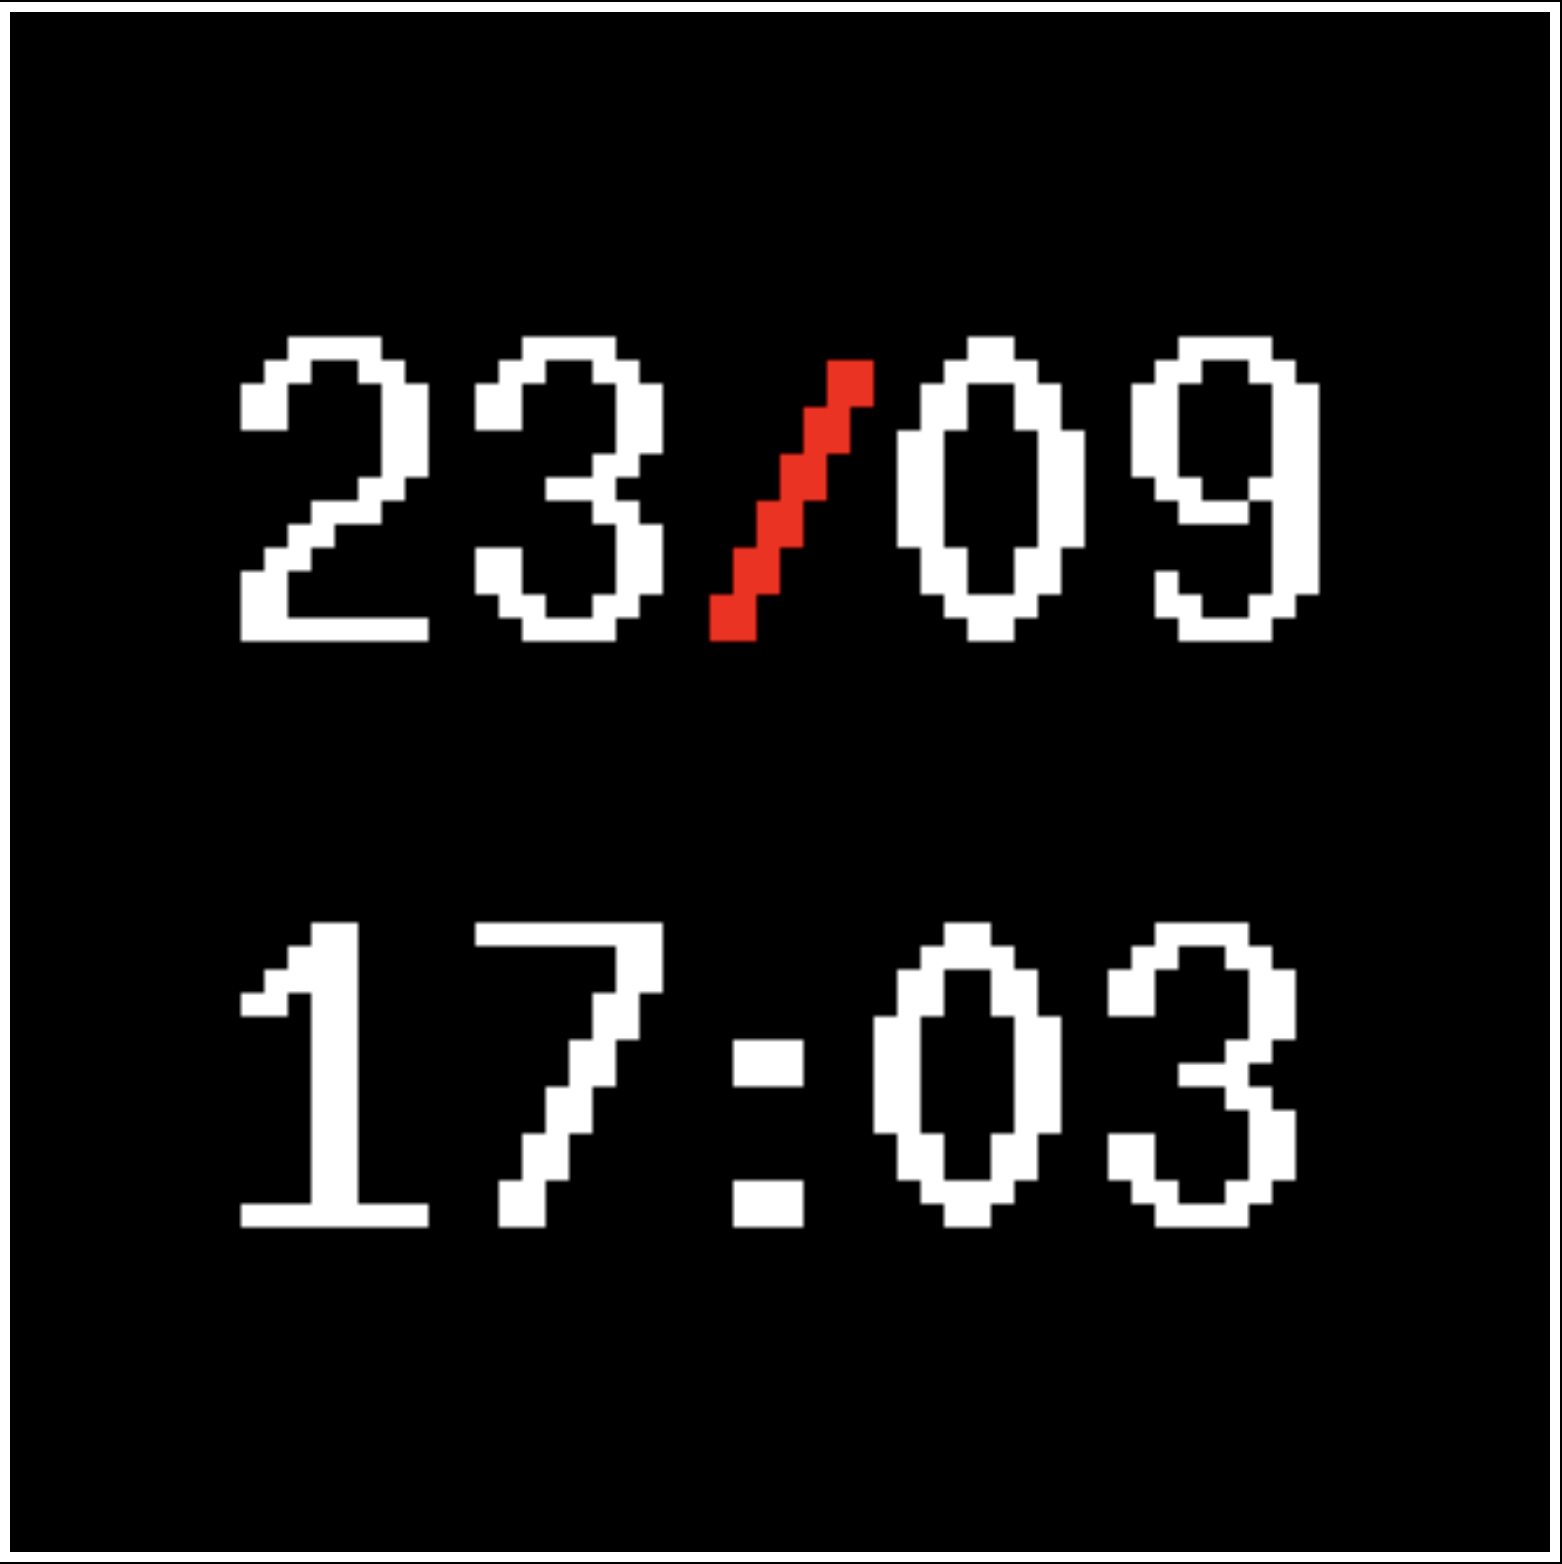
\includegraphics[width=\textwidth]{tesi/img/stylized_widgets/datetime.png}
        \caption*{\href{https://github.com/mosaico-widgets/date-and-time}{Date and Time} }
    \end{minipage}
    \begin{minipage}[b]{0.24\textwidth}
        \centering
        
\includegraphics[width=\textwidth]{tesi/img/stylized_widgets/dice.png}
        \caption*{\href{https://github.com/mosaico-widgets/d6}{Dice roll} }
    \end{minipage}
    \begin{minipage}[b]{0.24\textwidth}
        \centering
        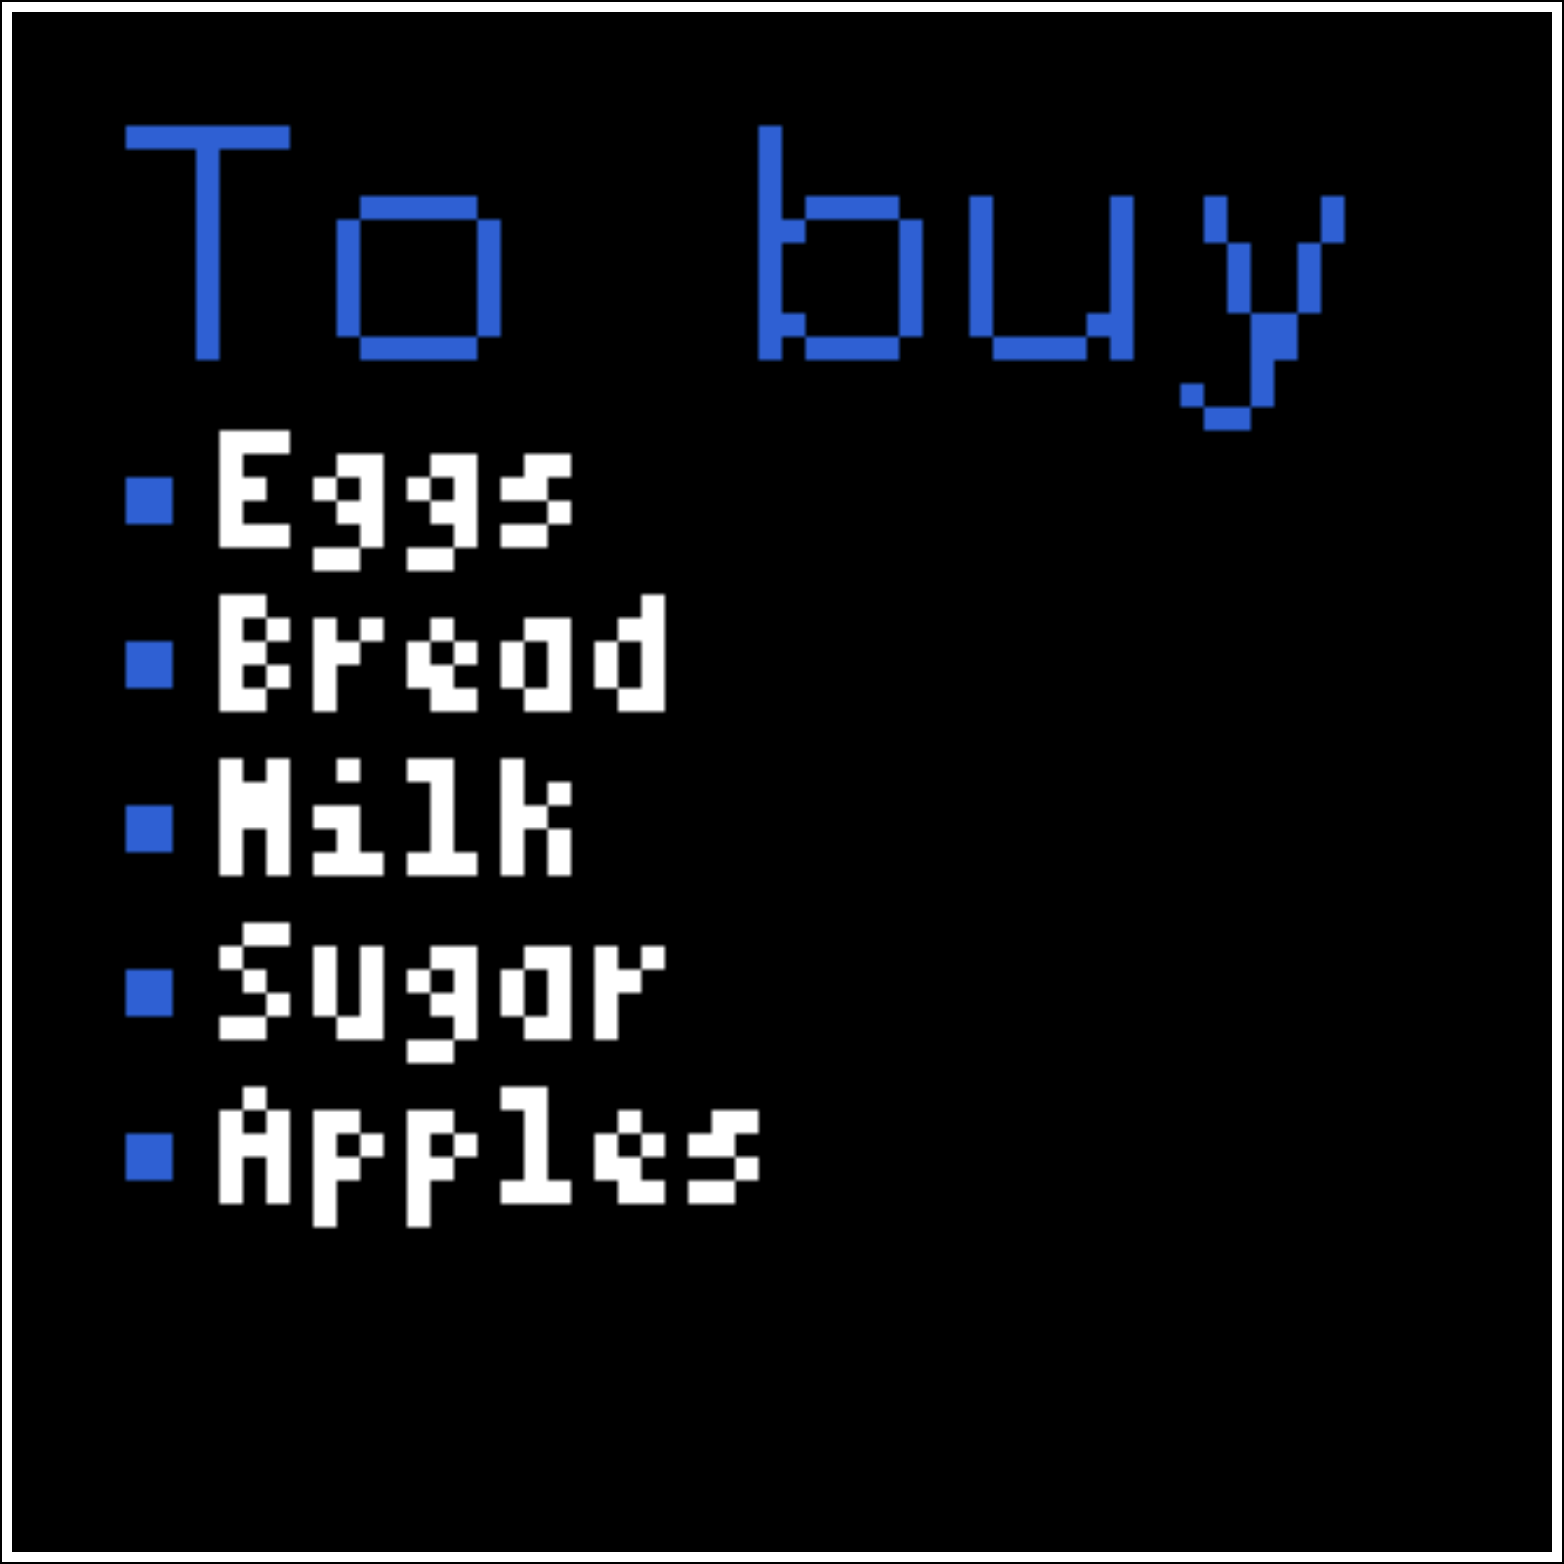
\includegraphics[width=\textwidth]{tesi/img/stylized_widgets/lists.png}
        \caption*{\href{https://github.com/mosaico-widgets/list}{List} }
    \end{minipage}
\end{figure}

The platform consists of multiple applications that work together seamlessly to deliver dynamic, customizable content to a Raspberry Pi-driven LED matrix.

\section{Motivation}
The growing demand for interconnected devices capable of communication in constrained environments has fueled the rapid expansion of the Internet of Things (IoT). As a tech enthusiast, I was naturally drawn to this world when I moved into my own home, where I sought to make every electronic device “smart” futhermore, I have always enjoyed having control centralized in a single place, like a dashboard—somewhere I can display dynamic information for everything I want to monitor.

Nevertheless, building a real-time content display system in an IoT environment presents several challenges, such as constrained bandwidth and low computational power. This thesis focuses on overcoming these obstacles by developing an IoT-based display system that leverages CoAP and BLE to efficiently deliver real-time dynamic content to an LED matrix driven by a Raspberry Pi.



\section{Open Source}
The Mosaico project has been developed and released under the AGPL-3.0 license, a copyleft open-source license designed to ensure that modifications and derivative works are freely available to the community. The full project code, including the various components of the platform, is publicly accessible for review, modification, and redistribution. The project's source code is organized and hosted on GitHub and can be found at the following \footnote{\url{https://github.com/orgs/mosaico-matrix}}. Additionally, a separate organization dedicated to the collection and publication of community-created widgets is available \footnote{\url{https://github.com/orgs/mosaico-widgets/}}.

Open-source software plays a pivotal role in advancing technological innovation and promoting collaborative development. By adopting an open-source model, Mosaico not only enables users to benefit from the transparency and adaptability of the software but also fosters an ecosystem where developers and hobbyists alike can contribute enhancements, fix bugs, and create new functionalities that serve the needs of the broader community. This collective effort accelerates the development process, often yielding more secure, stable, and feature-rich software than proprietary alternatives.

Furthermore, the Mosaico ecosystem is designed to embrace these open-source values not only in the core platform but also in the development and sharing of widgets. 

By leveraging the open-source model, Mosaico aspires to build a self-sustaining, innovative community that thrives on shared knowledge and collective growth.

\chapter{State of the art}
The concept of a remote-controlled LED matrix is not new, with numerous products available on platforms such as Amazon, and even more on Aliexpress. Typically, these products consist of a basic LED matrix combined with a mobile application, offering a limited range of functionalities. These usually include image display, clock features, and simple text scrolling, forming a standard set of operations that is largely identical across the various models on the market.

However, I quickly realized that none of these commercial solutions met my expectations. These devices are \textit{closed systems}, restricting customization options and preventing users from adapting the system to their specific needs or preferences. This restrictive nature severely limits the potential for innovation and creativity, which is essential for users seeking more than just basic functionality.

This lack of flexibility, combined with my growing passion for open-source software—where users and developers are key contributors—led me to create \textbf{Mosaico}. Unlike proprietary solutions, Mosaico is built around the principles of openness and customizability, offering users full control over the system. Inspired by well-known open-source projects such as Homebridge\footnote{Homebridge: \url{https://homebridge.io/}} and Flipper Zero\footnote{Flipper Zero: \url{https://flipperzero.one/}}, I envisioned an environment where both users and developers could collaboratively expand the system's capabilities.

Another key advantage of Mosaico is its affordability. The hardware components required to build the platform are both inexpensive and widely available, making the system accessible to a broad range of users. In contrast to the high costs often associated with commercial LED matrix products, Mosaico runs on simple, off-the-shelf components like the Raspberry Pi Zero W or similar single-board computers (SBCs) and a standard LED matrix. These components, readily available through various retailers, offer a cost-effective solution without sacrificing functionality.

Moreover, the open-source nature of the project ensures that software updates and improvements are continuously developed by the community, free of charge. Users are no longer dependent on a single vendor for updates or feature expansions, avoiding subscription fees or costly upgrades, as is often the case with commercial systems. This approach democratizes the technology, allowing hobbyists, developers, and individuals alike to experiment, create, and innovate without significant financial barriers.

In summary, Mosaico's reliance on inexpensive, easily sourced components not only makes it a highly cost-effective alternative to commercial LED matrix solutions, but it also reinforces the project's core mission: to empower users to fully customize, extend, and share their creations, all while keeping expenses to a minimum. This affordability, combined with the open-source ethos, positions Mosaico as a flexible, powerful, and budget-friendly option for anyone looking to explore the full potential of LED matrices.


\chapter{Objectives}

This project is aimed at building three major components, each with its own specific requirements
and constraints:

\section{Mobile app}

The end-user interface for discovering new widgets,
installing them, displaying them on the matrix device, controlling the
matrix, and checking its status.

\begin{itemize}
    \item \textbf{Ease of use}: The app must be intuitive, visually appealing,
        and easy to navigate.

    \item \textbf{Performance}: It should be fast, responsive, and reactive to
        user inputs, providing a seamless experience.

    \item \textbf{Automatic Device Discovery}: The app should automatically discover
        and pair with the matrix device to simplify the user experience.

    \item \textbf{Caching Mechanisms}: To minimize resource consumption on the
        constrained matrix device, the app must implement caching strategies
        that reduce unnecessary data requests and processing overhead.
\end{itemize}





\section{Raspberry Pi Software}

This is the core software running on the
Raspberry Pi, responsible for communicating with the mobile app and
controlling the LED matrix through hardware wiring. \label{software-objectives}
  
\begin{itemize}
    \item \textbf{Efficiency}: The software must be optimized for power and memory
        usage, given the limited resources of the Raspberry Pi.

    \item \textbf{Modularity and Customizability}: The system should be modular,
        allowing developers to easily create and add new widgets dynamically, without the need of a re-compilation.

    \item \textbf{Documentation}: Clear and detailed documentation is essential
        to guide developers who wish to create or modify widgets, ensuring the
        platform’s extendibility.
\end{itemize}



\section{Web Platform}
This encompasses the REST API for the widget store,
the project website, documentation, and the developer dashboard for
uploading and managing widgets.

\begin{itemize}
    \item \textbf{Deployment}: The web platform should be easily deployable on
        standard cloud or on-premise environments.

    \item \textbf{Design}: The user interface should be intuitive and visually
        appealing to enhance user engagement and usability.
\end{itemize}


\section{Additional Features}
Beyond the core components, I thought of additional features to further enhance
the project:
\begin{itemize}
\item \textbf{Simulator}: Allow users to have a playground to try out things before buying the actual hardware matrix (or to speed up the development of widgets)

\item \textbf{IDE}: A dummy Desktop software to rapidly get into widget development, providing a widget template and an easy connection to the matrix to preview and debug widgets
  
	\item \textbf{Cross-Platform Support}: Ensure that the mobile app functions seamlessly
		across multiple platforms (iOS, Android and Desktop)

	\item \textbf{Extensibility}: The project should be designed in a way that makes
		it easy to integrate additional features or technologies (e.g., adding
		support for more IoT protocols or other smart devices).

	\item \textbf{Community Engagement}: Actively engage with the open-source community
		through forums, contribution guidelines, and issue tracking to foster collaboration
		and improve the project over time.
\end{itemize}

\chapter{Project architecture}
\begin{center}
  \makebox[\textwidth]{
  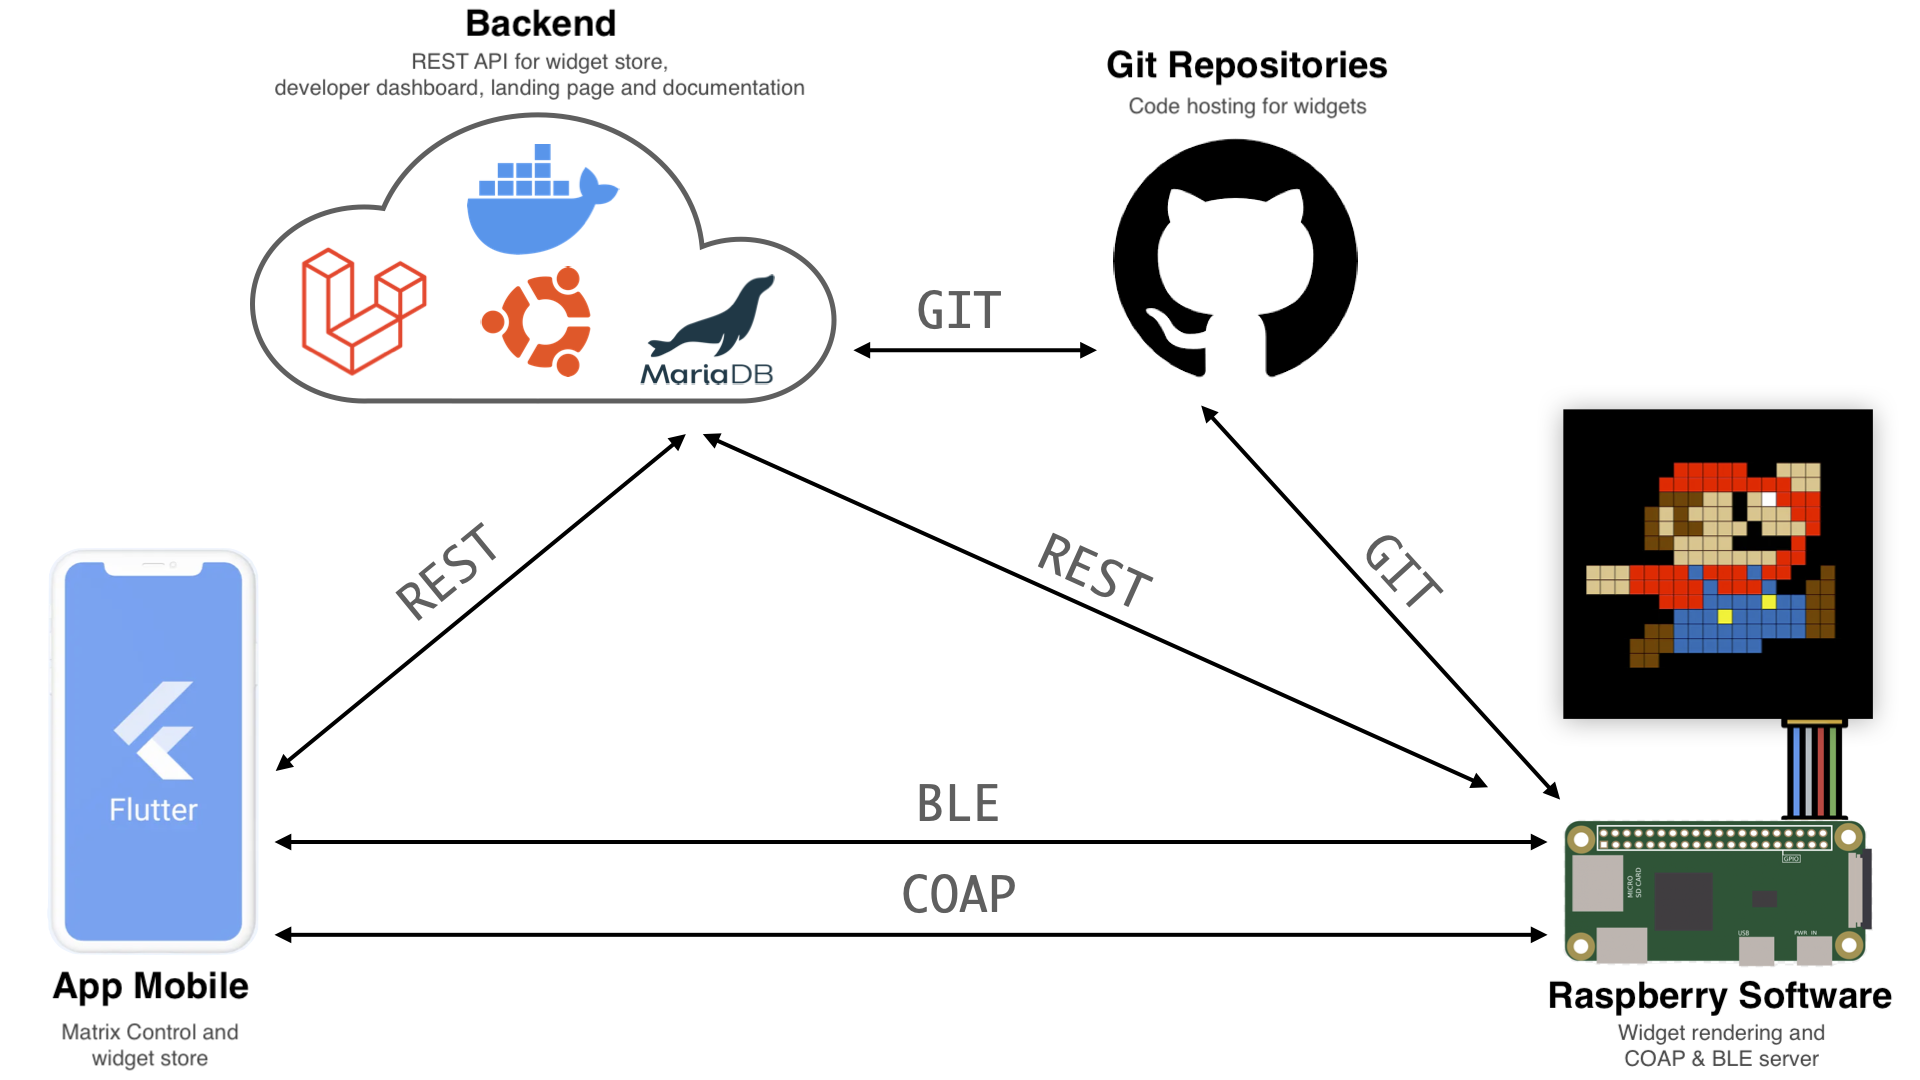
\includegraphics[width=0.8\paperwidth]{tesi/img/software-arch.png}
  }
\end{center}

\section{Networking}
When developing an IoT project, selecting an appropriate networking stack is a crucial design consideration. In the case of Mosaico, this choice is particularly significant due to the system's diverse components and their interactions. It is essential to evaluate communication protocols carefully to achieve an optimal balance among performance requirements such as speed, resource efficiency, and functionality while considering the limitations imposed by the hardware and specific use cases. Each layer of the networking stack fulfills a distinct role, and a well-structured combination of protocols is necessary to ensure that the system operates efficiently and remains scalable over time.

\subsection{Constrained Application Protocol (COAP)}

The primary communication protocol used in Mosaico between the mobile application and the Raspberry Pi is the Constrained Application Protocol \cite{rfc7252} (COAP). COAP is an Internet Engineering Task Force (IETF) standard designed explicitly for constrained devices in IoT environments, and it proved to be a more suitable alternative to previously considered options like raw TCP sockets and REST-based servers.

Initially, the project employed a basic TCP socket for communication, providing low-level control over data transfer between the mobile app and the Raspberry Pi. While TCP sockets offer the advantage of simplicity and direct control, they lack the higher-level abstractions and features that are essential for a scalable and maintainable architecture. Communication over raw sockets quickly became cumbersome and error-prone due to the absence of structured methods for defining request/response patterns, error handling, and state management.

In an attempt to overcome these limitations, the next iteration of the project moved towards implementing a traditional REST server on the Raspberry Pi. REST, based on HTTP, is a well-established protocol that provides an organized method for communication through well-defined endpoints using methods like GET, POST, PUT, and DELETE. It allowed for more structured interaction between the mobile app and the Raspberry Pi, introducing features like query parameters, headers, and status codes. However, while REST is robust, it is also relatively resource-heavy. Running a fully-fledged REST server on the Raspberry Pi, a resource-constrained device, proved to be overkill for the application’s needs. The overhead of managing HTTP headers, complex request/response formats, and other RESTful conventions unnecessarily taxed the Raspberry Pi’s limited processing power and memory.

The inefficiency of using REST on constrained hardware prompted a deeper exploration of alternatives, leading to the introduction of COAP, a protocol tailored for constrained environments. My supervisor suggested COAP as a middle ground between the simplicity of raw TCP and the complexity of REST, and it has since become the core protocol for communication in Mosaico.

COAP is a specialized web transfer protocol designed for use in IoT environments, offering a much lighter alternative to REST while retaining many of its familiar semantics. COAP follows the same request-response model as REST, supporting methods like GET, POST, PUT, and DELETE, and allows for interaction with endpoints using URIs. However, COAP significantly reduces the protocol overhead by employing a binary message format instead of the text-based HTTP. Additionally, COAP runs over UDP instead of TCP, making it more lightweight and responsive, especially in scenarios where reliable packet delivery is not critical for every message.

In practical terms, COAP provided Mosaico with a streamlined and efficient communication stack that did not impose the same processing and memory overheads as HTTP-based REST. It offered the right balance between simplicity and structure, making it a perfect fit for the constrained environment of the Raspberry Pi. Moreover, COAP allows arbitrary payloads to be transmitted, enabling flexible communication patterns between the mobile app and the Raspberry Pi without introducing unnecessary complexity.


\subsection{Bluetooth Low Energy (BLE)}

While COAP forms the backbone of the communication between the mobile app and the Raspberry Pi, it relies on an IP-based protocol, which necessitates that the Raspberry Pi be connected to a network and that its IP address is known to the app. However, in practical scenarios, especially during initial setup, the Raspberry Pi may not yet be connected to the internet or assigned an IP address. This posed a critical challenge in ensuring a seamless and intuitive setup experience.

At first, I considered two potential solutions: 

\begin{enumerate}
    \item Configure the Raspberry Pi as a WiFi access point, allowing the mobile app to communicate directly with it via a local connection.
    \item Utilize a different communication method that does not rely on a router or existing network connection.
\end{enumerate}
The first approach, while feasible, was discarded because setting up the Raspberry Pi as a WiFi access point seemed somewhat convoluted and less elegant. Instead, I chose to implement a Bluetooth Low Energy (BLE) solution, which offered a more straightforward and reliable way to handle the initial setup without requiring any pre-existing network configuration.

In this BLE-based approach, the Raspberry Pi operates a GATT (Generic Attribute Profile) server alongside the COAP server. The BLE server is primarily responsible for three main tasks:

\begin{enumerate}
    \item \textbf{Discovery}:The BLE server advertises a service that the mobile app can detect during a BLE scan. This allows the app to discover the nearby Raspberry Pi without needing its IP address or requiring internet connectivity.
    \item \textbf{Wi-Fi Configuration}: Once connected via BLE, the mobile app can send Wi-Fi credentials (SSID and password) to the Raspberry Pi, allowing it to join a network. This eliminates the need for manual configuration, simplifying the setup process significantly.
    \item \textbf{IP Address Retrieval}: After the Raspberry Pi connects to the network, the mobile app can request the local IP address through BLE. The Pi responds with its IP, enabling the app to switch over to COAP for further communication.
\end{enumerate}
This BLE implementation was a game-changer in the Mosaico setup process, allowing users to quickly and easily connect the Raspberry Pi to their local network without needing to interface with routers or manually configure network settings. BLE's low power and short-range capabilities made it ideal for this purpose, offering a seamless handoff to COAP once the network connection was established.

This approach demonstrates how BLE can complement IP-based protocols like COAP in IoT environments by handling the initial device discovery and configuration stages, creating a more user-friendly and efficient setup experience.

\subsection{GIT Integration for Widget Management}

One of the core principles behind Mosaico is maintaining openness and accessibility within the ecosystem. To ensure that all community-contributed widgets remain open source—and to also minimize storage demands on the Mosaico server—the download and distribution of widgets from the app store to the Raspberry Pi is handled via public GIT repositories.

When developers create a widget, they can link their repository directly to the widget's entry on the Mosaico developer dashboard. This means that users downloading the widget from the app store are pulling the most up-to-date version directly from the developer’s public GIT repository.

This method not only promotes transparency by allowing anyone to browse the widget’s source code but also simplifies maintenance for developers. When they push new updates to their repository, the changes are automatically reflected in the app store, allowing users to seamlessly update their installed widgets.

By leveraging GIT, Mosaico fosters a collaborative, open-source environment where the community can share, improve, and build on each other’s work with minimal friction.

\subsection{REST}

The REST protocol is another key component utilized in Mosaico, primarily for communication between the mobile app and the Mosaico store API. As a widely-adopted protocol, REST is an ideal choice for exchanging structured data in a lightweight format like JSON. This ensures compatibility and ease of integration between different components of the Mosaico ecosystem.

On the mobile app side, REST facilitates smooth interactions with the app store, allowing users to browse, search for, and manage widgets. REST also serves the Raspberry Pi software when a user installs a new widget. When an installation request is made, the Pi retrieves essential information—such as the GIT repository URL where the widget’s source code is hosted and other relevant metadata—via the REST API. This data is then stored in a local indexed database for future use, ensuring that Mosaico remains responsive even when offline.

The decision to use REST here is guided by the need for a reliable, feature-rich, yet easy-to-use communication protocol. This setup allows Mosaico to seamlessly integrate the app store with the Raspberry Pi, offering a smooth experience for both developers and end users.
\section{Widgets}
Widgets are the central primitive of the Mosaico ecosystem. They can be thought of as small applications that users can search for, install, and run locally on their matrix through the app store. The Mosaico platform allows anyone to contribute by developing widgets via the developer portal, requiring only a basic knowledge of Python.

\subsection{Widget Types}
Mosaico widgets are categorized into three distinct types:
\label{widget-types}
\begin{figure}[h]
    \centering
    \begin{minipage}[b]{0.32\textwidth}
        \centering
        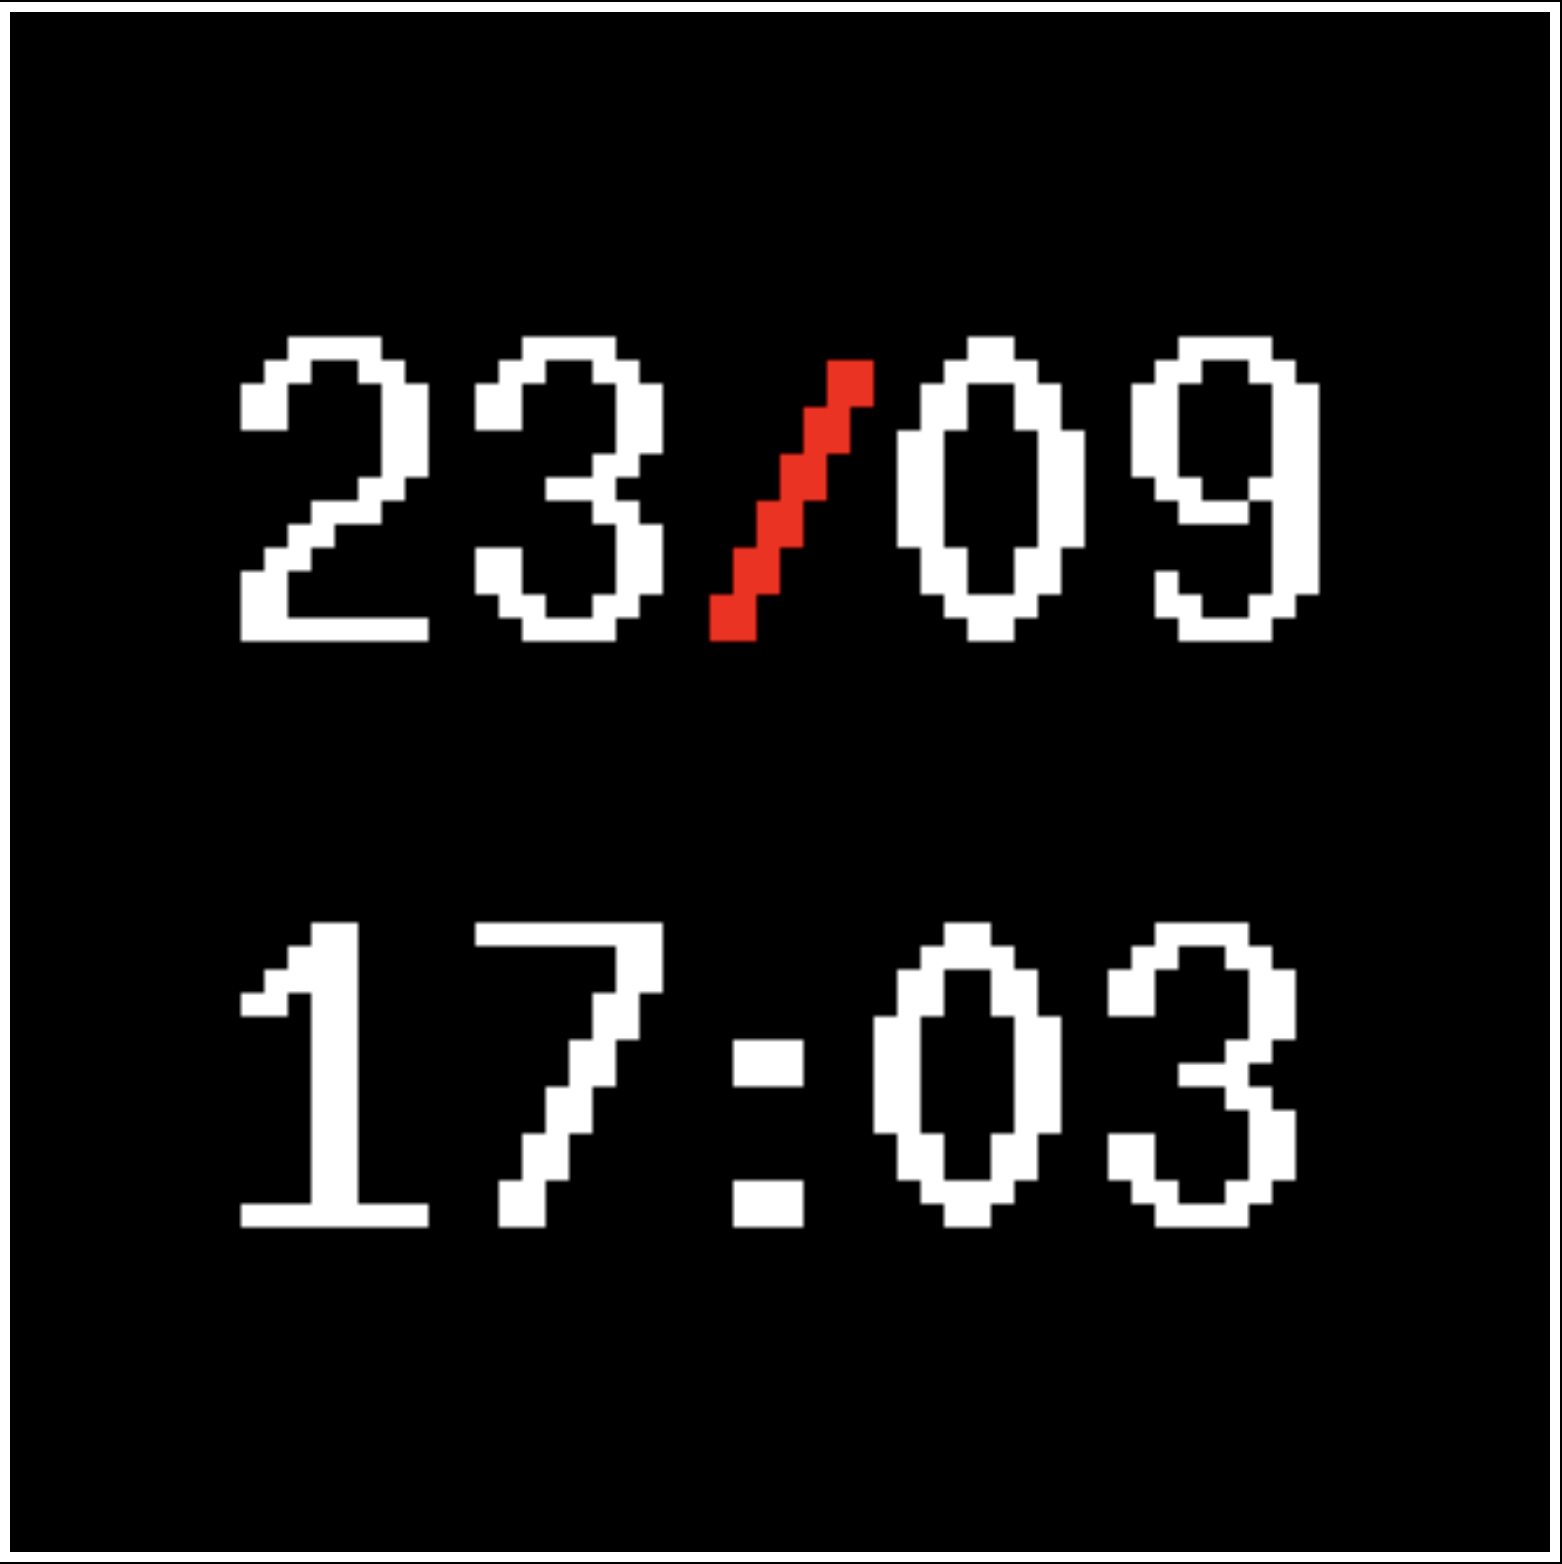
\includegraphics[width=\textwidth]{tesi/img/stylized_widgets/datetime.png}
        \caption*{\textbf{Static Widgets}\newline These can be displayed on the matrix immediately upon installation.}
    \end{minipage}
    \begin{minipage}[b]{0.32\textwidth}
        \centering
        
\includegraphics[width=\textwidth]{tesi/img/stylized_widgets/image.png}
        \caption*{\textbf{Configurable Widgets}\newline These require additional configuration before they can be displayed.} 
    \end{minipage}
    \begin{minipage}[b]{0.32\textwidth}
        \centering
        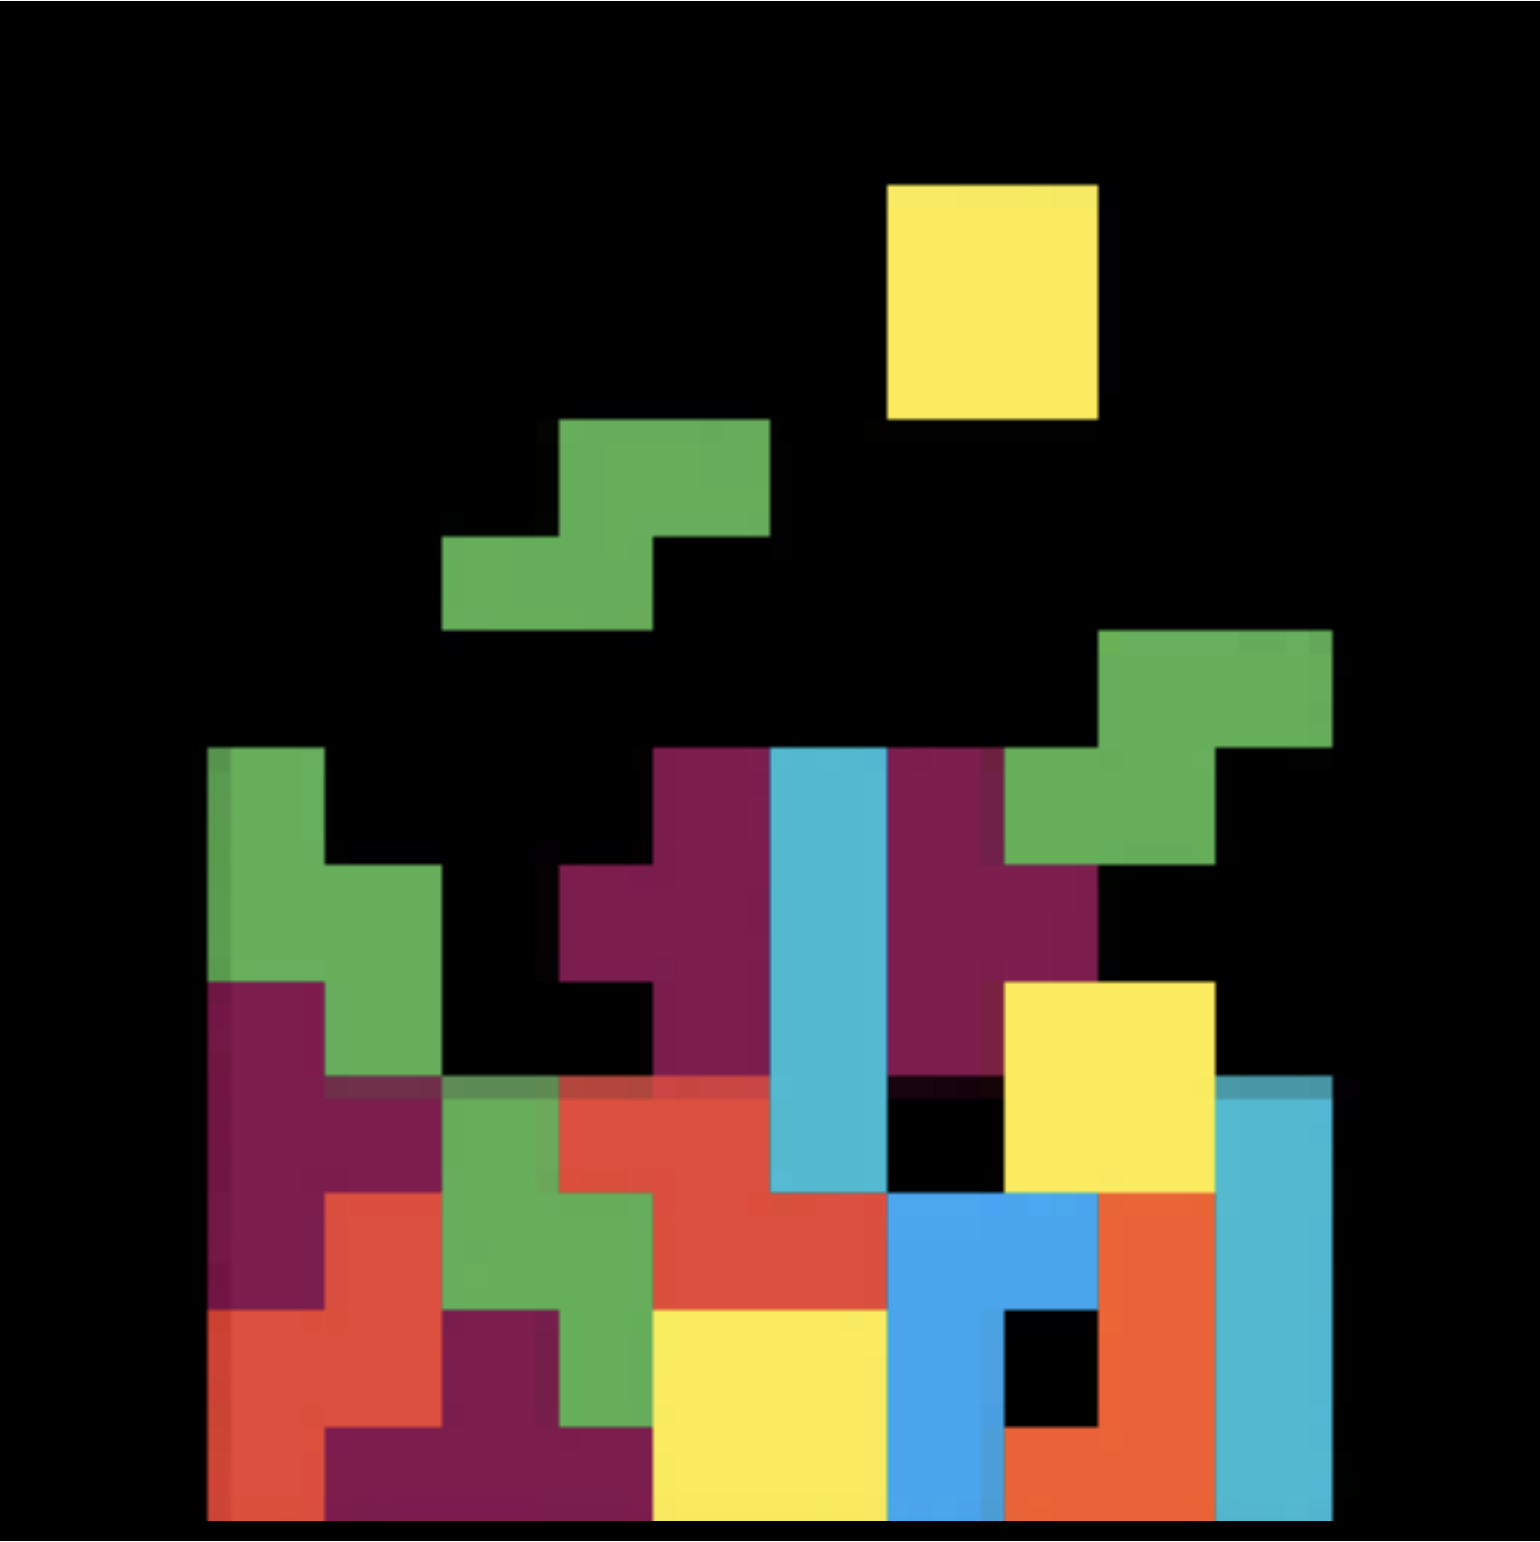
\includegraphics[width=\textwidth]{tesi/img/stylized_widgets/tetris.png}
        \caption*{\textbf{Dynamic Widgets}\newline These require real-time user interaction while they are being displayed.}
    \end{minipage}
\end{figure}

\subsection{Anatomy of a Widget}
We stated what the widgets are and how they play a central role inside the Mosaico ecosystem but how are they actually made?
At their core, Mosaico widgets are projects comprised of three primary components:

\begin{enumerate}
    \item \textbf{Widget Script}: This is the core of the widget, written in Python, and is responsible for rendering visuals on the matrix.

\begin{minted}{python}
# Simple example of a widget that displays "Hello World"
# It retrieves its configuration from the config form
from mosaico import widget, config

# Create text
text = widget.createText()
text.setText(config["text"])
text.setHexColor(config["color"])
text.setFont(config["font"])
text.moveTo(2,30)

# No need to update each frame
def loop():
    pass
\end{minted}

    \item \textbf{Configuration Form}: A JSON file that defines a form to be presented in the client app, collecting input from the user if the widget requires configuration.

\begin{minted}{json}
{
  "form": {
    "title": "Text",
    "description": "Write custom text on the matrix.",
    "fields": [
      {
        "text": {
          "type": "string",
          "label": "Text",
          "required": true,
          "placeholder": "Enter the text you want to display"
        },
        "color": {
          "type": "color",
          "label": "Color",
          "required": true,
          "placeholder": "Choose the color for the text"
        },
        "font": {
          "type": "font",
          "label": "Font",
          "required": true,
          "placeholder": "Select a font"
        }
      }
    ]
  }
}
\end{minted}
\newpage
    \item \textbf{Metadata}: This is a manifest file written in JSON, containing essential information for both the rendering engine (e.g., frame rate, whether the widget is configurable) and the app store platform (e.g., widget name, description, version).

\begin{minted}{json}
{
  "name": "Text",
  "description": "Displays custom text on the matrix.",
  "widget_version": "1.0",
  "software_version": "1.0",
  "author": "murkrow",
  "fps": 20,
  "configurable": true
}
\end{minted}
\end{enumerate}





\chapter{The Hardware}
The first challenge I faced while designing the project was finding the best yet cheapest hardware to power the system efficiently, ensuring it could handle the required tasks without exceeding budget constraints, while also providing flexibility and scalability for future upgrades.

\begin{figure}[h]
    \centering
    \begin{minipage}[b]{0.32\textwidth}
        \centering
        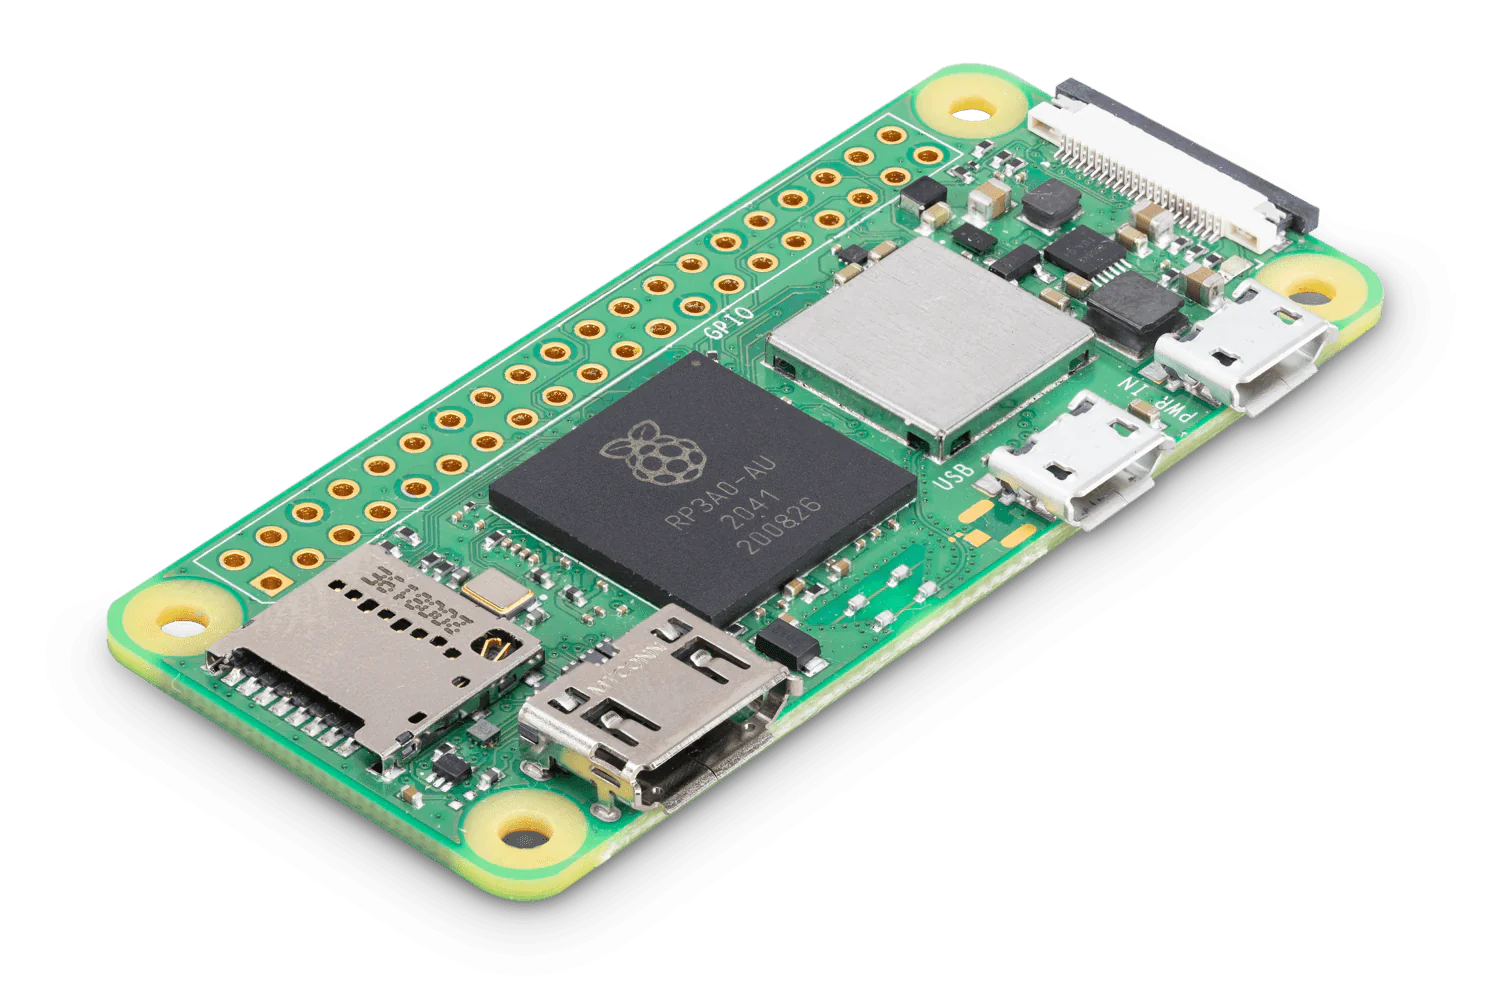
\includegraphics[width=\textwidth]{tesi/img/hardware_components/rpi.png}
        \caption*{Raspberry Pi Zero W}
    \end{minipage}
    \begin{minipage}[b]{0.32\textwidth}
        \centering
        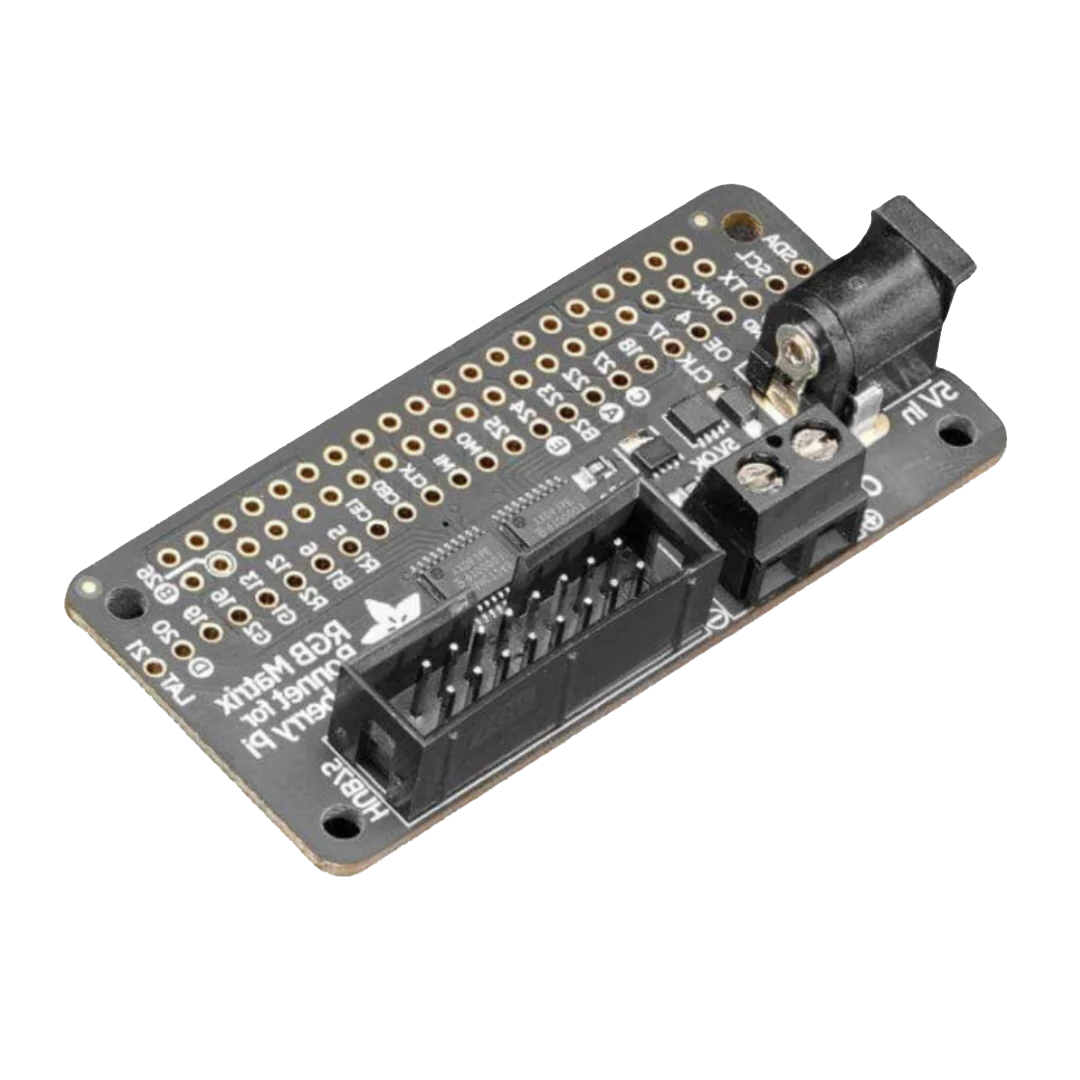
\includegraphics[width=\textwidth]{tesi/img/hardware_components/bonnet.png}
        \caption*{Adafruit RGB Matrix Bonnet}
    \end{minipage}
    \begin{minipage}[b]{0.32\textwidth}
        \centering
        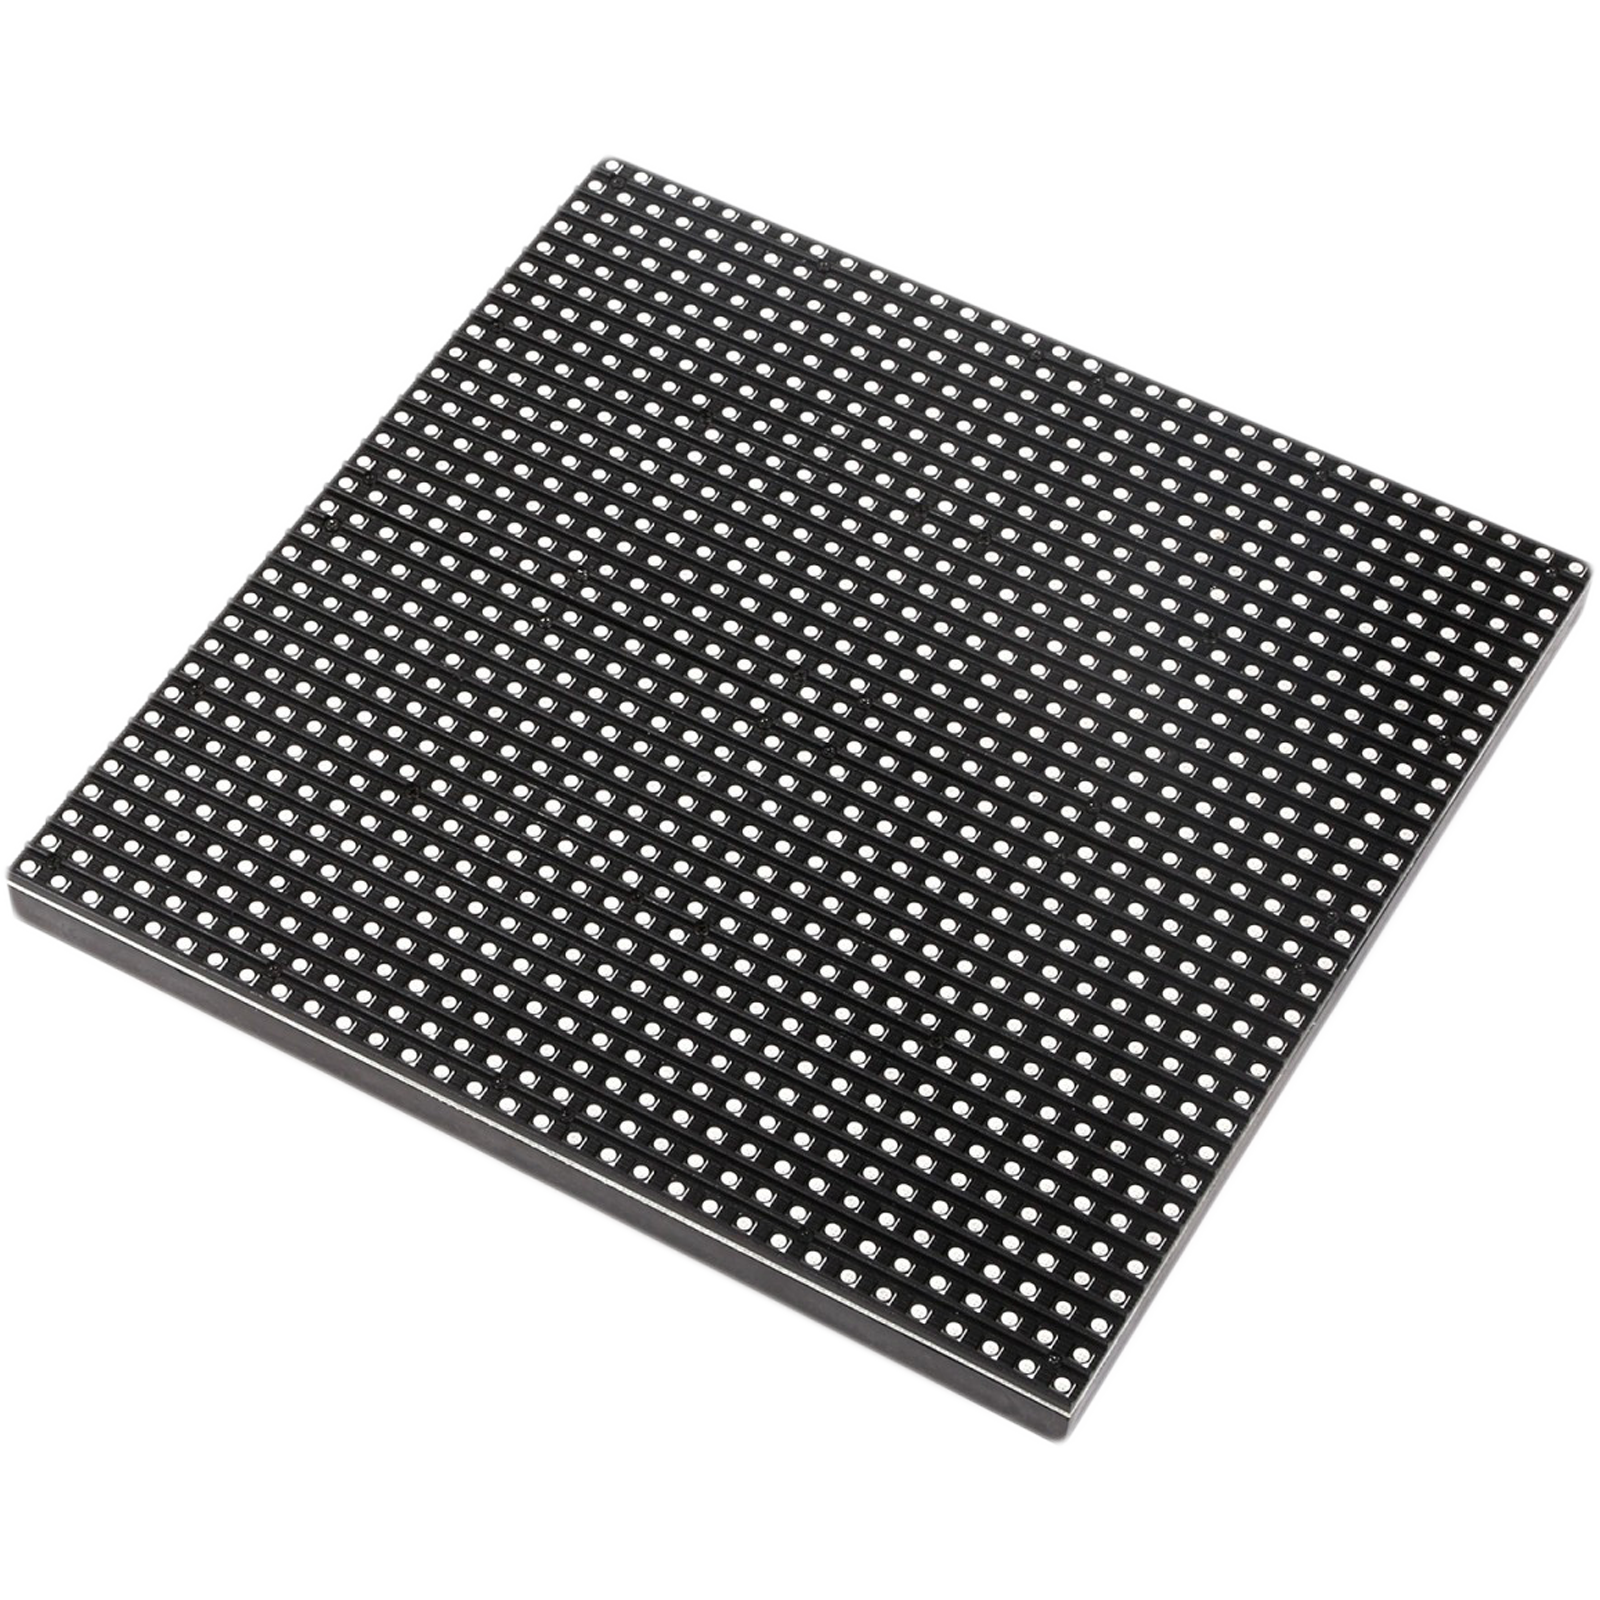
\includegraphics[width=\textwidth]{tesi/img/hardware_components/matrix.png}
        \caption*{Standard 64x64 LED Matrix}
    \end{minipage}
\end{figure}


\section{The SBC}

The most critical decision was selecting the processing unit,
and I realized that I needed a single-board computer (SBC) with the following
characteristics:

\begin{itemize}
	\item Sufficient computational power for handling both graphical rendering and networking operations

	\item Broad connectivity options, such as WiFi, Bluetooth, and GPIO pins for
		external peripherals

	\item Cost-effective, as affordability was a primary concern

	\item Highly customizable, to allow flexible development and integration with
		other components
\end{itemize}

Initially, I considered two options: the \textbf{Raspberry Pi} and the \textbf{ESP32}, both
equipped with built-in Bluetooth and WiFi. The ESP32 is a fantastic microcontroller, known for its low power consumption and versatility in IoT applications. It's gaining immense popularity due to its ultra-low cost—priced as low as 5 euros—yet powerful enough to build impressive and innovative projects.
However,
after evaluating my project’s requirements, I opted for the Raspberry Pi Zero W due
to its Linux support, which I believed would provide better flexibility and
facilitate more advanced functionalities, such as running a full operating system,
handling networking tasks, and interacting with various software libraries.

I chose the Raspberry Pi Zero W for several reasons:
\begin{itemize}
	\item \textbf{Operating System Support:} With a lightweight, CLI only Linux-based OS like \href{https://dietpi.com/}{DietPi}, I could leverage a vast ecosystem of software tools and libraries,
		enabling more complex operations that would be harder to achieve on a
		microcontroller like the ESP32.

	\item \textbf{Connectivity:} The Raspberry Pi Zero W comes with built-in WiFi
		and Bluetooth, making it ideal for connecting to the internet and integrating
		with other wireless devices.

	\item \textbf{Size and Power Consumption:} Despite being a fully capable
		computer, the Raspberry Pi Zero W is compact and consumes minimal power,
		which was important for keeping the hardware cost-effective and portable.

	\item \textbf{GPIO Pins:} The GPIO pins offer a wide range of possibilities
		for connecting sensors, LEDs, and other hardware components, making it easy to
		extend the platform with additional functionality.
\end{itemize}
\section{The Matrix}
When it came to selecting the LED matrix, I was faced with a wide array of options, each offering different resolutions, sizes, brands, and even color configurations. The first decision I had to make was regarding the resolution, which would directly impact the amount of information the display could render. The two primary options I considered were a rectangular 64x32 matrix or a square 64x64 matrix. After careful consideration, I ultimately chose the 64x64 matrix. This resolution struck the perfect balance for my needs: it wasn't too large, which kept the overall system compact and cost-effective, yet it provided enough screen real estate to display a substantial amount of information, ensuring that the display would be both functional and visually appealing.
\section{The Matrix Bonnet}
Although it would have been possible to manually wire the Raspberry Pi directly to the LED matrix, I decided to invest in the Matrix Bonnet for several reasons. For just a few euros, the bonnet offered a much safer, more reliable, and easier solution compared to manual wiring. It not only simplifies the connection process but also reduces the risk of damaging the components due to incorrect wiring. The Matrix Bonnet is specifically designed for use with Raspberry Pi boards, allowing for seamless integration and a cleaner, more stable setup. It handles all the necessary data and power connections without the hassle of complex wiring, which saved me significant time and effort during development. The bonnet is just one of the many incredible products developed by Adafruit Industries, which are designed to make open-source DIY projects like this not only accessible but also well-documented and enjoyable\footnote{\url{https://www.adafruit.com}}.

\section{Future Upgrades}
While the current setup meets the initial goals of the project, I have plans for several future upgrades to enhance both functionality and user experience. I am considering integrating new sensor types, such as environmental sensors or cameras, to add real-time data collection capabilities. 

\chapter{The Software}
One of the main challenges in developing the software was selecting the right programming language. As mentioned previously$^{\ref{software-objectives}}$, I needed the software to be both high-performing and flexible. A compiled language was essential, as a scripting language wouldn’t be able to handle the rendering of complex widgets, especially when trying to push the limited power of the Raspberry Pi to its limits. This led to the immediate exclusion of languages like Python and JavaScript. Although C and C++ were obvious choices due to their efficiency, I initially sought something more modern and sophisticated. However, after some experimentation, I found that the .NET runtime wasn’t suitable for the Pi, and alternatives like Java and Rust didn’t provide the same performance gains I achieved with C++ that in the end emerged as the best option.

\section{C++ Module}
I began by creating a minimal prototype capable of turning individual pixels on and off on the matrix. Fortunately, there was an excellent project on GitHub by Hzeller \footnote{\url{https://github.com/hzeller/rpi-rgb-led-matrix}} that offered a solid C++ implementation, covering the fundamental functionality I needed to get started, including: \begin{itemize} \item Direct manipulation of individual pixel colors \item Filling the entire matrix with color \item Creating an in-memory canvas to draw on while displaying something else on the matrix, allowing for smooth transitions when swapping \item Loading .bdf fonts and converting text to pixels \end{itemize}

Given the goal of providing modularity, it made sense to define a class that each Widget could inherit from, allowing them to implement their own methods. 
Each widget is designed to encapsulate its internal workings, exposing only a single method: \textit{renderNextFrame}. Similar to a sprite in a game engine, the widget’s responsibility is simply to determine where to paint pixels in the next frame—no more, no less. Here’s an example of a widget that draws a simple rectangle:

\begin{minted}{c++}
class RectangleWidget : public Widget
{
    int width, height, x, y;
    Color color;
    RectangleWidget(int width, int height, int x, int y, Color color)
    {
        this.width = width;
        this.height = height;
        this.x = x;
        this.y = y;
        this.color = color;
    }

    void renderNextFrame(Canvas *canvas)
    {
        for (int i = 0; i < width; i++) {
            for (int j = 0; j < height; j++) {
                canvas->SetPixel(x+i, y+j, color.r, color.g, color.b);
            }
        }
    }
}
\end{minted}
\newpage
At this point my application is very simple but working and it looks something like this:

\begin{minted}{c++}
int main(int argc, char *argv[]) {

    Logger::logInfo("Mosaico is starting");

    // Init matrix
    RGBMatrix::Options matrix_options;
    matrix_options.rows = 64;
    matrix_options.cols = 64;
    // Other config stuff

    // Create matrix object
    RGBMatrix *matrix = RGBMatrix::CreateFromOptions(matrix_options);

    // Create a widget
    Widget runningWidget = new RectangleWidget(w,h,x,y,color);

    // Main loop
    while (true) {
        matrix->clear();
        runningWidget->renderNextFrame(matrix);
        // delay here to ensure 30Hz refresh rate
    }
}
\end{minted}
\subsection{The Canvas} As you may have noticed, the \textit{renderNextFrame} method accepts a \textit{Canvas} object as a parameter instead of directly manipulating the matrix. This approach aligns with one of the SOLID principles: \textbf{dependency inversion} \cite{dep_inv_principle}. The widgets do not need to know the specifics of the matrix; they interact with it as if it were a simple canvas to paint on. This abstraction not only simplifies the widget code but also allowed for greater flexibility as the project evolved.

\subsection{Drawables}
\label{widget_canvas_abstraction}
As I continued developing widgets, I found myself repeatedly writing similar code, particularly for drawing shapes and text. This repetition led to the creation of the \textbf{Drawable} concept—a base class that allowed me to store common shapes and figures as objects. This abstraction made it easier to create and manipulate these elements consistently across different widgets.

The \textit{Drawable} class encapsulates shared functionality such as position, color, and animation, providing a unified interface for handling visual elements. Here's a simplified structure of the \textit{Drawable} class hierarchy:

\begin{center}
  \makebox[\textwidth]{
  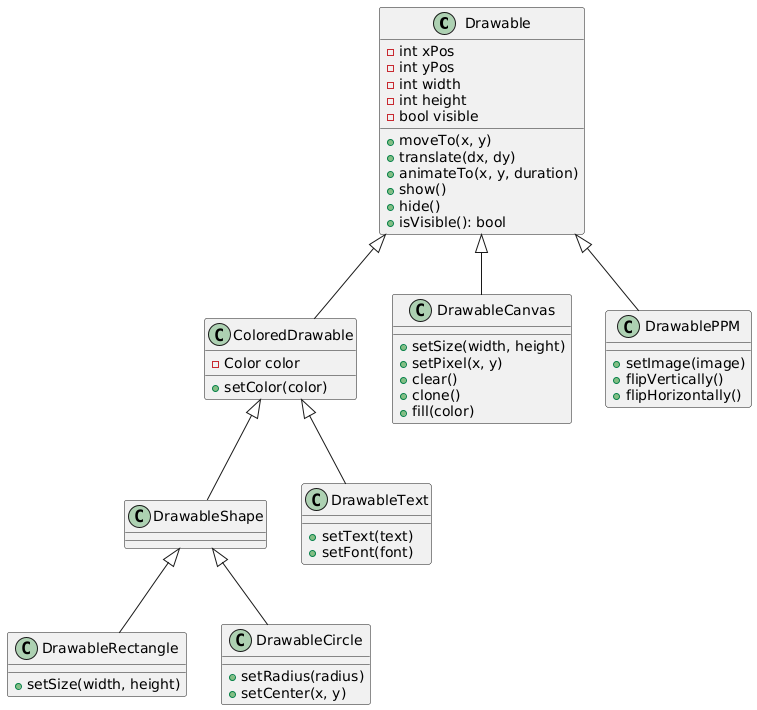
\includegraphics[width=0.8\paperwidth]{tesi/img/drawables.png}}
\end{center}

\newpage

At this point I had to edit the \textit{Widget} class in order to correctly register and render drawables.


\begin{minted}{c++}

class Widget {
private:
     // Drawables to be rendered
    std::vector<Drawable*> registeredDrawables;    
public:
    /// Add a new drawable to the widget drawable list
    void registerDrawable(Drawable* drawable);
    /// Remove a drawable from the widget drawable list
    void unregisterDrawable(Drawable* drawable);
    /// Clear all drawables
    void clearDrawables();

    void renderNextFrame(Canvas* canvas) {
        // Call the inheriting widgets to do their job
        render(canvas);
        // Drawables should be now updated, draw them
        for (Drawable* drawable : registeredDrawables) {
            drawable->draw(canvas);
        }
    }
protected:
    Widget();
    /// Pure virtual method to be overridden inheriting widgets for rendering
    virtual void render(Canvas* canvas) = 0;
};
\end{minted}

This basic setup was enough to get things up and running, enabling me to create more complex widgets.

\subsection{Loading Widgets at Runtime} At this stage, I had a straightforward method for creating new widgets and drawing shapes efficiently. If someone wanted to contribute to the project and add a new widget, they would clone the project, create a new C++ class that inherits from \textit{Widget}, write the necessary code, compile the app again, and submit a pull request.

While this approach would work, it lacked flexibility. Every time a developer added a new widget, users would need to update their software to access it. This wasn't ideal for a modular and dynamic system.

In a meeting with my supervisor, we explored the idea of treating widgets like "plug-ins" or encoded strings that the C++ program could decode in real time to display dynamic content. Although this concept was easier said than done, the potential excited me, and I immediately began experimenting with different approaches to find the best solution.

\subsubsection{Custom Encoding} My first thought was to create a custom encoding format for widgets, something akin to JSON or YAML but optimized for my needs. I imagined a frame-based system where I could specify what to render at each frame, perhaps even introducing a simple mock language to handle loops and conditionals. However, this approach proved too limiting and complex, especially for achieving the flexibility I desired. It was soon discarded.

\subsubsection{Lua vs. ChaiScript} I quickly realized that the only way to provide developers with the maximum flexibility for widget creation was to embed a Turing-complete scripting language. Drawing from my limited knowledge of game development, I knew that popular games often use Lua for custom levels and dynamic content creation \footnote{\url{https://create.roblox.com/docs/scripting}}.

Lua, being lightweight and having a C-based interpreter, seemed like a good candidate. I embedded Lua into my application, allowing it to interface with my C++ code. Initially, this appeared to be the solution, but several issues arose:

    \begin{itemize}
        \item Integration complexity: Mapping complex C++ types such as drawables, the canvas, and various helper functions to Lua proved cumbersome and overcomplicated.
        \item Syntax dissatisfaction: I found Lua's syntax unintuitive and less modern than I wanted for widget development. I aimed for a scripting language that would feel clean, readable, and enjoyable to write.
    \end{itemize}

After further research, I discovered ChaiScript \footnote{\url{https://chaiscript.com/}}, a lightweight, JavaScript-like embedded scripting language designed specifically for C++. Its integration was much simpler than Lua, with easier mapping of types and classes. I liked how the implementation was progressing, and I finally got a working solution. Below is a demo of the first widget written in ChaiScript, where I comment out parts of the code in real-time, and they are rendered immediately on the matrix!

\begin{figure}[h] \centering \begin{minipage}[b]{0.49\textwidth} \centering 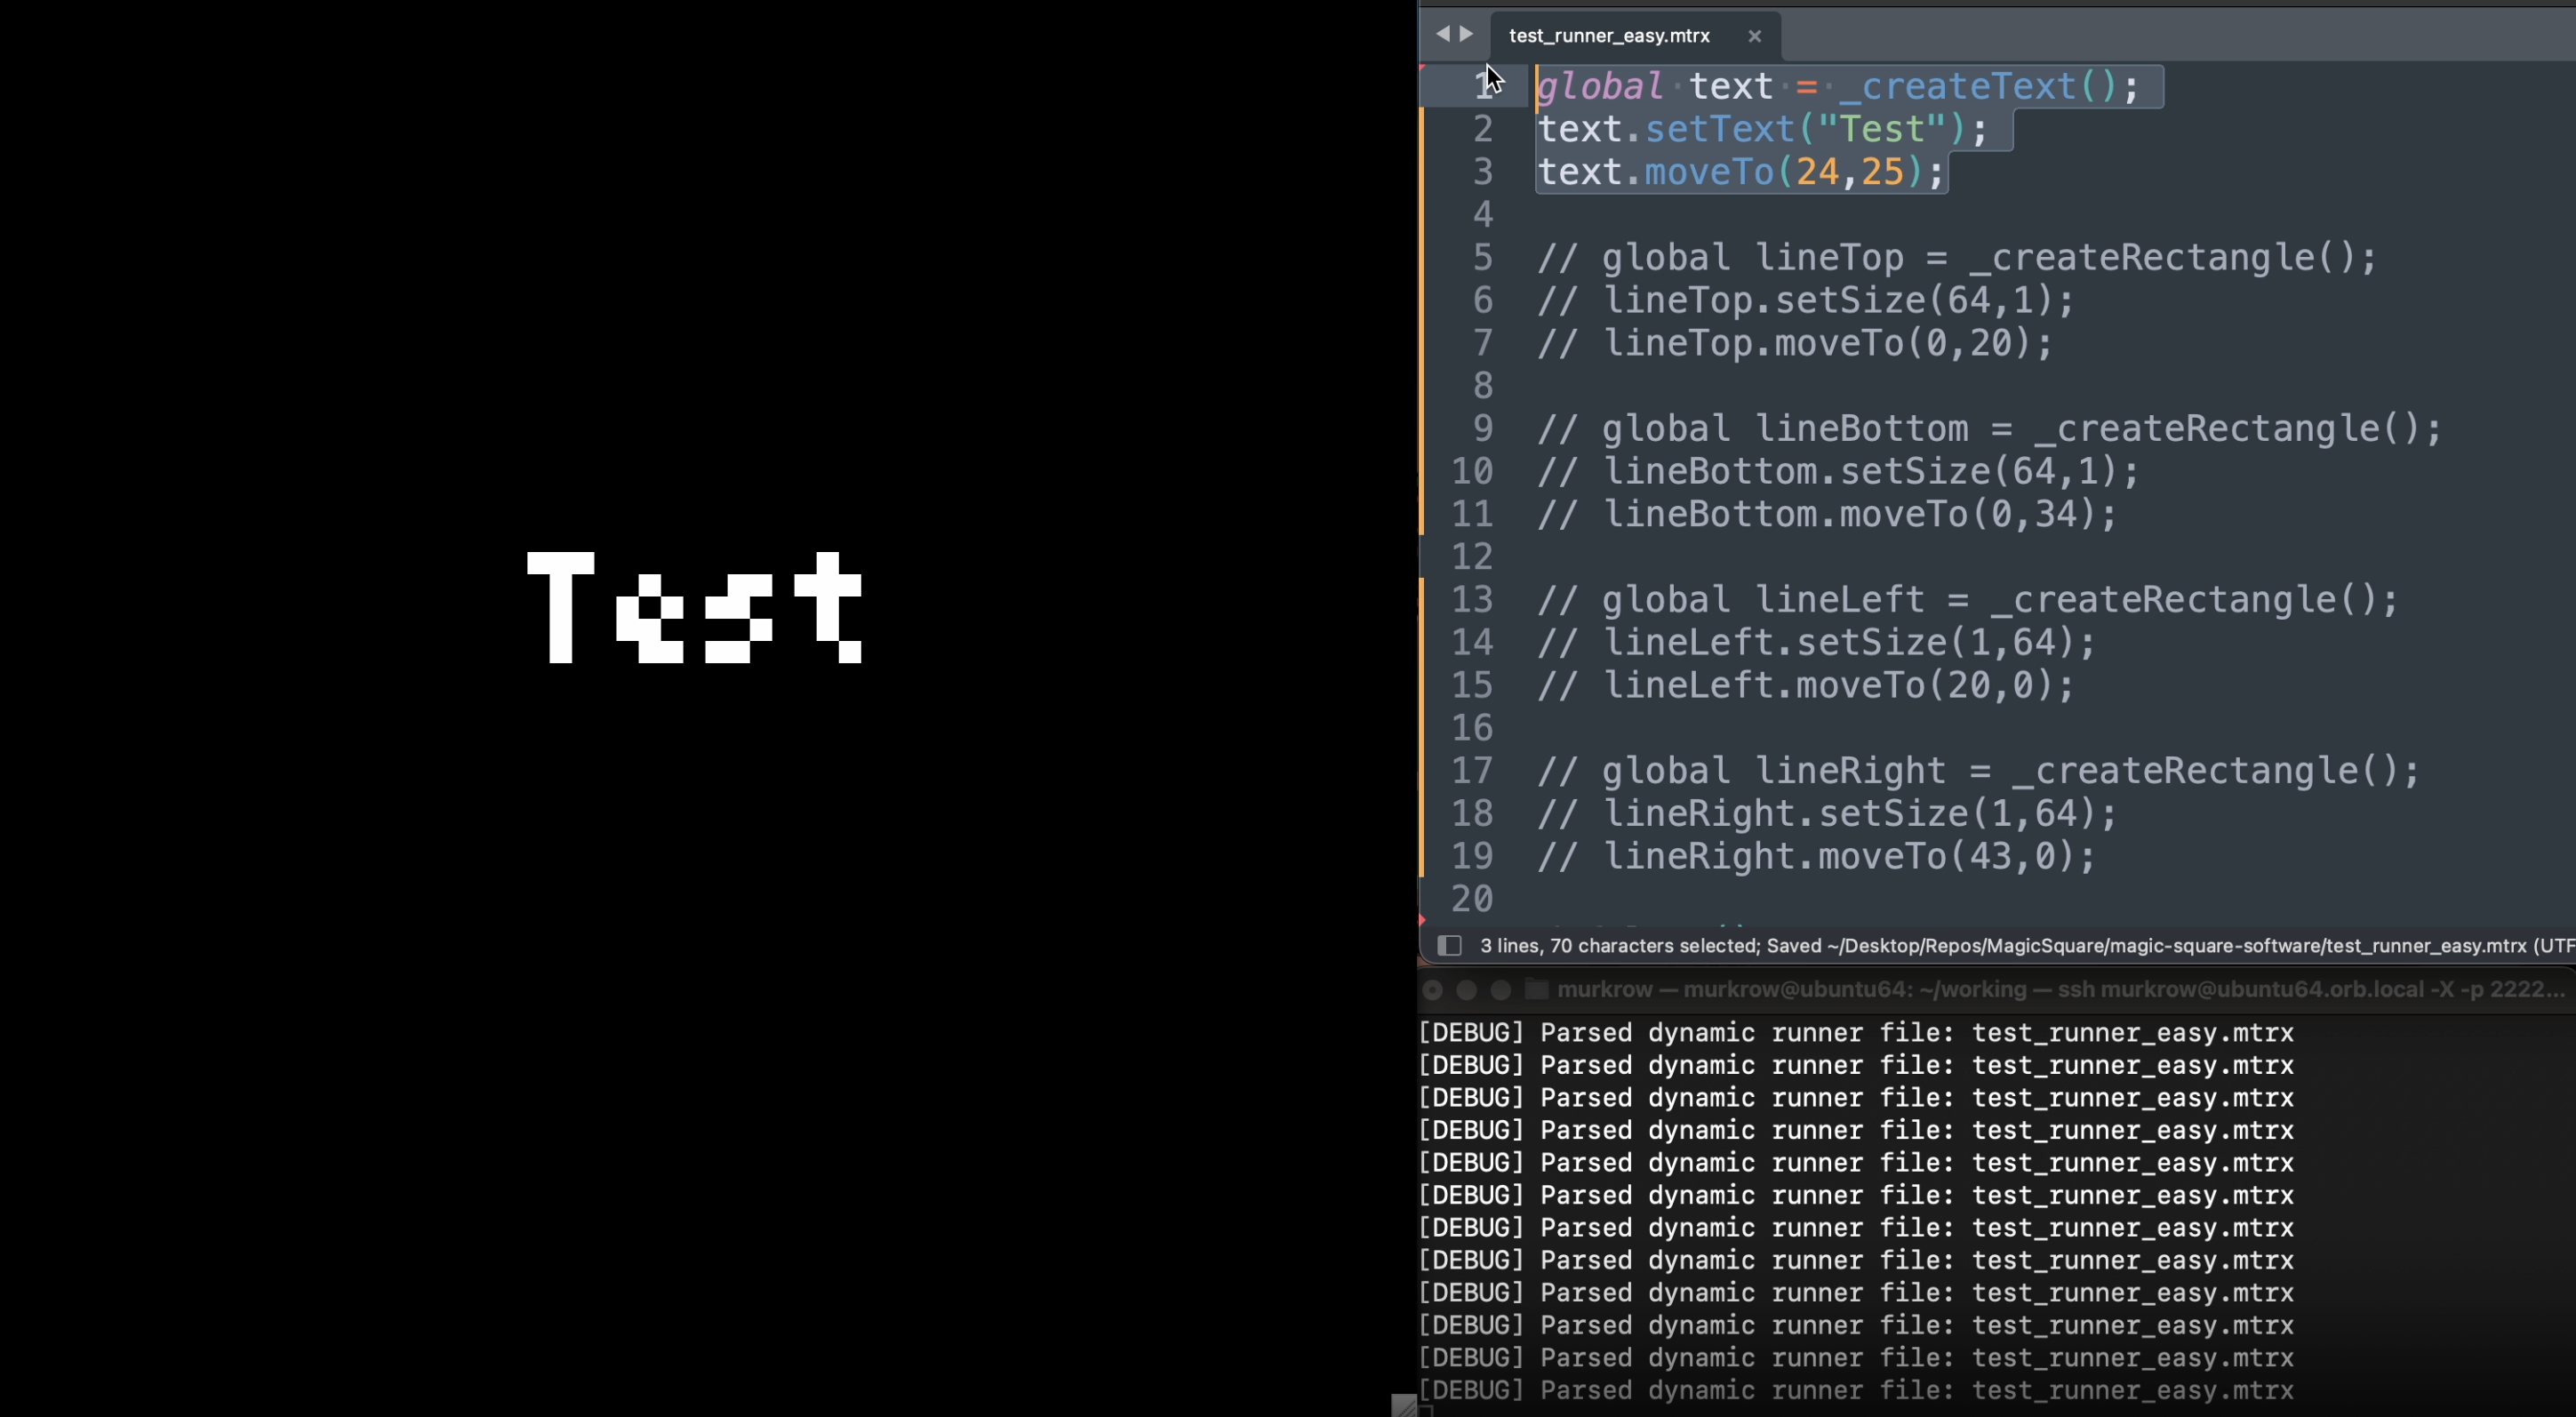
\includegraphics[width=\textwidth]{tesi/img/chai_demo/1.png} \caption*{Creation of a Text drawable} \end{minipage} \begin{minipage}[b]{0.49\textwidth} \centering 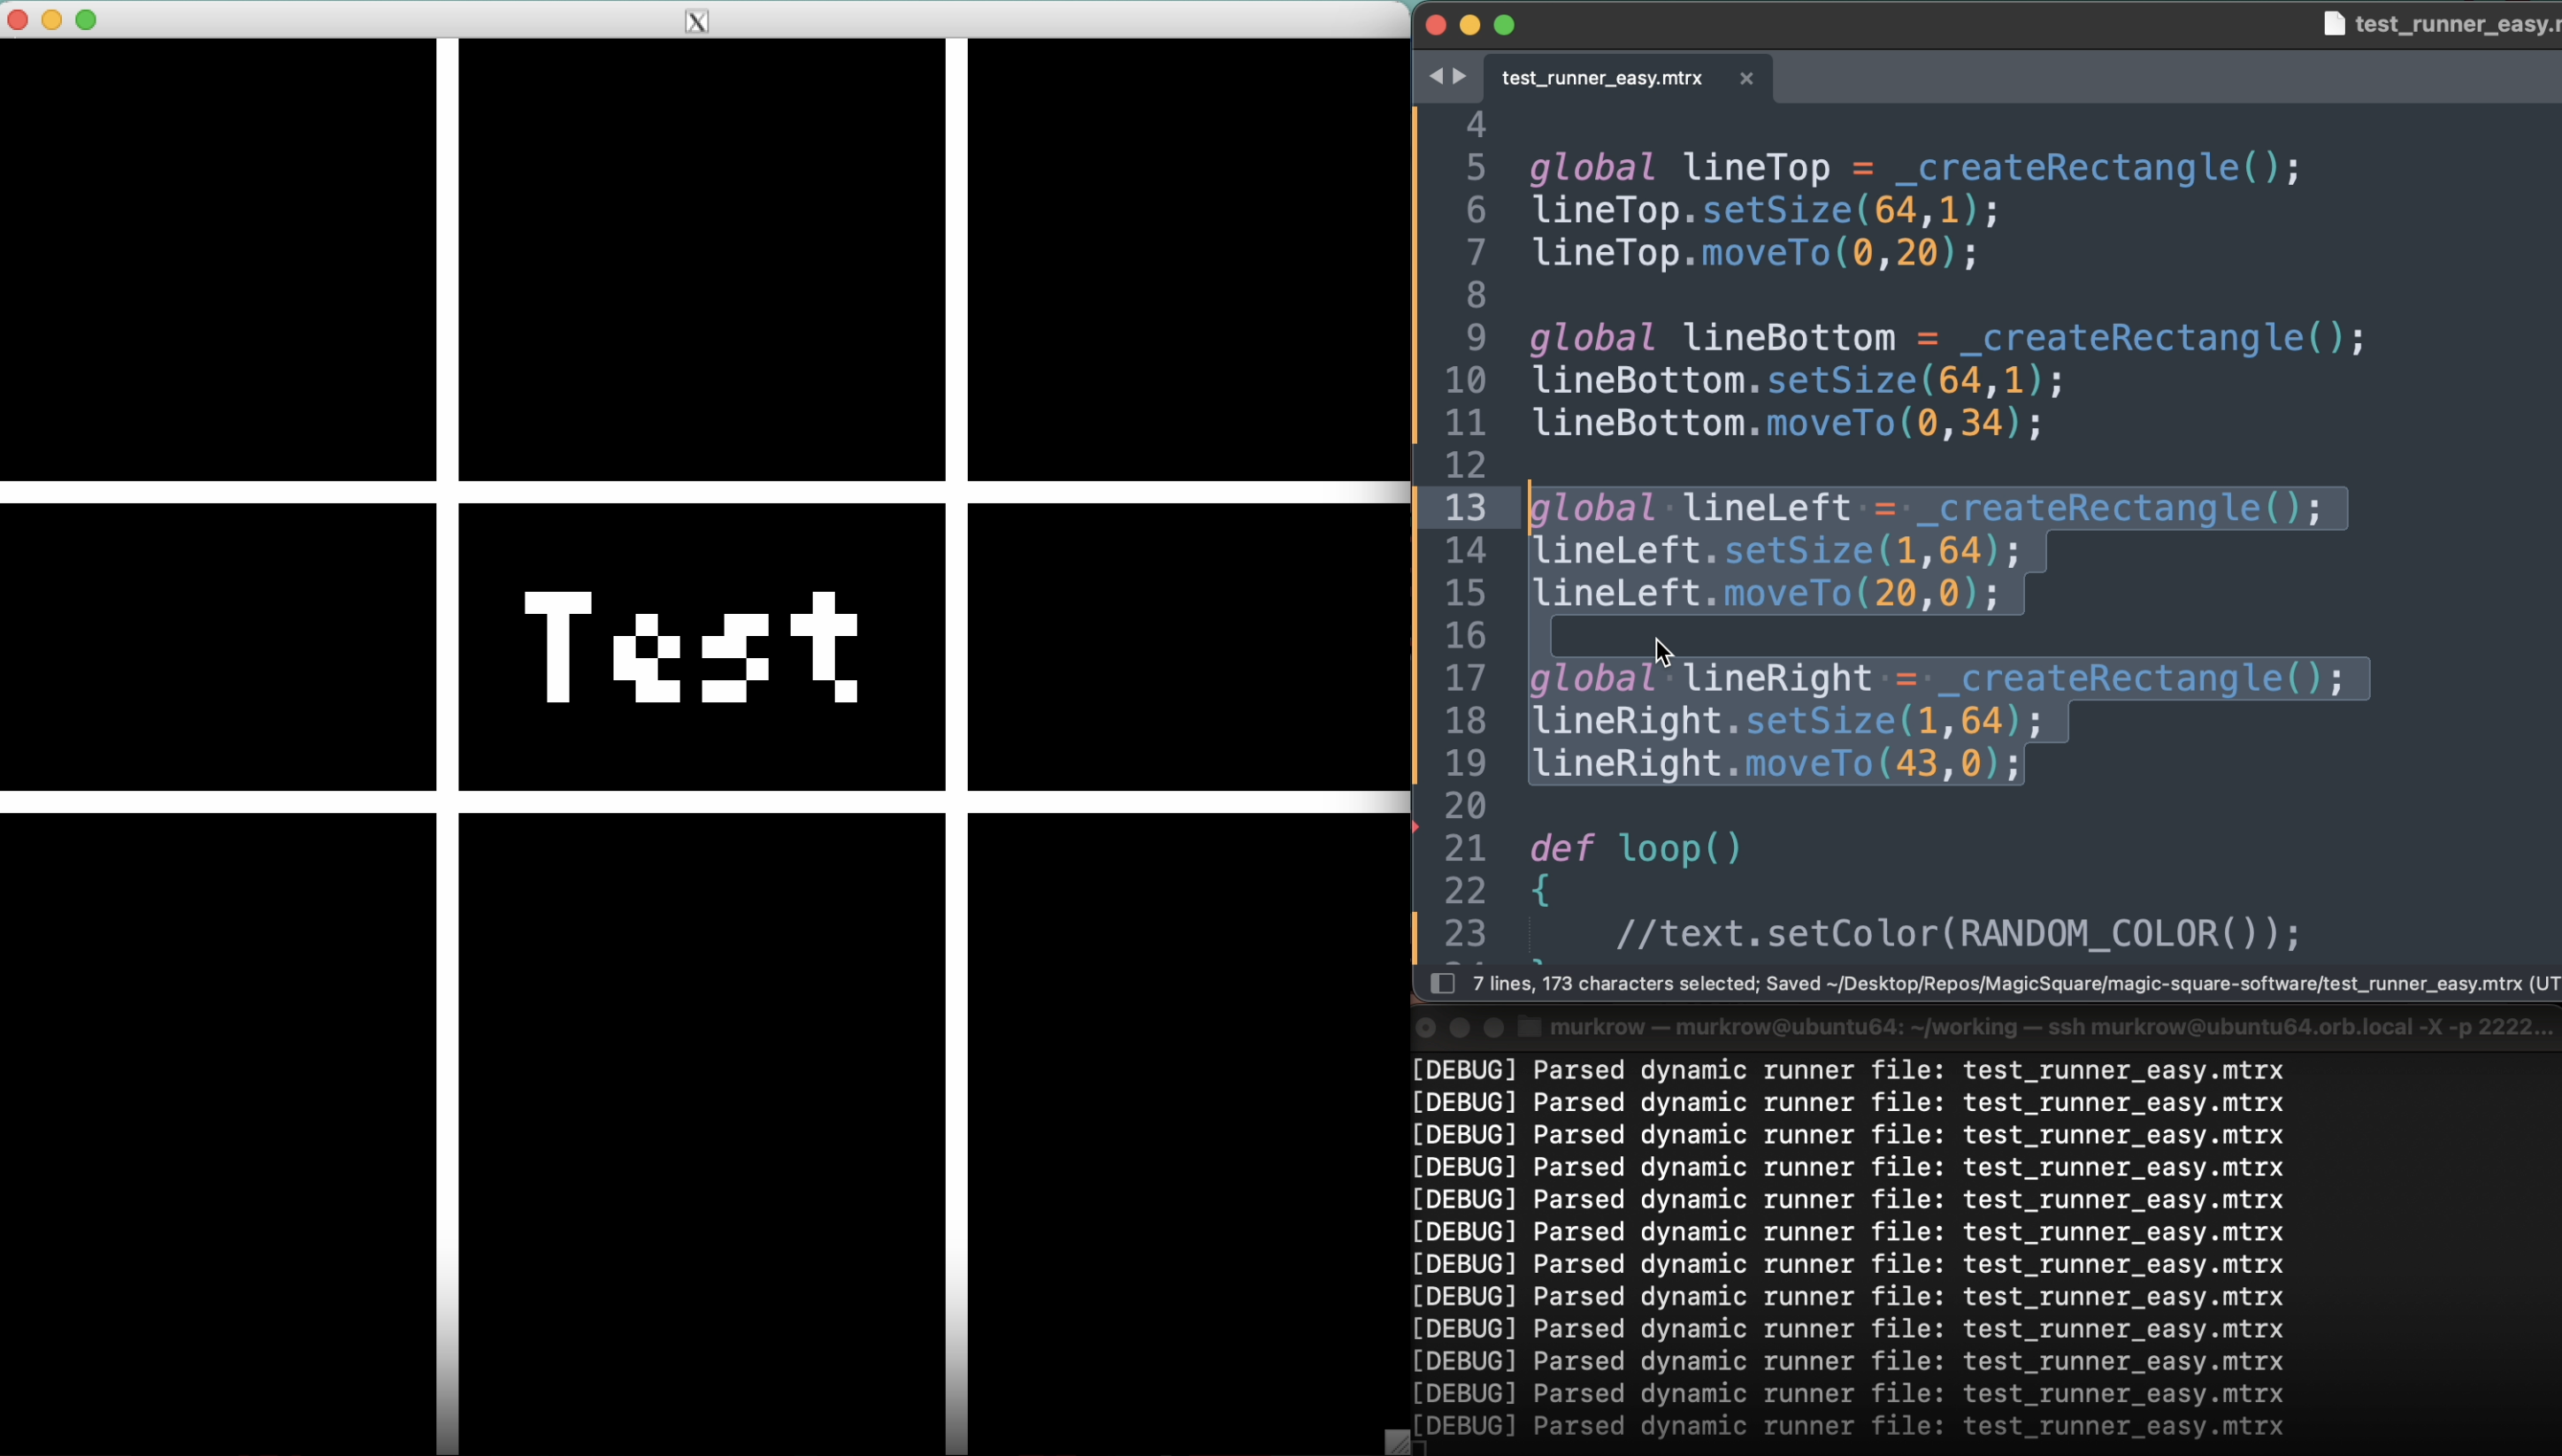
\includegraphics[width=\textwidth]{tesi/img/chai_demo/2.png} \caption*{Creation of 4 rectangles} \end{minipage} \end{figure}

\begin{figure}[h] \centering \begin{minipage}[b]{0.49\textwidth} \centering 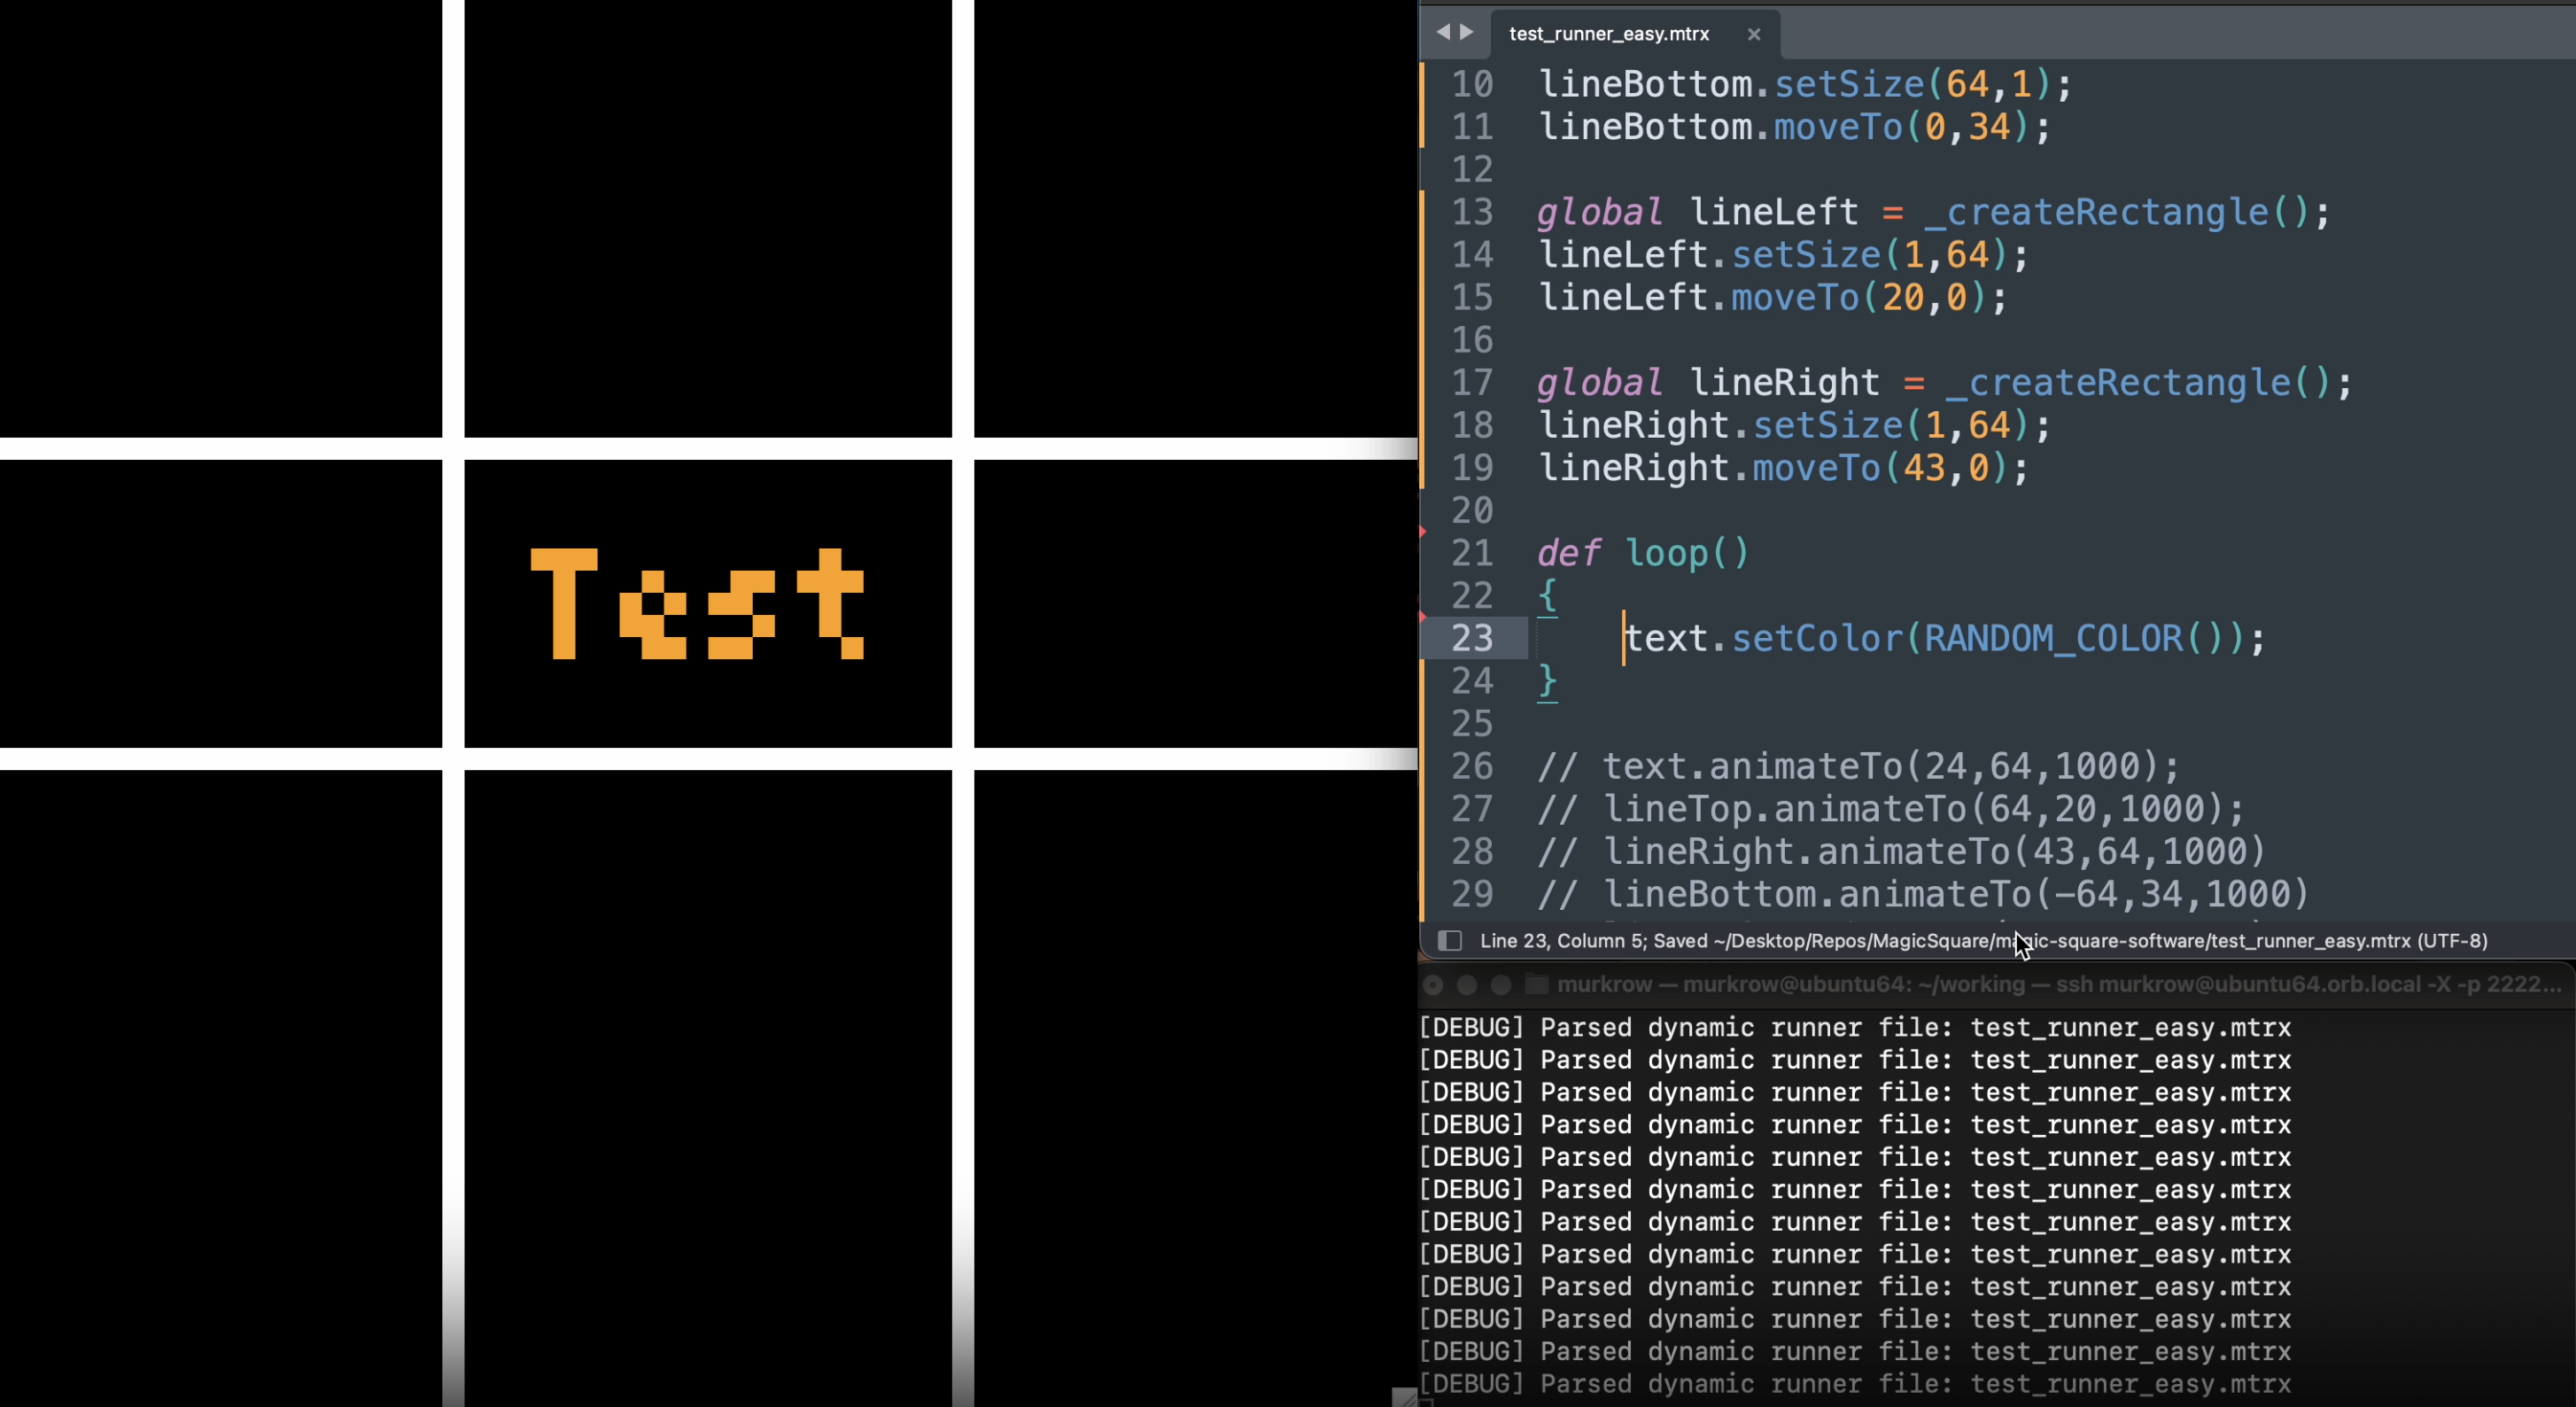
\includegraphics[width=\textwidth]{tesi/img/chai_demo/3.png} \caption*{Set text in random colors in the loop() function} \end{minipage} \begin{minipage}[b]{0.49\textwidth} \centering 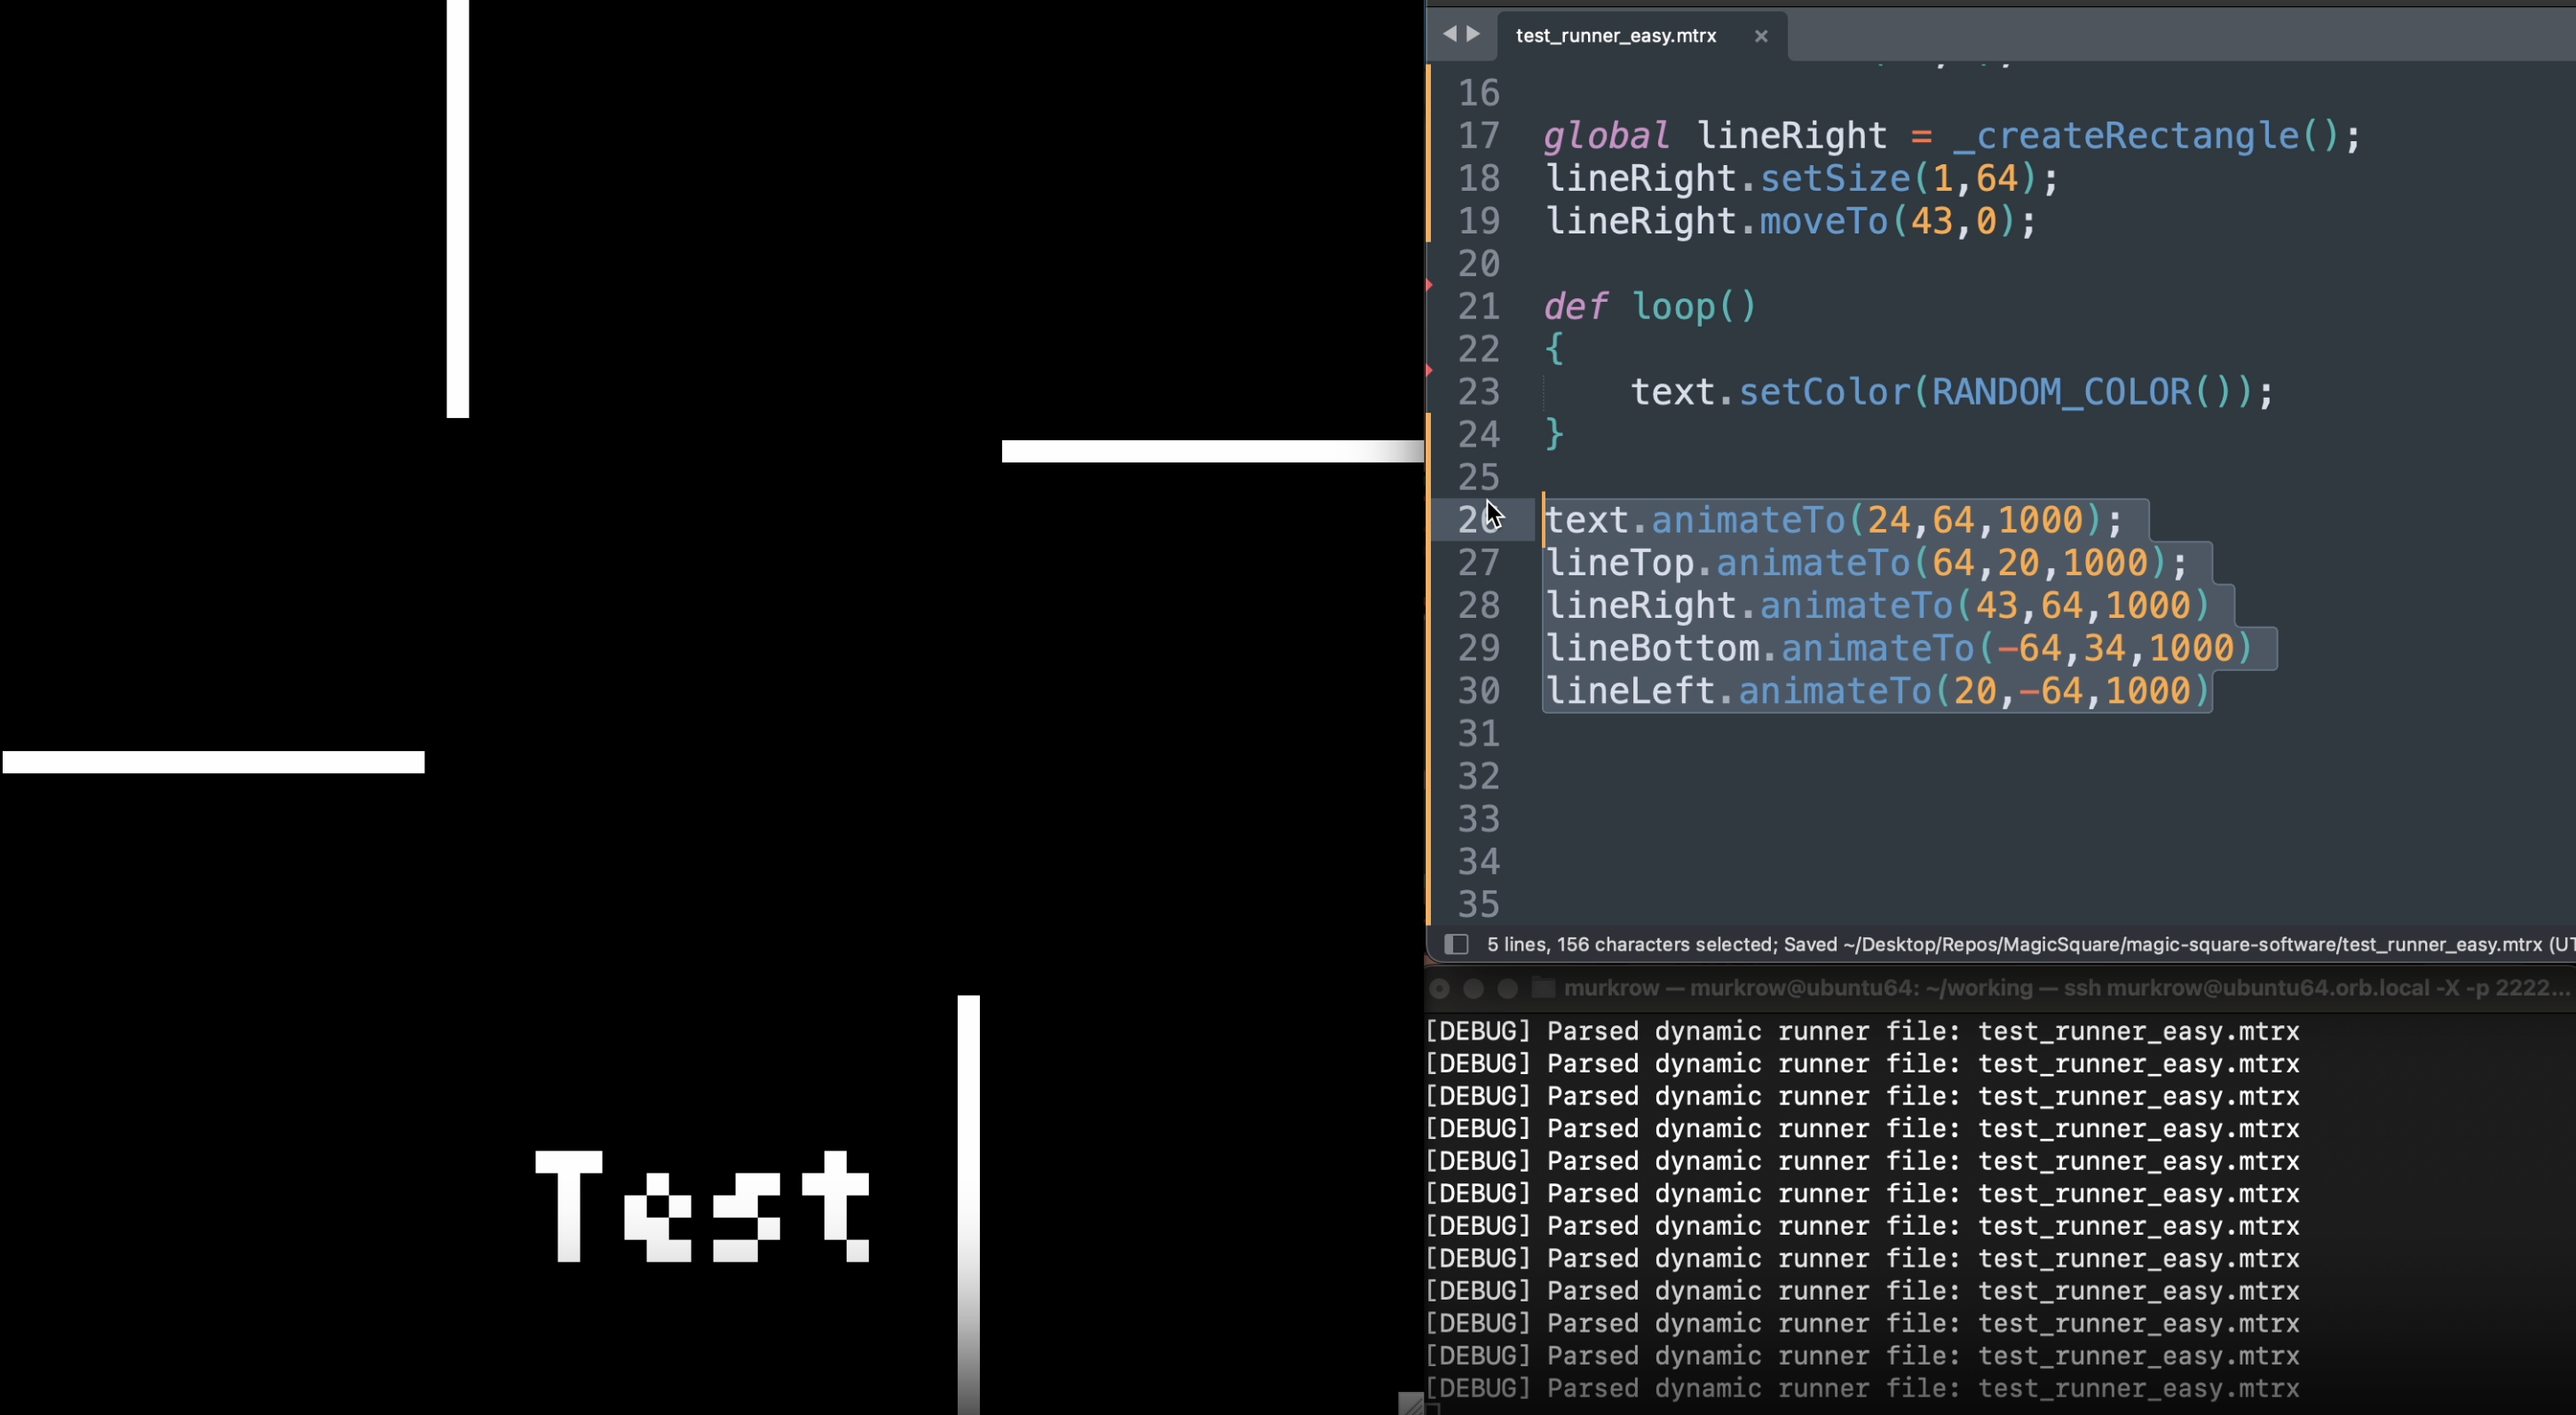
\includegraphics[width=\textwidth]{tesi/img/chai_demo/4.png} \caption*{Animate everything to fade away} \end{minipage} \end{figure}

This solution allowed the engine to interpret and render widgets in real-time, with no recompilation required—an exciting milestone!

\subsubsection{ChaiScript Limitations} While ChaiScript was a solid fit, I eventually realized its limitations:


\begin{itemize}
    \item \textbf{Language popularity}: The language is mostly straightforward and easy to use but is far from being popular. In fact, there are few resources online to learn how to use it, and it's not frequently updated.
    \item \textbf{Language modularity}: Chaiscript has no standard modules. While the community has created a few for tasks such as math functions and JSON deserialization, any additional functionality like a REST client or file management requires wrapping C++ libraries manually.
\end{itemize}


\subsubsection{Discovering Pybind11 and Python Integration} After further research, I discovered Pybind11 \cite{pybind11}, a library that enables seamless embedding of the Python interpreter within C++ code. Despite my initial reservations about Python, its vast modularity—achieved through pip packages—and its popularity made it an attractive alternative to ChaiScript.

With Pybind11, mapping C++ classes to Python objects is nearly effortless, requiring only minimal class declarations. This allowed me to tap into Python's full power while maintaining the performance and flexibility of my C++ engine.


\begin{minted}{c++}
PYBIND11_EMBEDDED_MODULE(mosaico, m) {

    // Bind color class
    py::class_<Color>(m, "Color")
    .def(py::init<int, int, int>());

    // Binding the MatrixWidget class
    py::class_<MatrixWidget>(m, "MatrixWidget")
            .def("createRectangle", &MatrixWidget::createRectangle)
            .def("createImage", &MatrixWidget::createPPM)
            .def("createText", &MatrixWidget::createText)
            .def("createCanvas", &MatrixWidget::createCanvas)
            .def("remove", &MatrixWidget::unregisterDrawable)
            .def("setPixel", &MatrixWidget::setPixel)
            .def("clear", &MatrixWidget::clearDrawables);

    // Bind the Drawable class
    py::class_<Drawable>(m, "Drawable")
    .def("moveTo", &Drawable::moveTo)
    .def("translateBy", &Drawable::translateBy)
    .def("translateXBy", &Drawable::translateXBy)
    // a lot of other stuff
}
\end{minted}

\newpage

The last thing to do is to create a \textit{DynamicWidget} class that will inherit from \textit{Widget} and will invoke the python script to get a new canvas each frame or to register drawables:

\begin{minted}{c++}

class DynamicWidget : public MatrixWidget {
public:
    DynamicWidget(std::string widgetPath, std::string configurationPath){
        // Get files from path and parse metadata
        if (!initializePaths() || !readMetadata()) {
            validWidget = false;
            Logger::logError("Widget initialization failed");
        } else {
            validWidget = true;
            Logger::logDebug("Widget loaded successfully");
        }
        // Register C++ -> Python bindings
        bindObjectsToPython();
        // Load the widget script and execute everything except the loop function
        py::exec(widgetScriptString);
    }
        void renderNextFrame(Canvas* canvas) override {
        try {
            // Execute the loop function
            py::exec("loop()");
        } catch (const py::error_already_set &e) {
            Logger::logError("Error while executing loop function: " + std::string(e.what()));
            validWidget = false;
            canvas->Fill(RED_COLOR);
        }
    }
}
\end{minted}

\newpage

\subsection{Canvas buffer}
The prototype now seems quite ready but there is a single problem left: every widget, even if as far as it is concerned is writing on a \textit{Canvas}, it is still using the real matrix under the hood to render pixels, this can cause problems for scenarios like this:

\begin{minted}{c++}
// Main loop
while (true) {
    matrix->clear();
    // Matrix is full black here
    veryComplexWidget->renderNextFrame(matrix); // will write pixel by pixel
    // Content is now displayed
}
\end{minted}

It is obvious that writing single pixels directly on a matrix is a problem for widgets that requires a bit of computation between pixel and pixel and will result in image flickering.
Luckily the library I used provided me two useful methods:

\begin{minted}{c++}
  // Create a new buffer to be used for multi-buffering. The returned new
  // Buffer implements a Canvas with the same size of thie RGBMatrix.
  // You can use it to draw off-screen on it, then swap it with the active
  // buffer using SwapOnVSync(). That would be classic double-buffering.
  //
  // You can also create as many FrameCanvas as you like and for instance use
  // them to pre-fill scenes of an animation for fast playback later.
  FrameCanvas *CreateFrameCanvas();

  // This method waits to the next VSync and swaps the active buffer with the
  // supplied buffer. The formerly active buffer is returned.
  FrameCanvas *SwapOnVSync(FrameCanvas *other, unsigned framerate_fraction = 1);
\end{minted}

By incorporating these methods into the code, I effectively resolved the flickering issue. This approach enabled smooth rendering by leveraging double-buffering, ensuring that complex widgets could perform the necessary computations without directly writing pixels to the matrix, thus eliminating visual artifacts.

\newpage

I then decided to separate a bit of concerns and I started working on a \textit{CanvasBuffer} class. Since my intent was not to write on the real matrix anymore but to create a set of canvas to swap on the matrix at some point in time, I also seized the occasion to make these canvases even more generic by giving them the possibility to be of arbitrary sizes, they still needed to be smaller than the hardware matrix itself but they could occupy for example the bottom half of the screen, the top left quarter etc. I called this class \textit{CanvasLayer} and it looks like this:

\begin{minted}{c++}
/// A CanvasLayer is a layer that can be painted on by a widget.
/// Allows to create composite widgets to be displayed on the matrix.
/// Can be narrower or shorter than the matrix.
class CanvasLayer : public Canvas {

private:

    // Pixels are stored in a list to allow for 
    // easy iteration and manipulation
    std::list<Pixel> pixels;

public:

    CanvasLayerPosition pos;
    CanvasLayer(CanvasLayerPosition position = CanvasLayerPosition::FULL);
    ~CanvasLayer();

    // Will actually write pixels on another canvas (even the matrix)
    void paintOntoCanvas(Canvas *canvas, int xOff = 0, int yOff = 0);
    int width() const;
    int height() const;
    void Fill(Color color);
    void SetPixel(int x, int y, Color color);
    void Clear();
    CanvasLayer *Clone();
    void setBorder(Color color);
    void setPadding(int padding);
    int getPixelCount();
};
\end{minted}

\newpage

As you may notice, the \textit{CanvasLayer} class simply implements the \textit{Canvas} interface. The principle of dependency inversion mentioned before \ref{widget_canvas_abstraction} allowed me to do this upgrade while being completely transparent to objects that worked with a \textit{Canvas}.

This is what the \textit{CanvasBuffer} class looked like:


\begin{minted}{c++}

/// This class is responsible for buffering the canvas frames
/// This is useful when you want to render multiple widgets on the matrix and be able to show them all at once
/// The buffer will be able to swap the frames on the matrix without flickering
class CanvasBuffer {

private:
    MatrixDevice *matrix;
    std::list<Canvas*> buffer;

public:
    CanvasBuffer(MatrixDevice *matrix, int bufferSize) {
        this->matrix = matrix;
        for (int i = 0; i < bufferSize; i++) {
            buffer.push_back(matrix->CreateFrameCanvas());
        }
    }
    // This can be called multiple time for the current frame
    // Is basically used to compose the final composite frame
    // to later swap on the matrix using loadNextFrameOnMatrix()
    void paintPartialLayerOnCurrentFrame(CanvasLayer *canvasLayer) {
        auto *currentFrame = buffer.front();
        canvasLayer->paintOntoCanvas(currentFrame);
    }
    // Uses the frame crafted with the method above to swap it on actual matrix
    void loadNextFrameOnMatrix() {
        // Swap current frame on matrix
        auto *currentFrame = buffer.front();
        buffer.pop_front(); 
        matrix->SwapFrameCanvas(currentFrame); 
        buffer.push_back(currentFrame); 
        // Prepare next frame
        auto *nextFrame = buffer.front();
        nextFrame->Clear();
    }
};
\end{minted}

\newpage
This is the high-level view of the whole final rendering software:

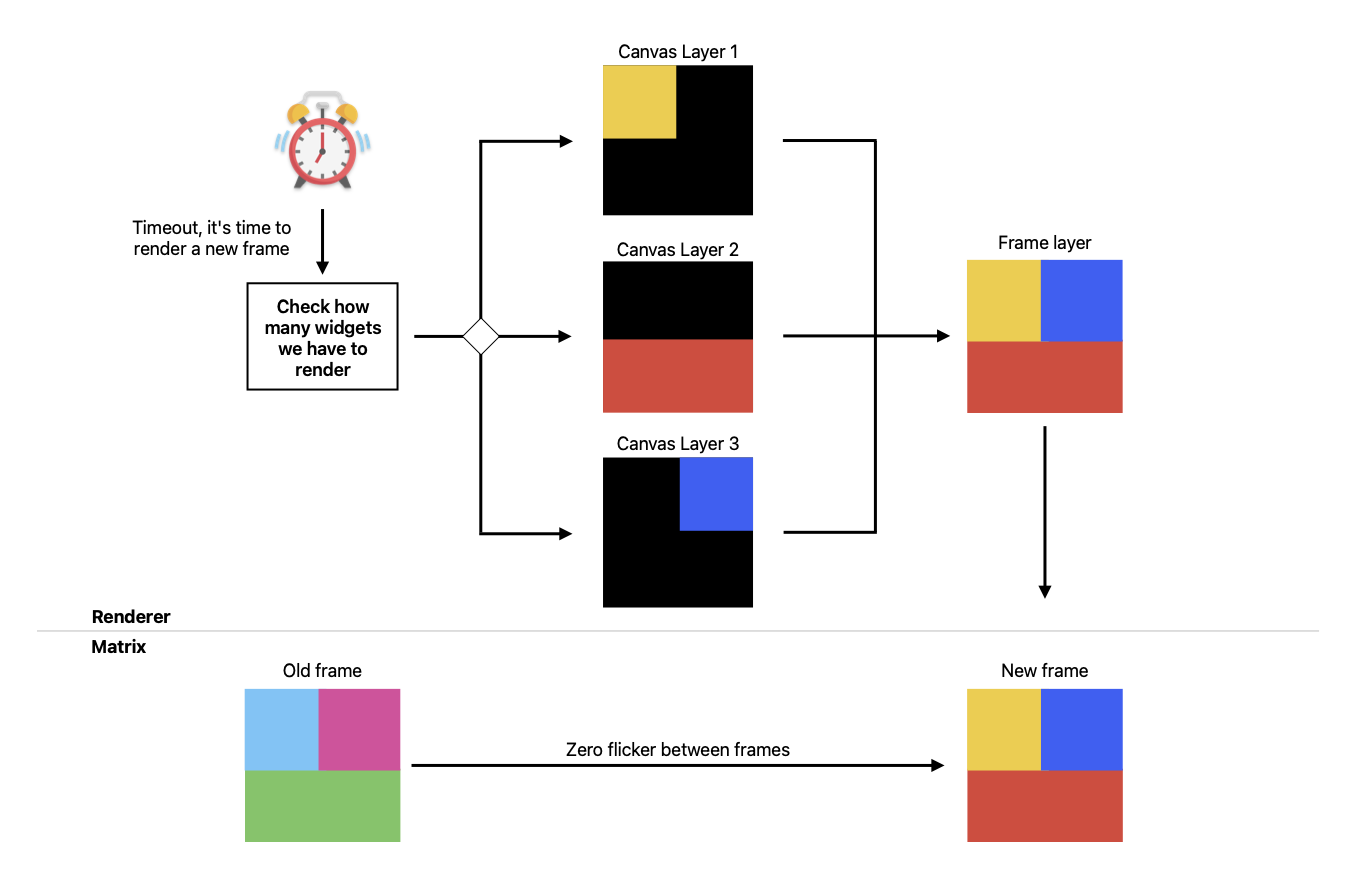
\includegraphics[width=\textwidth]{tesi/img/software-renderer.png}
\newpage
\section{Python Module}
Initially, my intention was to develop the entire software in C++. However, it became evident that a significant amount of time was being wasted on implementing basic functionalities, such as making remote API calls, deserializing JSON objects, or managing simple data in a local SQLite database.

As I have grown accustomed to working with higher-level abstractions that facilitate productivity and enable the maintenance of clean, organized codebases, it became apparent that achieving similar levels of efficiency in C++—a language not primarily designed for such tasks—was considerably more challenging. 

The complexity escalated when I attempted to set up a BLE GATT (Bluetooth Low Energy Generic Attribute) server in C++. I discovered that no high-level abstractions existed for this purpose in any of the available C++ libraries. In contrast, I found an easy-to-use and powerful Python library called \textit{Bless}\footnote{\url{https://pypi.org/project/bless/}}.

This realization led me to a pivotal decision: to shift the networking and data management logic from C++ to Python, thereby leveraging Python's simplicity and robust ecosystem. This move allowed the C++ module to focus on a single, well-defined responsibility: rendering pixels and handling graphics efficiently.

The Python module is designed to serve three primary purposes:
\begin{itemize}
    \item Enable auto-discovery of the matrix for the client application via BLE.
    \item Establish a lightweight LAN COAP server to receive and process commands from the client app.
    \item Manage persistent data, such as user-specified widget configurations using a simple relational SQLite database.
\end{itemize}

\newpage
To facilitate communication between the C++ and Python modules, I implemented a Unix socket, allowing seamless inter-process communication between the two languages.

This is a complete specification of the possible commands that the COAP server can receive:

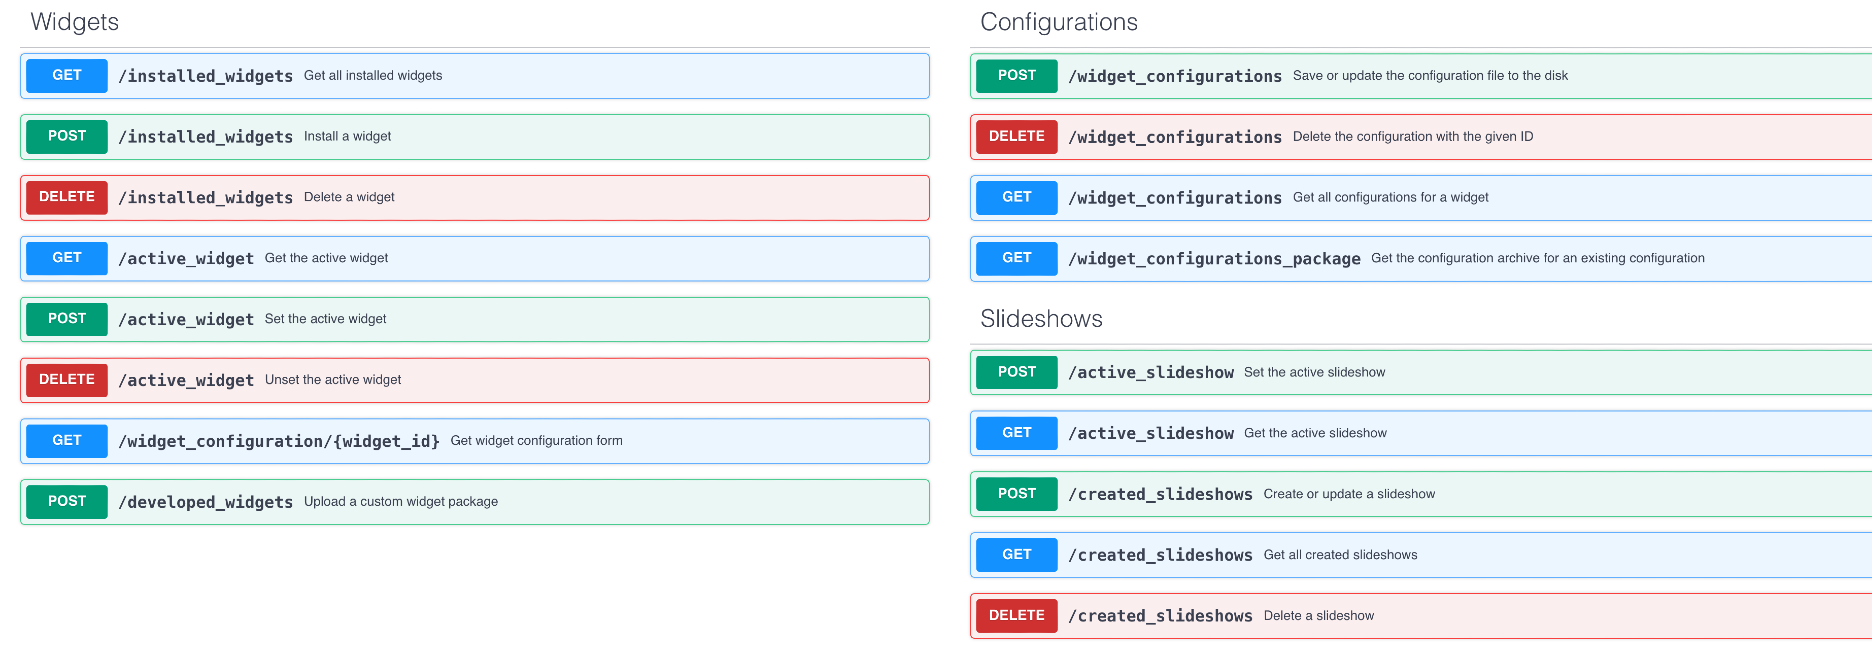
\includegraphics[width=1\textwidth]{tesi/img/coap-swagger.png}

This is an example interaction between the user, the app, the Python module and the C++ module:

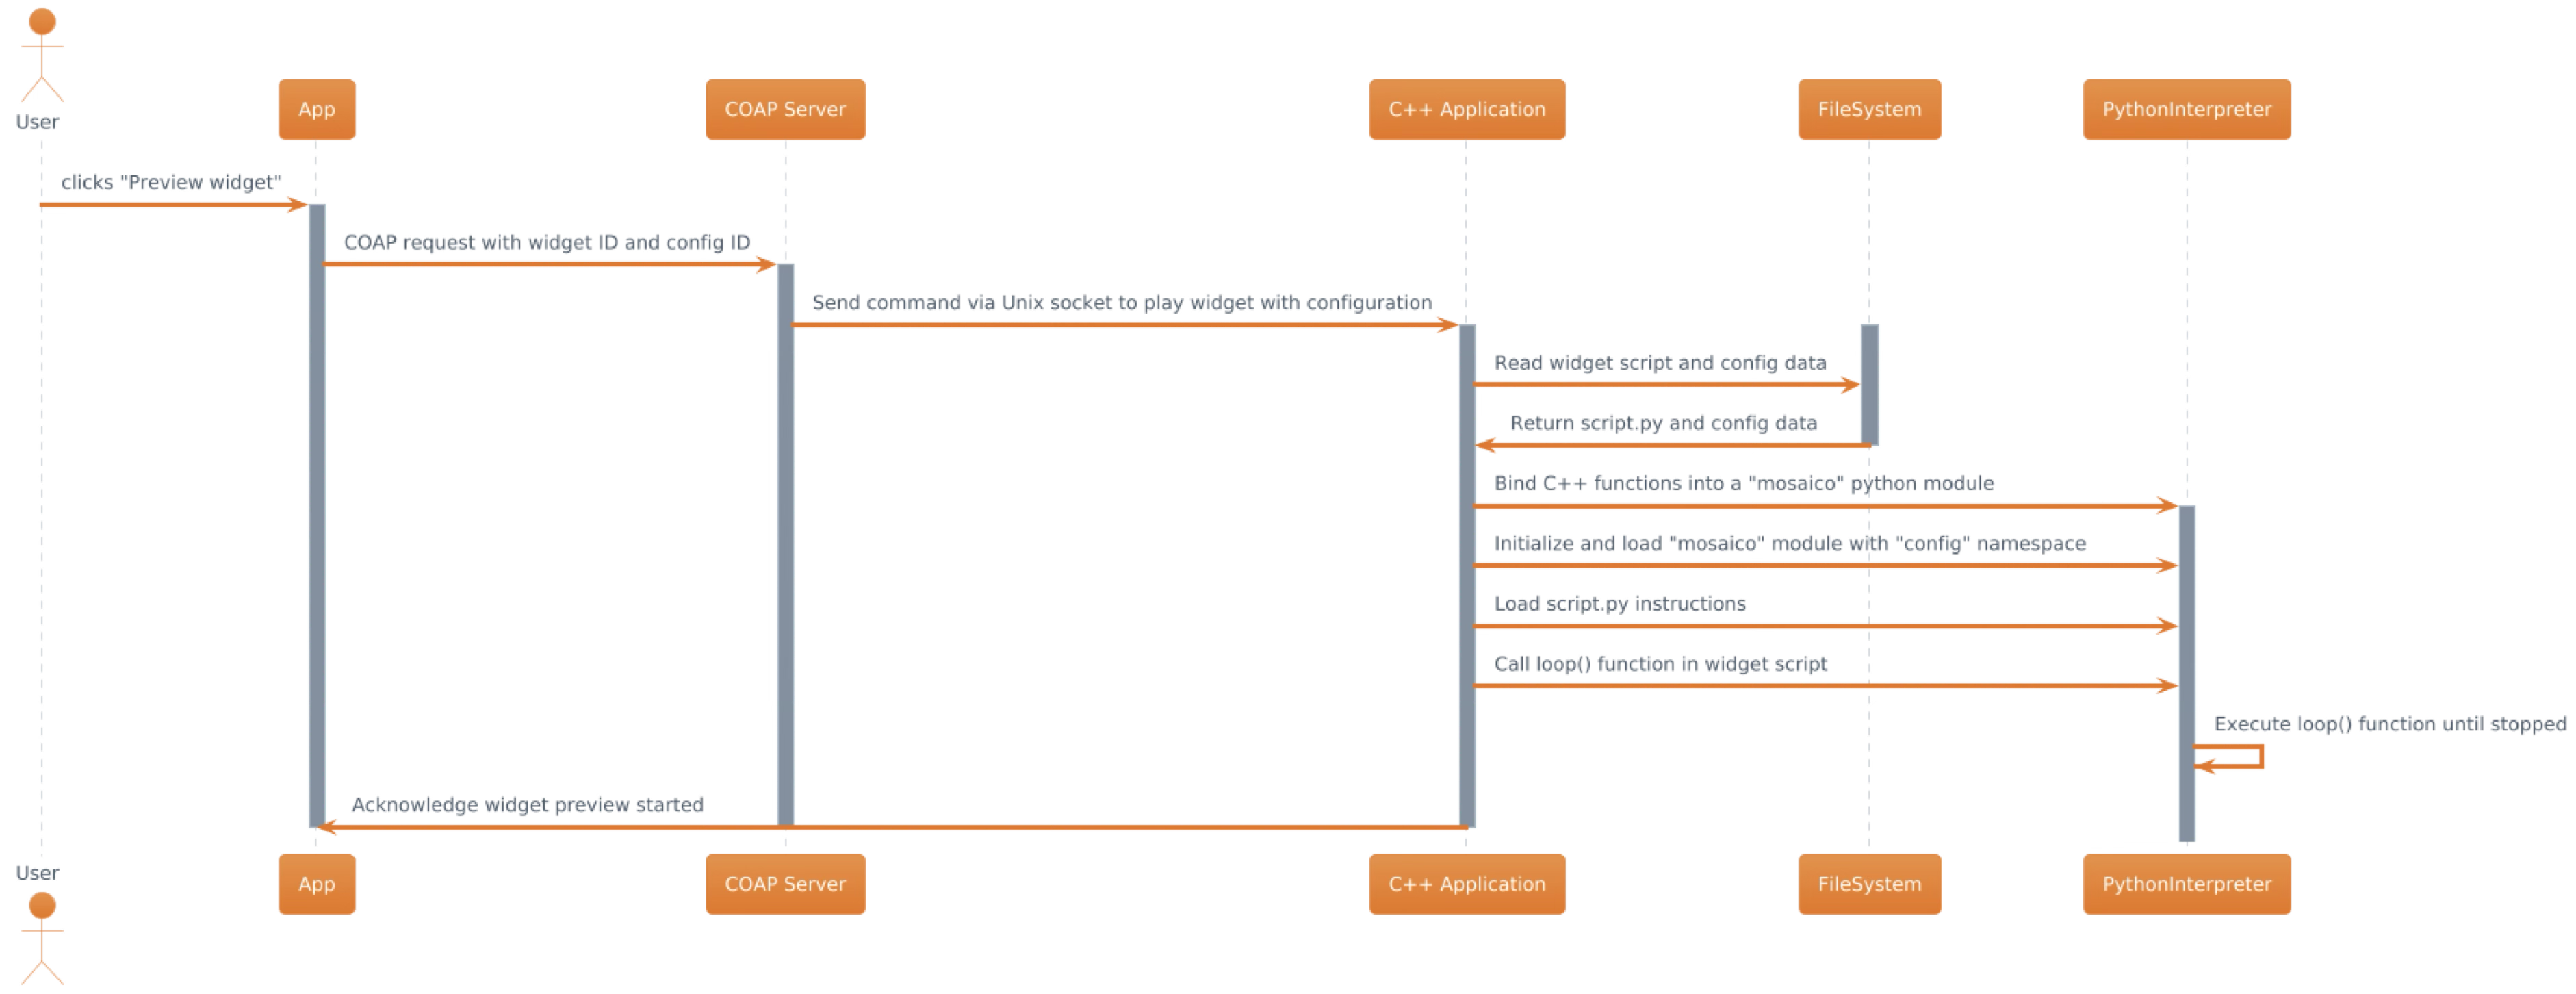
\includegraphics[width=1\textwidth]{tesi/img/activity-install-widget.png}
\newpage
\section{Cross Compiler}
One of the more challenging aspects of developing a complex C++ application is the creation of a makefile that accurately links all required modules and libraries. This challenge becomes even more pronounced when targeting a different architecture, as in the case of compiling for the ARMv6 CPU of the Raspberry Pi Zero W.

Compiling directly on the Raspberry Pi proved impractical, as each compilation took between 10 to 20 minutes to generate an executable—an unacceptable delay for iterative development. 

After extensive experimentation, I successfully identified a working cross-compilation toolchain tailored to the ARMv6 architecture \footnote{\url{https://github.com/tttapa/docker-arm-cross-toolchain/}}. This discovery significantly optimized the build process, reducing compile times to less than a minute. To streamline the development workflow, I created a Bash script that automates the compilation, establishes an \textit{SSH} connection to the Raspberry Pi, and uses \textit{rclone} to swiftly transfer the build artifacts to the device before launching the application.

Though this setup took considerable time to establish, it drastically accelerated the development process, allowing for rapid testing and debugging on the Raspberry Pi.

\newpage
\section{Simulators}
\label{simulators}
\begin{figure}[h]
 \centering
 \begin{minipage}[b]{0.32\textwidth}
    \centering
    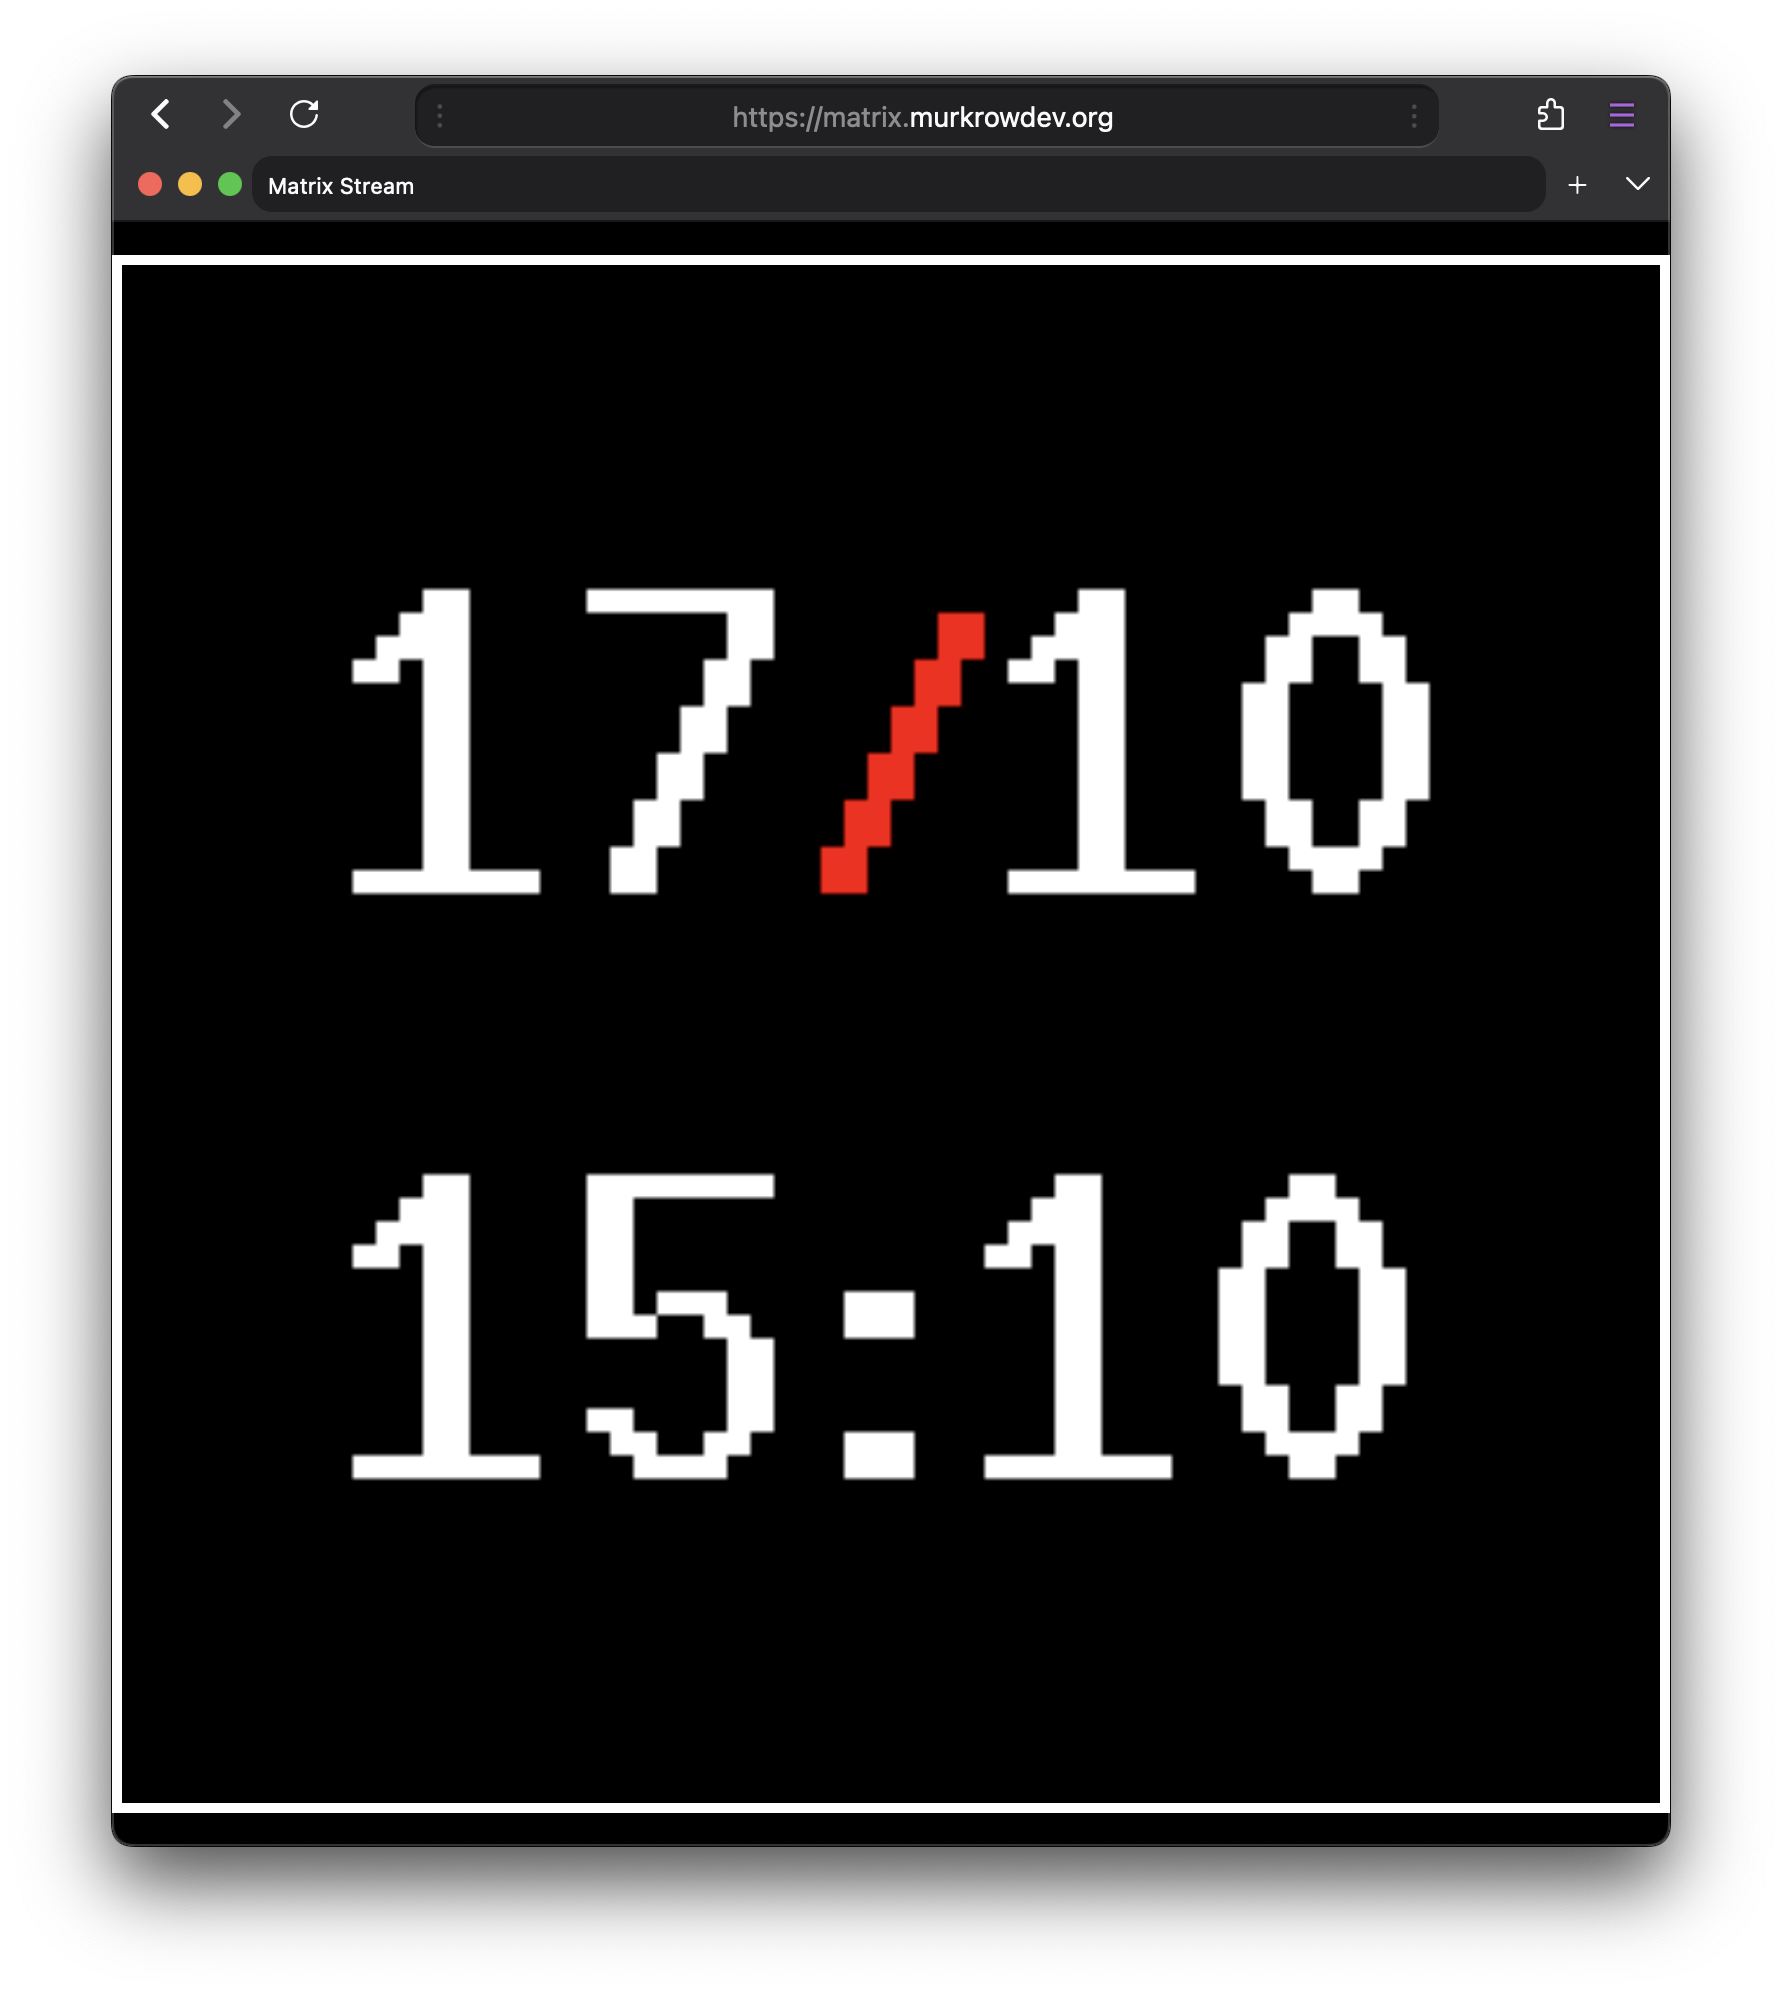
\includegraphics[width=\textwidth]{tesi/img/matrices/web.png}
    \caption*{Web simulator}
\end{minipage}
    \centering
    \begin{minipage}[b]{0.32\textwidth}
        \centering
        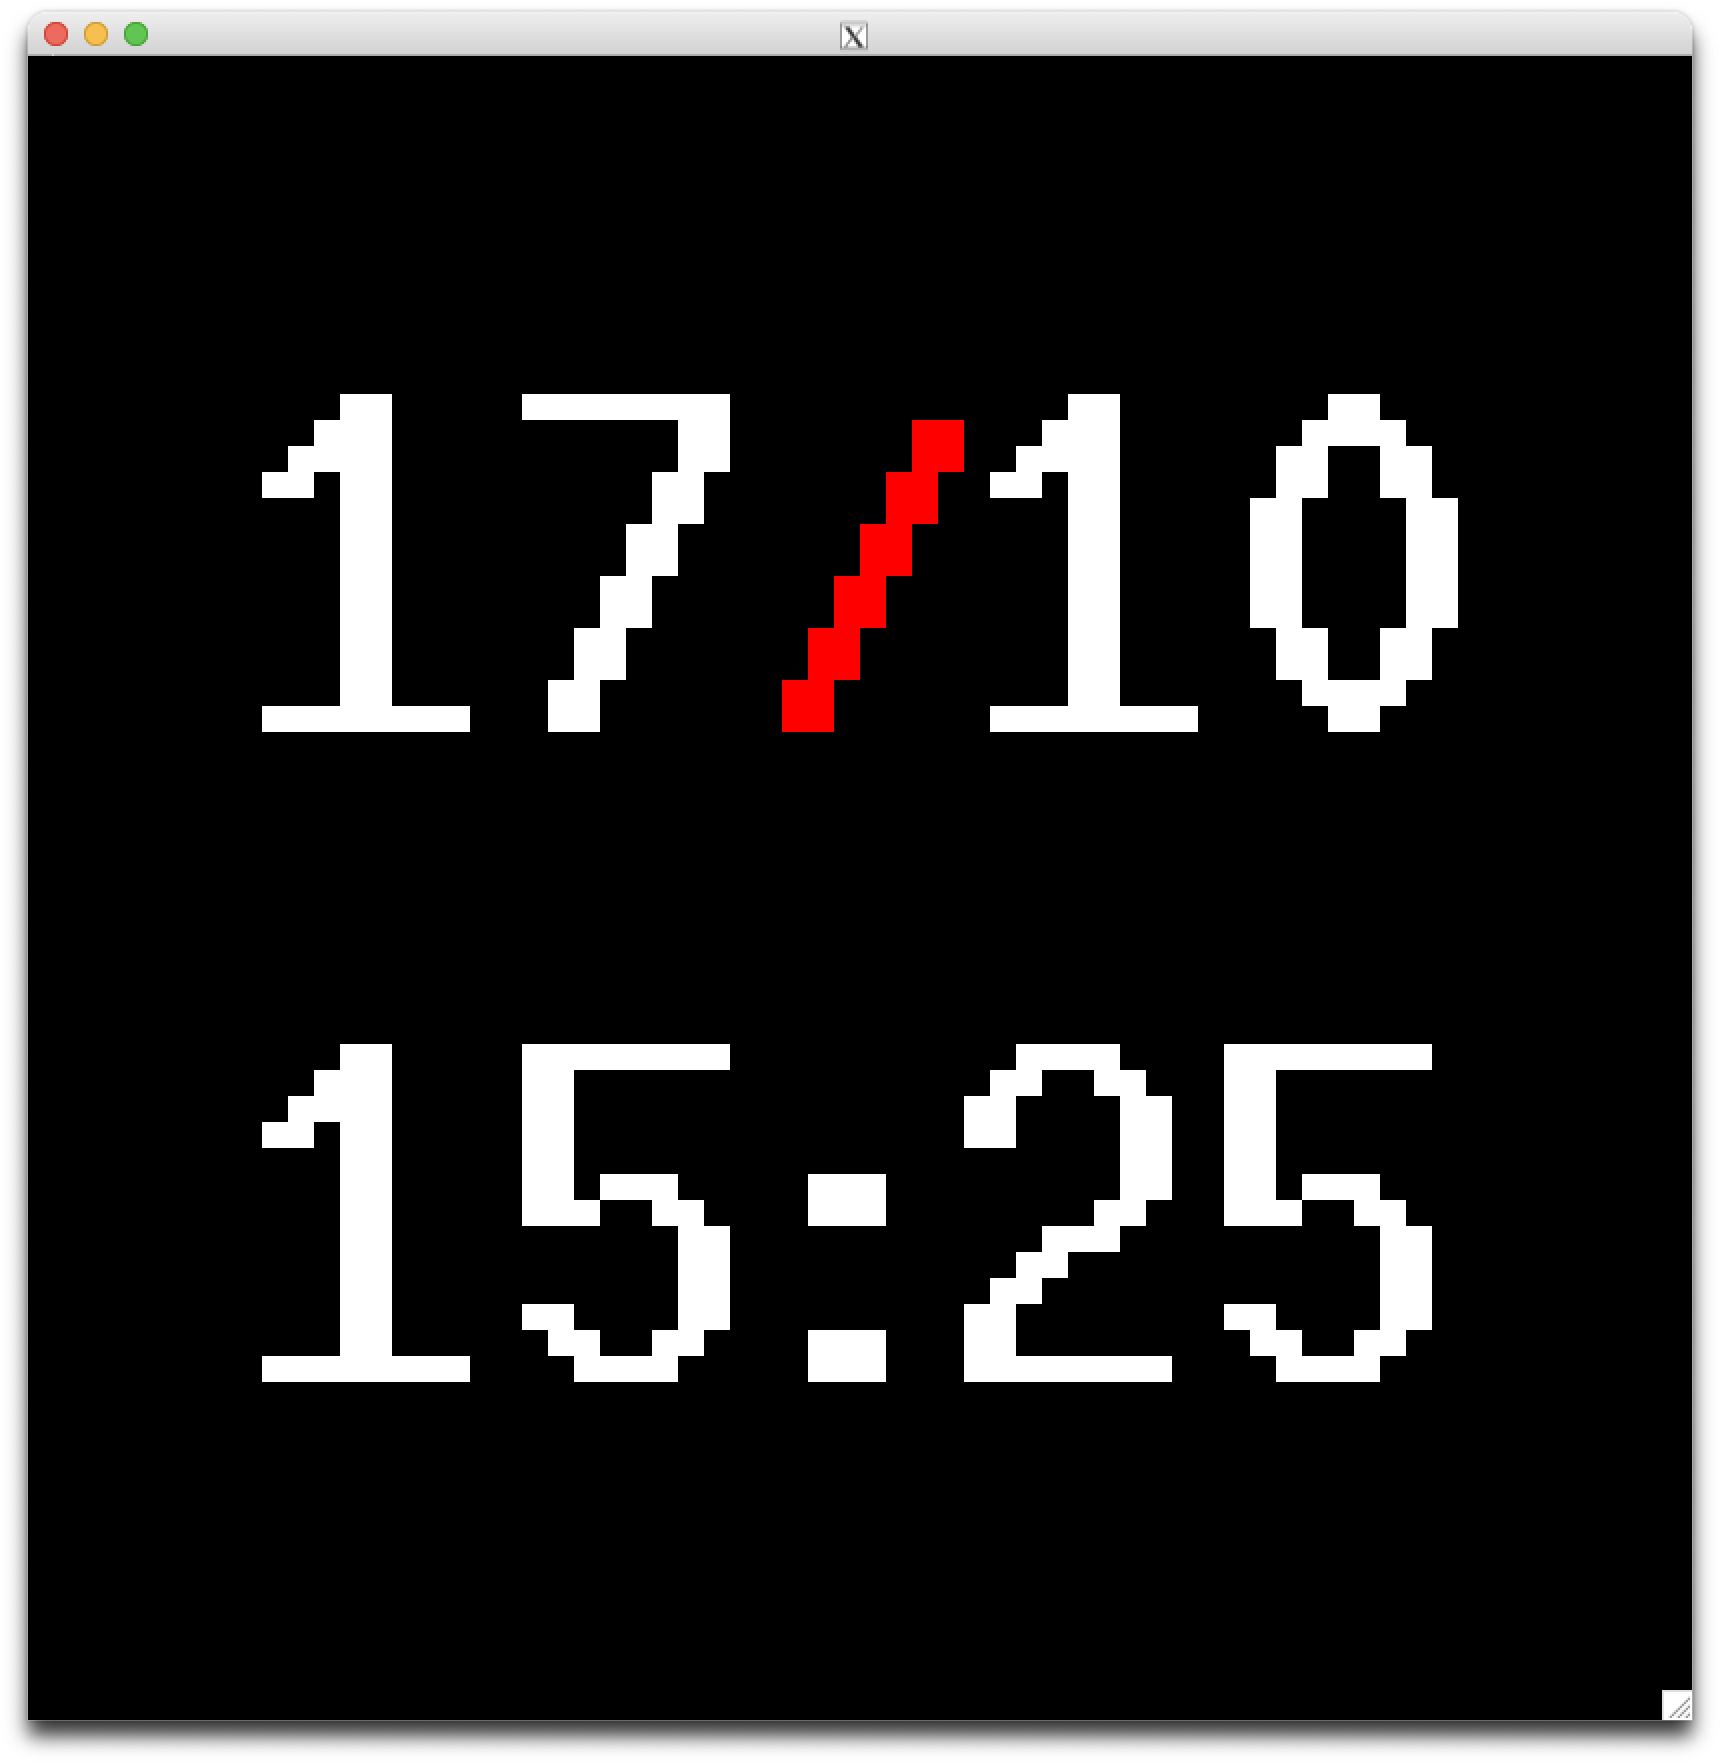
\includegraphics[width=\textwidth]{tesi/img/matrices/x11.png}
        \caption*{X11 windowed simulator} 
    \end{minipage}
    \centering
    \begin{minipage}[b]{0.32\textwidth}
        \centering
        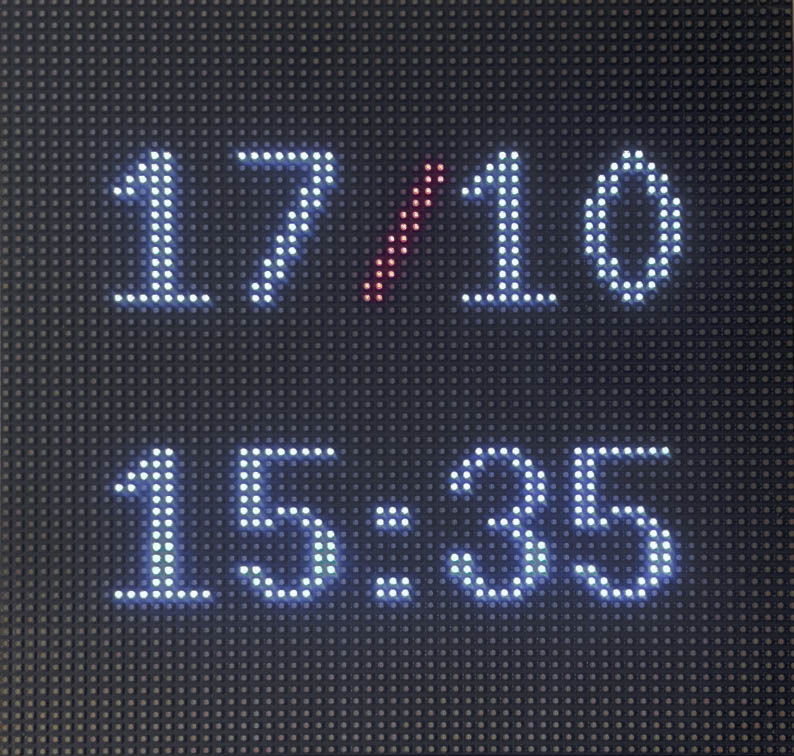
\includegraphics[width=\textwidth]{tesi/img/matrices/real.jpg}
        \caption*{Real matrix} 
    \end{minipage}
\end{figure}


Even with cross-compilers meticulously configured, the process of compiling and syncing files continued to be a significant drain on development time. Furthermore, given that I am frequently away from home, I sought a solution that would allow me to work on the project remotely, without the need for the physical hardware. Clearly, carrying the matrix and Raspberry Pi with me at all times was not a practical option. This led me to explore the idea of developing a matrix simulator from scratch.

Initially, the task appeared daunting, as I anticipated that a substantial amount of time and effort would be required to implement such a simulator. However, once again, the design principles employed throughout the application—particularly the use of dependency inversion—proved to be immensely beneficial.

One of the key architectural decisions in the project was to ensure that, aside from the application’s entry point, no other modules would have direct knowledge of the matrix hardware. Instead, all modules interact with a generalized abstraction—a \textit{Canvas} interface. This meant that, in order to implement the simulator, I only needed to create a new class that conformed to the \textit{Canvas} interface, and dynamically switch between the actual hardware matrix and the simulator based on specific conditions.

These conditions were introduced through a pre-processor argument passed during the compilation process, enabling the system to determine whether to instantiate the actual hardware or the simulated matrix. Subsequently, I modified the main application logic to utilize a \textit{MatrixBuilder} class, which abstracts the creation of the matrix, making it agnostic to the specific implementation (hardware or simulation). The \textit{MatrixBuilder} class is a simple factory that returns a \textit{MatrixDevice} object, based on the conditions provided during compilation.

\begin{minted}{c++}
class MatrixBuilder
{
public:
    static MatrixDevice* build()
    {
#if SIMULATION
        return new X11Matrix();
#elif WEB
        return new MatrixStream();
#else
        return new HardwareMatrix();
#endif
    }
};
\end{minted}

The output of the \textit{MatrixBuilder} is a \textbf{MatrixDevice} object, which is a custom class I developed to encapsulate the various matrix implementations. This wrapping was necessary because the matrix class provided by the library could not be directly modified. Thus, I introduced a custom class to act as an intermediary, wrapping the existing library class.

\begin{minted}{c++}
class HardwareMatrix : public MatrixDevice {
private: RGBMatrix *matrix;
public: 
HardwareMatrix() {

    // Configure the RGBMatrix
    RGBMatrix::Options matrix_options;
    rgb_matrix::RuntimeOptions runtime_opt;

    // Create the RGBMatrix object
    RGBMatrix *matrix = RGBMatrix::CreateFromOptions(matrix_options, runtime_opt);
    this->matrix = matrix;
}
Canvas* CreateFrameCanvas()
{
    return matrix->CreateFrameCanvas();
}
void SwapFrameCanvas(Canvas *canvas){
    matrix->SwapOnVSync((FrameCanvas*)canvas);
}
}; \end{minted}

This design provided the necessary flexibility, allowing me to switch between different matrix implementations without significant modifications to the underlying logic. The use of a wrapper class ensured compatibility with the existing library while offering the opportunity to extend functionality when necessary.

\subsection{The X11 Simulator}

The X11-based simulator serves as a graphical approximation of the actual matrix hardware. By leveraging the X11 windowing system, it simulates the behavior of the matrix display in a window on the desktop environment, replicating the visual effects and behavior of the matrix as a 1:1 replica of the original. This is the actual simulator I used while developing the application since is the better performing one.

\subsection{The Web Simulator}
\label{web-simulator}
The web-based simulator provides a more accessible, platform-independent alternative, allowing users to interact with the system remotely. It is composed of two main components: a C++ module responsible for rendering frames, which serializes them as an array of RGB values and transmits them through a UNIX socket, and a Python server built with Flask. The Flask server receives the data, processes it, and transmits it in real-time via WebSockets to an HTML page, also served through Flask, where the live stream is rendered for users to interact with.

This design offers real-time simulation capabilities and enables users to experience the system without the need for physical hardware. A publicly accessible instance of this simulator has been deployed to allow users to test Mosaico, available at \url{https://matrix.murkrowdev.org/}.


    
\chapter{The Client}
\begin{figure}[h]
    \centering
    \begin{minipage}[b]{0.24\textwidth}
        \centering
        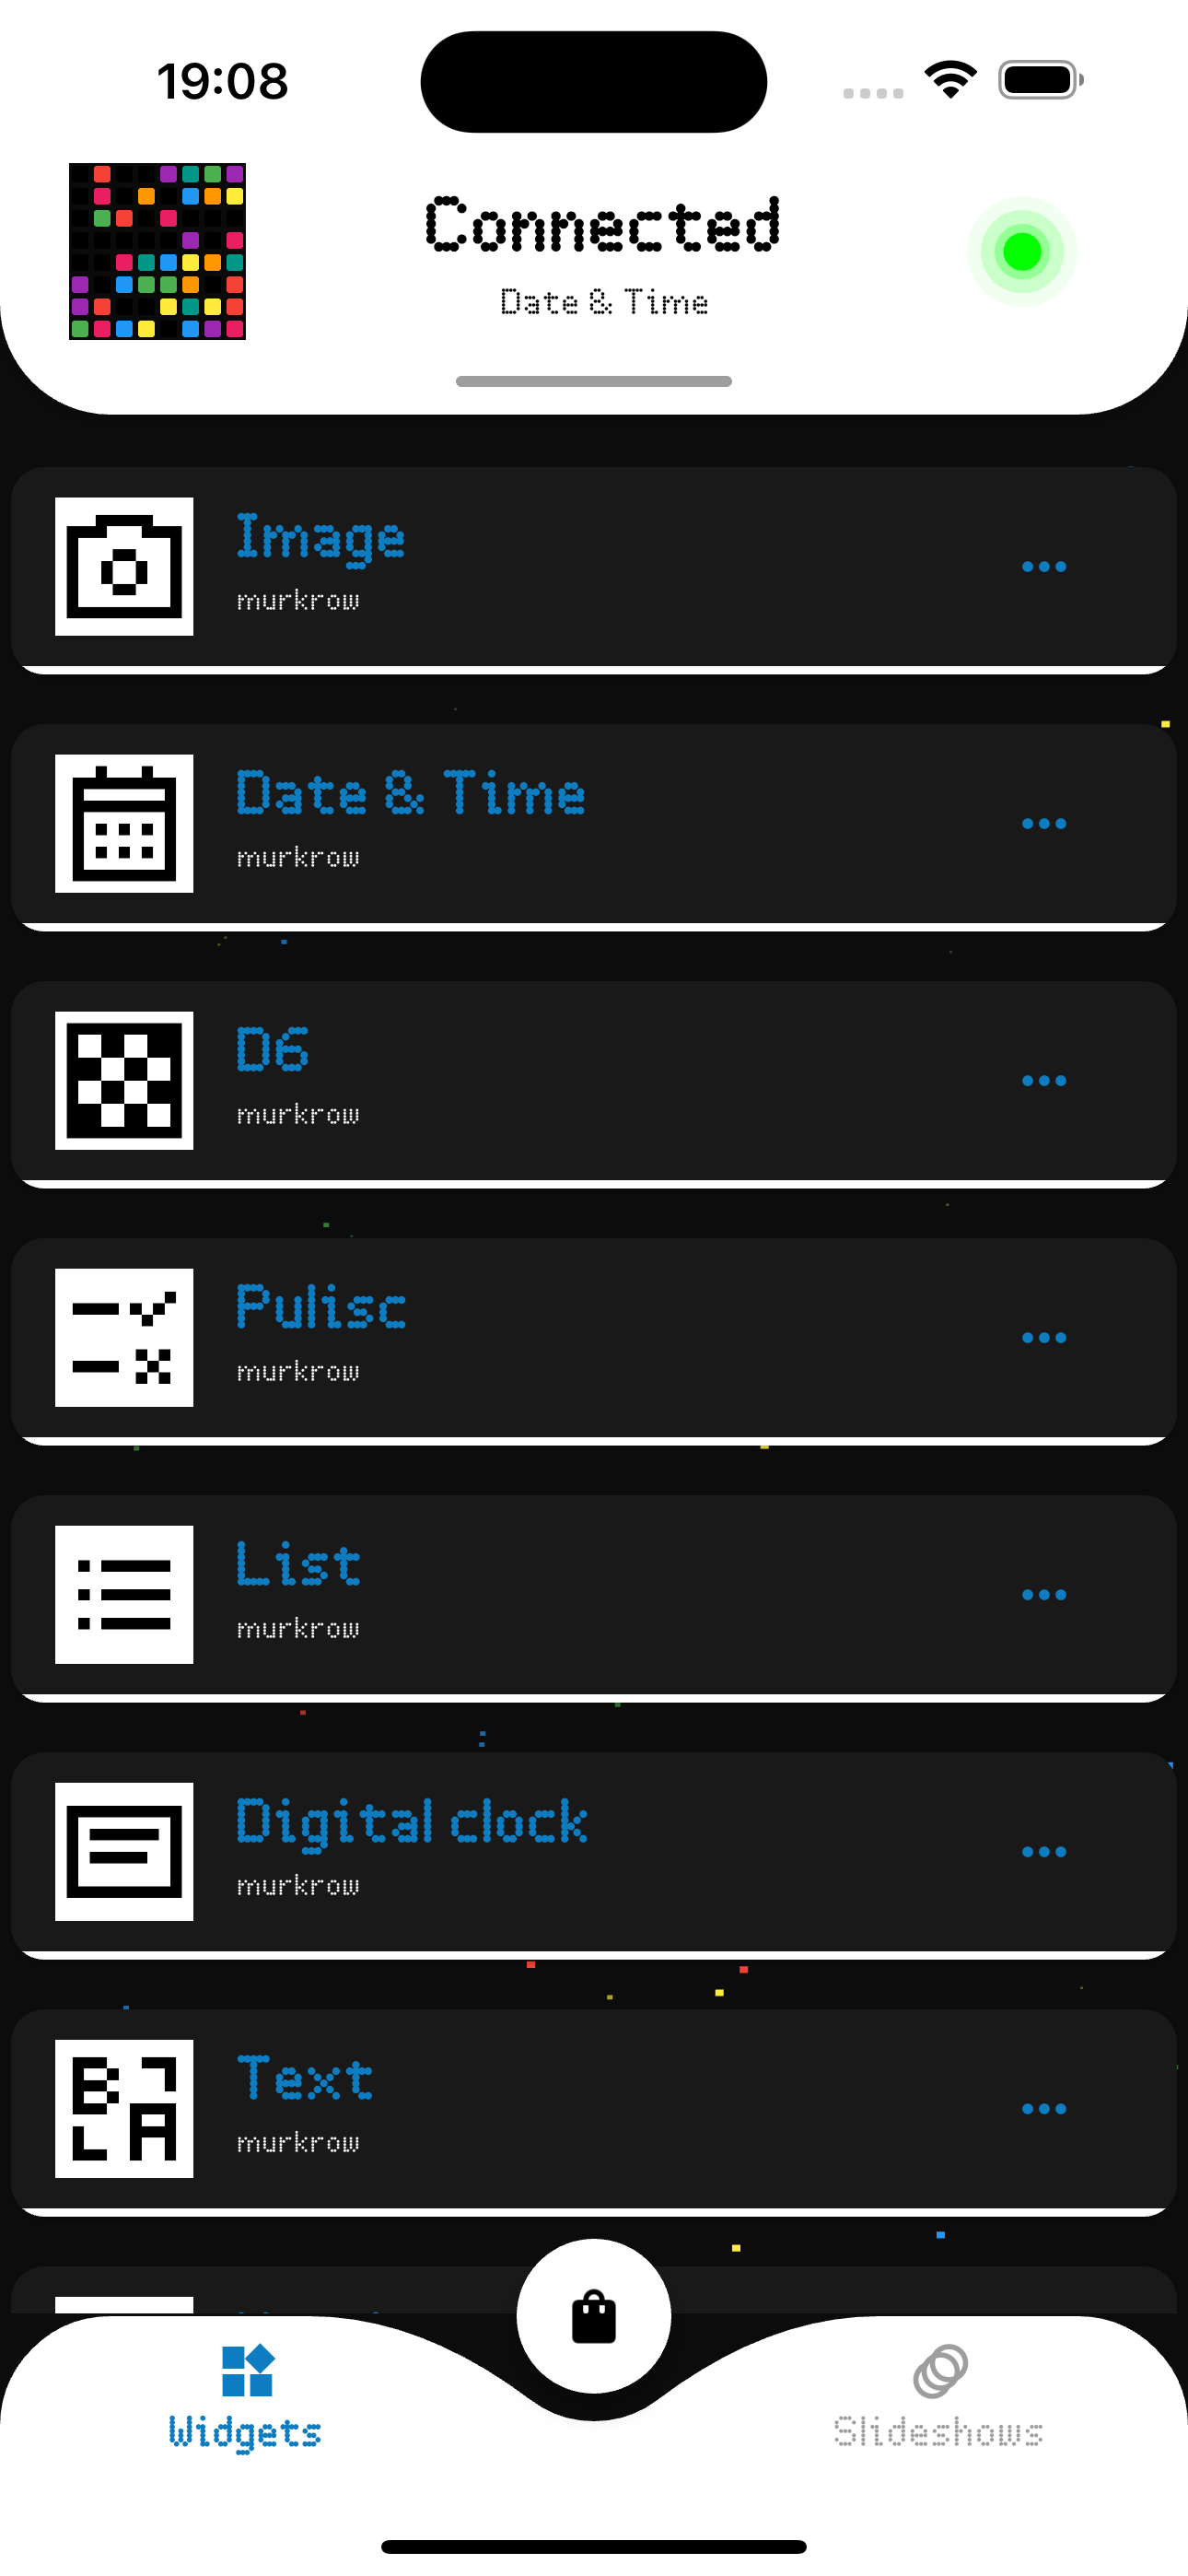
\includegraphics[width=\textwidth]{tesi/img/client_demo/installed_widgets.png}
        \caption*{Installed Widgets}
    \end{minipage}
    \begin{minipage}[b]{0.24\textwidth}
        \centering
        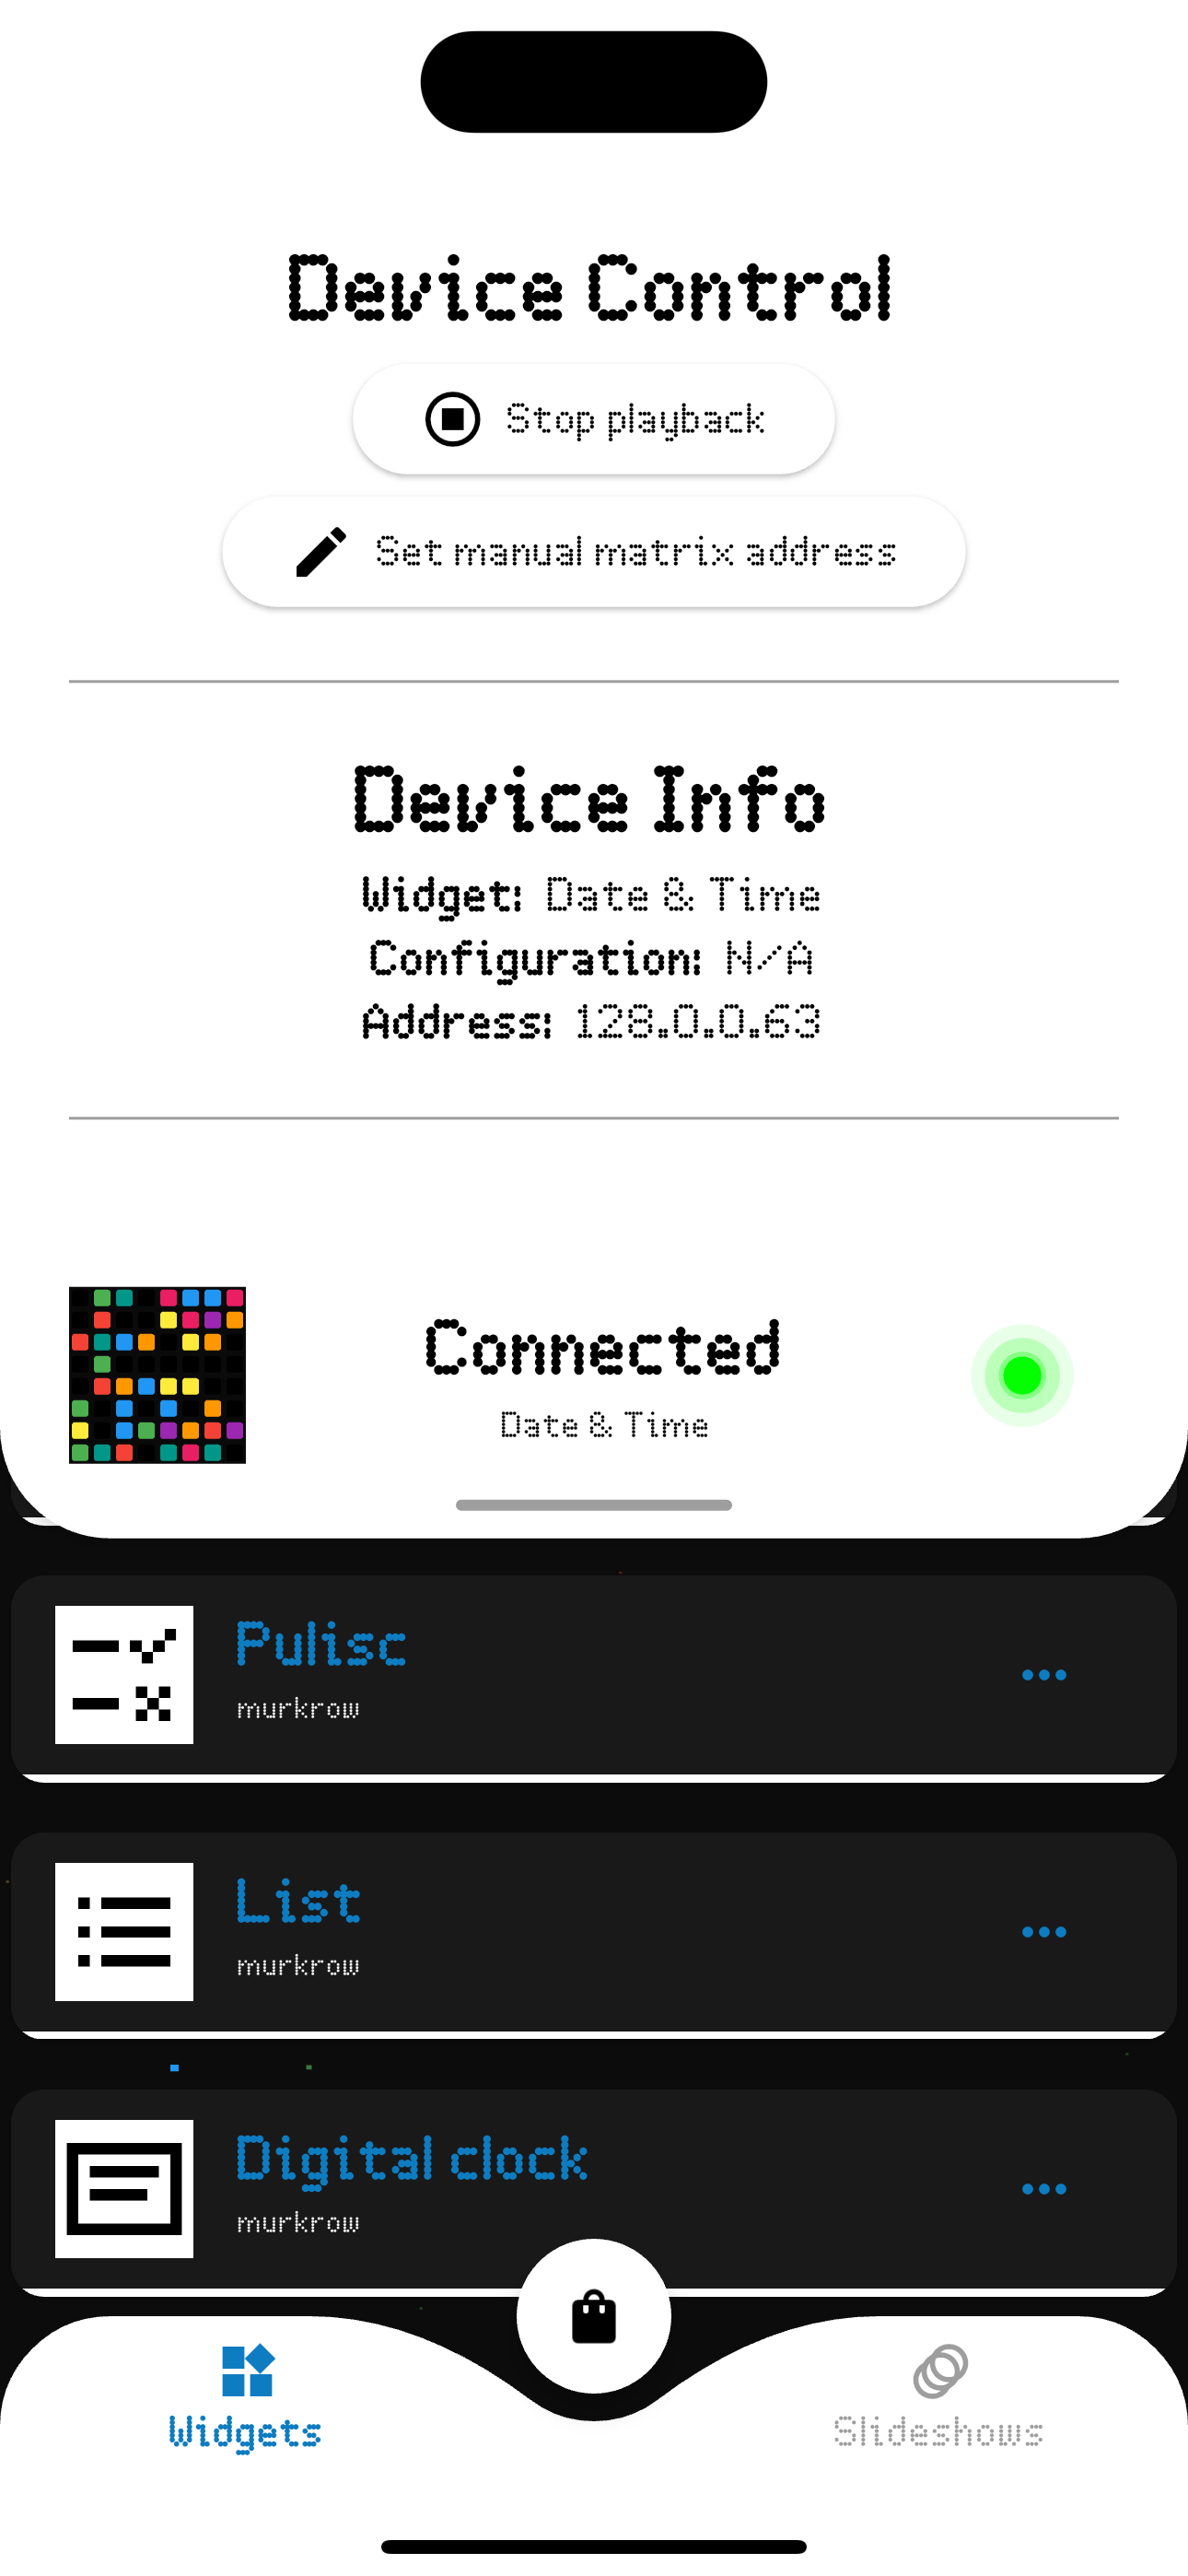
\includegraphics[width=\textwidth]{tesi/img/client_demo/matrix_control.png}
        \caption*{Matrix Control}
    \end{minipage}
    \begin{minipage}[b]{0.24\textwidth}
        \centering
        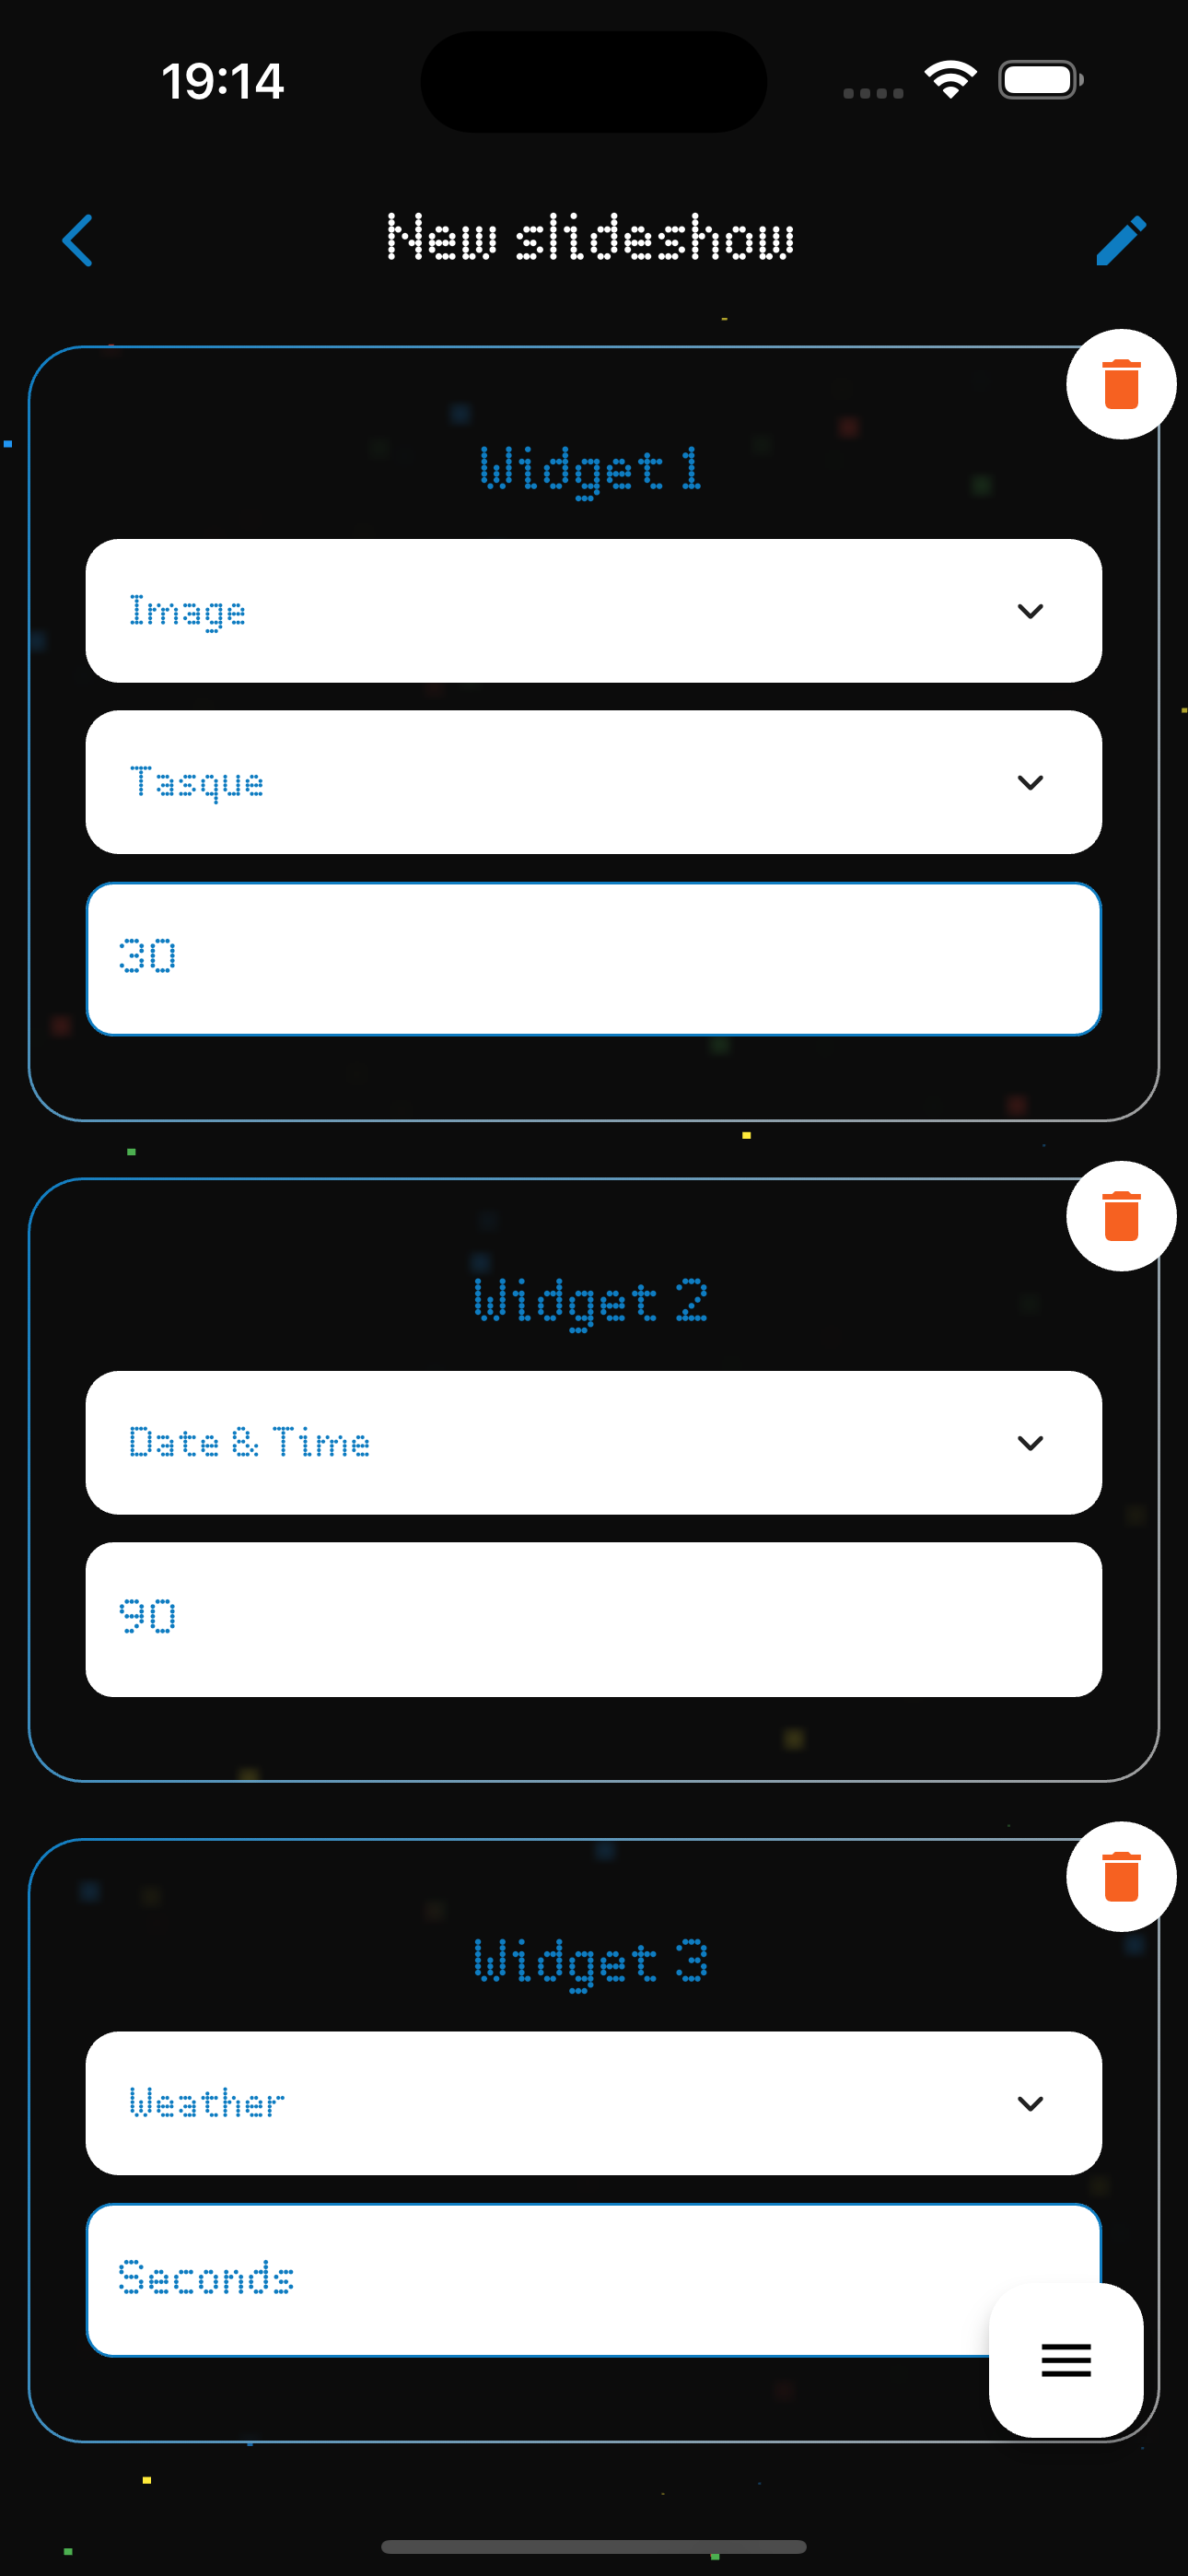
\includegraphics[width=\textwidth]{tesi/img/client_demo/slideshows.png}
        \caption*{Slideshow Editor}
    \end{minipage}
    \begin{minipage}[b]{0.24\textwidth}
        \centering
        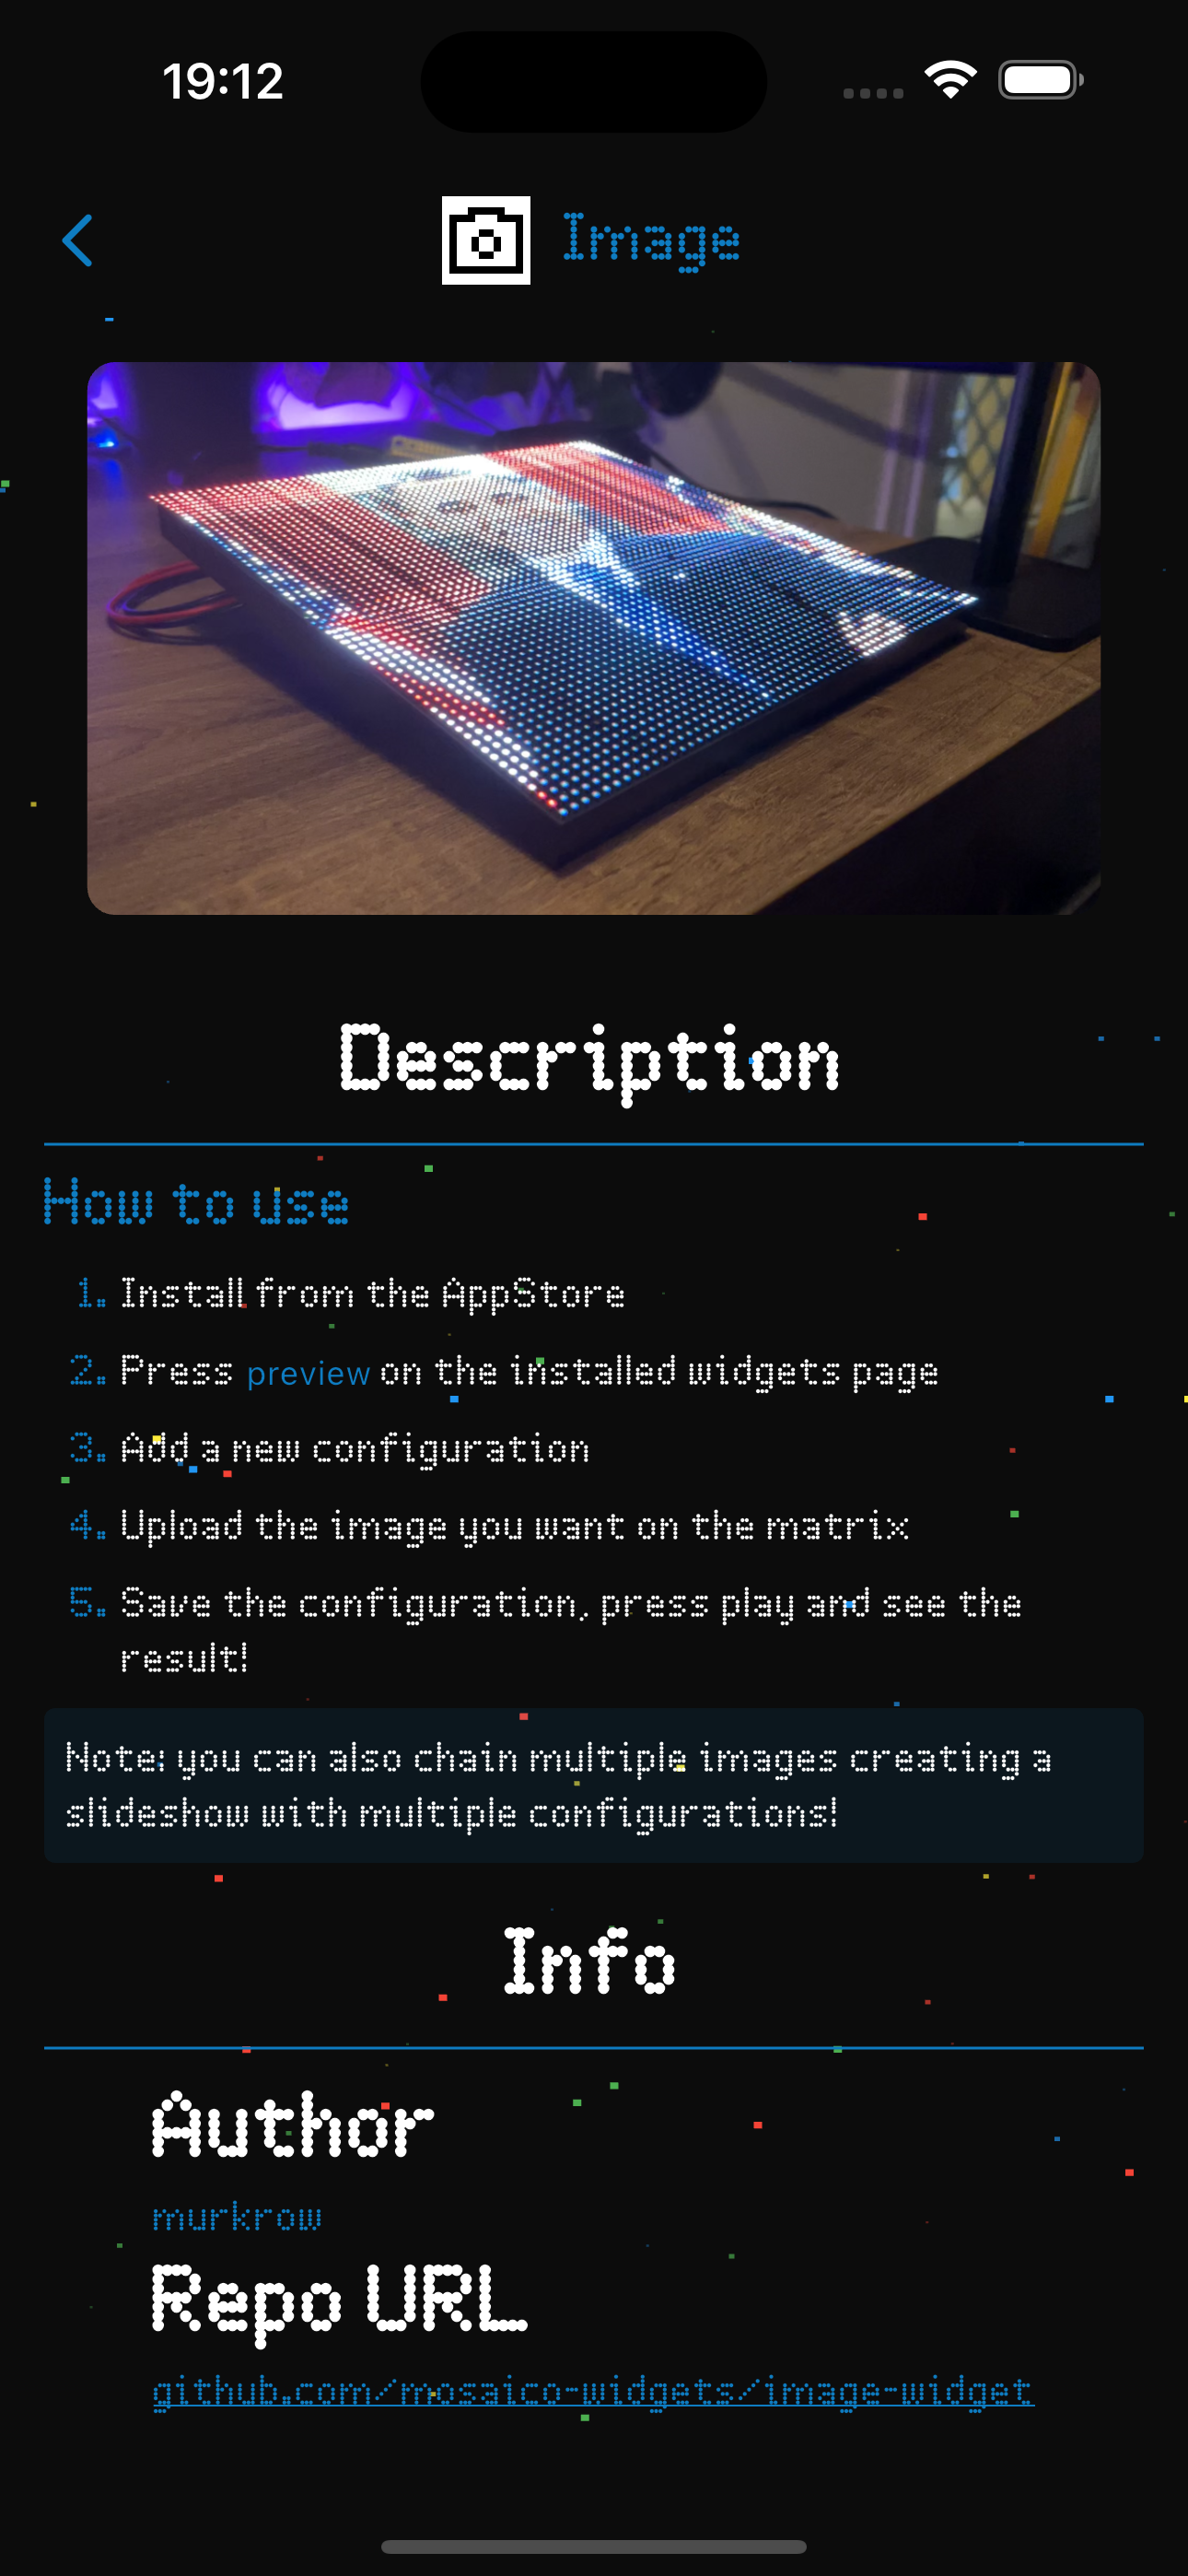
\includegraphics[width=\textwidth]{tesi/img/client_demo/store.png}
        \caption*{Widget Store}
    \end{minipage}
\end{figure}

Creating a companion client for my project was a relatively straightforward task, given my extensive experience as a mobile app developer. However, the distinctive element of this particular app is the use of the Flutter framework. Having worked with both native and web development technologies, I was intrigued by Flutter’s potential, especially since it is a well-regarded, Google-supported framework designed for cross-platform development. Flutter allows developers to create applications for various platforms with minimal additional effort, using a single codebase.

\newpage

\section{Showcase}
\subsection{Home}
Upon launching the application, the user is greeted by a tabbed interface that divides the app into two primary sections: the Installed Widgets page and the Slideshows page. A floating action button located at the center of the bottom navigation bar changes its function depending on the active tab. When viewing the Installed Widgets page, the button displays a shopping bag icon, which opens the widget store when clicked. On the Slideshows page, the button instead shows a "plus" icon, which initiates the creation of a new slideshow.

\begin{figure}[h]
    \centering
    \begin{minipage}[b]{0.45\textwidth}
        \centering
        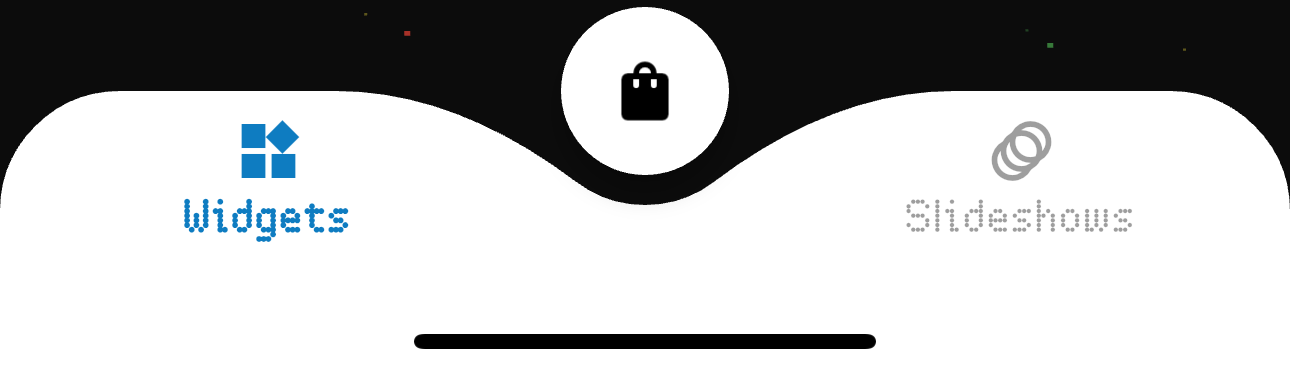
\includegraphics[width=\textwidth]{tesi/img/tab_bar/tab-bar-widgets.png}
        \caption*{Widgets Tab}
    \end{minipage}
    \begin{minipage}[b]{0.45\textwidth}
        \centering
        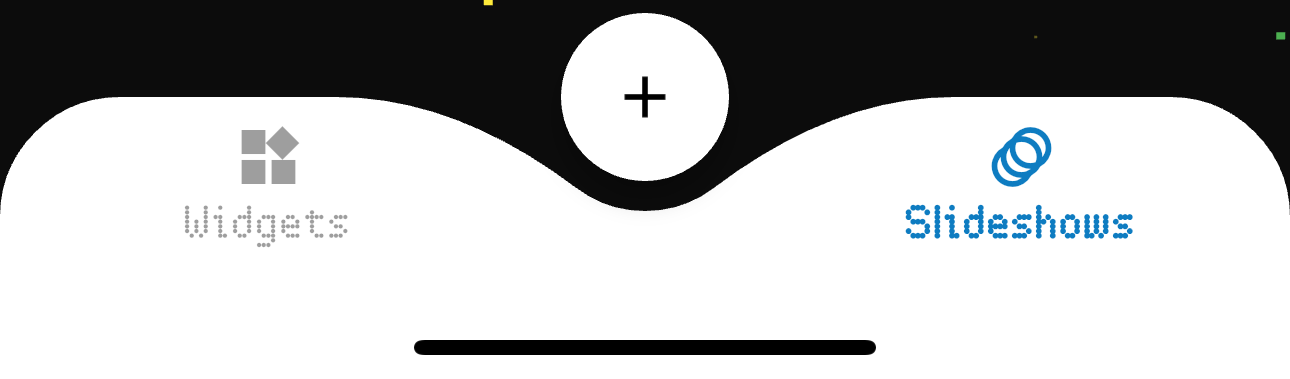
\includegraphics[width=\textwidth]{tesi/img/tab_bar/tab-bar-slideshows.png}
        \caption*{Slideshows Tab}
    \end{minipage}
\end{figure}

\subsection{Matrix Control}
At the top of the screen, a sliding panel displays essential information such as the connection status and the currently active widget. Pulling the panel down reveals further details about the matrix connection, including additional configuration options. Users can perform actions such as stopping playback or manually inputting the matrix's address.

\begin{figure}[h]
    \centering
    \begin{minipage}[b]{0.32\textwidth}
        \centering
        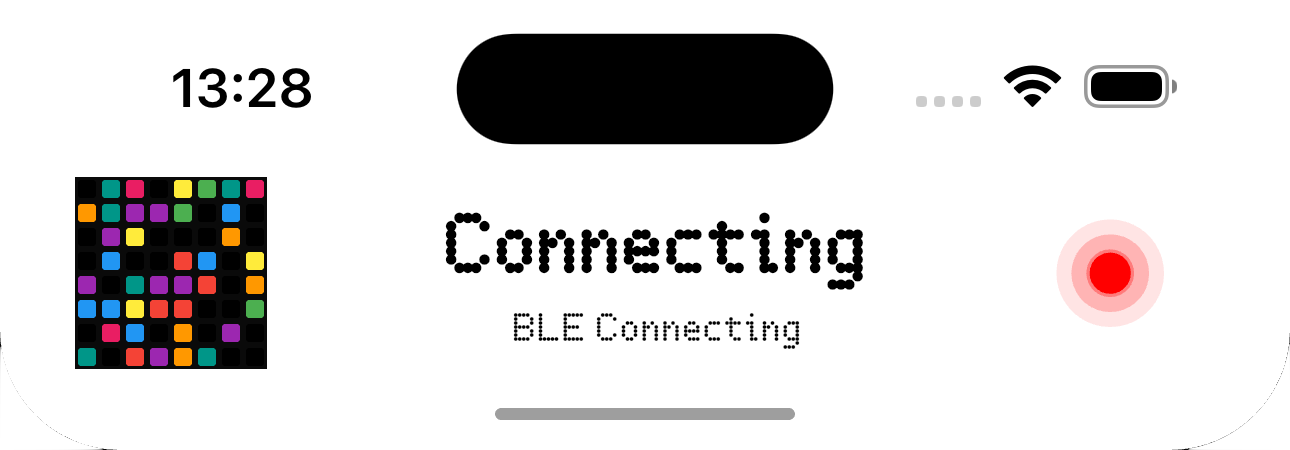
\includegraphics[width=\textwidth]{tesi/img/matrix_status_notch/connecting.png}
        \caption*{Connecting to Matrix}
    \end{minipage}
    \begin{minipage}[b]{0.32\textwidth}
        \centering
        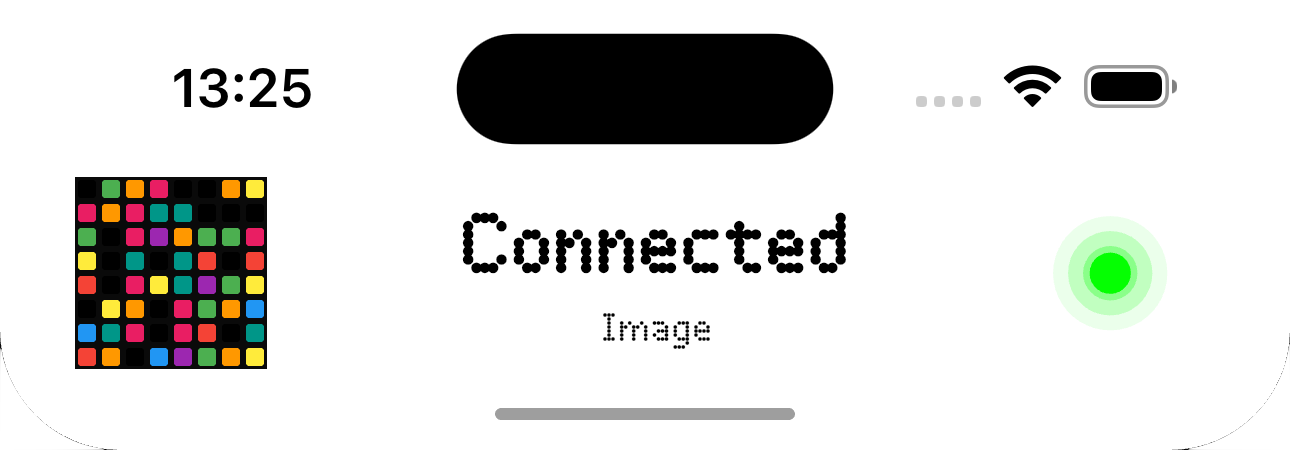
\includegraphics[width=\textwidth]{tesi/img/matrix_status_notch/connected.png}
        \caption*{Matrix Connected}
    \end{minipage}
    \begin{minipage}[b]{0.32\textwidth}
        \centering
        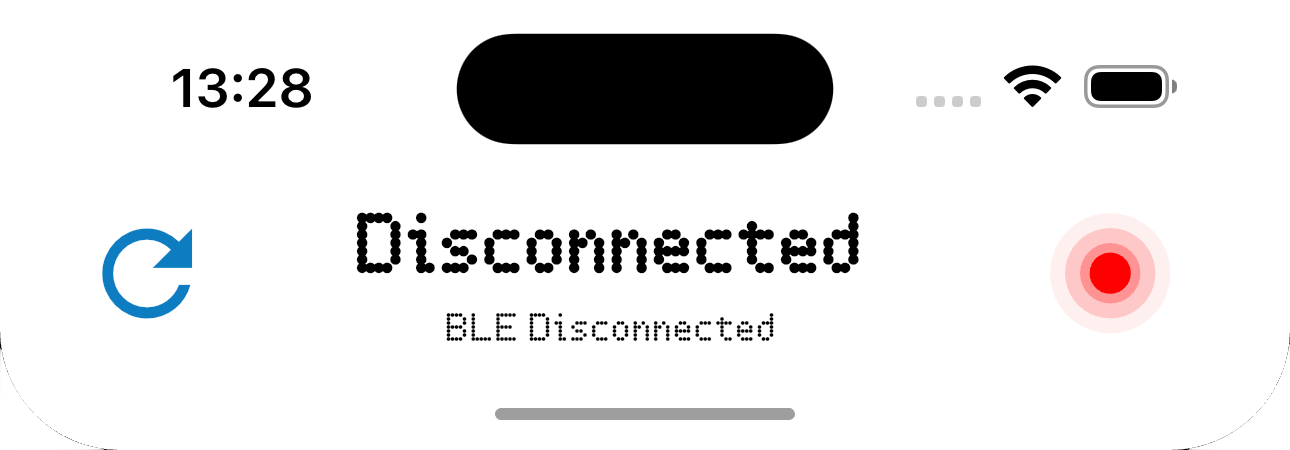
\includegraphics[width=\textwidth]{tesi/img/matrix_status_notch/disconnected.png}
        \caption*{Matrix Not Reachable}
    \end{minipage}
\end{figure}

\newpage

\subsection{Installed Widgets}
This is the default screen presented when the app launches. It lists all the widgets currently installed on the matrix, which have been downloaded from the store. Users can activate a widget by simply tapping on it. If the widget does not require further configuration, it will be displayed immediately on the matrix. However, if it is configurable, a configuration selector will prompt the user to choose a specific configuration before activating the widget.

\begin{figure}[h]
    \centering
    \begin{minipage}[b]{0.32\textwidth}
        \centering
        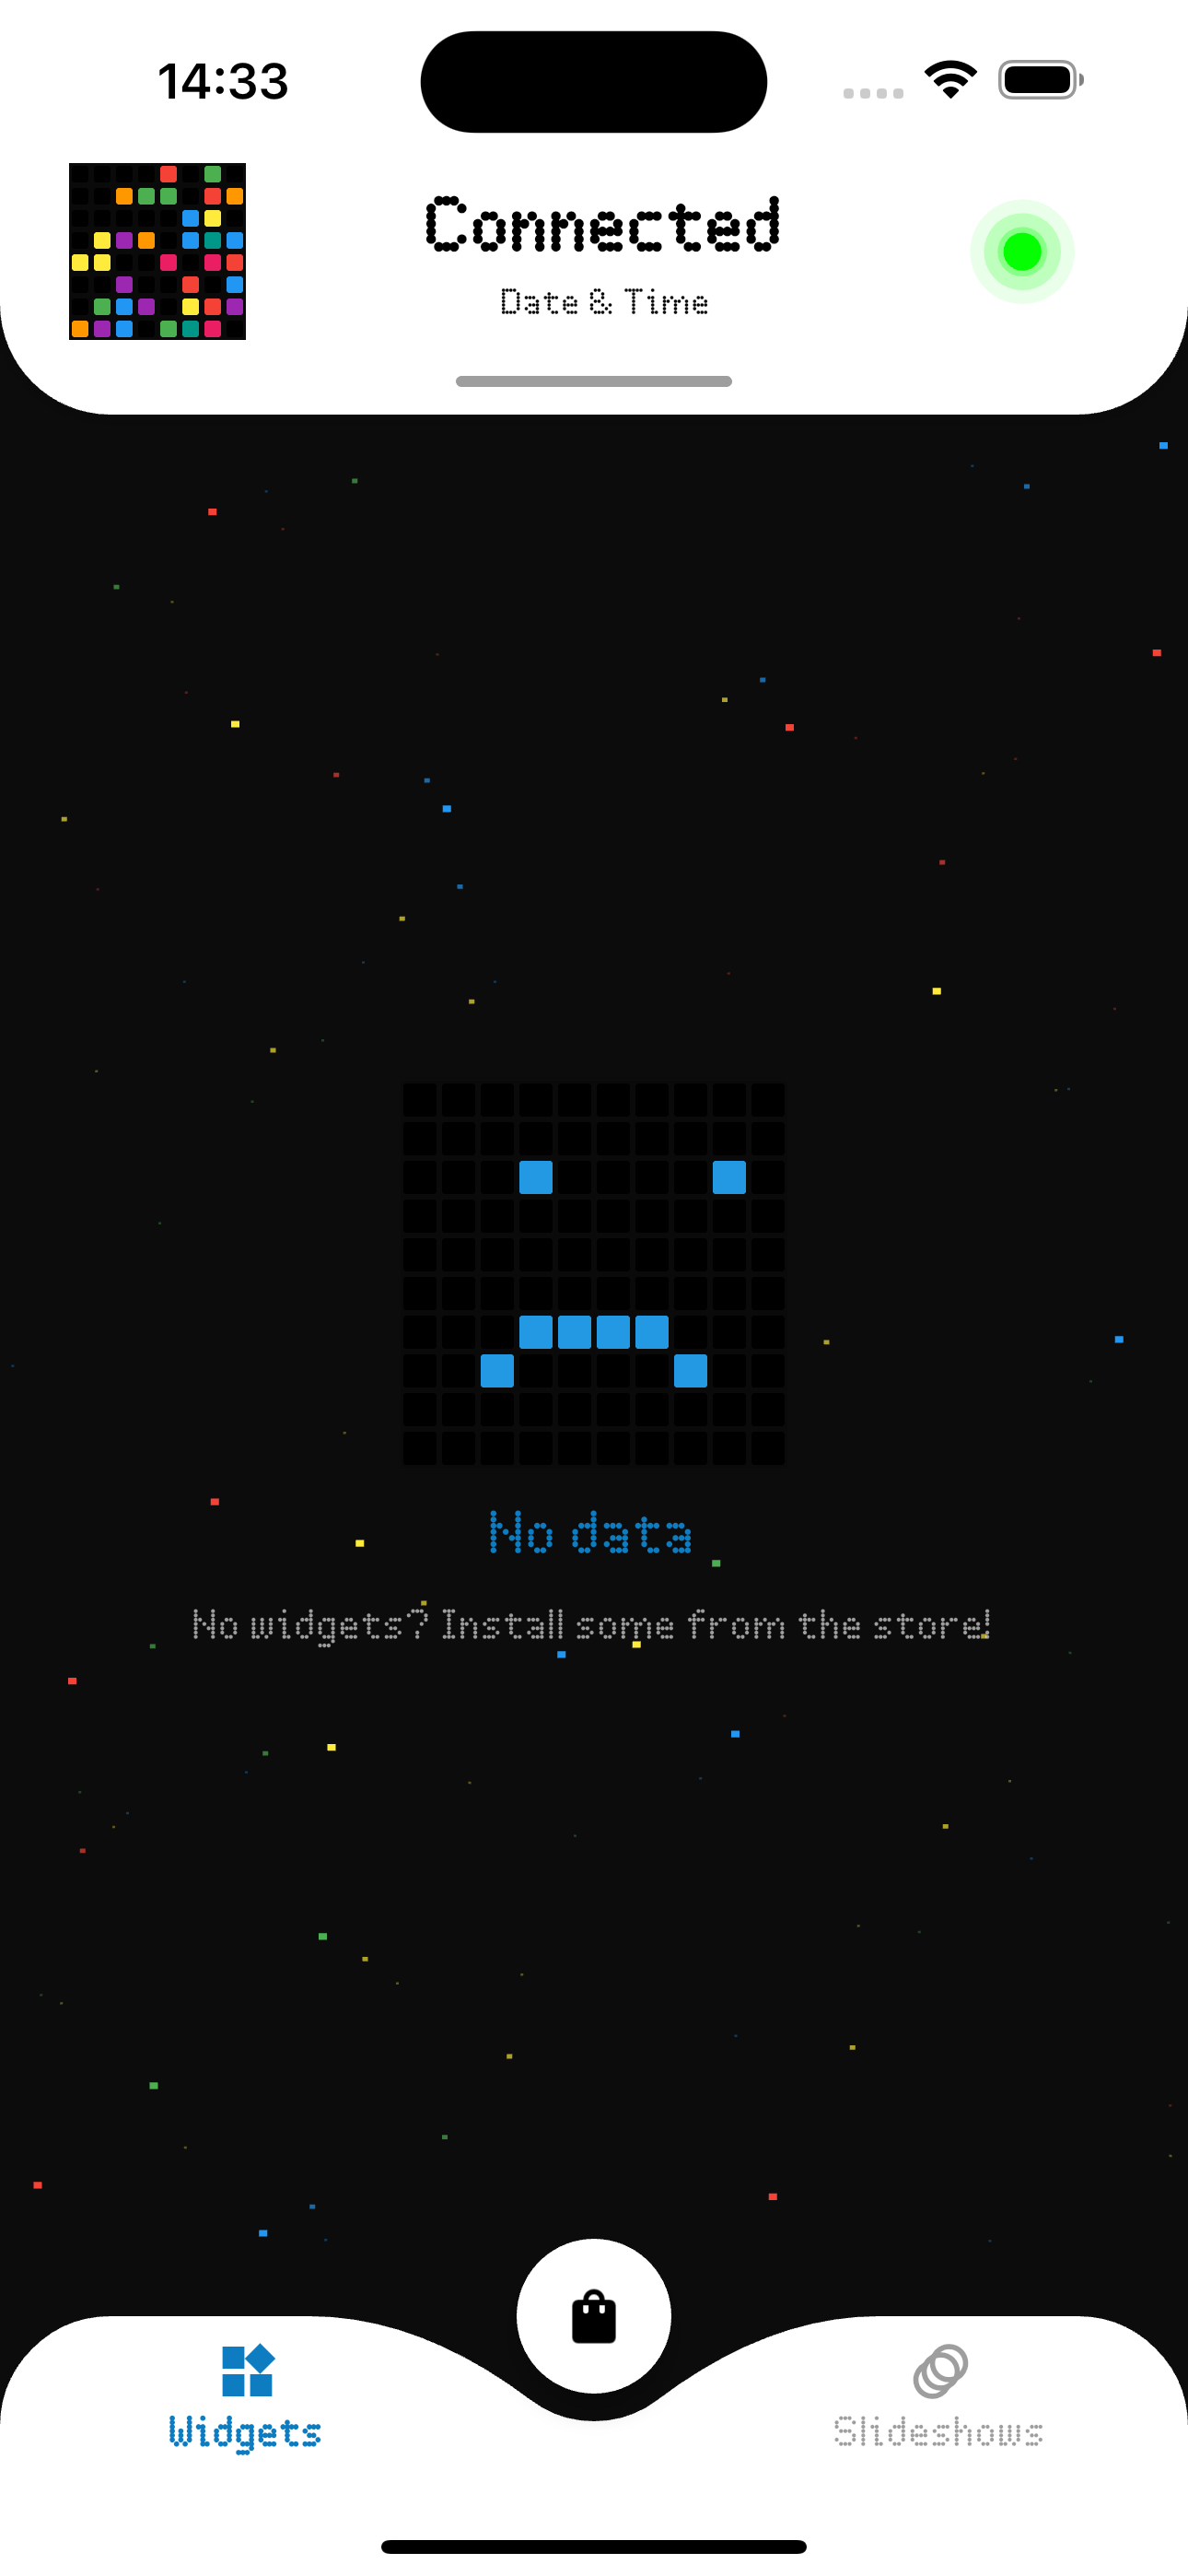
\includegraphics[width=\textwidth]{tesi/img/client_demo/installed_widgets/no_data.png}
        \caption*{No Widgets Installed}
    \end{minipage}
    \begin{minipage}[b]{0.32\textwidth}
        \centering
        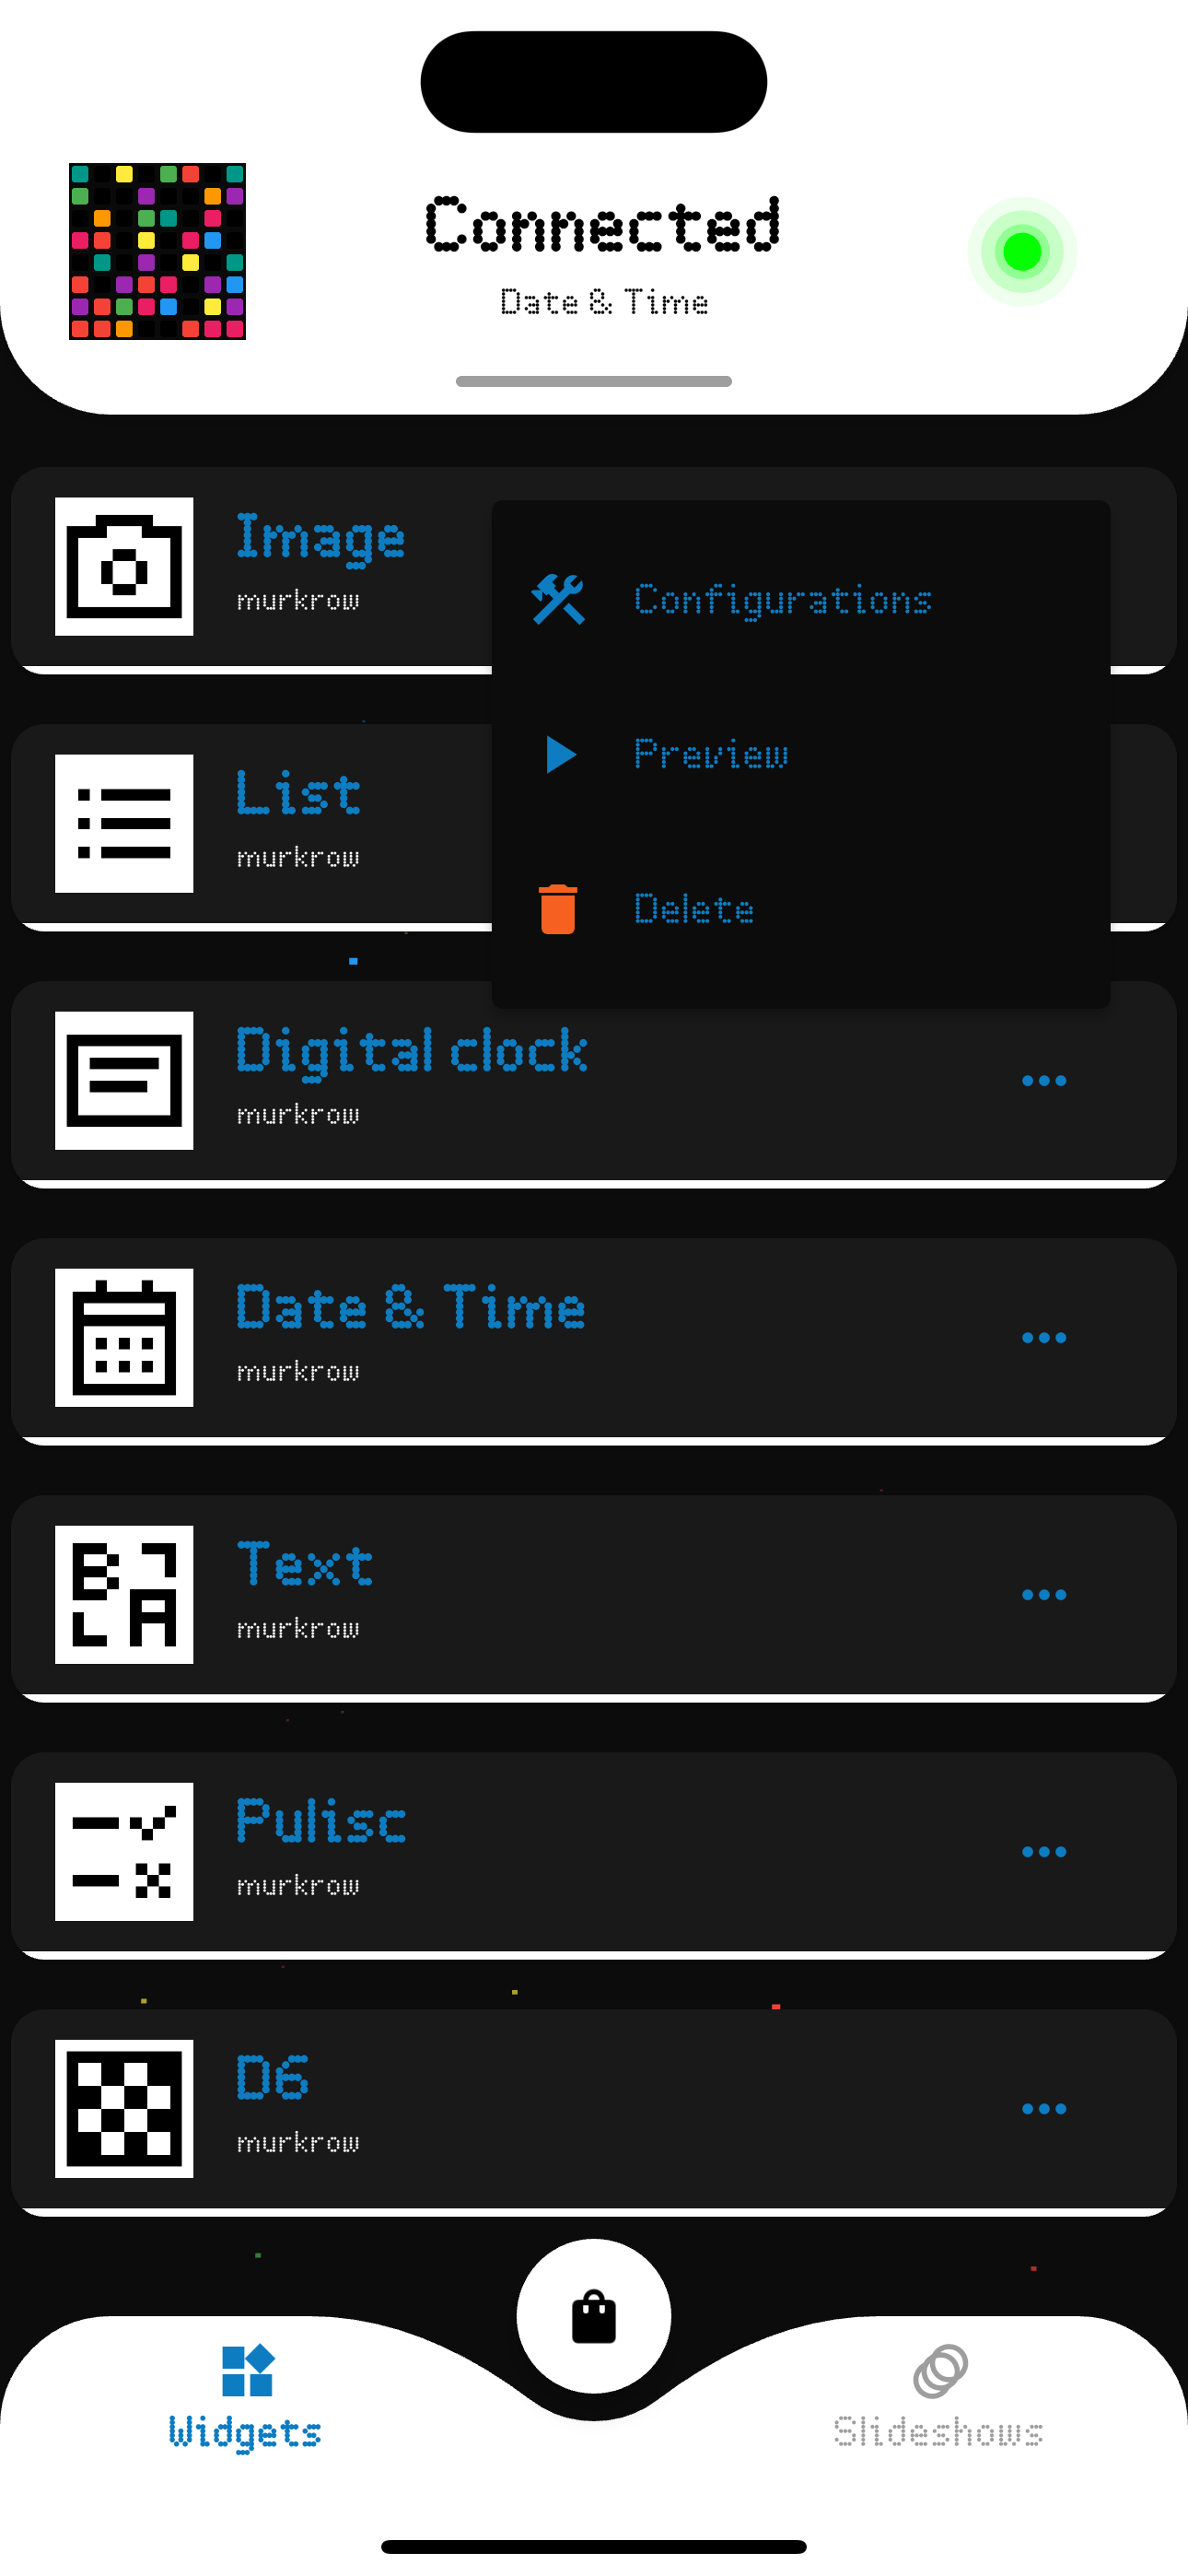
\includegraphics[width=\textwidth]{tesi/img/client_demo/installed_widgets/page.png}
        \caption*{Installed Widget Actions}
    \end{minipage}
    \begin{minipage}[b]{0.32\textwidth}
        \centering
        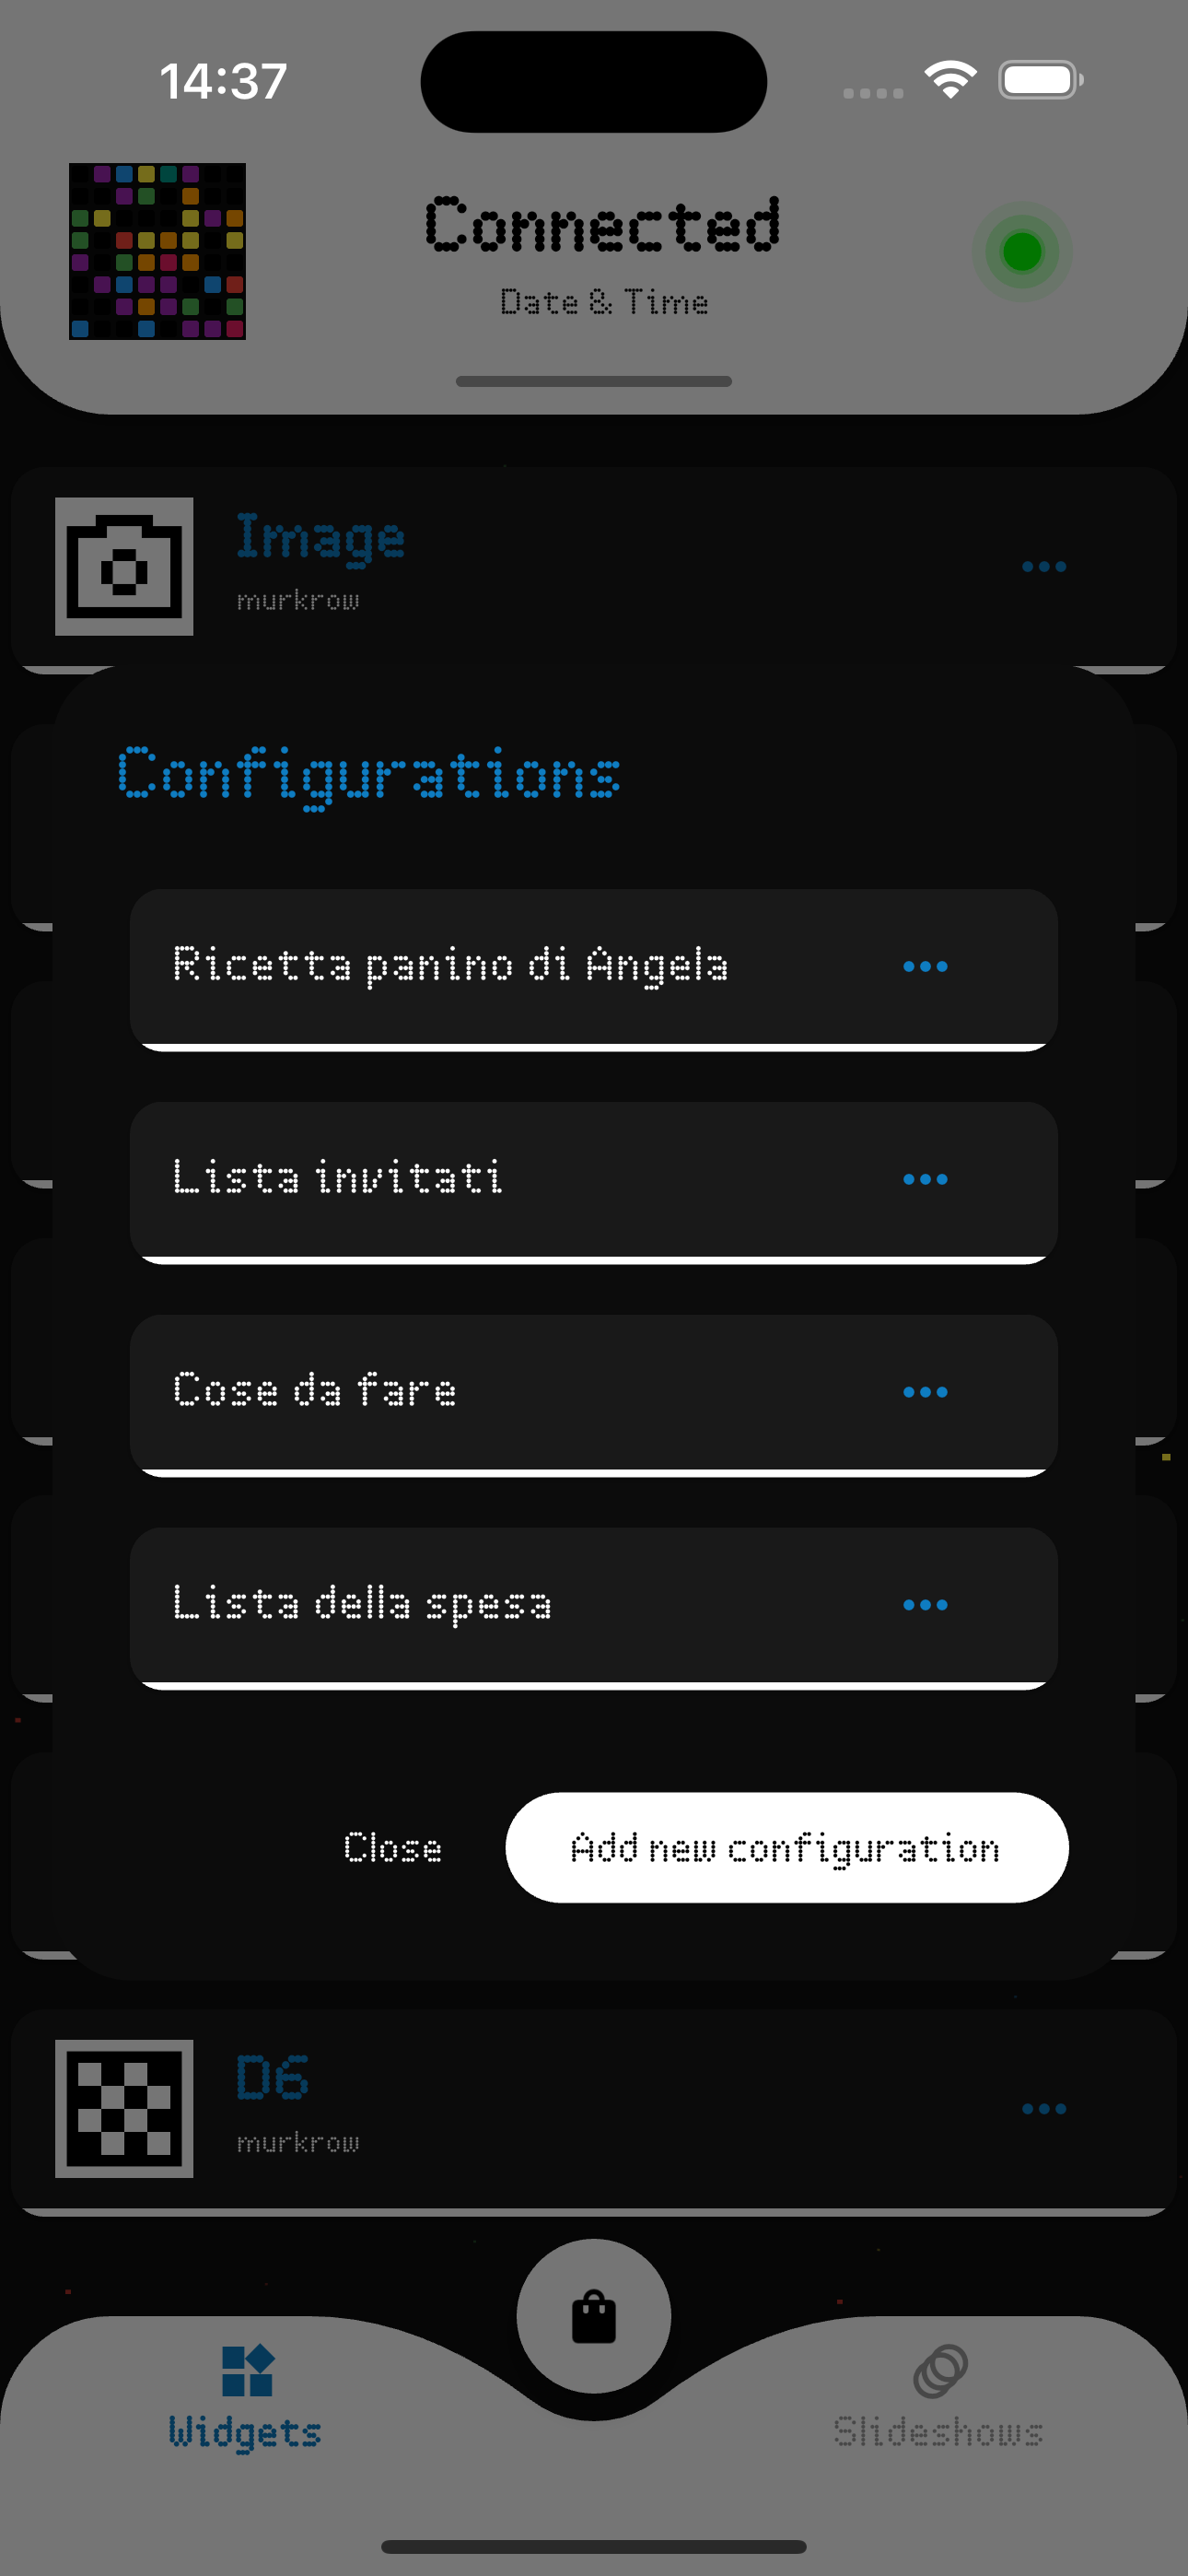
\includegraphics[width=\textwidth]{tesi/img/client_demo/installed_widgets/config_choice.png}
        \caption*{Configuration Selector}
    \end{minipage}
\end{figure}
\newpage
\subsection{Widget Store}
The widget store provides users with a space to discover new widgets. A main page lists all available widgets, each represented by a tile. By clicking on a tile, users can view more detailed information about the widget, including an image carousel, a rich markdown description, and details about the widget’s author and source code. Notably, all widgets in the store must be uploaded to a publicly accessible repository, ensuring that the ecosystem remains entirely open-source.

\begin{figure}[h]
    \centering
    \begin{minipage}[b]{0.32\textwidth}
        \centering
        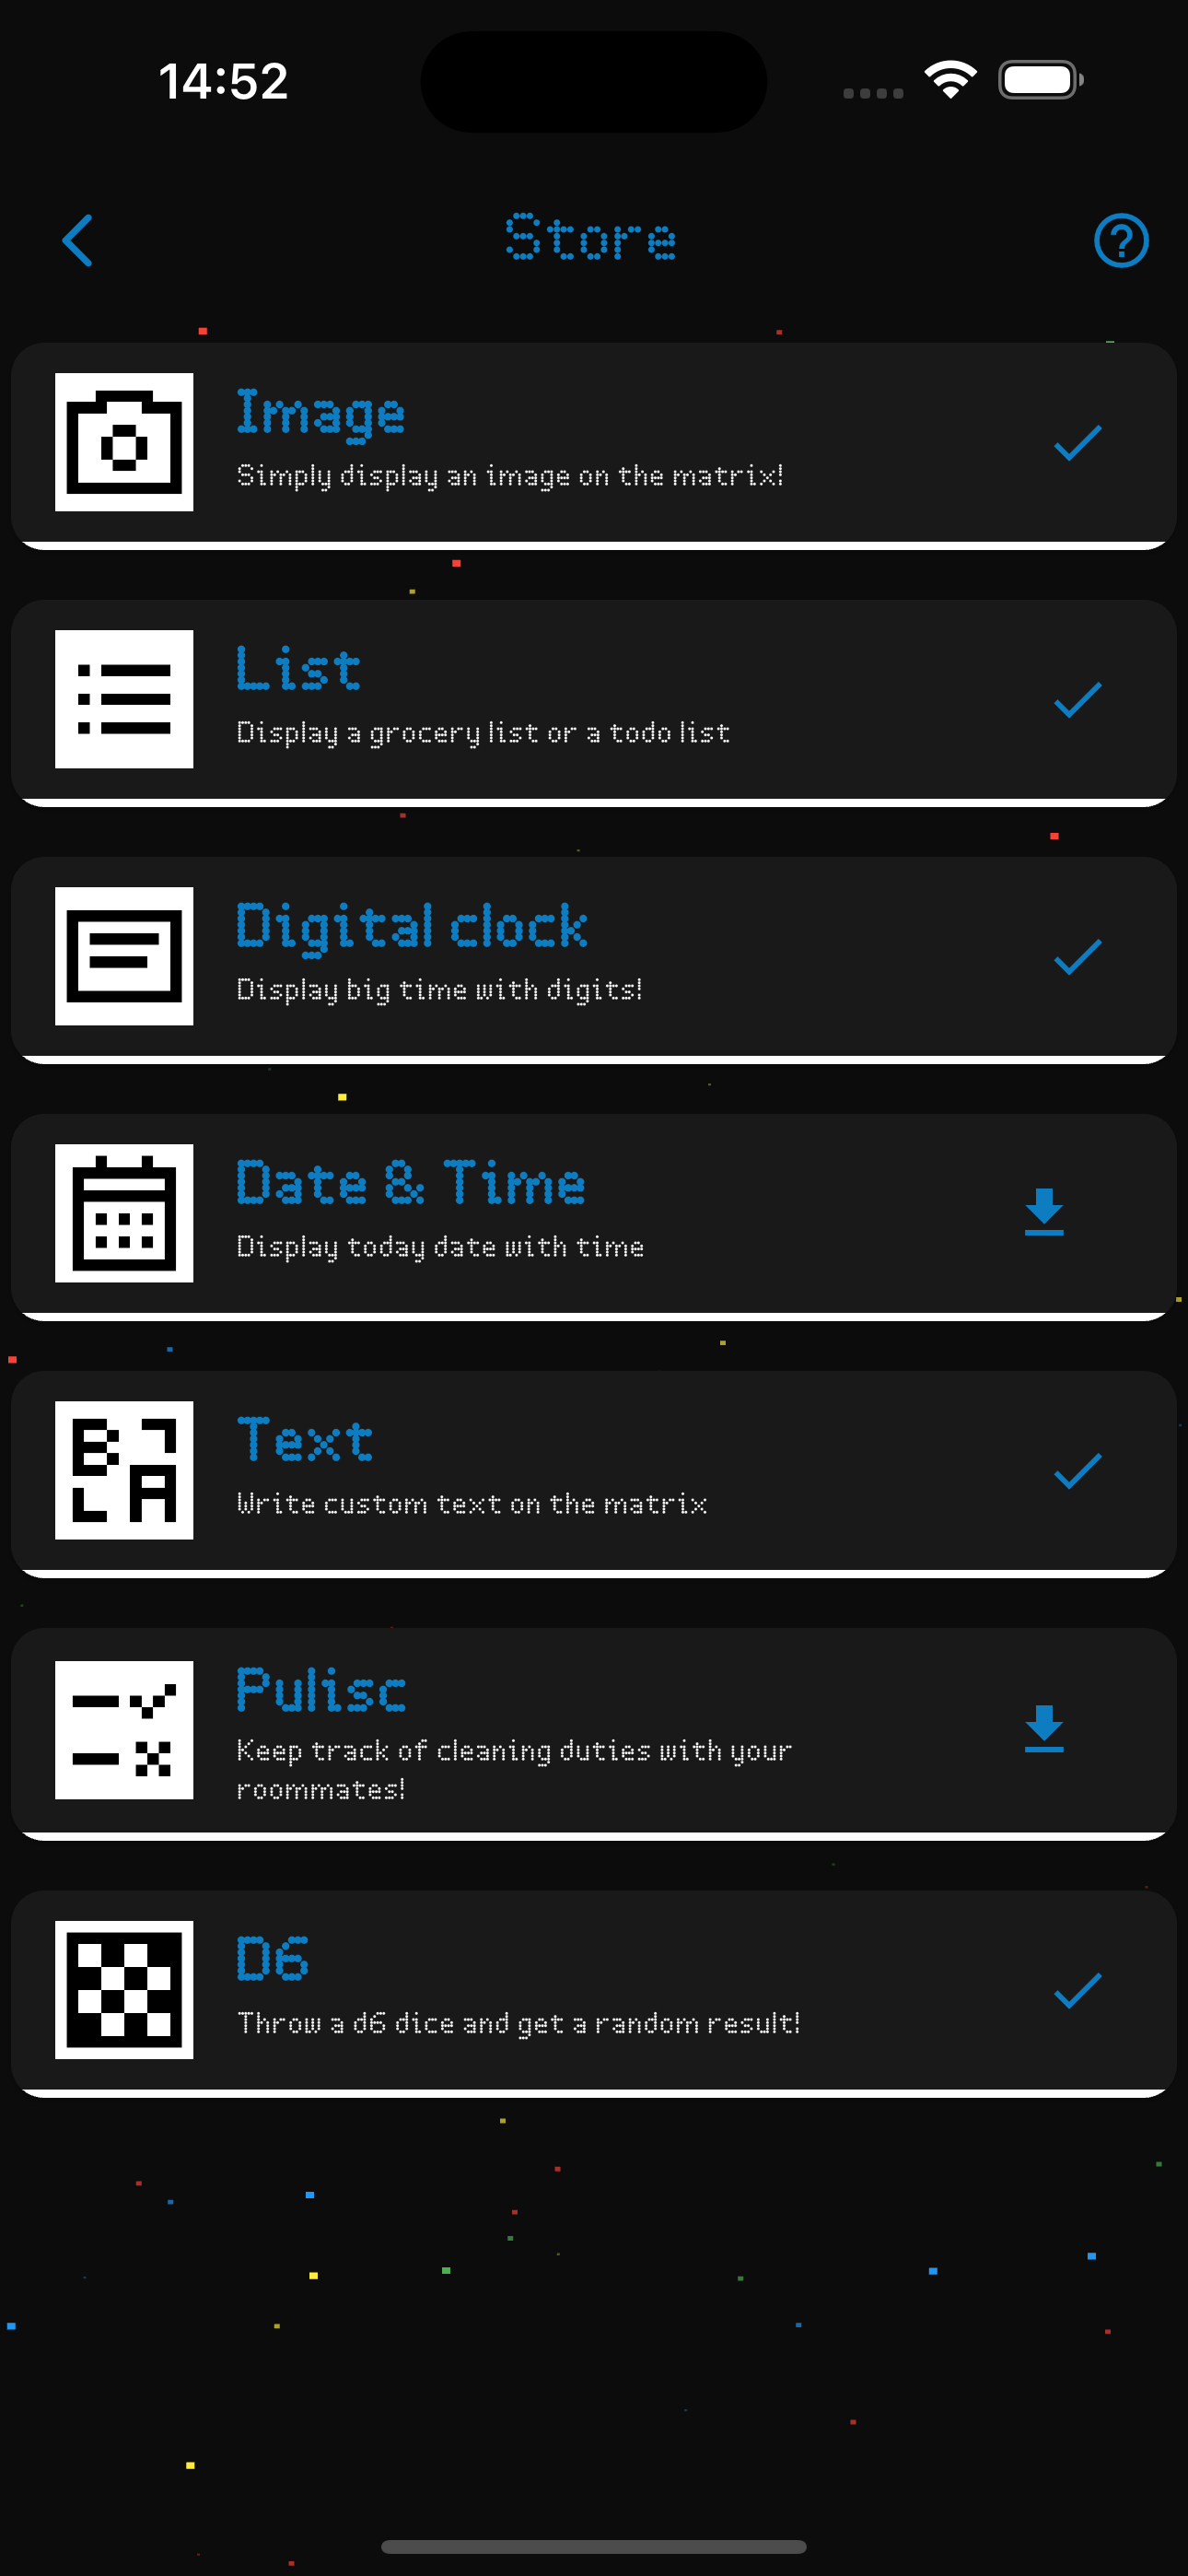
\includegraphics[width=\textwidth]{tesi/img/client_demo/store/page.png}
        \caption*{Store Overview}
    \end{minipage}
    \begin{minipage}[b]{0.32\textwidth}
        \centering
        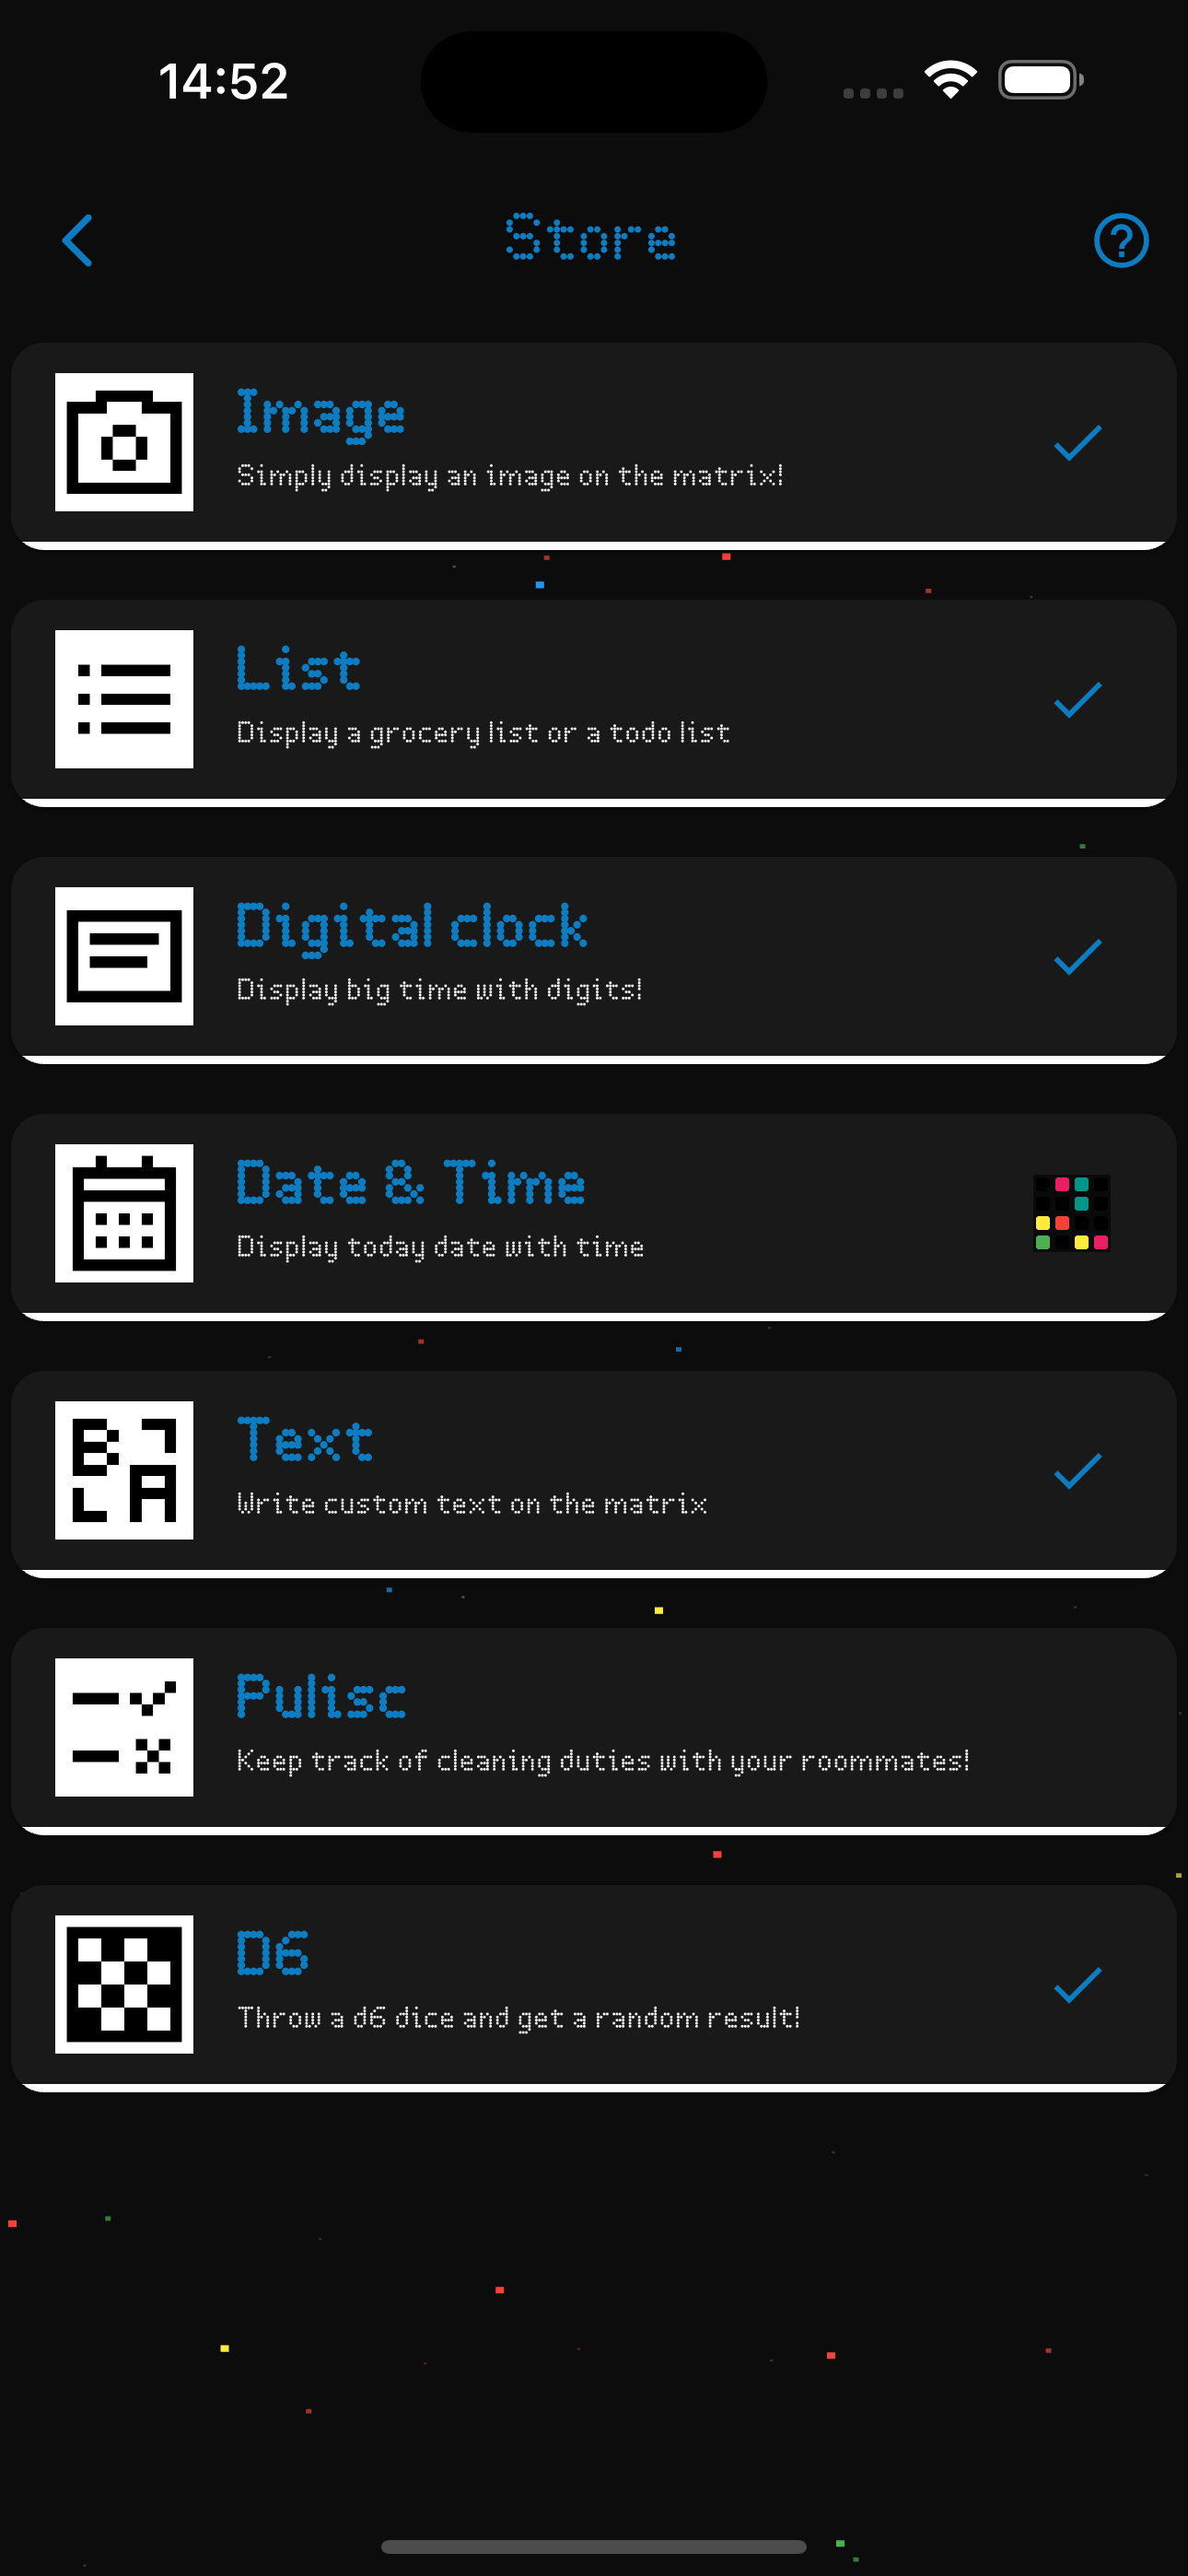
\includegraphics[width=\textwidth]{tesi/img/client_demo/store/widget_installing.png}
        \caption*{Installing a Widget}
    \end{minipage}
    \begin{minipage}[b]{0.32\textwidth}
        \centering
        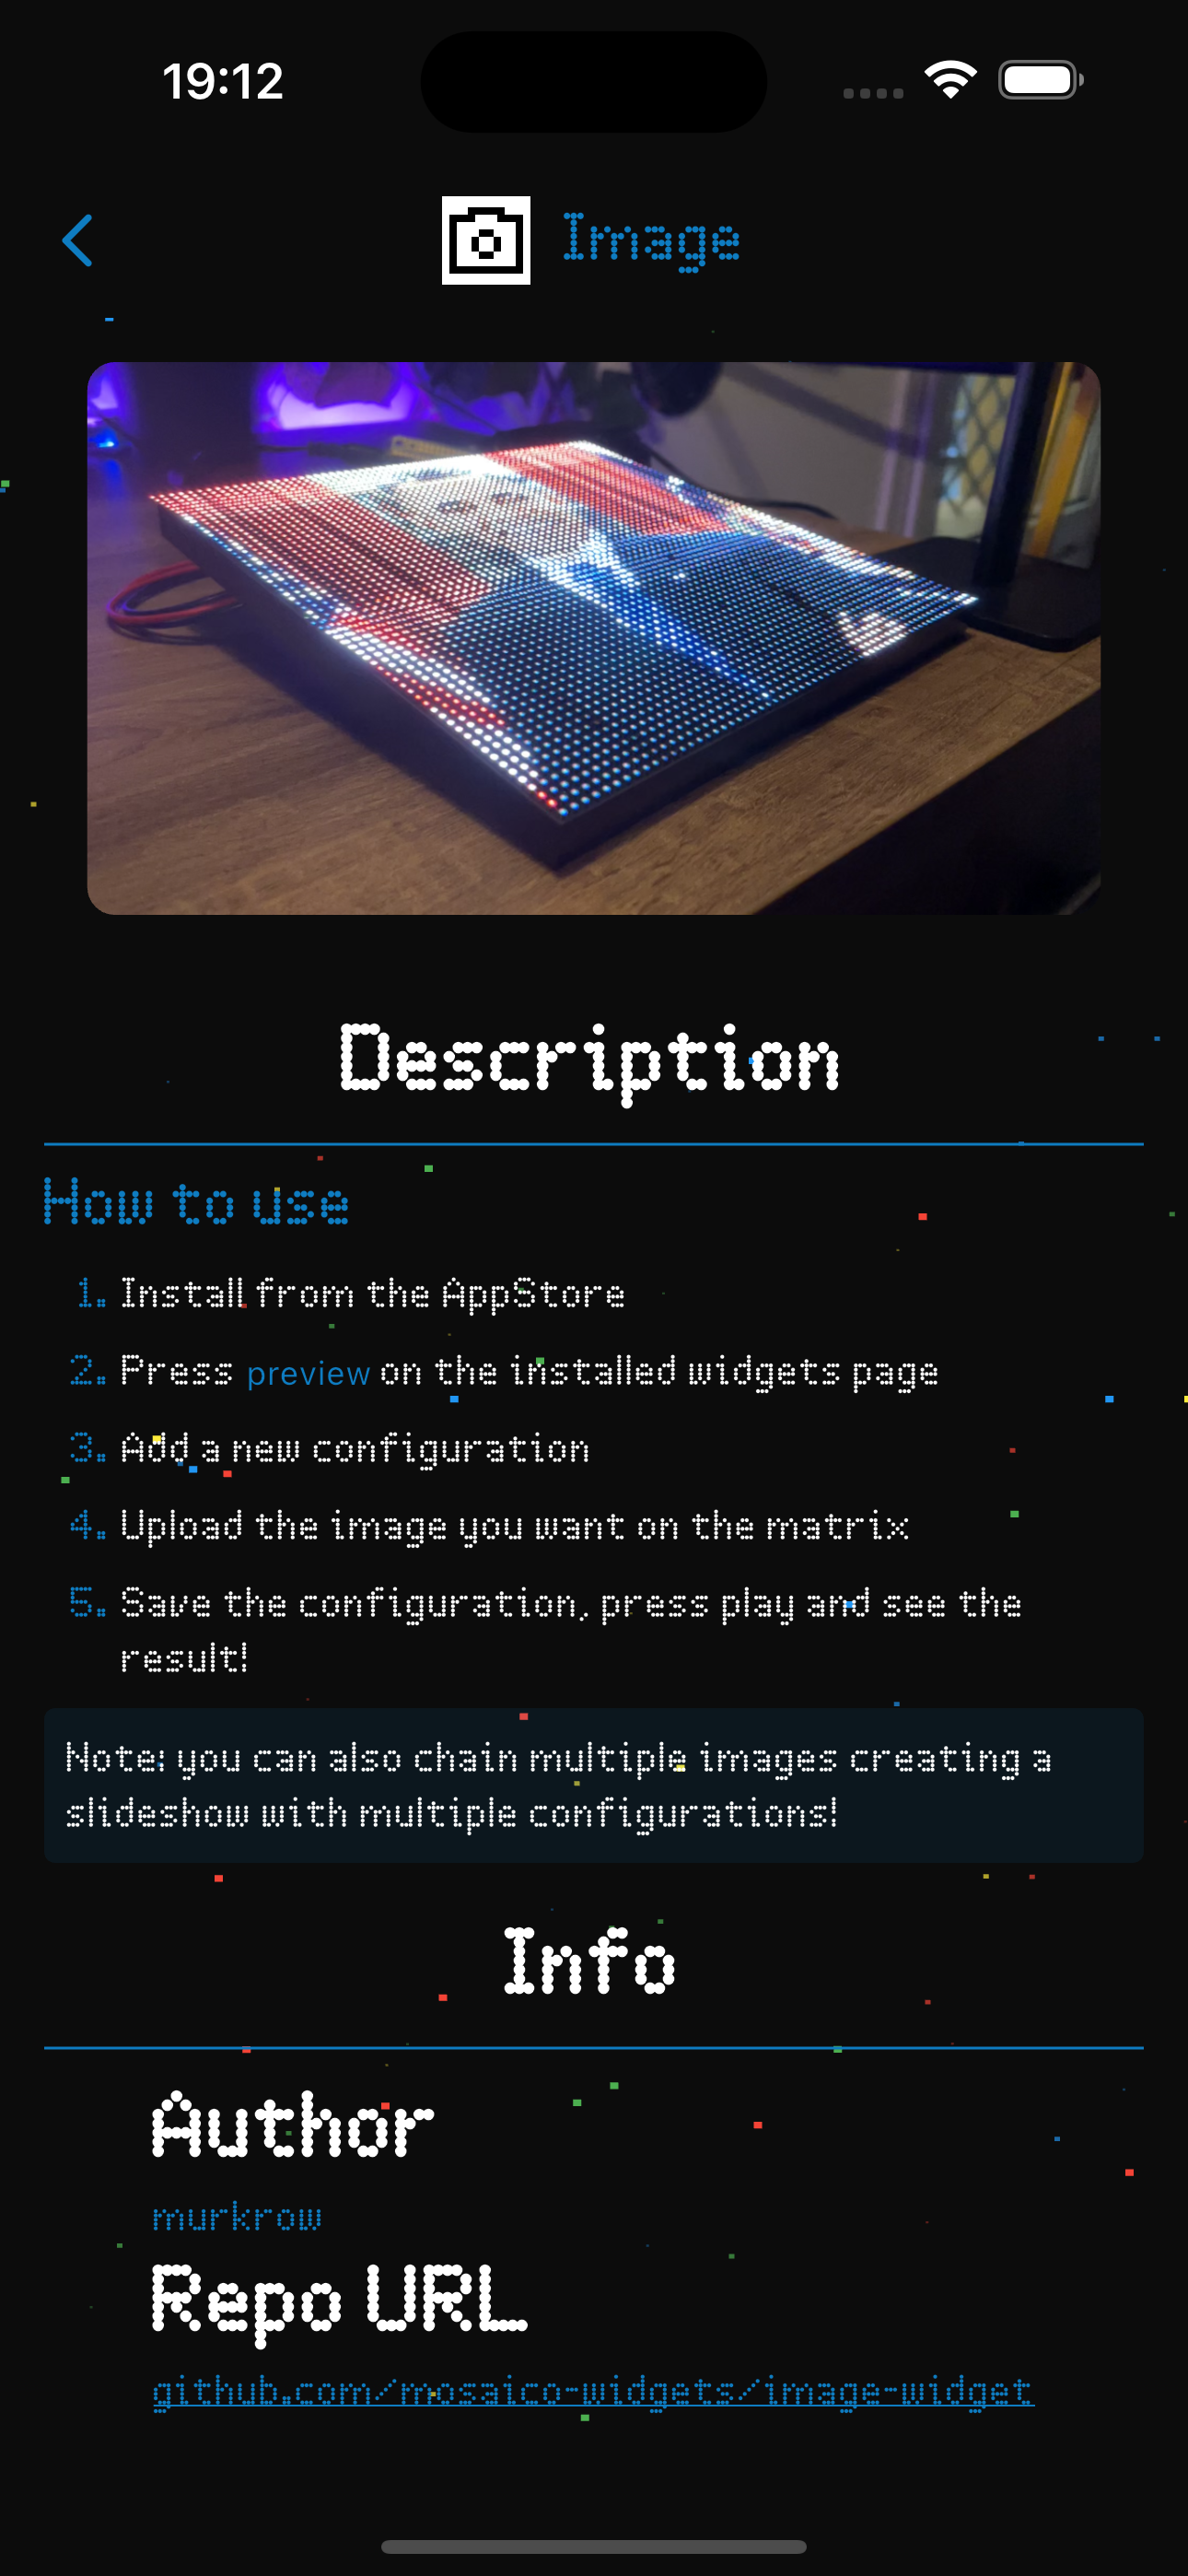
\includegraphics[width=\textwidth]{tesi/img/client_demo/store.png}
        \caption*{Widget Details}
    \end{minipage}
\end{figure}

\subsection{Slideshows}
Slideshows are sequences of widgets displayed consecutively on the matrix. This feature is particularly useful when users prefer to cycle through multiple widgets rather than display a single one continuously.

Creating a new slideshow is intuitive. Users are presented with cards containing two fields: a widget selector and a duration field where they can input the display time in seconds. If the selected widget is configurable, a third field will appear, allowing users to select a specific configuration for that item.

A floating action button in the bottom-right corner expands to provide three actions:
\begin{itemize}
    \item \textbf{Plus Icon}: Adds a new slideshow item card.
    \item \textbf{Save Icon}: Saves the current slideshow or creates a new one.
    \item \textbf{Play Icon}: Saves and immediately plays the current slideshow on the matrix.
\end{itemize}

\begin{figure}[h]
    \centering
    \begin{minipage}[b]{0.32\textwidth}
        \centering
        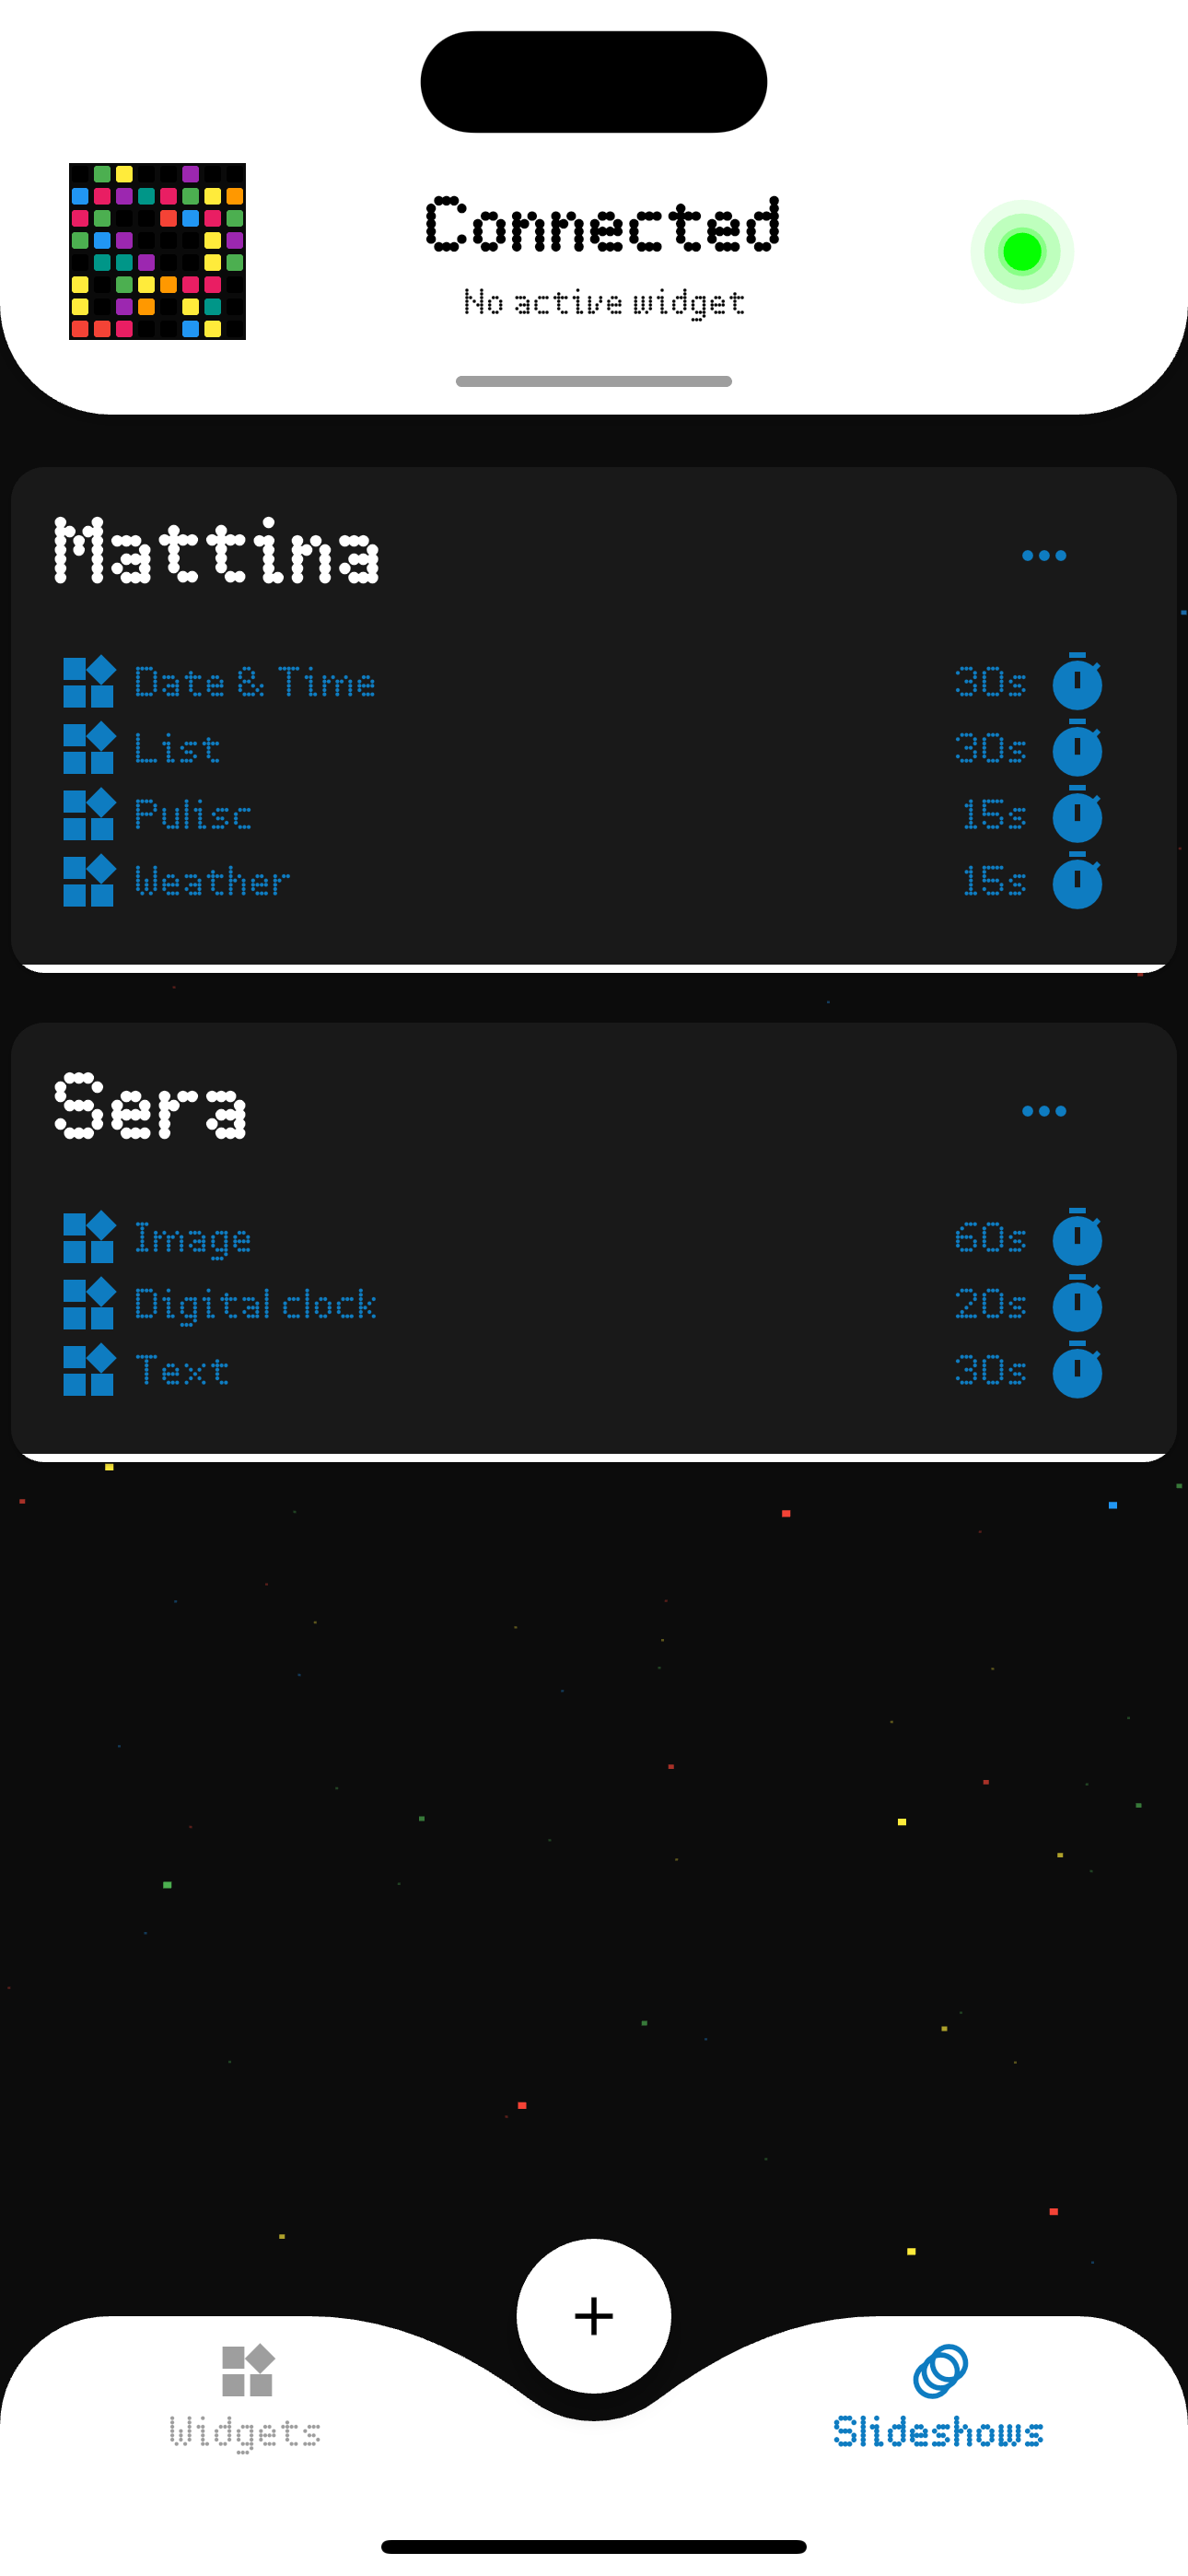
\includegraphics[width=\textwidth]{tesi/img/client_demo/slideshows/page.png}
        \caption*{Slideshows Page}
    \end{minipage}
    \begin{minipage}[b]{0.32\textwidth}
        \centering
        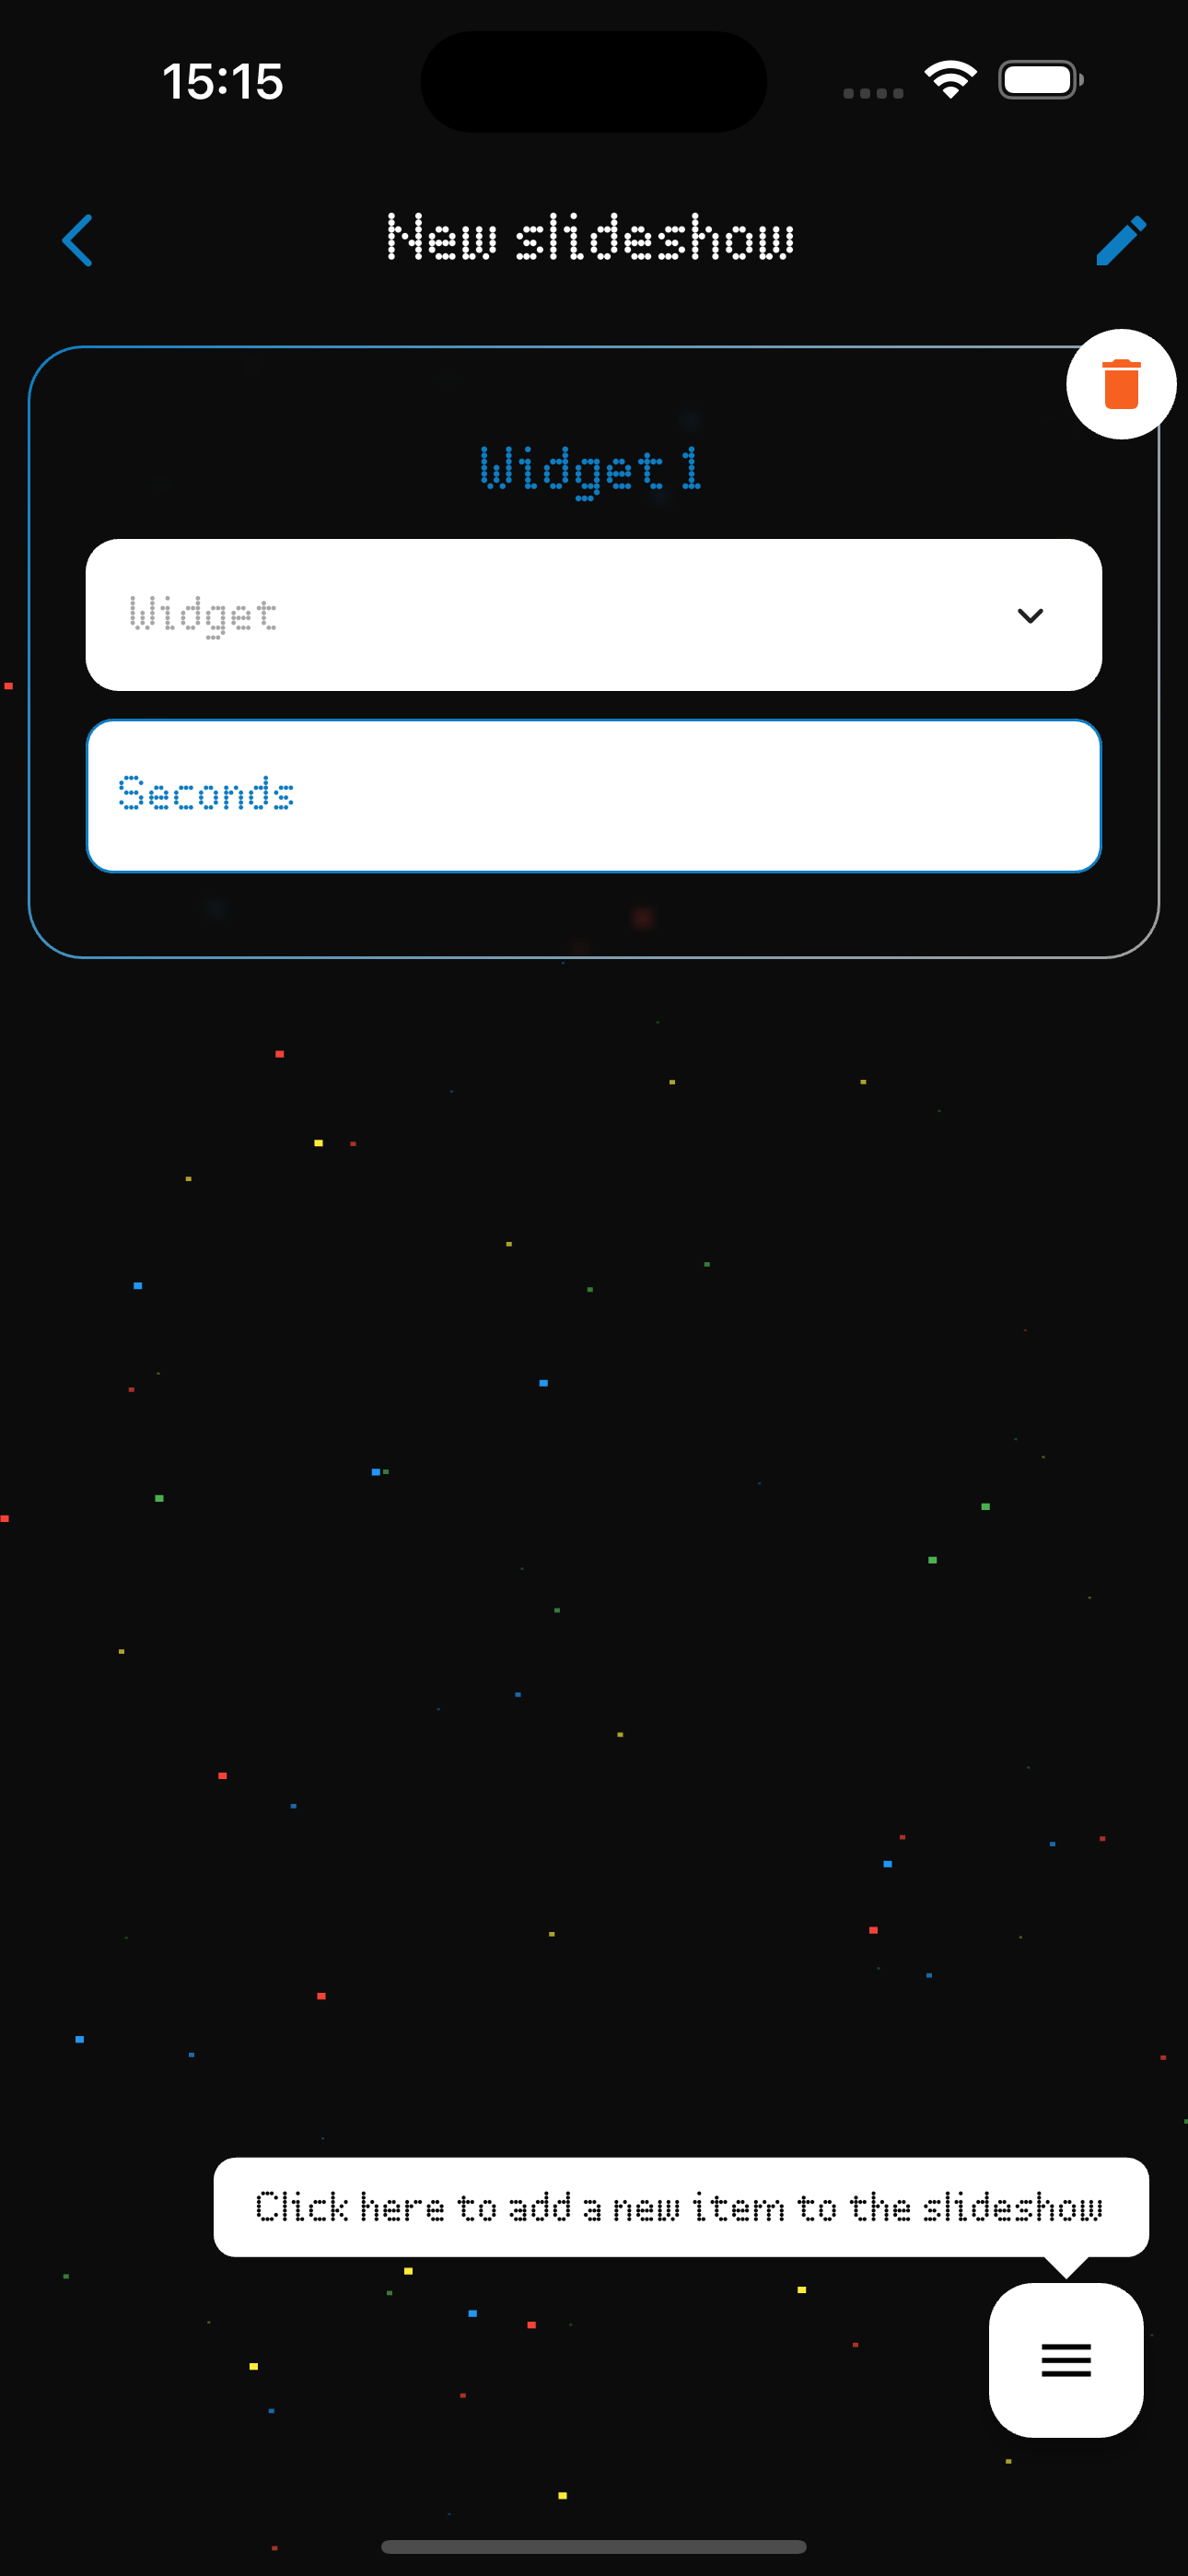
\includegraphics[width=\textwidth]{tesi/img/client_demo/slideshows/new.png}
        \caption*{Create a New Slideshow}
    \end{minipage}
    \begin{minipage}[b]{0.32\textwidth}
        \centering
        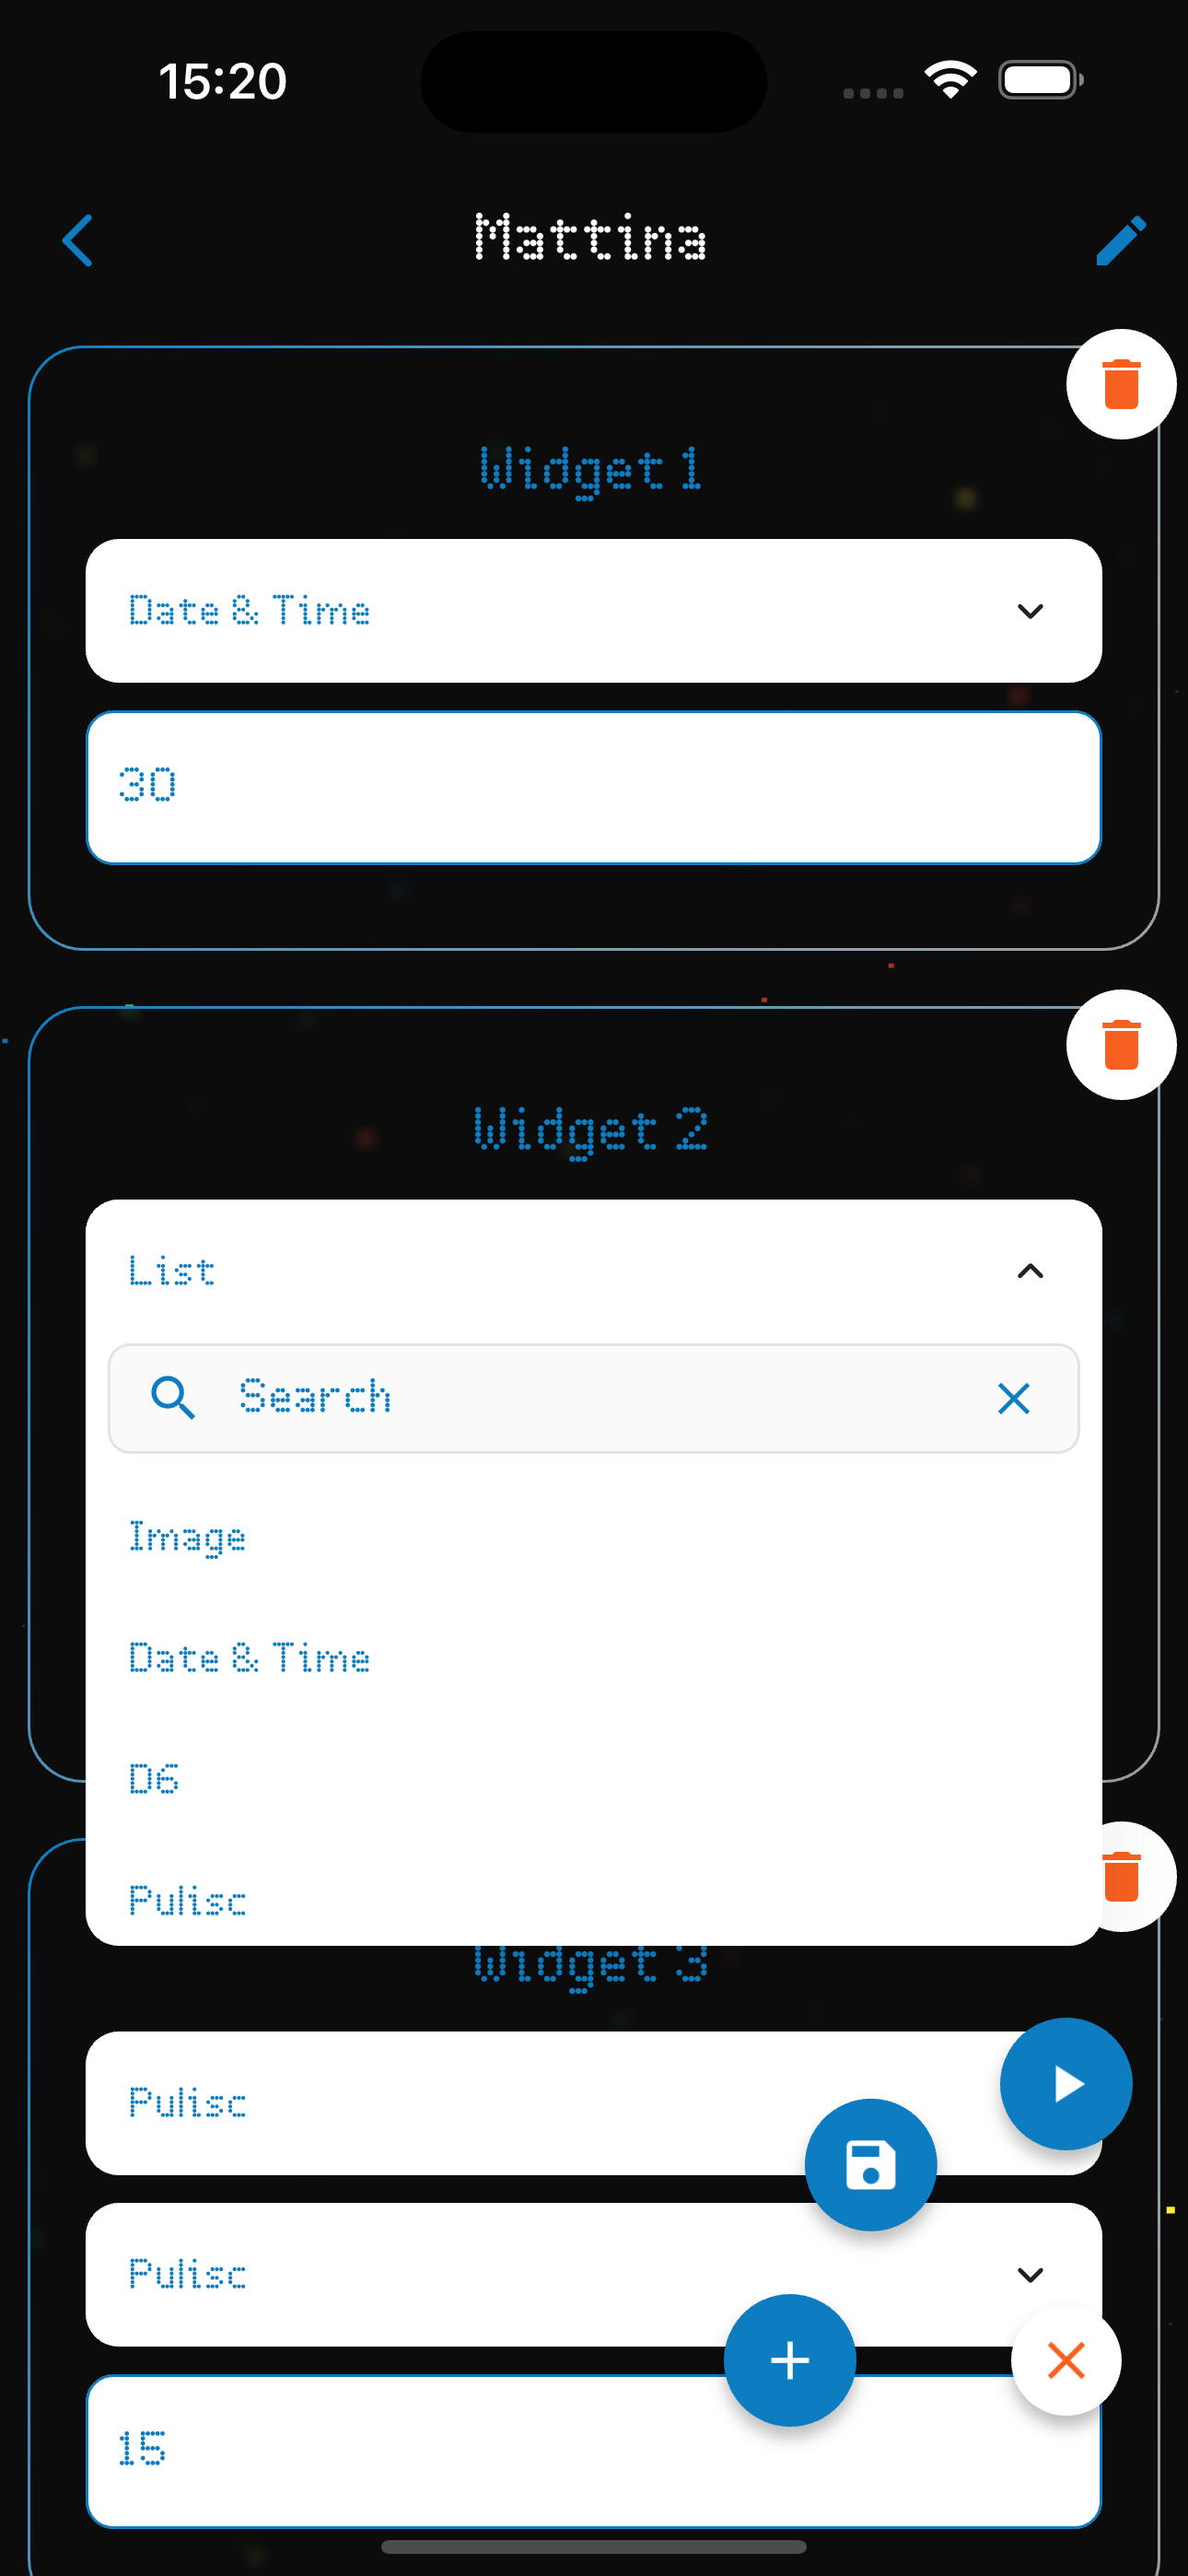
\includegraphics[width=\textwidth]{tesi/img/client_demo/slideshows/edit.png}
        \caption*{Edit an Existing Slideshow}
    \end{minipage}
\end{figure}

\section{Configuration Generator}
Configurable widgets \ref{widget-types} require a mechanism to collect data from users in order to configure the widget appropriately. 
Developers can create a configuration file in JSON format, which will be parsed by the configuration generator to dynamically create a form. 
This form allows the user to input the necessary data to configure the widget.

This design decision was crucial to ensuring that developers could create new widgets without needing to concern themselves with user interface design, while also maintaining consistency in the configuration process across widgets from different developers.

\subsection{Example}

A simple example of a configuration file to display a list of items is shown below:

\begin{minipage}{0.45\textwidth}
\begin{minted}{json}
{
  "form": {
    "title": "Shopping List",
    "description": "Configure your 
    widget here",
    "fields": [
      {
        "name": {
          "type": "string",
          "label": "Name",
          "required": true,
          "placeholder": "Enter the 
          name of this list"
        },
        "color": {
          "type": "color",
          "label": "Color",
          "required": true,
          "placeholder": "Choose the 
          color of the title"
        },
        "items": {
          "type": "string[]",
          "label": "Shopping items",
          "required": true,
          "placeholder": "Insert your 
          items here"
        }
      }
    ]
  }
}
\end{minted}
\end{minipage}
\hfill
\begin{minipage}{0.45\textwidth}
\centering
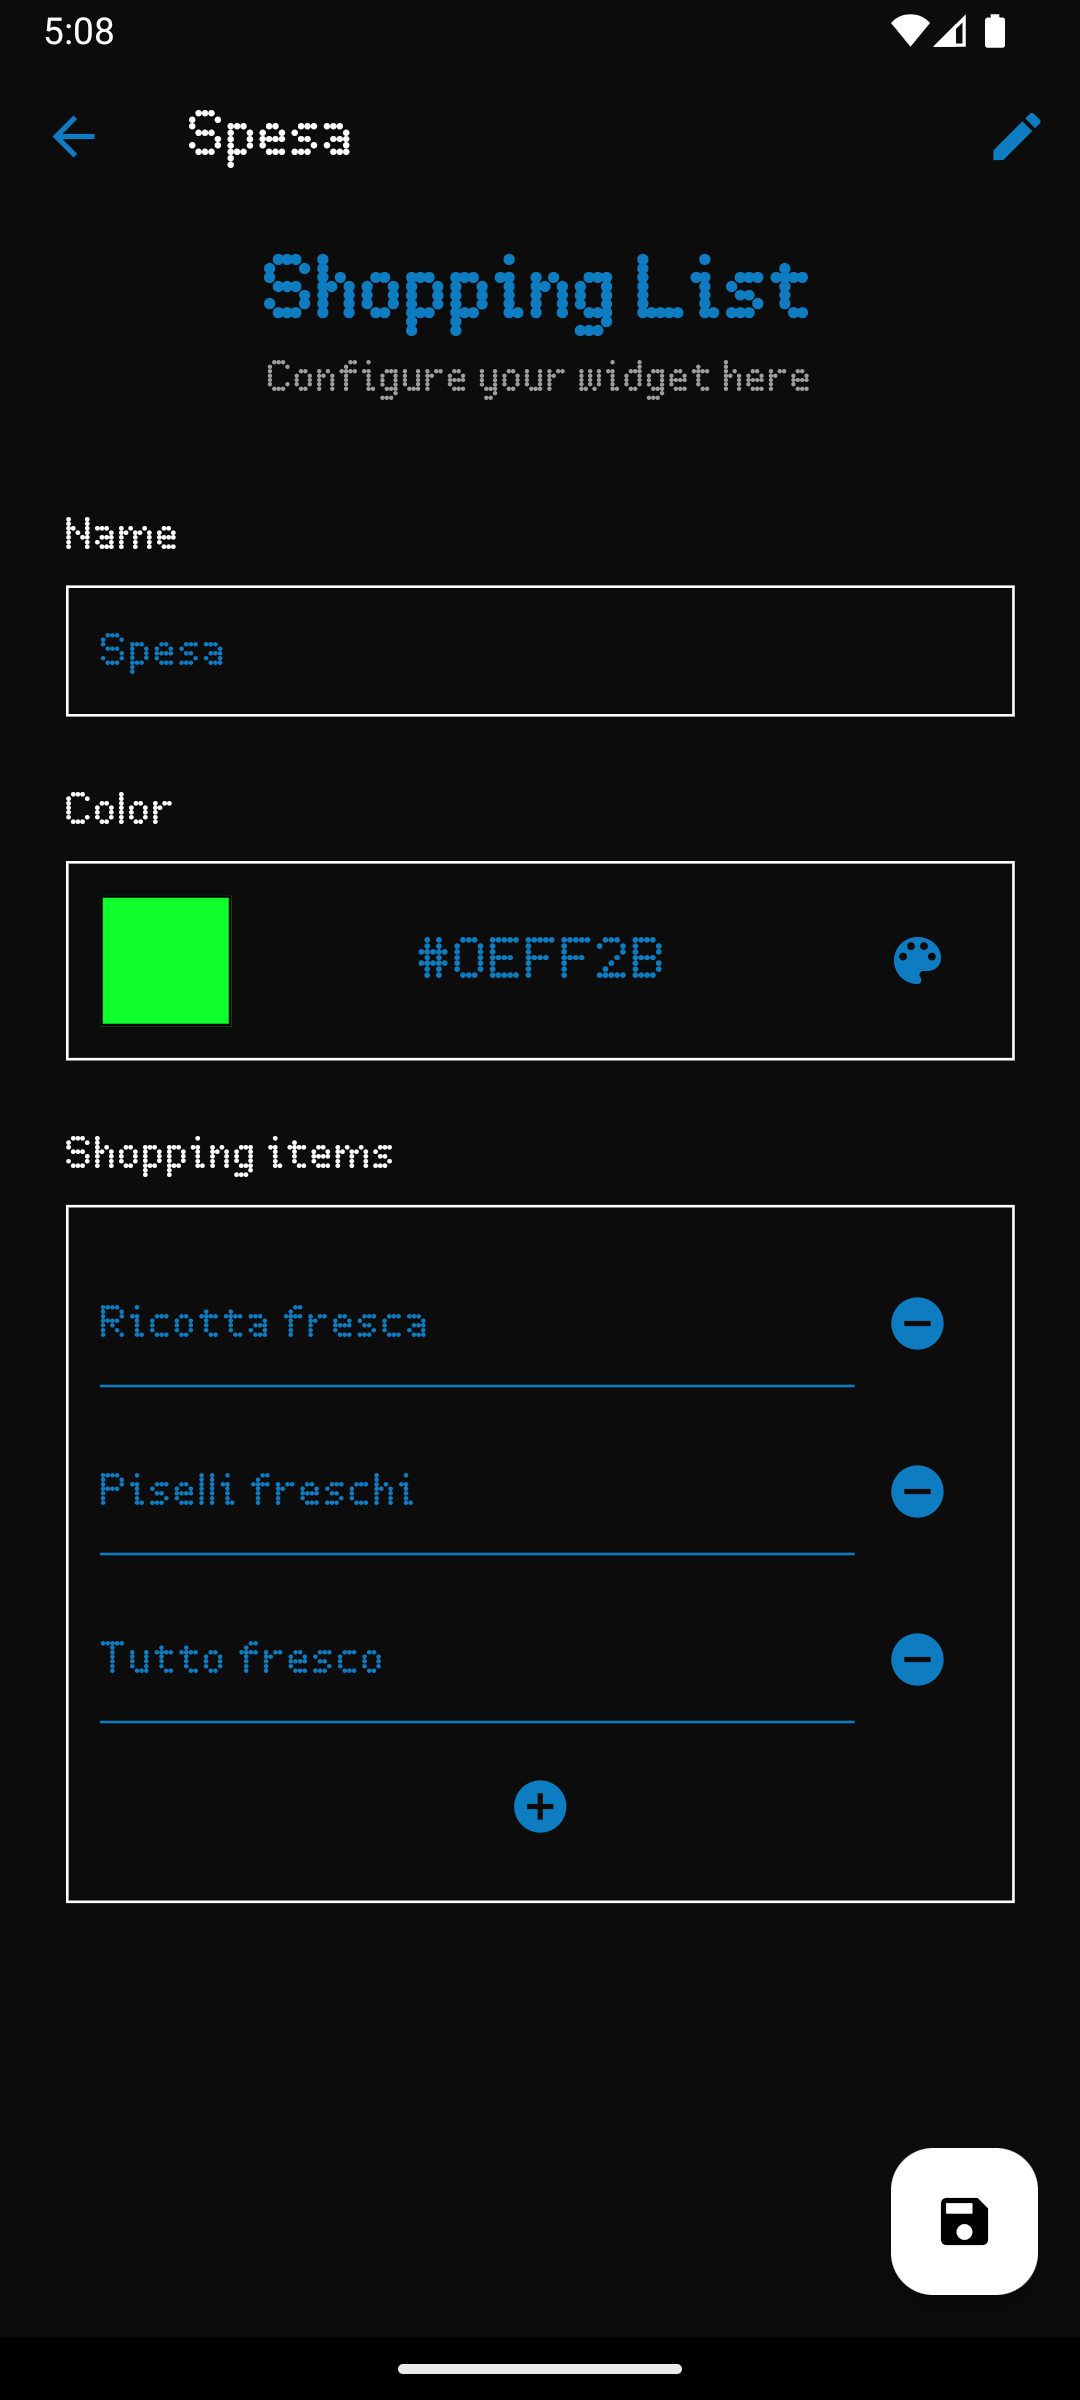
\includegraphics[width=\textwidth]{tesi/img/config_form/shopping_list_form.png}
\captionof{figure}{Client rendered form}
\end{minipage}

\subsection{Result of the Configuration}
The data collected from the user through the configuration form is saved in a JSON file. 
This file is parsed by the C++ engine when the specific widget with that configuration is loaded. 
Accessing the data from the configuration is straightforward in Python, as illustrated by the following example:

\begin{minipage}{0.65\textwidth}
\begin{minted}{python}
# config contains all the data from the configuration
from mosaico import widget, config

# Create title
text = widget.createText()
text.setText(config["name"])
text.setHexColor(config["color"])
text.moveTo(2,0)
text.setFont("9x18")

# Create items
items = []
bullets = []
for i in range(0, len(config["items"])):
    # Create bullet
    bullets.append(widget.createRectangle())
    bullets[i].setSize(2,2)        
    bullets[i].moveTo(4,16)
    bullets[i].translateYBy((i*7) + 5)    
    bullets[i].setHexColor(config["color"])  
    
    # Create entry  
    items.append(widget.createText())
    items[i].setFont("4x6")
    items[i].setText(config["items"][i])
    items[i].moveTo(8,14)    
    items[i].translateYBy((i*7) + 5)

def loop():
    pass
\end{minted}
\end{minipage}
\begin{minipage}{0.30\textwidth}
\centering
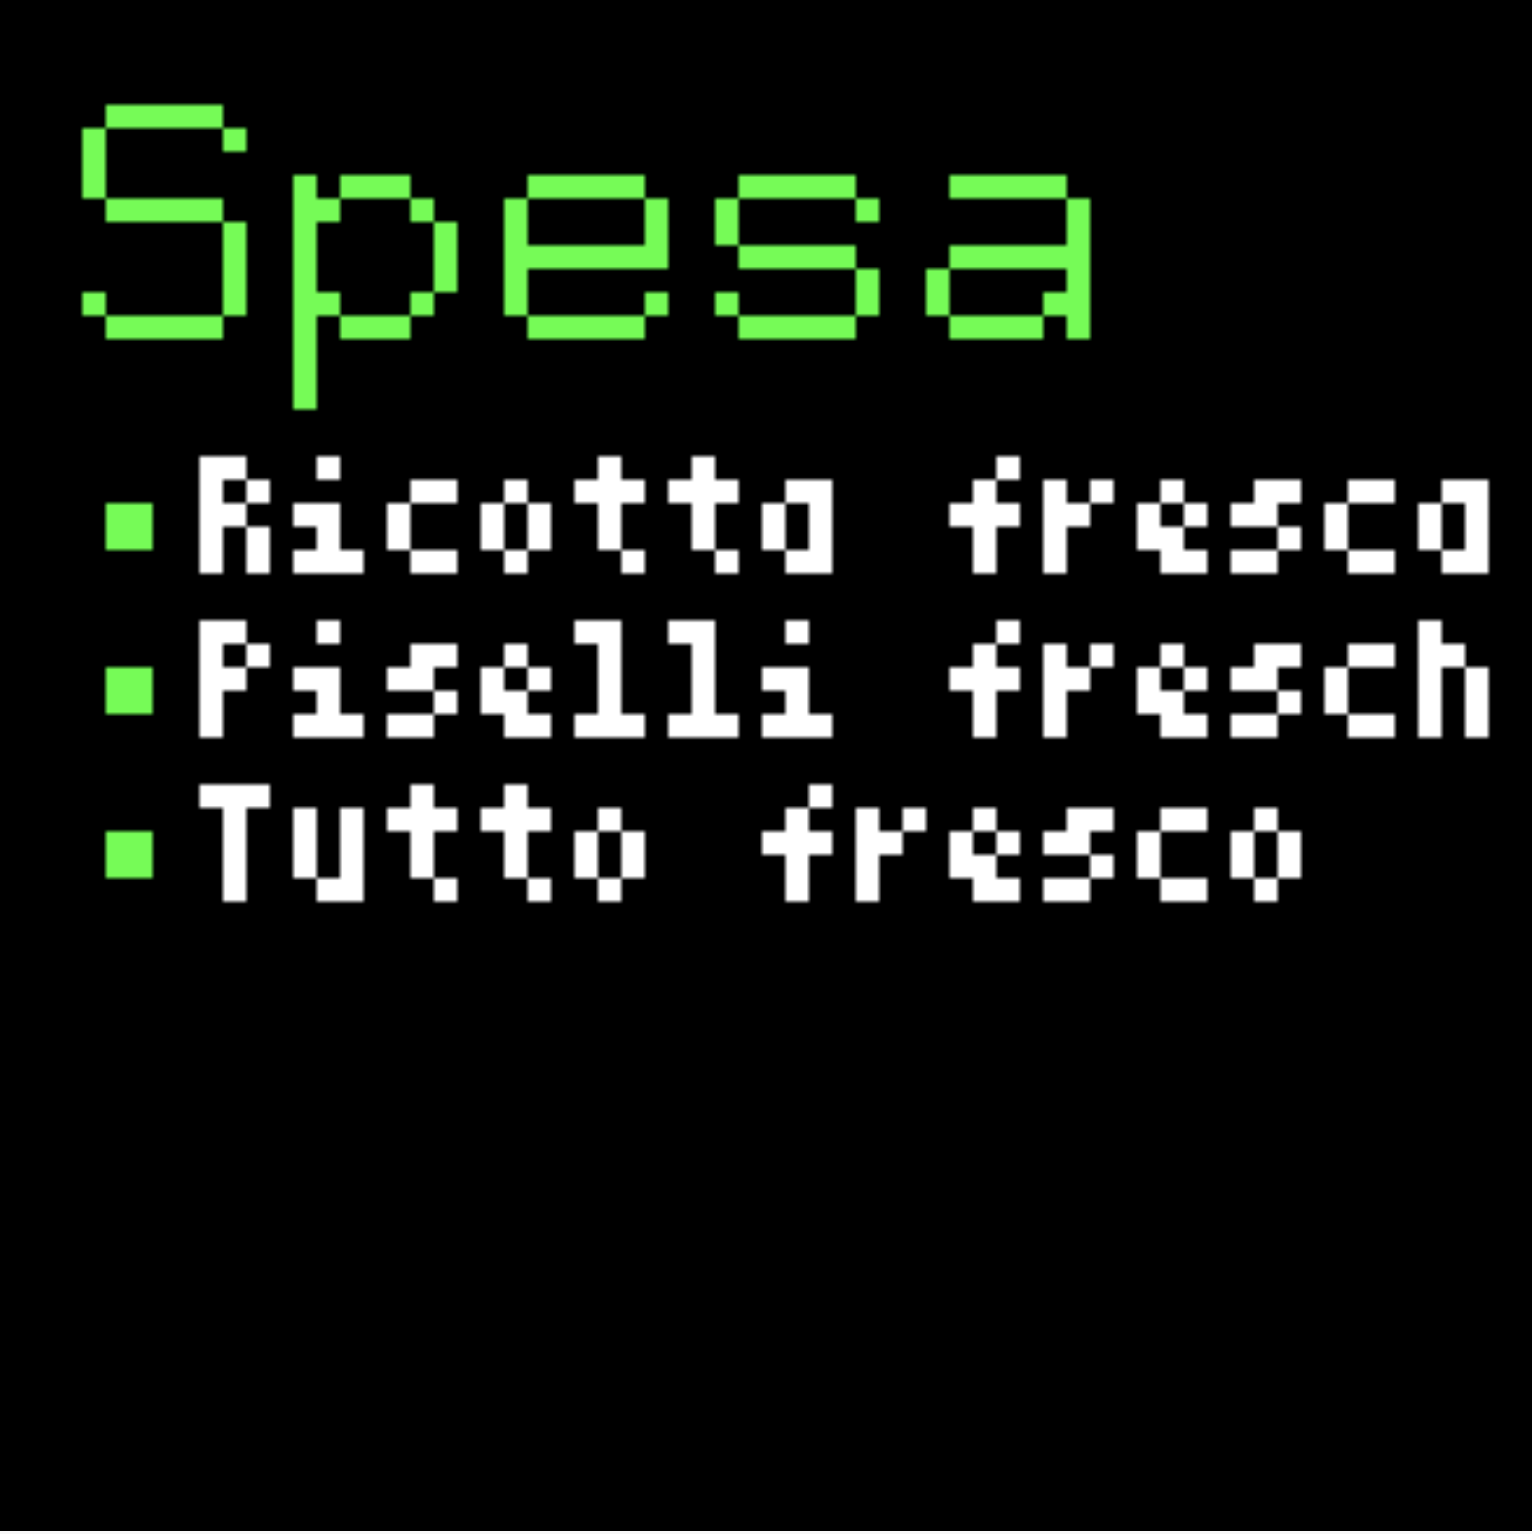
\includegraphics[width=\textwidth]{tesi/img/config_form/shopping_list_result.png}
\captionof{figure}{Result on matrix}
\end{minipage}

\subsection{Assets Management}
Each widget configuration is stored as a \texttt{.tar.gz} archive, which is essentially a compressed file that contains all the data submitted by the user. This compression facilitates faster transfers. Inside the archive, there is a \texttt{.json} file that holds the configuration details, as well as any additional binary files (e.g., images or other assets) uploaded by the user. A helper function is available to easily retrieve the path to these assets within the archive, simplifying access to the resources when needed.

\subsection{Field Attributes}
All fields share the following common attributes, regardless of their type:

\begin{itemize}
    \item \textbf{Name (required):} The unique identifier for the field within the configuration file. \textbf{Note:} \textit{You cannot use the same name for different fields}

    \item \textbf{Type (required):} Specifies the data type of the field. The type can be one of the following:
    \begin{itemize}
        \item \texttt{string}: A simple text field.
        \item \texttt{string[]}: An array of strings.
        \item \texttt{color}: A color picker field.
        \item \texttt{image}: An image upload field.
            \textbf{Special Attributes:}
            \begin{itemize}
            \item \texttt{Dimensions}: Specifies the image dimensions, as an object containing:
            \begin{itemize}
                \item \texttt{width}: The image width in pixels.
                \item \texttt{height}: The image height in pixels.
            \end{itemize}
            \end{itemize}
        \item \texttt{select}: An font selector between one of the available.
        \textbf{Special Attributes:}
            \begin{itemize}
            \item \texttt{options}: An array of strings, one will be selected by the user
            \end{itemize}
        \item \texttt{font}: An font selector between one of the available.
    \end{itemize}

    \item \textbf{Label:} The label displayed to the user in the configuration form to help them understand the purpose of the field.

    \item \textbf{Required:} A boolean value that indicates whether the field is mandatory.

    \item \textbf{Placeholder:} A placeholder text shown when the field is empty, providing guidance to the user about what to enter.
\end{itemize}


\subsection{Multiple configurations}
Obviously it would not make sense to create a configuration for one use only, once a configuration for a specific widget is created and user gave it a name, it will always be possible for them to list all the created, delete them or edit them using the appropriate 

\section{Device Discovery}
One of the essential features of the application is the automatic discovery mechanism, enabling seamless connectivity to a matrix device without requiring complex setup or manual configuration. The goal is to ensure that the application can autonomously identify and connect to any available matrix nearby.

Communication with the matrix device is handled through CoAP. However, in order to initiate this communication, the application must first obtain the IP address of the Raspberry Pi hosting the matrix. To address this challenge, a BLE GATT server is set up alongside the CoAP server. The GATT server exposes a service named \textit{Mosaico}, identified by a constant UUID, which the application can use to recognize the presence of a matrix. A simple BLE scan allows the application to detect this service and establish a connection.

The following algorithm outlines the process for automatically discovering and connecting to a matrix:

\begin{algorithm} \caption{Device discovery}\label{alg
} \begin{algorithmic} \Ensure Returns the matrix IP if successfully pinged, or \texttt{null} if all attempts fail

\State $prefs \gets \text{get preferences instance}$ \State $lastKnownMatrixIp \gets \text{get stored value from prefs}$ \If{$lastKnownMatrixIp \neq null$ \textbf{and} \texttt{pingMatrix}($lastKnownMatrixIp$)} \State \Return $lastKnownMatrixIp$ \EndIf

\If{\texttt{not} BLEDeviceConnected()} \State \texttt{searchAndConnectBleDevice()} \Comment{Attempt BLE connection} \EndIf

\State \texttt{ensureBleDeviceConnected()} \State $ipFromBle \gets \texttt{matrixBleService.getMatrixIp()}$ \If{$ipFromBle \neq null$ \textbf{and} \texttt{pingMatrix}($ipFromBle$)} \State \texttt{prefs.setString('matrixIp', ipFromBle)} \State \Return $ipFromBle$ \EndIf

\State \Return \texttt{null} \end{algorithmic} \end{algorithm}

If the automatic discovery process is unsuccessful, users can manually set the matrix IP address via the \textit{Set Manual Matrix Address} option in the device control panel, allowing them to connect to the matrix manually.

\section{Caching}
The constrained capabilities of the Raspberry Pi Zero W represent the primary limitation in the Mosaico ecosystem. While its core function is to render dynamic content on the LED matrix, it also operates as both a COAP and BLE server, facilitating communication with the mobile application. The dual responsibilities placed on the Pi necessitate careful management of system resources to avoid overburdening the device, particularly when handling frequent network requests.

To mitigate unnecessary strain on the Raspberry Pi, Mosaico employs efficient caching mechanisms within the mobile client. This reduces redundant calls to the COAP server, especially for frequently accessed data such as installed widgets, created slideshows, and widget configurations. The caching strategy is straightforward yet effective: commonly requested services are retrieved once, typically when users initially open the app or navigate to specific sections that trigger those requests. Subsequent interactions with these services do not require re-querying the COAP server unless there is a change, such as the installation of a new widget. In such cases, the cache is intelligently updated in memory without fully refreshing the entire dataset.

The use of caching not only improves the user experience by speeding up interactions but also reduces the overall communication overhead on the Raspberry Pi, ensuring that its limited resources are efficiently utilized. By implementing an in-memory cache for frequently accessed data, Mosaico reduces the need for repetitive data fetching, which would otherwise place undue load on the system. This approach ensures the platform remains responsive, even on the resource-constrained Raspberry Pi Zero W.

From a broader perspective, this resource-conscious design exemplifies how careful consideration of hardware limitations can be balanced with software optimizations to maintain system performance. By integrating caching strategies, Mosaico achieves a more scalable solution while prolonging the lifespan and effectiveness of the hardware within the IOT ecosystem.

\section{Design Patterns}
In the mobile application development of Mosaico, the \textbf{BLoC (Business Logic Component)} design pattern was utilized to manage and maintain the app's state in a scalable and organized manner. The separation of concerns provided by BLoC ensures that the UI reacts to changes in the app's state efficiently, promoting cleaner, testable, and maintainable code.

BLoC acts as the intermediary between the UI and the business logic of the application, where each BLoC listens to \textbf{events} and emits corresponding \textbf{states}. This makes it ideal for applications where user interactions and changes in data need to be reflected dynamically across different parts of the UI.

\subsection{BLoC for Installed Widgets Feature}

An excellent example of BLoC in action can be seen in the \textbf{Installed Widgets Page}. This page showcases widgets that users have installed on their LED matrix devices. Using a combination of \textbf{BlocListeners} and \textbf{BlocBuilders}, the UI dynamically updates based on external events such as matrix connections or widget store interactions.

\begin{minted}{dart}
return MultiBlocListener(
  listeners: [
    BlocListener<MatrixDeviceBloc, MatrixDeviceState>(
      listener: (context, state) {
        // Only refresh installed widgets if connected to a new matrix
        if (state is MatrixDeviceConnectedState && state.newConnection) {
          context.read<MosaicoInstalledWidgetsBloc>()
              .add(LoadInstalledWidgetsEvent());
        }
      },
    ),
    BlocListener<MosaicoStoreBloc, MosaicoStoreState>(
      listener: (context, state) {
        // Refresh when new widgets are available from the store
        if (state is MosaicoStoreLoadedState) {
          context.read<MosaicoInstalledWidgetsBloc>()
              .add(LoadInstalledWidgetsEvent());
        }
      },
    ),
  ],
  child: BlocBuilder<MosaicoInstalledWidgetsBloc, MosaicoInstalledWidgetsState>(
    builder: (context, state) {
          // Handle different states (Loading, Loaded, Error)
          // and provide the appropriate UI response.
          
          // Loading
          if (state is MosaicoInstalledWidgetsLoading) {
            return Center(child: Center(child: LoadingMatrix()));
          }

          // Loaded
          if (state is MosaicoInstalledWidgetsLoaded) {
           if (state.installedWidgets.isEmpty) {
              return const EmptyPlaceholder(
                  hintText: "No widgets? Install some from the store!");
            }
            // Show installed widgets tiles
          }

          // Error
          if (state is MosaicoInstalledWidgetsError) {
            return EmptyPlaceholder(
              hintText: state.message,
              onRetry: () {
                context
                    .read<MosaicoInstalledWidgetsBloc>()
                    .add(LoadInstalledWidgetsEvent());
              },
            );
          }

          // Not connected?
          return const EmptyPlaceholder(
              hintText: "Connect to matrix to see installed widgets");
    },
  ),
);
\end{minted}

In this code, the \textbf{InstalledWidgetsPage} listens for events from multiple BLoCs:

\begin{itemize}
    \item \textbf{MatrixDeviceBloc} triggers updates when a new connection is made to an LED matrix device.
    \item \textbf{MosaicoStoreBloc} listens for changes in the widget store, refreshing the installed widgets list when new widgets are available for installation.
\end{itemize}

This dynamic reaction between BLoCs allows different parts of the app to remain in sync, minimizing redundant requests and ensuring that data is updated only when necessary.

\subsection{BLoC for Widget Store Interactions}

In the \textbf{Mosaico Store}, when a user installs a new widget, the \textbf{MosaicoStoreBloc} processes this event by calling the appropriate repository to handle the widget installation. Once completed, the store emits an updated state that is listened to by other components, like the \textbf{Installed Widgets Page}, so the newly installed widget appears without additional user action.

This interaction emphasizes the power of BLoC to coordinate state changes across different sections of the app. When a new widget is installed, the state is updated across all relevant UI components in real-time.

By employing the BLoC pattern, the app benefits from a well-structured and responsive design where state changes in one area, such as the widget store, can immediately reflect in another, like the list of installed widgets. This approach reduces unnecessary API calls and ensures the app provides an efficient user experience.

This section highlights the practical advantages of the BLoC pattern, reinforcing its role in handling complex state management tasks in a clean and modular way.

\chapter{The Cloud}
For the back-end side of my application, I chose a tech stack that I thoroughly enjoy working with: Laravel, MariaDB, and Filament, all fully dockerized and running on an Ubuntu VM hosted on my personal home server.

\begin{itemize}
    \item Laravel: As a PHP framework, Laravel offers a robust and elegant solution for building scalable, secure, and maintainable back-end applications. It provides built-in features like routing, ORM (Eloquent), middleware, and more, allowing me to focus on the business logic of Mosaico rather than boilerplate code.
    \item MariaDB: For the database, I selected MariaDB because it is a community-developed fork of MySQL and provides excellent performance, scalability, and open-source benefits. Its compatibility with MySQL made it a straightforward choice for integration with Laravel's Eloquent ORM.
    \item Filament: As an admin panel generator, Filament enables me to create highly interactive admin interfaces with minimal effort. It integrates seamlessly with Laravel, allowing me to manage widgets and user data from a sleek UI while offering powerful tools like forms, tables, and resource management.
    \item Dockerization: To ensure the application is easy to maintain and deploy, I containerized the entire stack using Docker. Dockerization provides isolation for each component and eliminates the "it works on my machine" problem by creating consistent environments across development and production.
    \item Ubuntu VM: The server runs on an Ubuntu virtual machine hosted on my personal home server. This setup gives me full control over the deployment process and allows for flexibility in configuring and maintaining the environment.
\end{itemize}

This stack not only aligns with my technical preferences but also ensures that Mosaico's back-end is scalable, flexible, and easy to manage, making it a solid foundation for the future development of the platform.

\section{Widget manager}
The Widget Manager serves as the portal through which developers can contribute their widgets to the community by uploading them to the store. To streamline the onboarding process, account creation and widget submission are facilitated by a simple "Sign in with GitHub" option, requiring only a single tap to initiate. This reduces friction and ensures ease of access for new contributors.

Upon signing in, developers gain immediate access to their dashboard, where they can view a list of previously developed widgets, create new ones, or modify existing submissions.

\begin{figure}[h] \centering \begin{minipage}[b]{0.49\textwidth} \centering 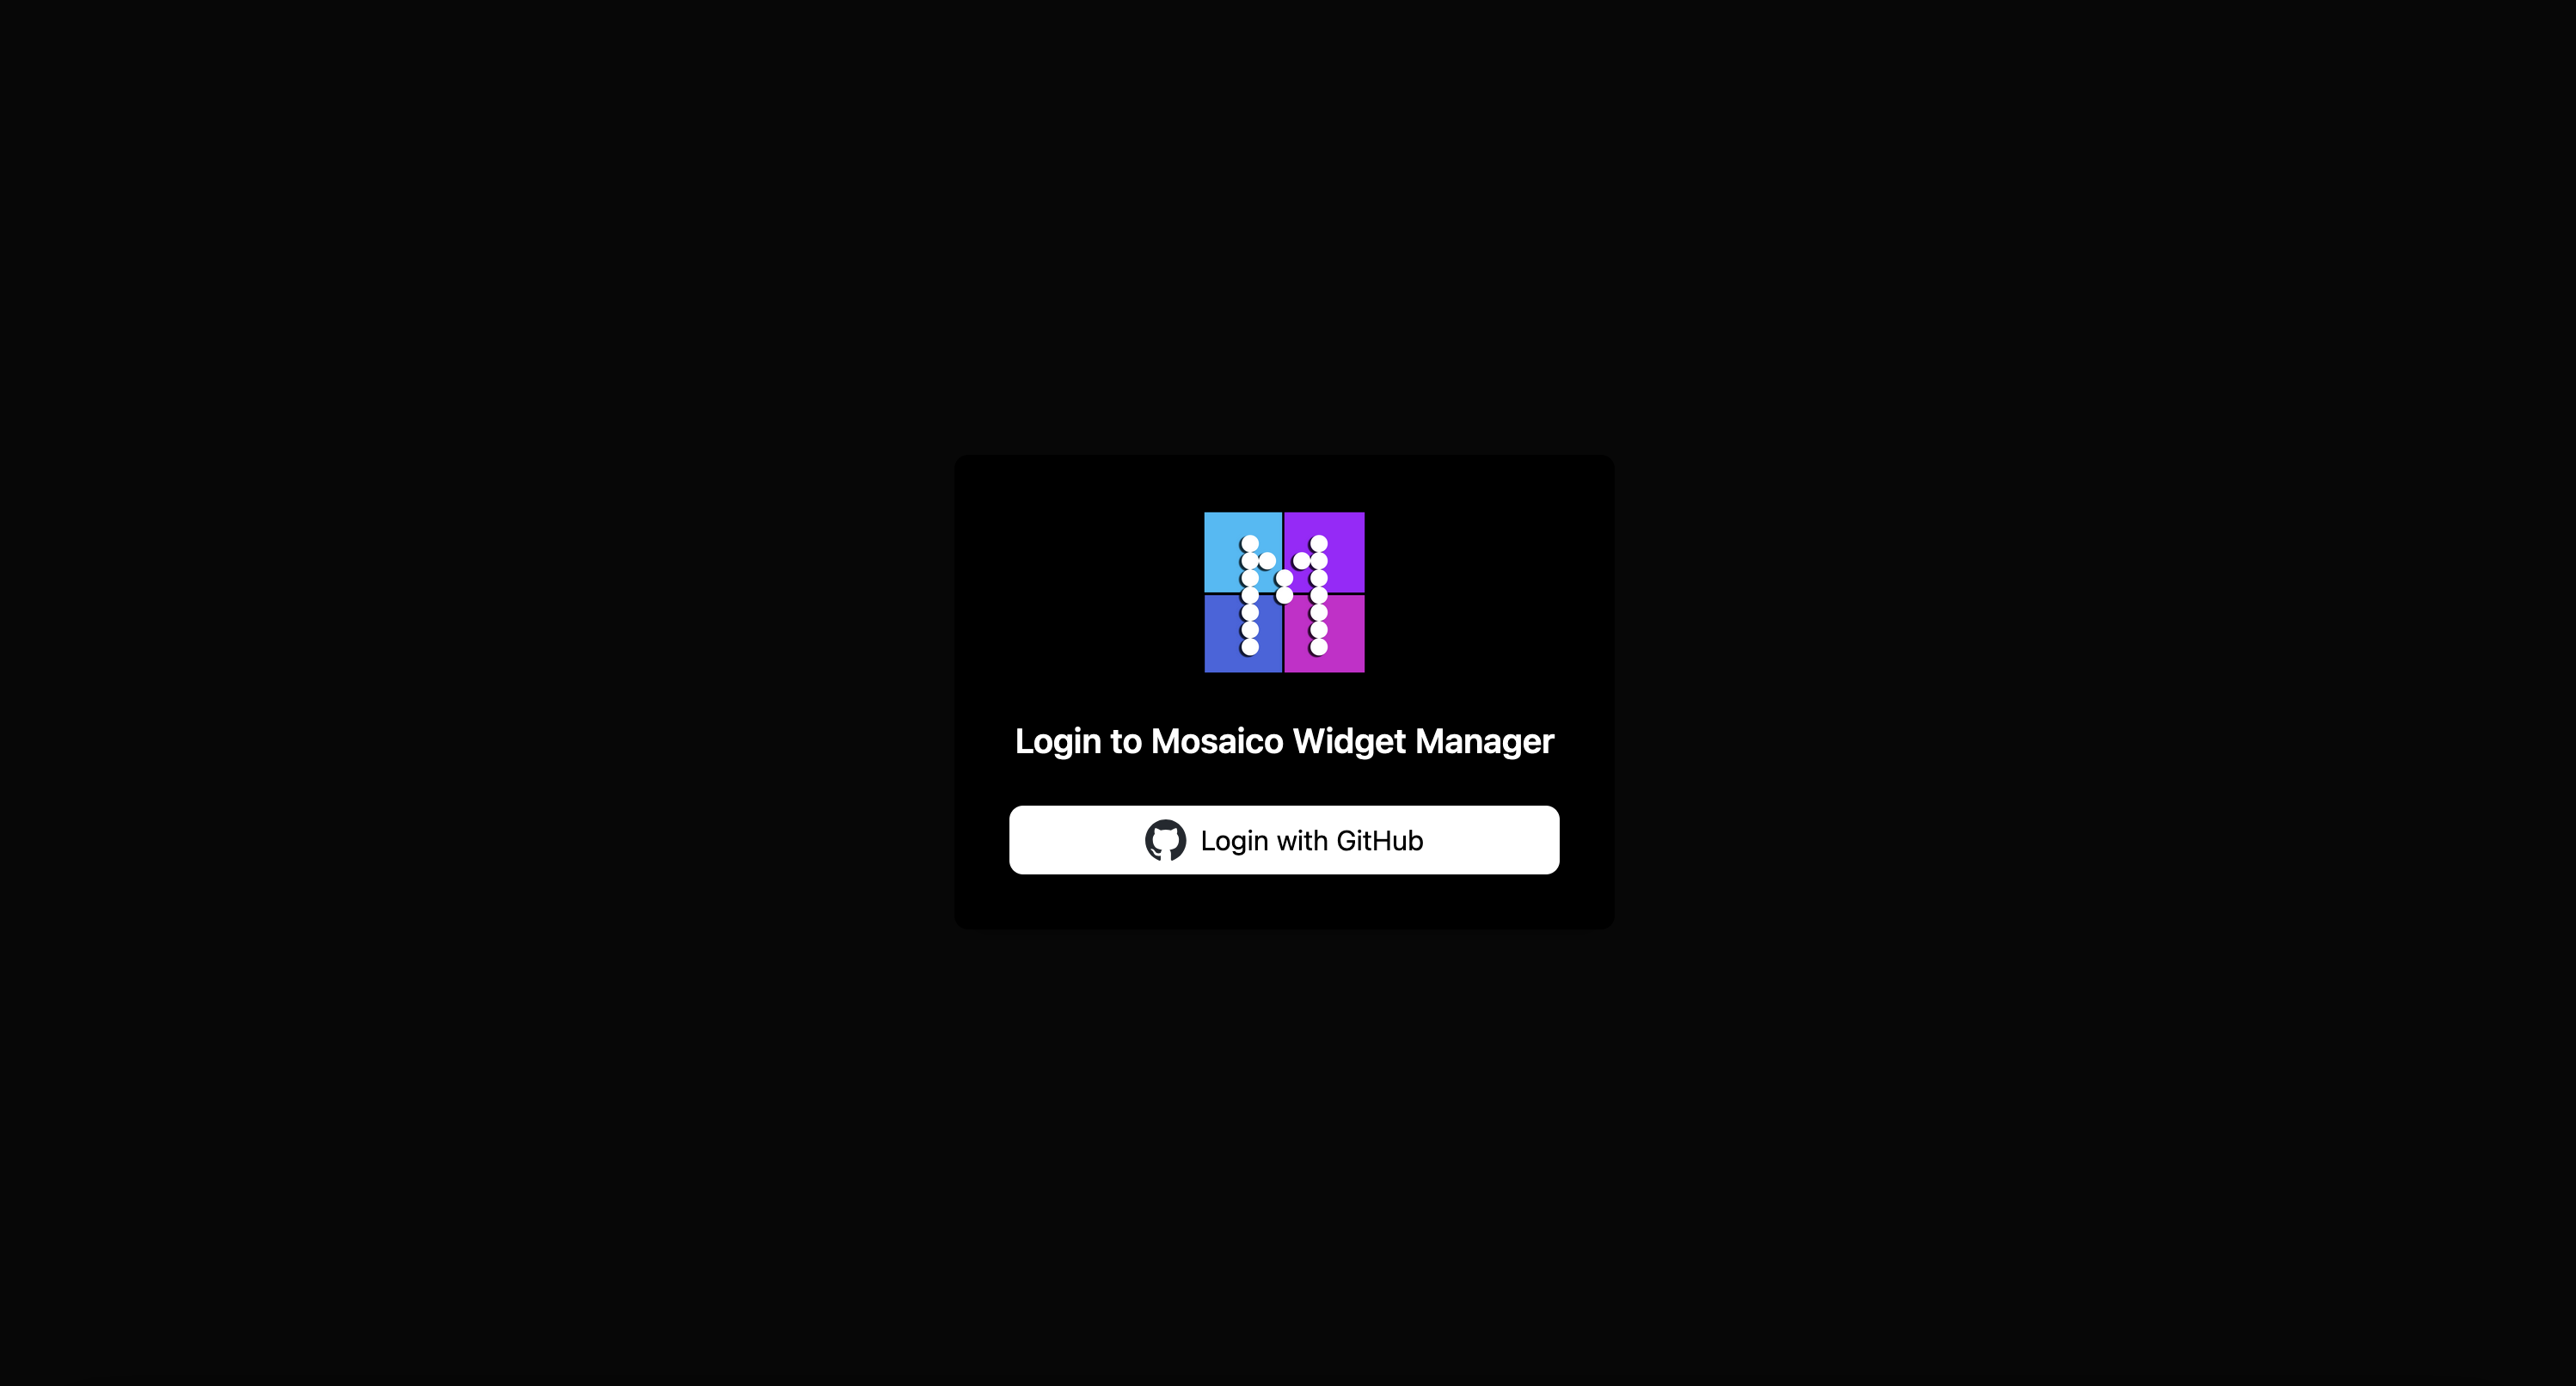
\includegraphics[width=\textwidth]{tesi/img/website_demo/login.png} \caption*{Login with GitHub} \end{minipage} \begin{minipage}[b]{0.49\textwidth} \centering 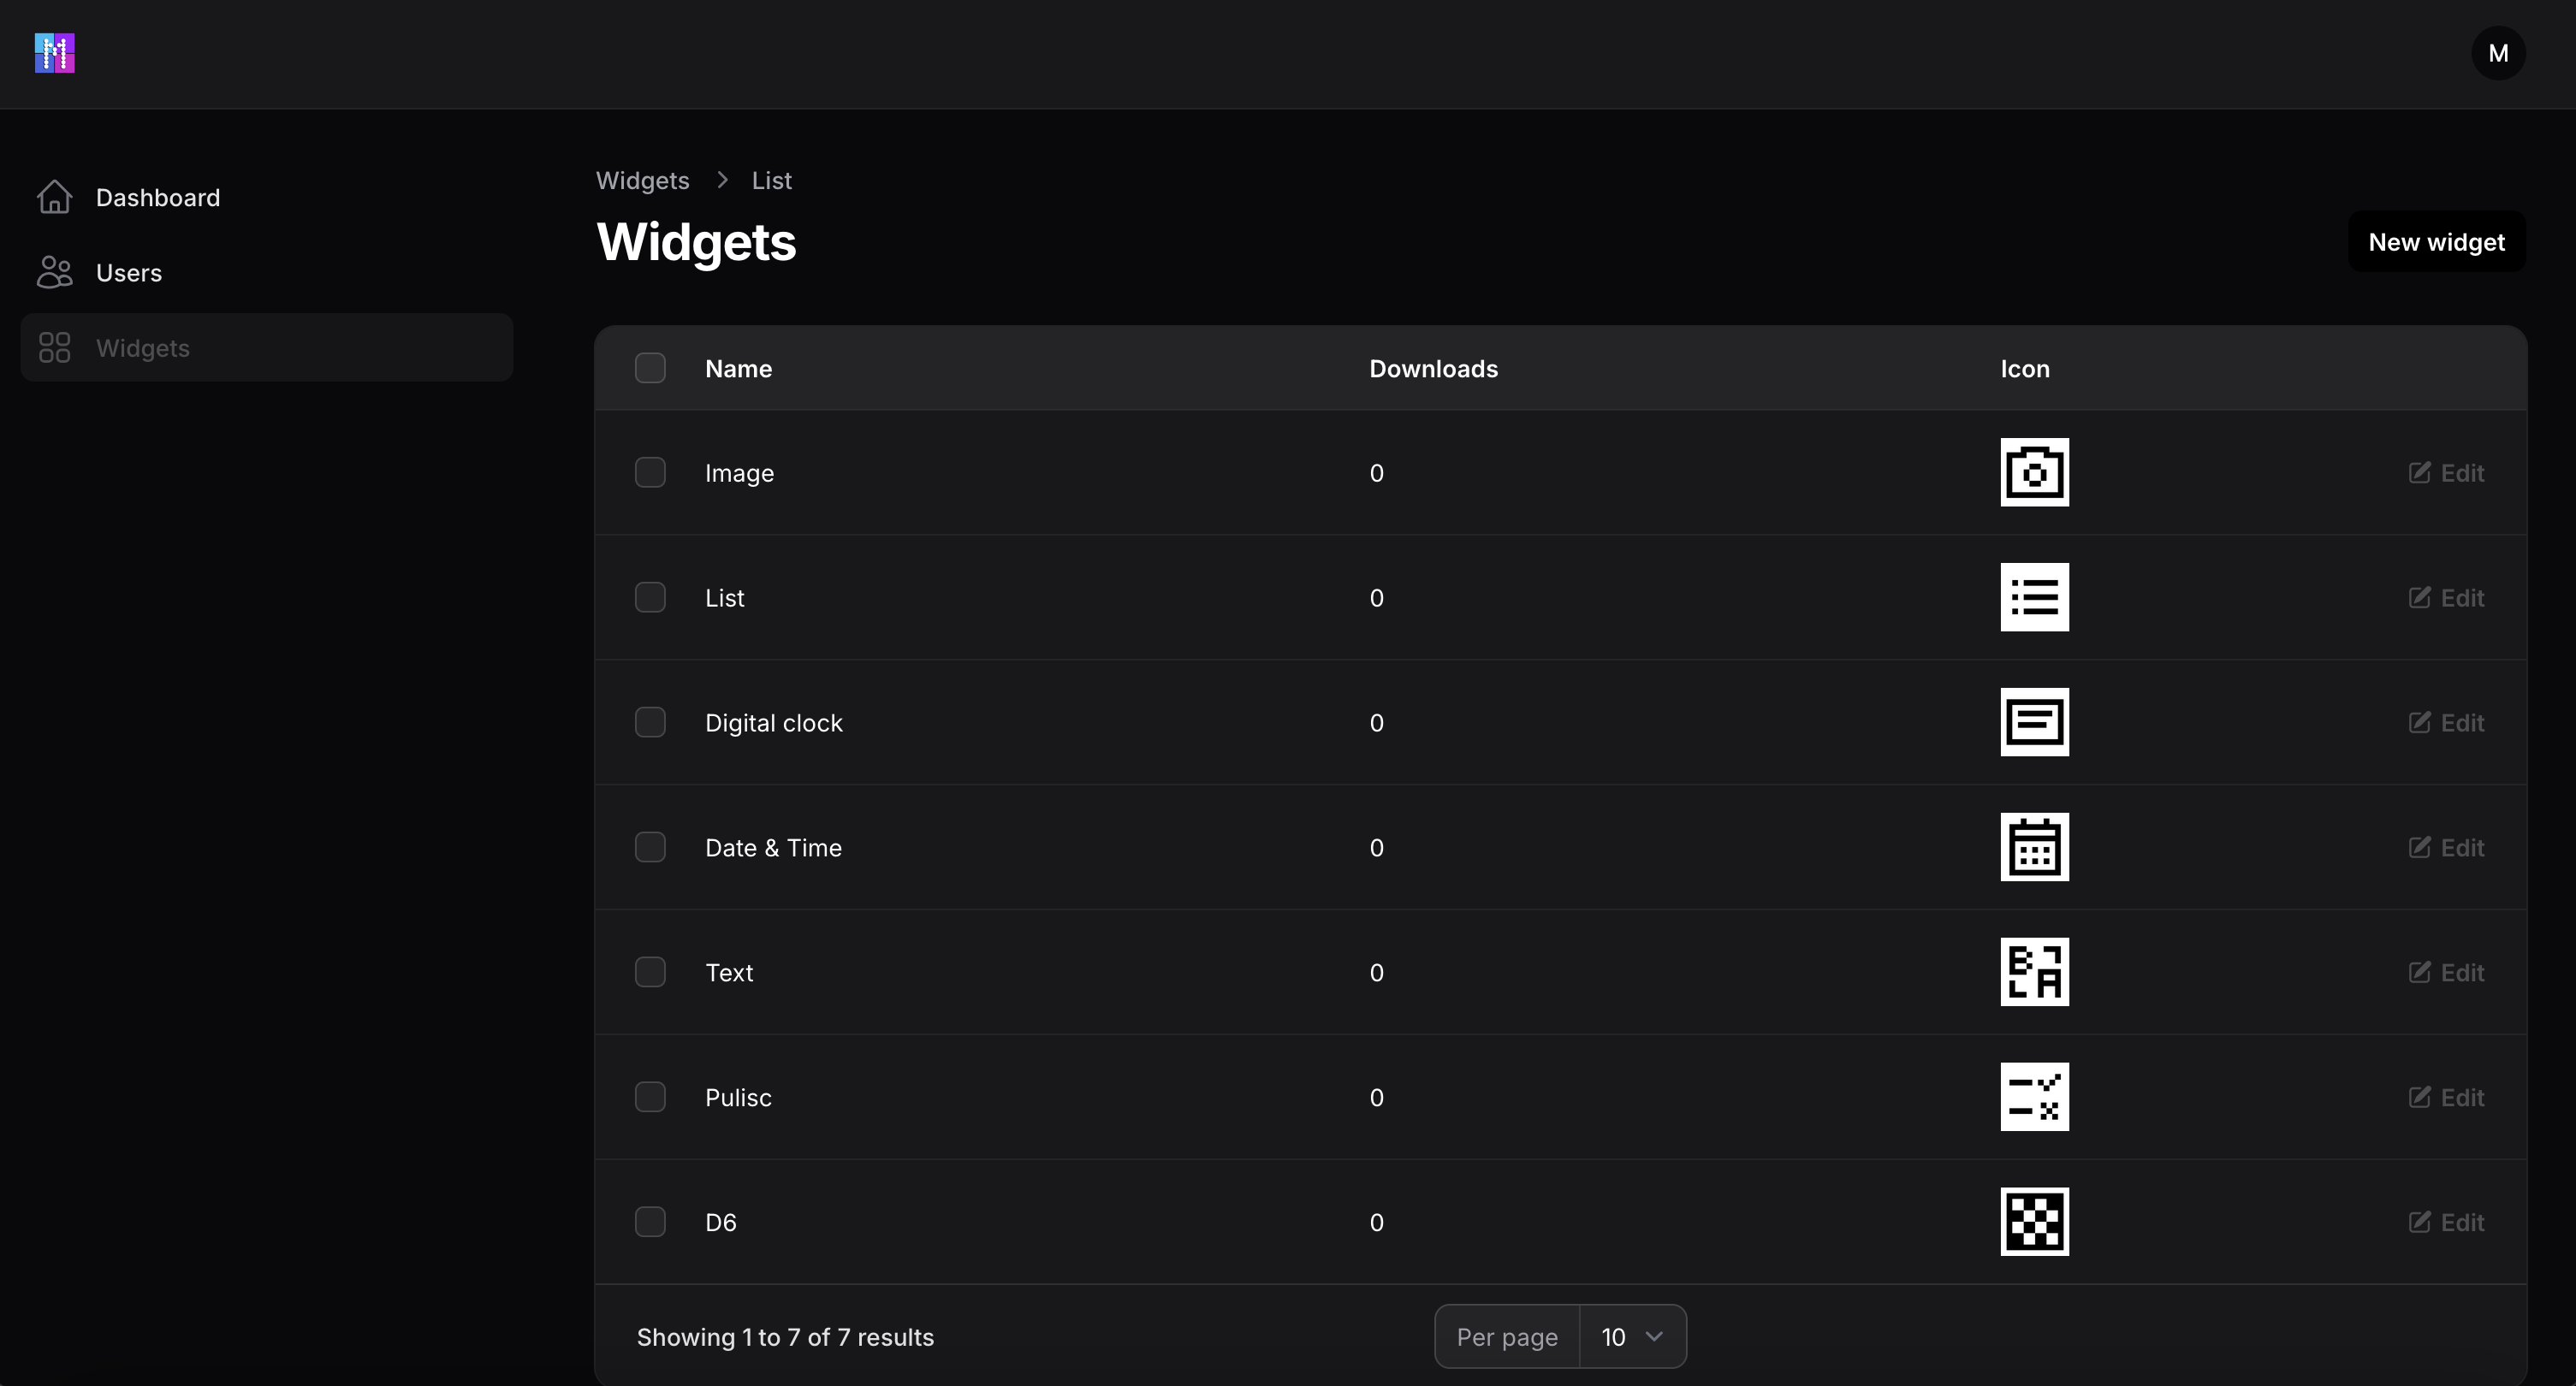
\includegraphics[width=\textwidth]{tesi/img/website_demo/widgets.png} \caption*{Developer's Widgets} \end{minipage} \end{figure}

The user interface has been designed to be intuitive and accessible, ensuring that developers can easily manage their contributions. Developers are required to provide the following information for each widget submission:

\begin{itemize} \item Name of the widget \item An icon representing the widget \item A short tagline or description, displayed beneath the widget’s name \item A comprehensive markdown description, which will appear on the store page \item A series of images, presented in a carousel on the store page \item A link to a valid Git repository, from which the widget can be downloaded \end{itemize}

\begin{figure}[h] \centering \begin{minipage}[b]{0.49\textwidth} \centering 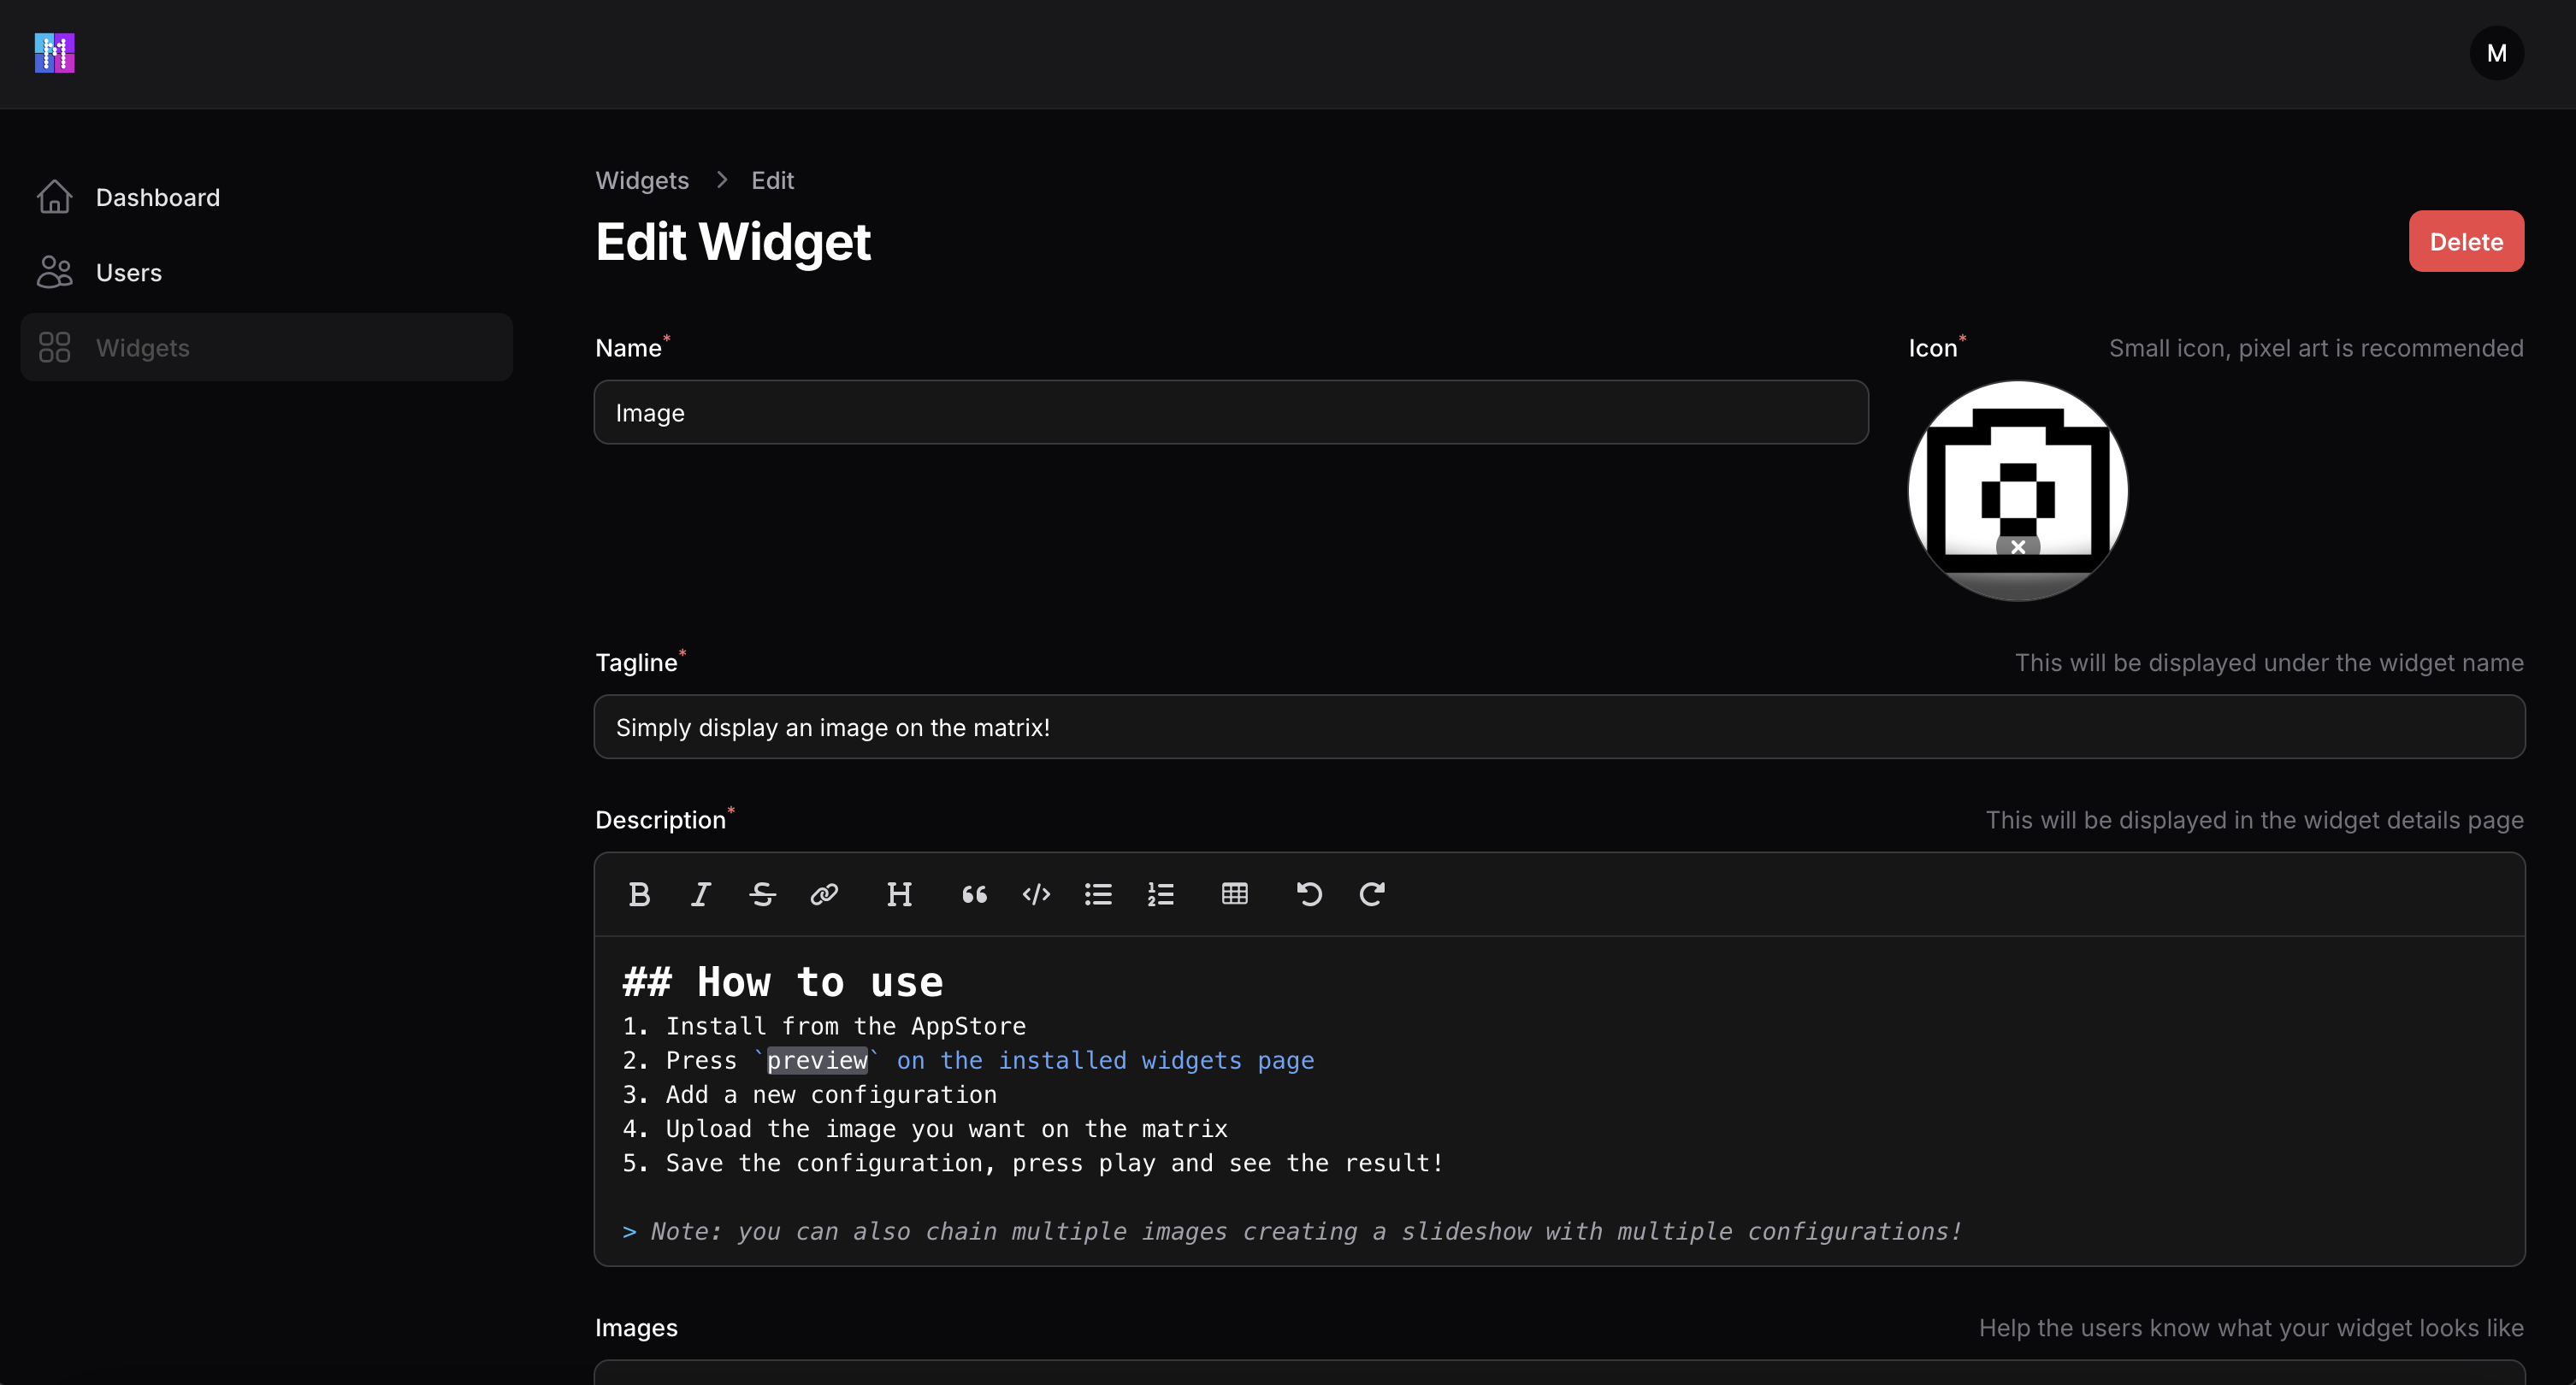
\includegraphics[width=\textwidth]{tesi/img/website_demo/widget-details.png} \caption*{Edit Widget} \end{minipage} \begin{minipage}[b]{0.49\textwidth} \centering 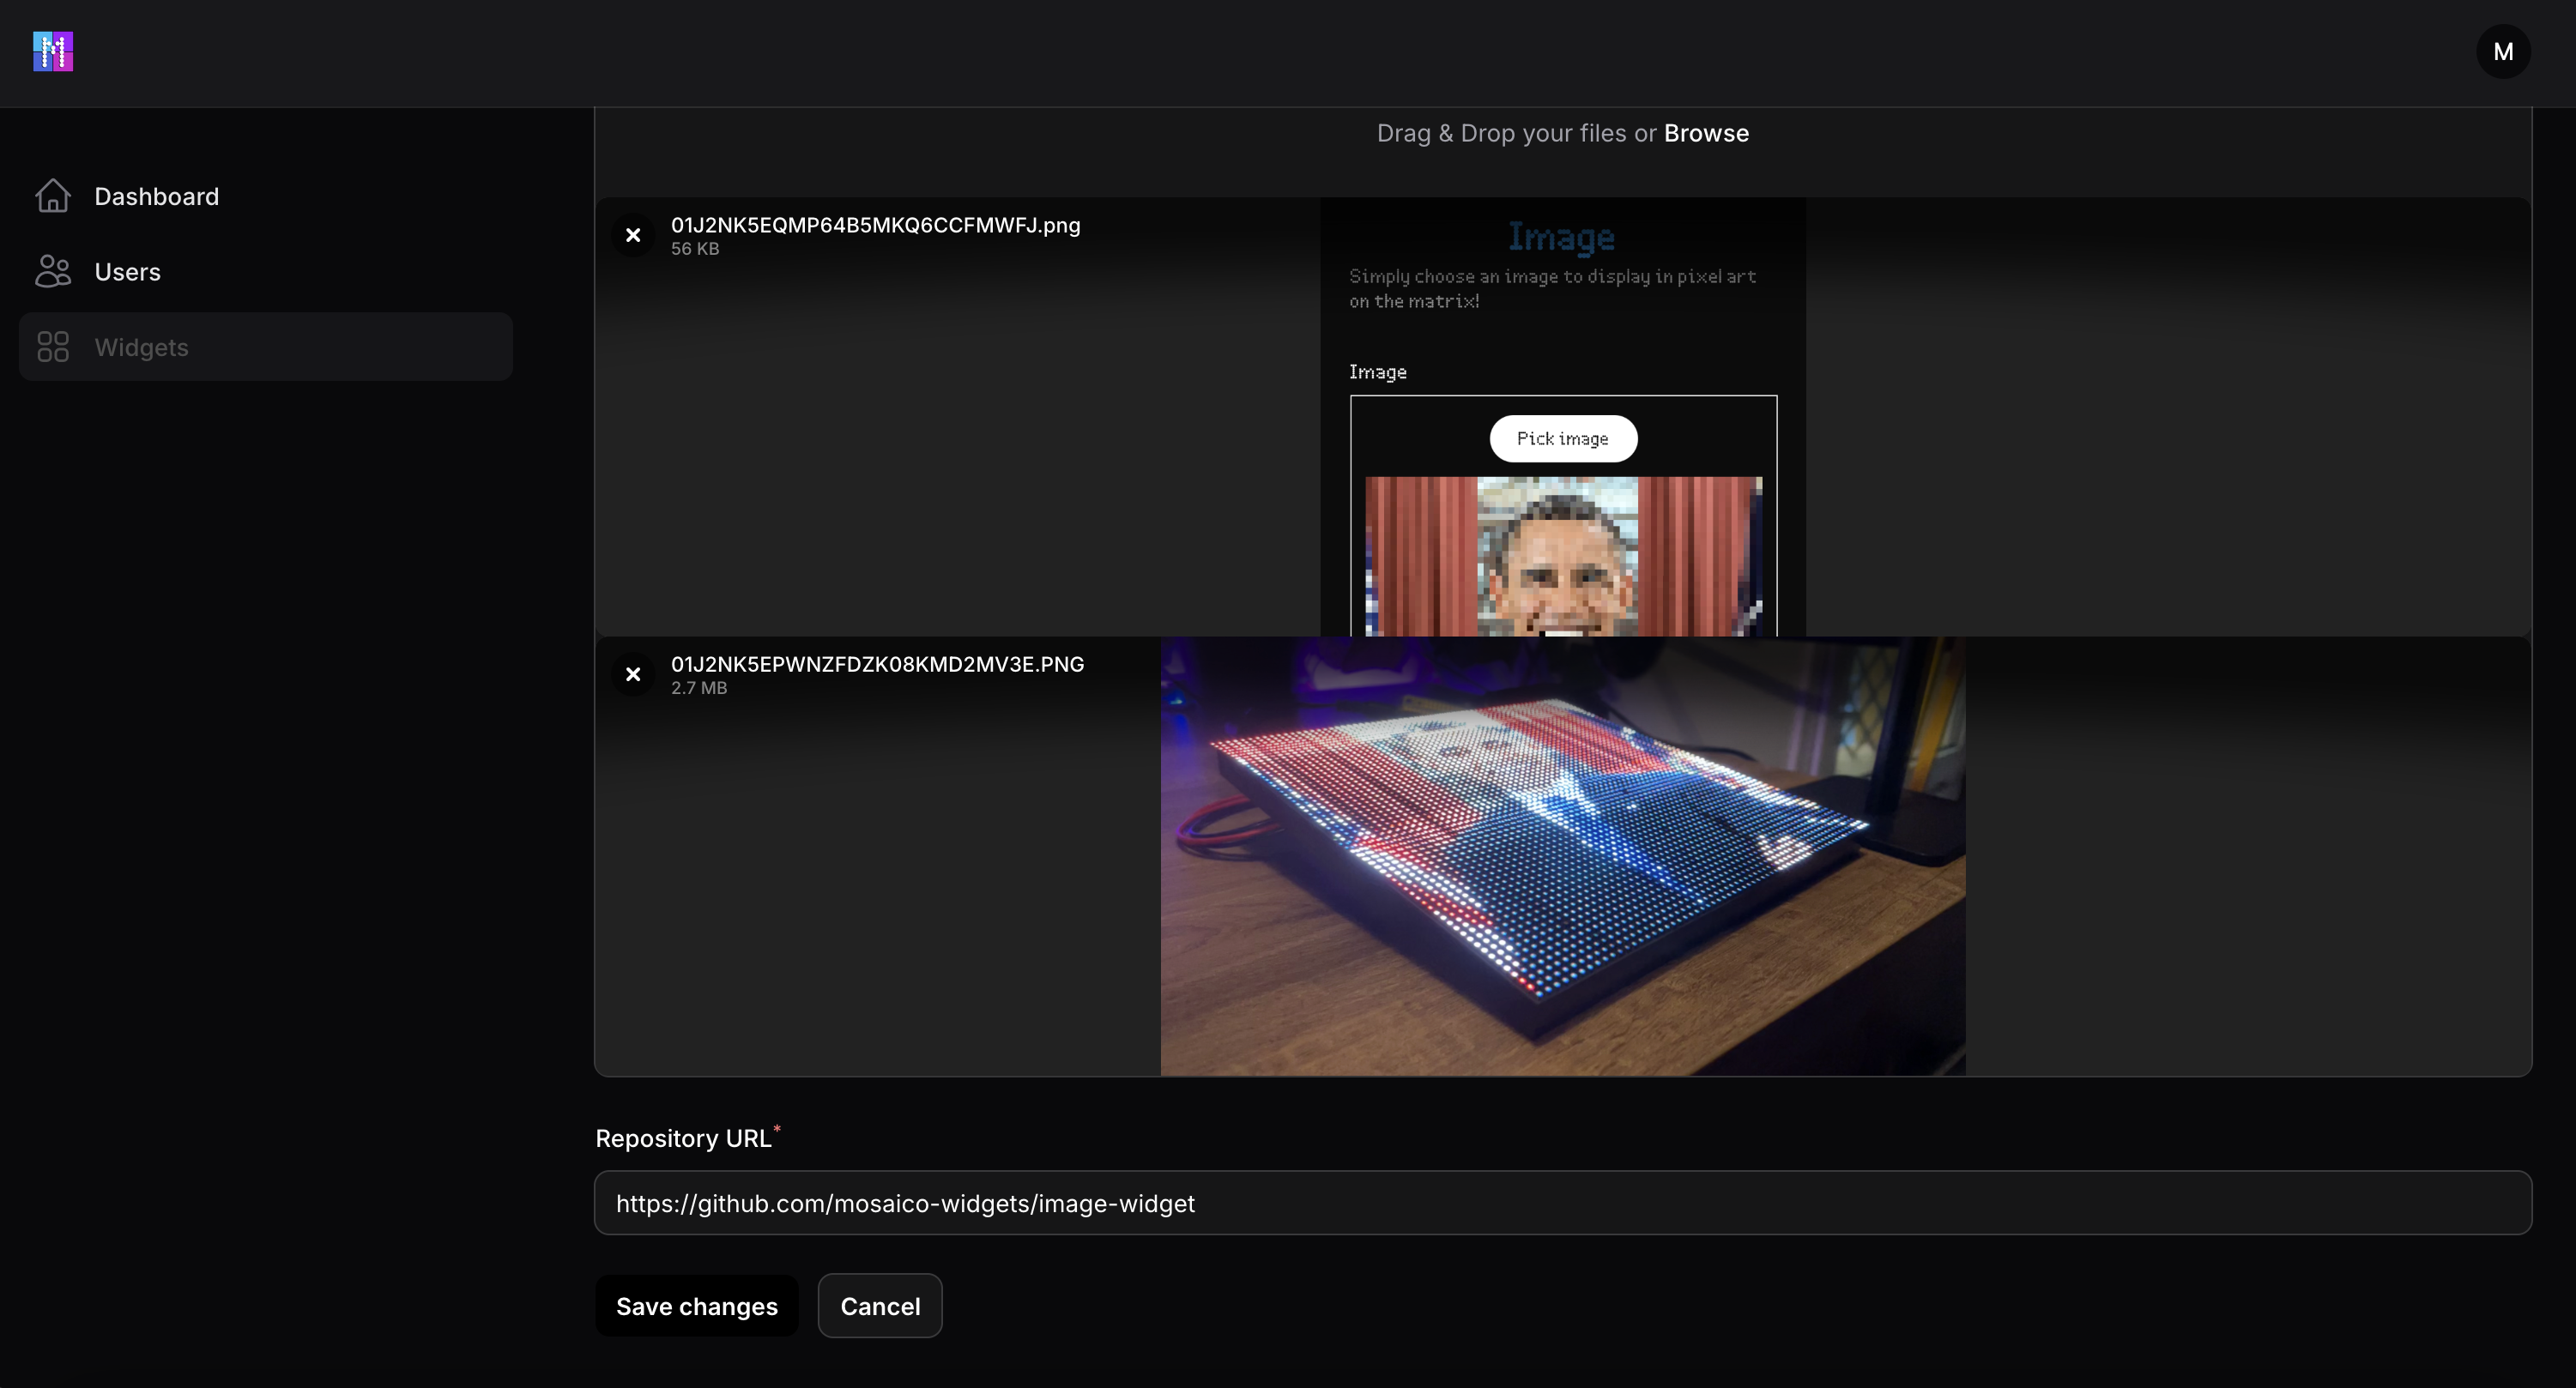
\includegraphics[width=\textwidth]{tesi/img/website_demo/widget-details-2.png} \caption*{Edit Widget - Continued} \end{minipage} \end{figure}

Once all necessary fields have been completed and the developer saves their submission, the widget becomes immediately available to the community.

\section{API}
In the Laravel project, a straightforward REST API is implemented, offering a user-friendly interface for interacting with the Mosaico app store. The API endpoints are designed to be simple and intuitive:

\begin{center} \makebox[\textwidth]{ 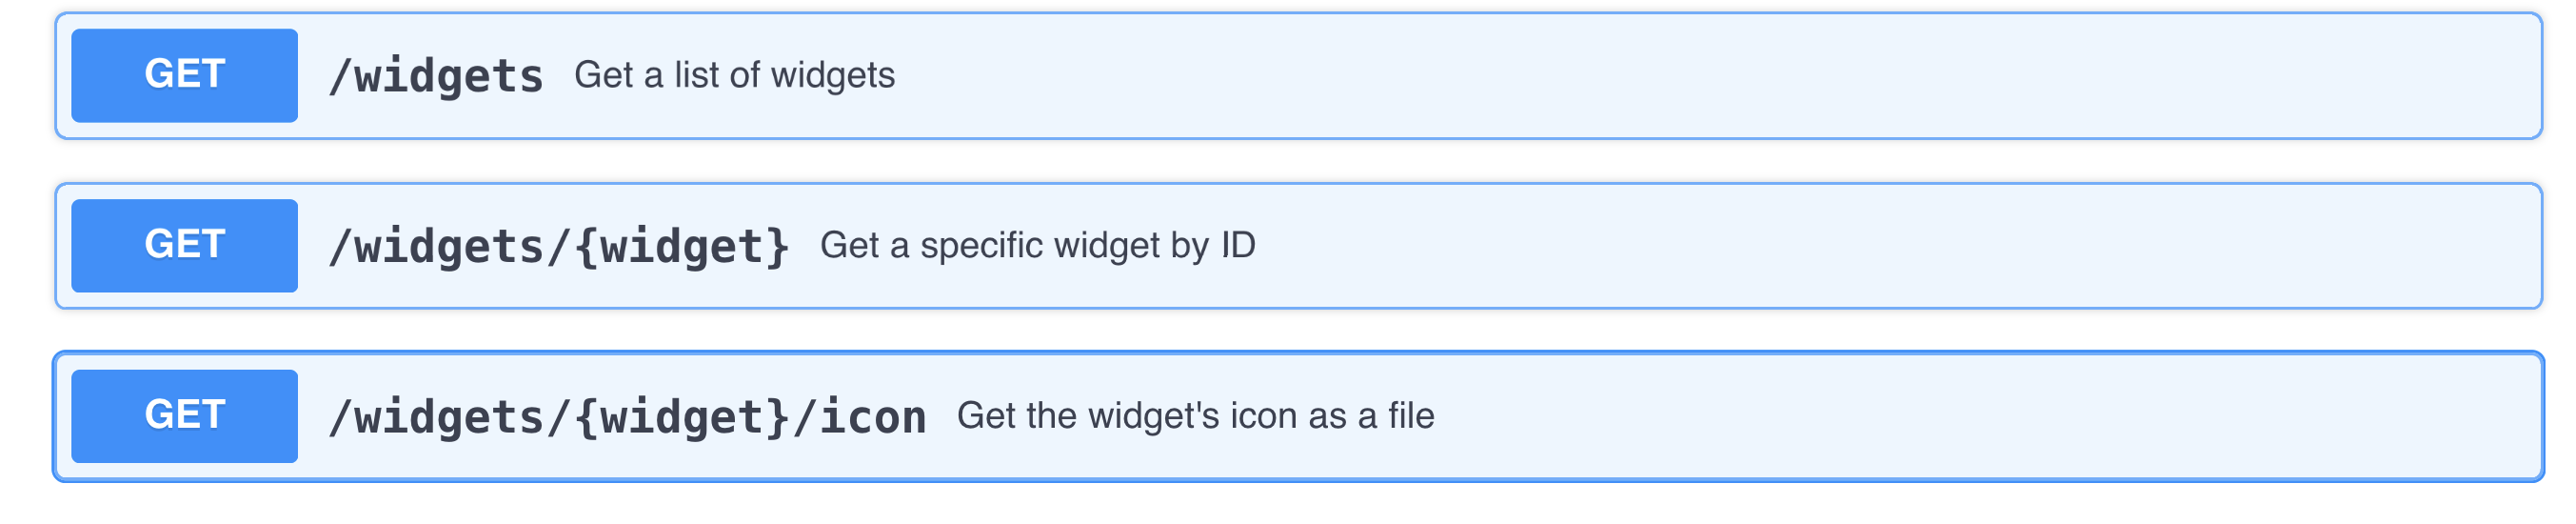
\includegraphics[width=0.8\paperwidth]{tesi/img/website_demo/api.png} } \end{center}

\subsection{Rate Limiter} Given that the only authenticated section of the application is the developer's dashboard, the API remains open for public access, allowing users to browse and utilize its features. However, this accessibility introduces potential vulnerabilities, such as Distributed Denial of Service (DDoS) attacks or spam requests. To mitigate these risks and protect the application’s logic as well as its database from excessive strain, a rate limiting mechanism has been implemented. This mechanism restricts the number of incoming requests from a specific IP address, effectively blocking those that exhibit suspicious behavior.
\newpage
\section{Landing Page}
A well-designed and visually appealing landing page is crucial as the introductory interface for my project. To achieve this, I focused on creating a catchy, minimalistic, and attractive design that effectively captures the essence of Mosaico while ensuring user engagement. The aesthetic appeal of the landing page not only draws users in but also facilitates intuitive navigation, enabling visitors to quickly locate the information and features they seek.

The website can be accessed at \url{https://mosaico.murkrowdev.org}. From this central hub, users can explore all the web-based functionalities of the application. This includes access to the developer dashboard, which allows for seamless interaction with the platform's development tools, as well as links to the project's GitHub repository, where users can contribute to or modify the source code. Additionally, comprehensive documentation is provided, guiding users through the various features and capabilities of Mosaico. This multi-faceted approach ensures that users have all the necessary resources at their fingertips, fostering an environment of collaboration and innovation within the community.

\begin{figure}[H]
\centering
\begin{minipage}[b]{0.49\textwidth}
\centering
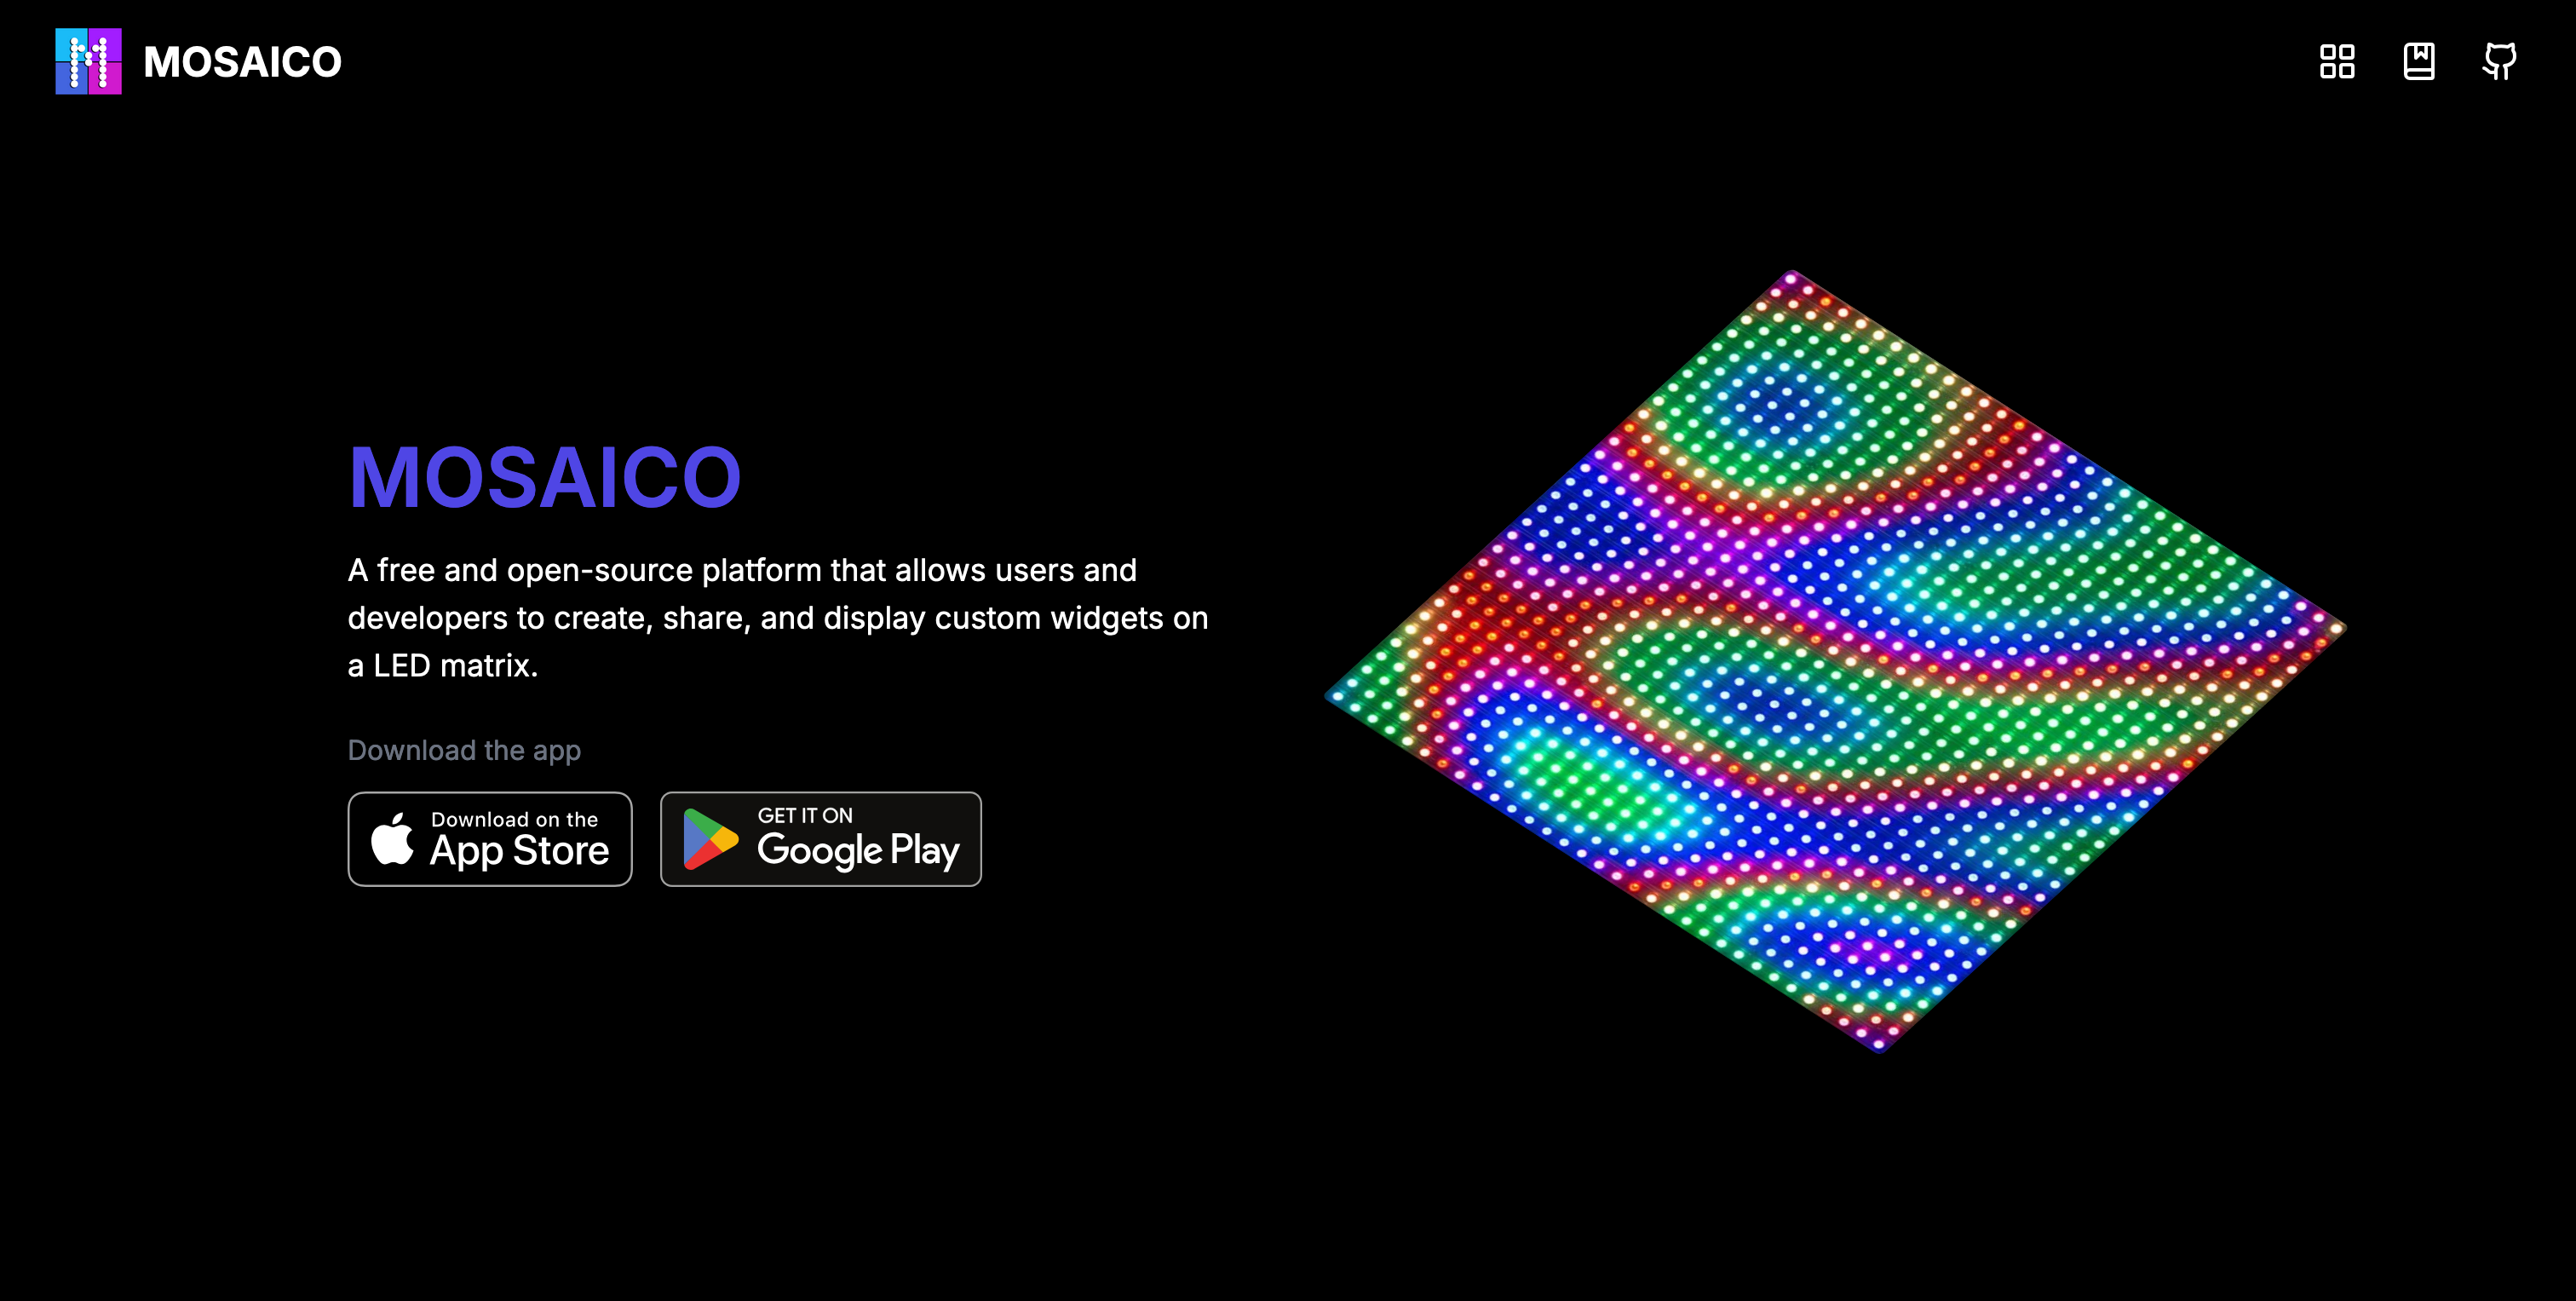
\includegraphics[width=\textwidth]{tesi/img/website_demo/landing/1.png}
\caption*{Call to action}
\end{minipage}
\begin{minipage}[b]{0.49\textwidth}
\centering
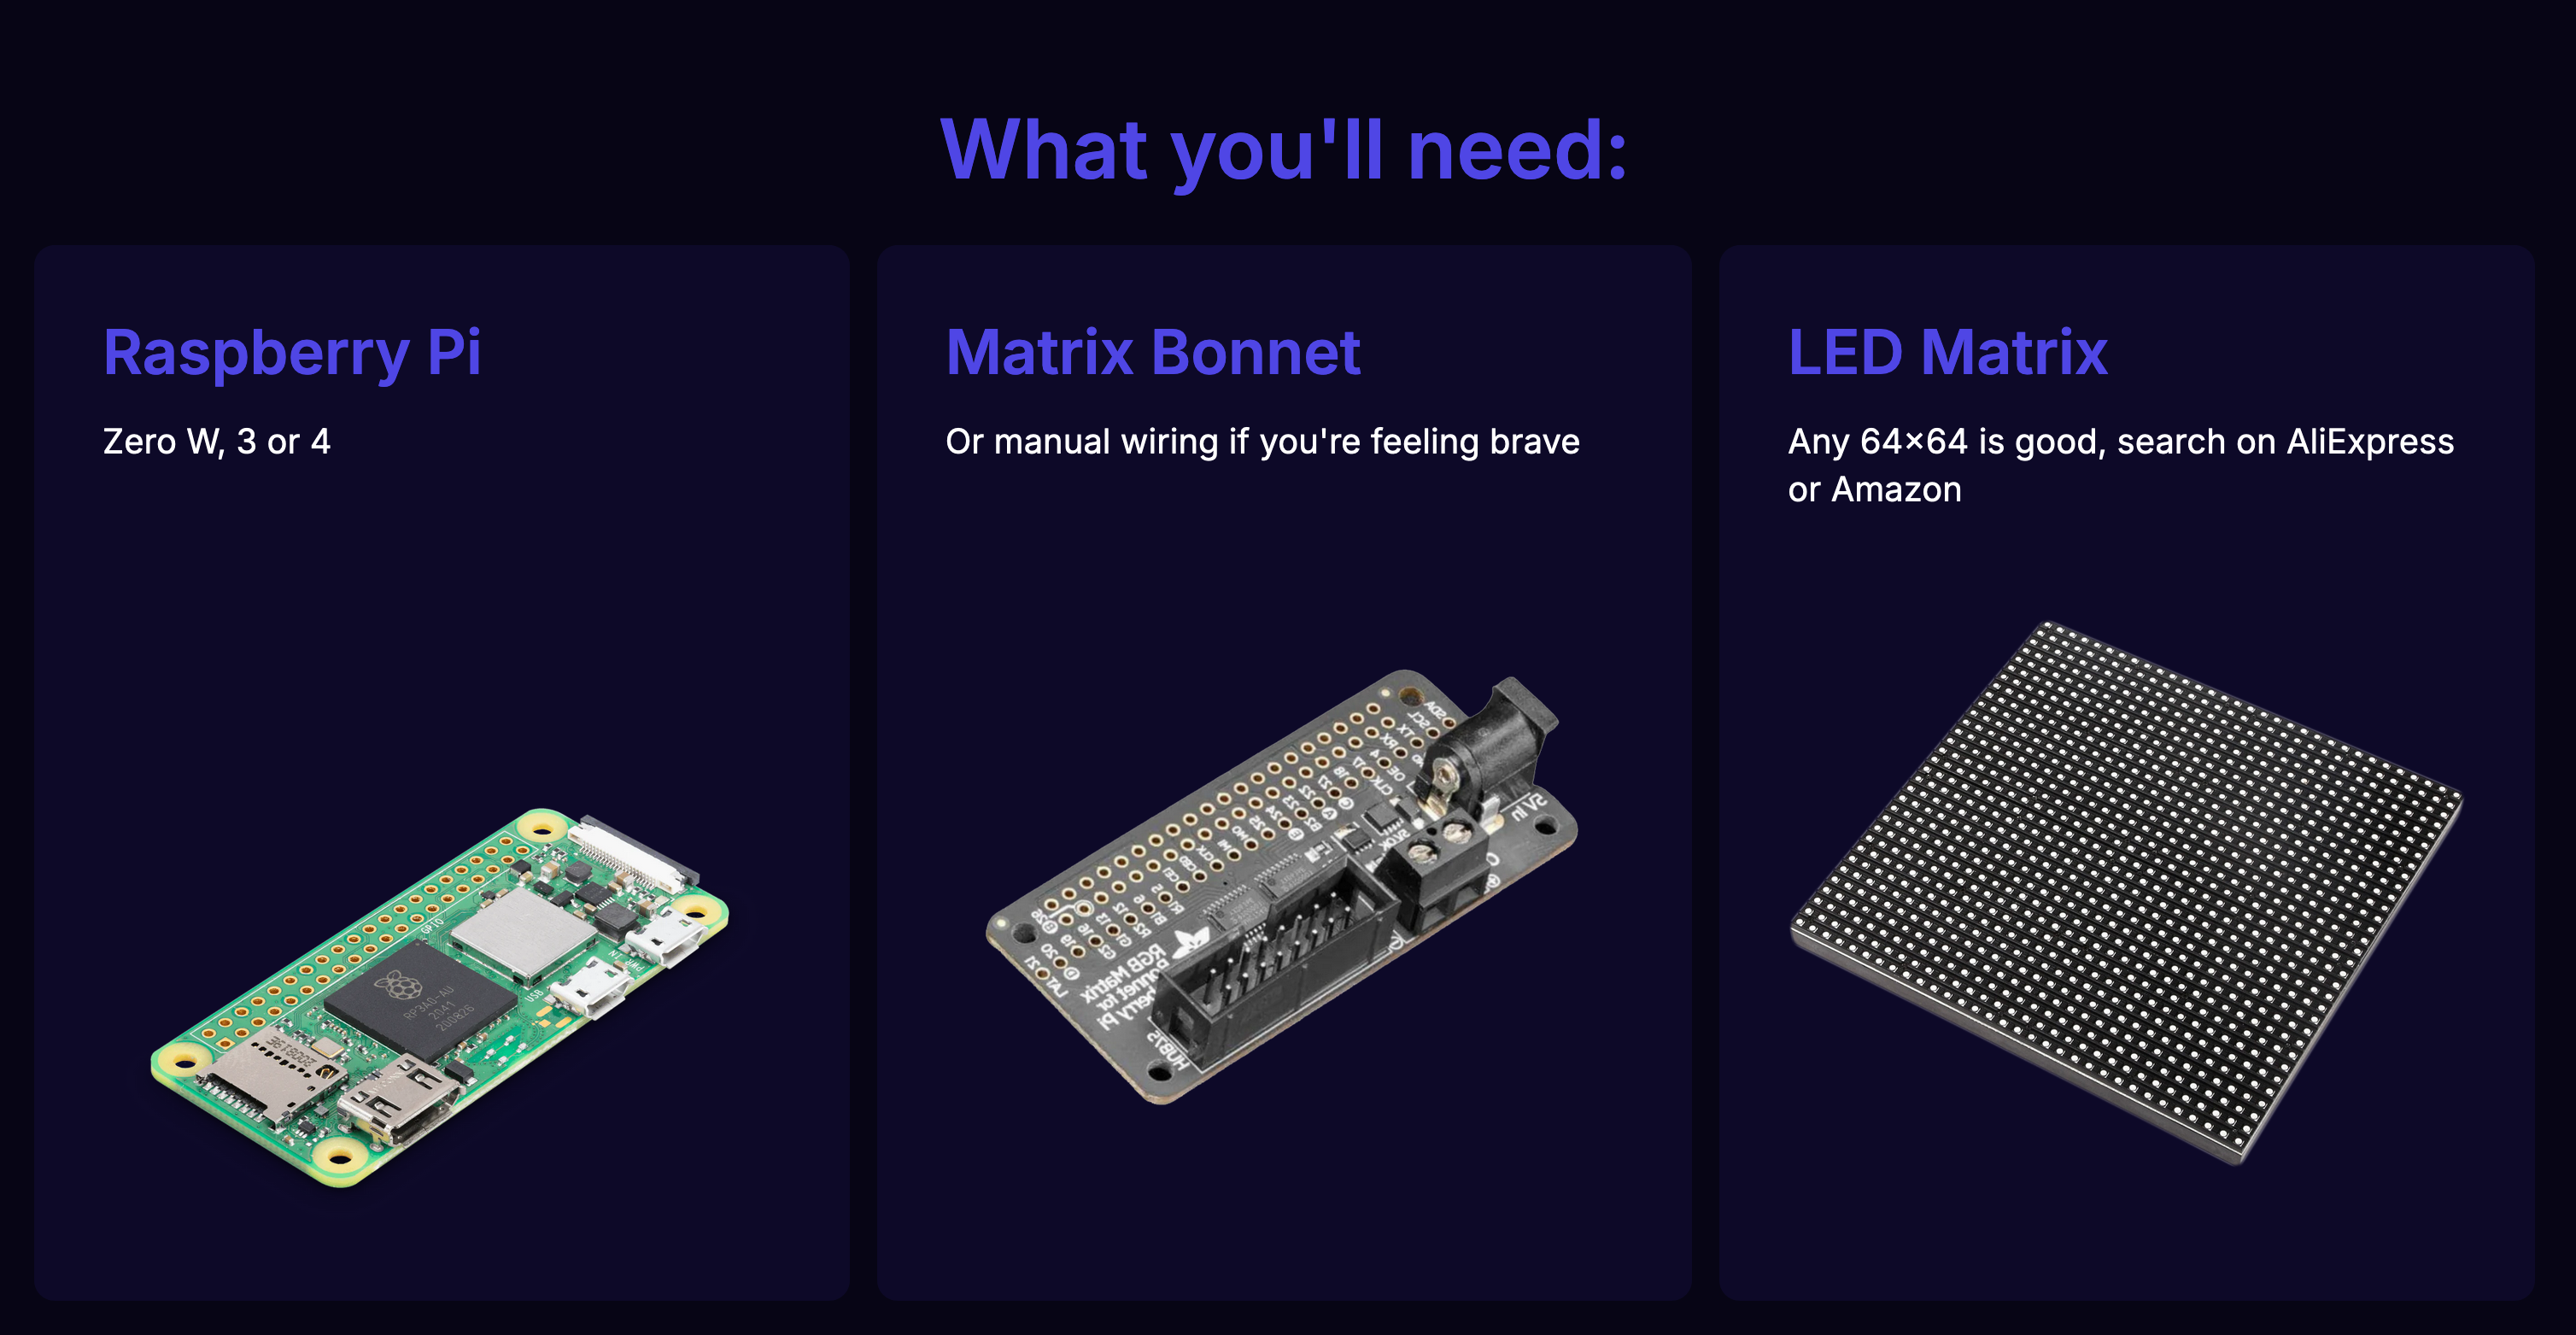
\includegraphics[width=\textwidth]{tesi/img/website_demo/landing/2.png}
\caption*{Hardware components}
\end{minipage}
\end{figure}

\begin{figure}[H]
\centering
\begin{minipage}[b]{0.49\textwidth}
\centering
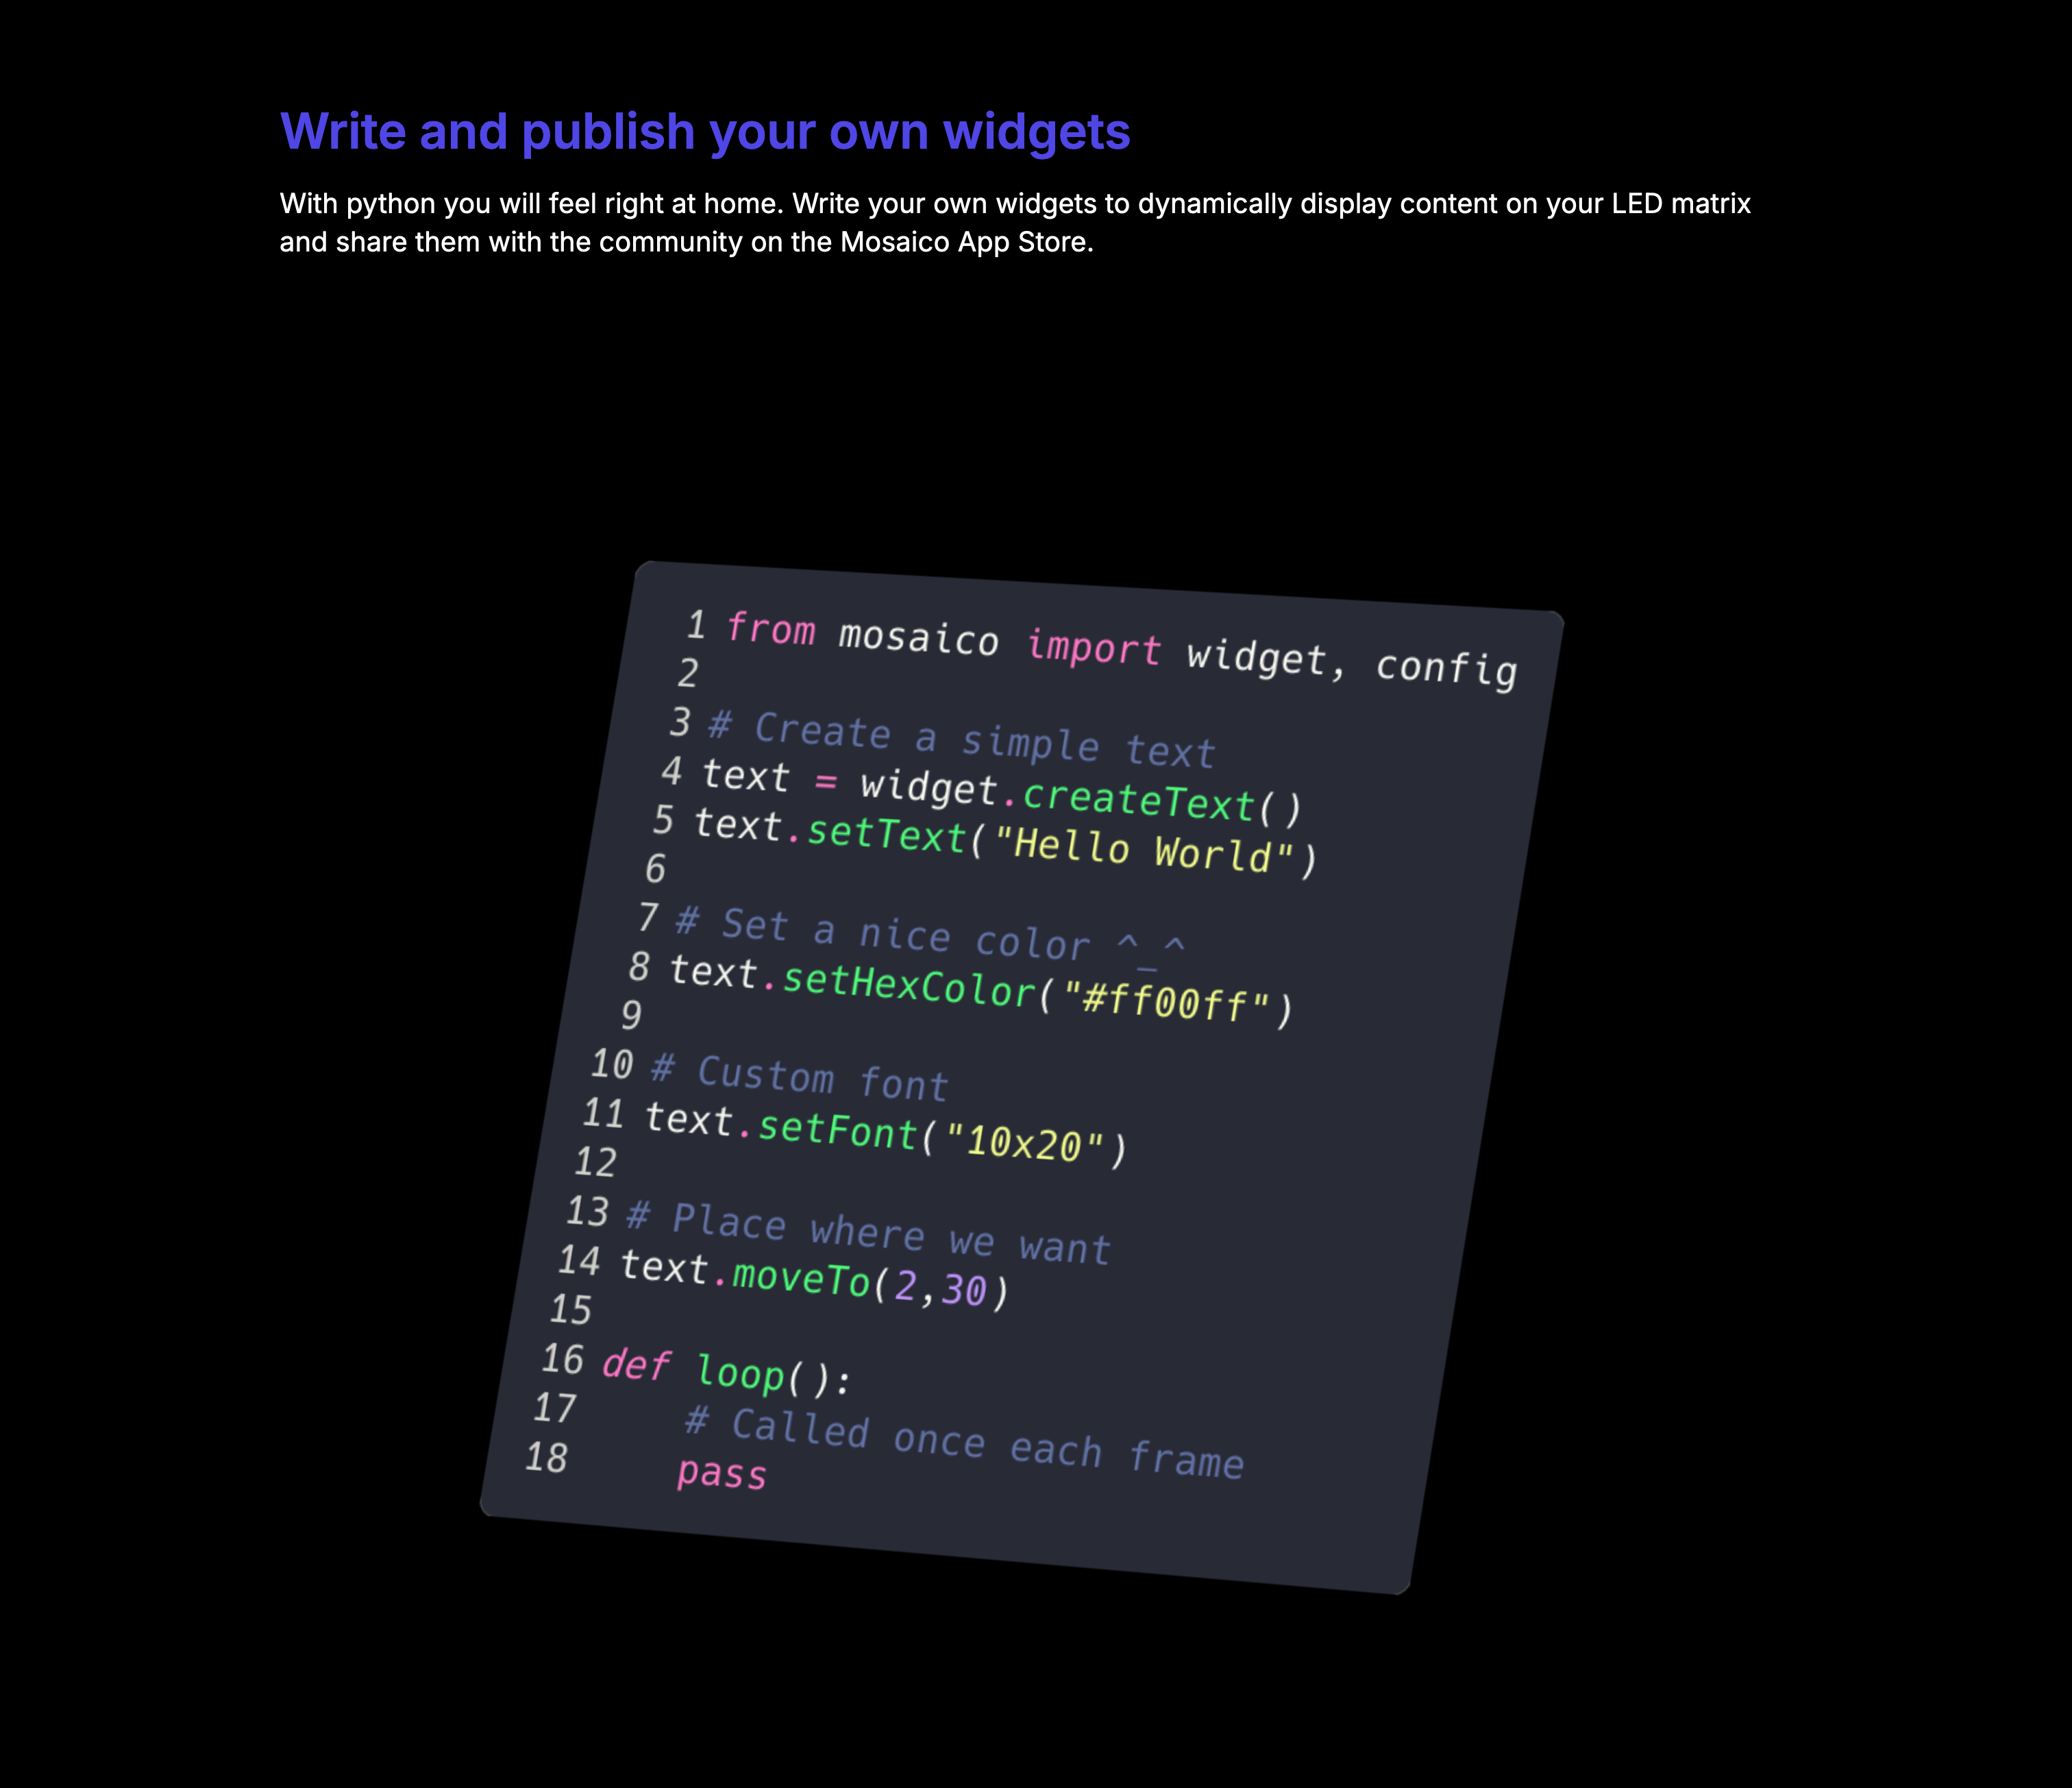
\includegraphics[width=\textwidth]{tesi/img/website_demo/landing/3.png}
\caption*{Widgets}
\end{minipage}
\begin{minipage}[b]{0.49\textwidth}
\centering
\includegraphics[width=\textwidth]{tesi/img/website_demo/landing/4.png}
\caption*{Widgets showcase}
\end{minipage}
\end{figure}

\begin{figure}[H]
\centering
\begin{minipage}[b]{0.49\textwidth}
\centering
\includegraphics[width=\textwidth]{tesi/img/website_demo/landing/5.png}
\caption*{The ecosystem}
\end{minipage}
\begin{minipage}[b]{0.49\textwidth}
\centering
\includegraphics[width=\textwidth]{tesi/img/website_demo/landing/6.png}
\caption*{FAQ}
\end{minipage}
\end{figure}

\newpage
\section{Documentation}
When developing an open-source project, the importance of well-structured and comprehensive documentation cannot be overstated. Effective documentation serves as a vital resource for users and developers alike, providing essential guidance and facilitating engagement with the project. For this purpose, I utilized MkDocs\footnote{\url{https://www.mkdocs.org/}}, a powerful static site generator that enables the creation of documentation using Markdown. This tool allows for the automatic generation of a well-formatted and organized static HTML website, which is readily deployable within my main Laravel project.

The documentation is accessible at the following URL: \url{https://mosaico.murkrowdev.org/docs}. It provides a general overview of the Mosaico project, outlining its objectives and features. However, the primary focus of the documentation is directed towards widget developers aspiring to create and publish widgets in the app store. By offering detailed instructions, examples, and best practices, the documentation aims to empower developers to effectively engage with the Mosaico ecosystem, fostering creativity and collaboration within the community.

\chapter{Testing and deployment}
\section{Benchmarks}
The final version of the \textit{Mosaico} software has been tested for performance on the actual Raspberry Pi hardware, focusing on both CPU and memory usage. These tests yielded satisfactory results, especially considering the hardware limitations of the Raspberry Pi Zero.

\subsection{CPU Usage}

The CPU performance was measured across various scenarios, ranging from idle states (with no widgets displayed) to the execution of the most complex widget available. As shown in the figure below, the CPU usage started at approximately 60\% when no widgets were active, increasing to nearly 80\% when displaying the most demanding widget.

\begin{figure}[H]
    \centering
    \begin{minipage}[b]{0.98\textwidth}
        \centering
        \includegraphics[width=\textwidth]{tesi/img/benchmarks/CPU.png}
        \caption*{CPU performance on a Raspberry Pi Zero (Single Core 1GHz)}
    \end{minipage}
\end{figure}

These results are particularly noteworthy considering the Raspberry Pi Zero operates with a single-core 1GHz processor. Despite these hardware constraints, \textit{Mosaico} demonstrates a considerable degree of efficiency, with room for further optimization. This provides confidence that even more complex widgets can be handled with only marginal increases in CPU load.


\subsection{Memory Usage}
Memory consumption was another key area of focus during performance testing. The use of a lightweight operating system, such as DietPi, proved to be a wise choice, as it minimized the overall system resource usage while maintaining sufficient memory for the app's modules to function efficiently.

\begin{figure}[H]
    \centering
    \begin{minipage}[b]{0.32\textwidth}
        I achieved excellent results even regarding RAM usage, with both my app modules occupiyng only about 15\% of the total system memory while DietPI allowed to run using only about 17\% of total system usage. Remember that the Raspberry Pi Zero has only about 477Mb of usable memory so my software used about 70Mb of memory.
    \end{minipage}
    \begin{minipage}[b]{0.65\textwidth}
        \centering
        \includegraphics[width=\textwidth]{tesi/img/benchmarks/RAM.png}
        \caption*{System RAM utilization}
    \end{minipage}
\end{figure}

\subsection{Conclusion}

The performance benchmarks highlight that \textit{Mosaico} runs efficiently on a minimal system setup like the Raspberry Pi Zero, utilizing only a modest portion of CPU and memory resources. This efficiency allows for a seamless user experience without overburdening the hardware, and it opens the door for future optimizations that can further improve performance. These findings underscore the app's capability to run effectively even on low-powered devices, making it accessible to a wider range of users.
\newpage
\section{Latency}
\subsection{Protocol Performance: CoAP}

In assessing the overall responsiveness and snappiness of the \textit{Mosaico} app, one of the primary metrics evaluated was the performance of the Constrained Application Protocol (CoAP), which is the key communication protocol used to control the matrix features. Given the constrained environment in which the system operates, particularly on a Raspberry Pi Zero, it was crucial to determine how well CoAP could handle request processing and data transfer between system components.

The results of the testing were highly satisfactory. As predicted, CoAP demonstrated excellent performance, with the majority of basic requests—such as activating, stopping, or switching widgets—being processed in approximately 100 milliseconds. This level of efficiency is particularly impressive when considering the hardware limitations. The minimal latency observed during the testing indicates that CoAP is well-suited for real-time interactions between the app and the matrix device, ensuring a smooth user experience even under constrained conditions.

\begin{center}
  \makebox[\textwidth]{
  \includegraphics[width=0.8\paperwidth]{tesi/img/benchmarks/COAP.png}}
\end{center}

One notable exception to the generally fast performance was the installation of new widgets from the app's store, which took approximately 8 seconds. This longer duration can be attributed to two main factors: the need to download files from an external Git repository and the relatively slow storage access speeds of the Raspberry Pi Zero. While this delay is understandable, particularly in a resource-constrained environment, it highlights an area for potential optimization in future iterations of the system.

CoAP proved to be an efficient and reliable protocol for managing communication between the app and the matrix device, delivering swift responses in most use cases while leaving room for improvement in more resource-intensive operations like widget installations.


\section{User Feedback}

User feedback has played a pivotal role in refining \textit{Mosaico}, especially given the project's complexity and its reliance on hardware that might not be readily available to all testers. To address this, I developed web simulators \ref{web-simulator} that allowed users to interact with the app in a virtual environment, greatly expanding the range of people able to provide feedback.

Testers identified several key areas for improvement, including both functional bugs and UI/UX enhancements. For example, some users pointed out issues such as notification stacking, where notifications could overlap in an unintuitive way. This feedback was instrumental in identifying and resolving the problem before the official release.

Moreover, several testers suggested improvements for transitions between widgets, which have now been implemented to create a smoother, more visually appealing experience. Others noted that adding additional widget features, such as previews of fonts or new widgets ideas.

Overall, the feedback provided by early testers has been invaluable in refining the app and ensuring that \textit{Mosaico} is more intuitive, stable, and feature-rich for all users.


\section{Deployment} Perhaps one of the least glamorous but most critical aspects of software development is the deployment process. Transitioning the entire project, along with its various dependencies, to a new machine can be both technically challenging and time-consuming. Ensuring that the development environment mirrors the production environment is essential for a seamless deployment, but achieving this can often be fraught with difficulties.

Fortunately, over the past few years, I have been utilizing Docker, which has drastically streamlined my development and deployment processes. Docker enables the creation of isolated, containerized environments that replicate the production environment with minimal overhead. This ensures consistency between local development and live deployment, significantly reducing the likelihood of environment-specific issues. For this project, I employed a set of custom scripts to dockerize the Laravel application\footnote{\url{https://github.com/codexdevelopment-it/dockerized-laravel}}, alongside all required services such as the database and proxy, to get the entire application up and running smoothly.

\subsection{Self-Hosting} A relatively recent but highly rewarding endeavor I embarked upon is self-hosting. About a year ago, I ventured into this fascinating domain, purchasing a dedicated server to host all my internal and public services, thereby eliminating the need to rely on external VPS providers. Self-hosting not only grants full control over the infrastructure but also reduces long-term operational costs, as I am no longer paying recurring fees to third-party hosting providers.

The server's infrastructure is virtualized using Proxmox\footnote{\url{https://www.proxmox.com/}}, a robust, open-source platform for enterprise-level virtualization. Proxmox's comprehensive feature set includes a web-based interface that simplifies the management of virtual machines (VMs), containers, software-defined storage, and networking. This has greatly enhanced my ability to manage complex projects and services efficiently.

When deploying a new project, I simply create a new Linux Container (LXC) with Docker support, clone the repository, and execute a predefined bash script to initiate the deployment process. The entire system is up and running in minutes. Additionally, I configure a new subdomain for the project and use a reverse proxy with automatic HTTPS support\footnote{\url{https://caddyserver.com/}} to direct traffic to the corresponding container. One of the key advantages of this setup is the ease with which I can manage backups—thanks to Proxmox's virtualized storage volumes, I can create incremental backups of entire disks rather than backing up individual files, significantly simplifying the backup and restore process.

This self-hosting infrastructure has provided me with a highly flexible, cost-effective, and scalable environment in which I can develop, deploy, and manage my projects with ease.

\subsection{AppStore and PlayStore}
Publishing the application on both the Apple App Store and Google Play Store was a pivotal moment in making my project accessible to a broad audience. Since I used Flutter as the core development framework, the cross-platform compatibility significantly simplified the process of handling Android fragmentation. With Flutter, I was able to write a single codebase that worked seamlessly across both platforms, ensuring that the user experience was consistent and smooth on various devices.

The app only requires Bluetooth and photo access, both of which are essential for configuring the LED matrix widgets. Bluetooth is used for connecting to the matrix device, while photo access allows users to upload images for specific widgets. Beyond these two permissions, the project has a strict policy against data collection or remote storage. Staying true to the open-source philosophy, the app does not collect or store user data in any remote database, offering users more control and privacy. This adherence to privacy meant that the often tedious privacy approval process became much smoother, as there was no sensitive data being transferred or stored, allowing for a quicker review.

Being fully open-source further reinforces the transparency of the application. Users can inspect the code, ensuring that no hidden data collection mechanisms exist, which adds trust and aligns with the core values of user empowerment and privacy.

\chapter{Conclusion}
The core achievements of this project can be distilled into the successful development of the mobile app, Raspberry Pi software, and web platform, each aligned with the outlined goals. The mobile app offers an intuitive, responsive user experience with seamless matrix control and caching mechanisms that reduce strain on the Raspberry Pi. The Raspberry Pi software itself remains efficient, modular, and well-documented, allowing developers to easily create or modify widgets. The web platform is both visually appealing and easily deployable, serving as the backbone for the widget store and developer interactions.

One of the project’s most important long-term objectives lies in its open-source nature. By embracing open-source principles, the project encourages collaboration, transparency, and customization, offering more value to users. No data is collected, preserving user privacy, and the entire platform is designed to benefit from community engagement. The next phase of this project will focus on pushing it further into open-source channels, gaining momentum through developer contributions, user feedback, and widespread adoption. Through community involvement, the platform can continue to grow, integrate new features, and enhance functionality, paving the way for a sustainable, innovative future.



\renewcommand{\bibsection}{}
\chapter*{Bibliographical references}
\bibliography{tesi/refs}
\newpage

\newpage~\newpage
\chapter*{Acknowledgements}
This project would not have been possible without the incredible contributions from the open-source community. A special thanks goes to Henner Zeller for his brilliant C++ library to control the LED matrix\footnote{\url{https://github.com/hzeller/rpi-rgb-led-matrix}} and to Adafruit for their LED matrix bonnet and setup guide\footnote{\url{https://learn.adafruit.com/}}. The Nlohmann JSON library\footnote{\url{https://github.com/nlohmann/json}}, pybind11\footnote{\url{https://github.com/pybind/pybind11}}, aiocoap\footnote{\url{https://github.com/chrysn/aiocoap}}, and bless\footnote{\url{https://github.com/kevincar/bless}} libraries provided seamless integration between Python and C++, ensuring robust communication between modules. Tools such as GitPython\footnote{\url{https://github.com/gitpython-developers/GitPython}} and Docker\footnote{\url{https://www.docker.com/}} significantly streamlined the development and deployment processes.

A huge thank you also goes to JetBrains for their educational licenses of IDEs like PHPStorm\footnote{\url{https://www.jetbrains.com/phpstorm/}}, CLion\footnote{\url{https://www.jetbrains.com/clion/}}, and PyCharm\footnote{\url{https://www.jetbrains.com/pycharm/}}, which greatly facilitated the development across different project components.

Lastly, while ChatGPT\footnote{\url{https://chat.openai.com/}} proved invaluable in mastering Flutter and Python and speeding up development processes, it was used as a learning aid rather than a coding substitute, reinforcing concepts and helping resolve challenges faster without replacing the core development effort.

\end{document}




\chapter{Introduction}
\input{tesi/chapters/1.0}

\chapter{State of the Art}
\input{tesi/chapters/0}




\pagestyle{plain}




\section{Objectives}
\input{tesi/chapters/1.2}

\section{Hardware components}
\input{tesi/chapters/1.3}

\section{Widgets}
\input{tesi/chapters/1.4}


\chapter{Project Architecture}
\input{tesi/chapters/2.0}

\section{Software}
\input{tesi/chapters/2.1}

\newpage
\section{Client}

\input{tesi/chapters/2.2}

\section{Web}
\input{tesi/chapters/2.3}

\section{Simulator}
\input{tesi/chapters/2.4}

\chapter{Networking}
\input{tesi/chapters/3.0}

\chapter{Programming with AI}

\chapter{Feedback}


\renewcommand{\appendixtocname}{Appendici}
\renewcommand{\appendixpagename}{Appendici}
% \csname @openrightfalse\endcsname
\pagenumbering{gobble}
\begin{appendices}
\chapter{Appendice 1}
\label{Appendice:A}
Probabilmente ci sono un sacco di package non utilizzati ma così funziona tutto quindi non ho indagato oltre.

Inoltre su internet c'è un sacco di documentazione se ti servisse.
\chapter{Appendice B}
\label{Appendice:B}
Appendice B se serve

\chapter{Embed di interi PDF}
\label{Appendice:C}
Se ti serve puoi fare embed di PDF interi con pdfpage, scegliendo anche le pagine (o mettendo - se le vuoi tutte):

\includepdf[pages=1]{pdf/sample.pdf}
\end{appendices}
\end{comment}

